% ===================== Lattice data & extracting the x-dependence (thesis Ch. 5) =====================
\section{Lattice data}

\begin{frame}{The $x$-dependent Sivers shift}
  Write $\nu=b\cdot P$ and keep $s=-b_\mu b^\mu$, $\zetahat$, and $\eta v\cdot P$ fixed:
  \[
    \tAmp_{iB}^{[x]}(s,x,\zetahat,\eta v\cdot P)
    =\int_{-\infty}^{\infty}\frac{d\nu}{2\pi}\,
      e^{ix\nu}\tAmp_{iB}(s,\nu,\zetahat,\eta v\cdot P).
  \]
  \[
    \langle k_y\rangle_{TU}(s,x,\zetahat,\eta v\cdot P)
    =m_N\frac{\tilde f_{1T}^{\perp(1)}(s,x,\zetahat,\eta v\cdot P)}
                  {\tilde f_1^{(0)}(s,x,\zetahat,\eta v\cdot P)}
    =-m_N\frac{\tAmp_{12B}^{[x]}}{\tAmp_{2B}^{[x]}}.
  \]
  \begin{itemize}
    \item In the lattice frame, $s=b_L^2+b_T^2$. In the TMD frame with $b^+=0$, $s=|\vect b_{T,\mathrm{TMD}}|^2$.
    \item The Fourier transform varies $\nu$ at fixed $s$; it is not a transform at fixed lattice $b_T$.
    \item The common soft factor cancels at fixed geometry under the multiplicative-renormalization assumption used in the thesis.
  \end{itemize}
  \figsrc{Thesis, Ch. 5: Sivers shift as a function of momentum fraction $x$.}
\end{frame}

\begin{frame}{Cosine and sine transforms of the complex amplitudes}
  At fixed $(s,\zetahat,\eta v\cdot P)$, define the real quantities
  \begin{align*}
    E_i(x)&=\int_{-\infty}^{\infty}\frac{d\nu}{2\pi}\cos(x\nu)\tAmp_{iB}^{\mathrm{Re}}(\nu),\\
    O_i(x)&=\int_{-\infty}^{\infty}\frac{d\nu}{2\pi}\sin(x\nu)\tAmp_{iB}^{\mathrm{Im}}(\nu).
  \end{align*}
  \[
    \tAmp_{iB}^{[x]}=E_i-O_i+
    i\int_{-\infty}^{\infty}\frac{d\nu}{2\pi}
       [\sin(x\nu)\tAmp_{iB}^{\mathrm{Re}}(\nu)
        +\cos(x\nu)\tAmp_{iB}^{\mathrm{Im}}(\nu)].
  \]
  \begin{itemize}
    \item $\tAmp^{\mathrm{Re}}$ is even and $\tAmp^{\mathrm{Im}}$ odd in $\nu$. The remaining imaginary integral vanishes by parity, when the integrals exist.
    \item Therefore $\tAmp_{iB}^{[x]}=E_i-O_i$ is real. The thesis labels these two real transforms $\tAmp_{iB}^{[x]\mathrm{Re}}$ and $\tAmp_{iB}^{[x]\mathrm{Im}}$.
  \end{itemize}
  \[ \langle k_y\rangle_{TU}=-m_N\frac{E_{12}-O_{12}}{E_2-O_2}. \]
  \figsrc{Thesis, Ch. 5: Fourier decomposition; all transform signs follow $e^{+ix\nu}$.}
\end{frame}

% Slide 21
\begin{frame}{The Collins--Soper parameter $\zetahat$}
  \quick
  \begin{columns}[c]
    \begin{column}{0.55\textwidth}
      \[ \zetahat = \frac{v \cdot P}{\sqrt{|v^2|}\, \sqrt{P^2}} \]
      \begin{itemize}
        \item On the lattice the staple direction $v$ must be space-like ($v^2<0$), purely spatial ($v_0=0$).
        \item The physical TMD limit needs $\zetahat\to\infty$ (light-like $v$).
        \item Larger $\zetahat$ requires larger nucleon momentum $\vect P$.
        \item We track the Sivers shift over several $\zetahat$ and \textbf{extrapolate}.
      \end{itemize}
    \end{column}
    \begin{column}{0.43\textwidth}
      \centering
      \begin{tikzpicture}[scale=0.95]
        \fill[gray!12] (0,0) -- (2,2) -- (-2,2) -- cycle;
        \draw[gray, dashed] (-2,-2) -- (2,2) node[above right, font=\scriptsize] {light cone};
        \draw[gray, dashed] (2,-2) -- (-2,2);
        \draw[-latex] (-2.2,0) -- (2.3,0) node[right] {$z$};
        \draw[-latex] (0,-1.6) -- (0,2.3) node[above] {$t$};
        \draw[-latex, very thick, blue] (0,0) -- (0.9,1.9) node[above, font=\small] {$P$};
        \draw[-latex, very thick, badred] (0,0) -- (-1.9,0.3) node[left, font=\small] {$v$};
        \draw[-latex, thick, badred!50, dashed] (0,0) -- (-1.6,1.35);
        \node[badred, font=\scriptsize, align=right, anchor=north east, fill=white, inner sep=1pt] at (-0.9,-0.95) {$\zetahat\to\infty$: $v$ tilts\\toward the light cone};
      \end{tikzpicture}
      \\[1mm]
      {\scriptsize Generic frame ($\zetahat$ is Lorentz invariant)}
    \end{column}
  \end{columns}
\end{frame}

% Slide 22
\begin{frame}{Kinematic constraint to scan the full $\bvec\tcdot P$}
  \begin{itemize}
    \item The Fourier transform needs both zero and non-zero $\bvec \tcdot P$, but $\dfrac{v \tcdot \bvec}{v \tcdot P} = \bvec \tcdot P\, \dfrac{R(\zetahat^2)}{\mN^2}$ ties the geometry together. With $P = (E, P_1, 0, 0)$:
  \end{itemize}
  \[ b_{1}|v|\left[\frac{P_{1}}{\mN}\left(\zetahat-\sqrt{\zetahat^2+1}\right)+\zetahat\,\frac{\mN}{P_{1}}\right]=\vec{v}_{T}\cdot\vec{b}_{T} \]
  \begin{itemize}
    \item Choose $\vec{v}_{T}=(0,v_{3})$, $\vec{b}_{T}=(b_{2},0)$ $\Rightarrow$ right-hand side $=0$ for every $b_1$, so the bracket must vanish.
  \end{itemize}
  \begin{columns}[t]
    \begin{column}{0.5\textwidth}
      \begin{block}{Example: $P_1=-1$}
        \small
        $\mN = 0.6228(28)/a = 1077.8(48)$ MeV\\
        $P_1=-2\pi/L=-339.8$ MeV
      \end{block}
    \end{column}
    \begin{column}{0.48\textwidth}
      \small
      \[ \zetahat =\sqrt{\frac{P_{1}^2}{\mN^{2}\left(\frac{\mN^{2}}{P_{1}^{2}}+2\right)}} = 0.090772 \]
      \[ \zetahat=\frac{-v_{1}P_{1}}{|v|\,\mN} \ \Rightarrow\ v_{1}=\pm 0.301\,v_{3} \]
    \end{column}
  \end{columns}
\end{frame}

% Slide 23
\begin{frame}{Staple directions $v$ for all four momenta}
  \begin{columns}[c]
    \begin{column}{0.45\textwidth}
      \centering
      \renewcommand{\arraystretch}{1.2}
      \begin{tabular}{ccc}
        \toprule
        $\vect{P}\cdot a\hat{L}/(2\pi)$ & $\zetahat$ & $v_1$ \\
        \midrule
        $(-1,0,0)$ & $0.090772$ & $0.301\,v_3$ \\
        $(-2,0,0)$ & $0.294367$ & $0.531\,v_3$ \\
        $(-3,0,0)$ & $0.539684$ & $0.689\,v_3$ \\
        $(-4,0,0)$ & $0.785756$ & $0.786\,v_3$ \\
        \bottomrule
      \end{tabular}\\[3mm]
      \raggedright
      \begin{itemize}
        \item Lattice parameters: $\vect{\bvec}/a=(b_{1},b_{2},0)$; \ $\eta \vect{v}/a=\eta\,(v_{1},0,v_{3})$, $\eta\in\{0,1,2,3,4,5,6,7,8,9,10\}$; \ $\vect{P}\cdot a\hat{L}/(2\pi)=(n,0,0)$, $n\in\{-1,-2,-3,-4\}$.
        \item $P_L\equiv n$: nucleon momentum in units of $2\pi/(\hat L a)$, $\hat L=32$.
        \item $v$ is \textbf{off-axis} in the $v_1$--$v_3$ plane: not a lattice direction.
      \end{itemize}
    \end{column}
    \begin{column}{0.53\textwidth}
      \centering
      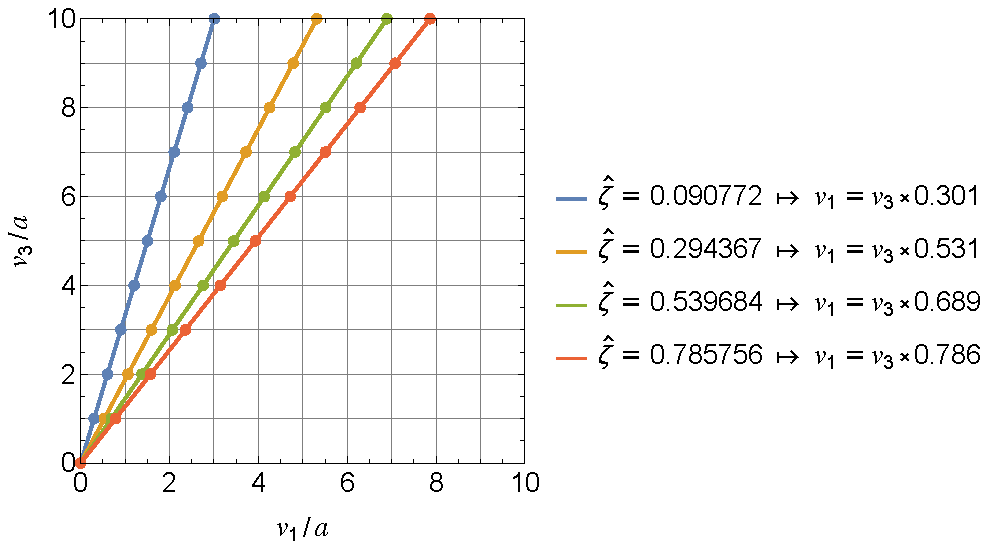
\includegraphics[width=\linewidth]{v1_v2_allzetahat_plot.pdf}
    \end{column}
  \end{columns}
\end{frame}

% Slide 24
\begin{frame}{Bounding lattice paths for each momentum}
  \quick
  \centering
  \begin{tabular}{cc}
    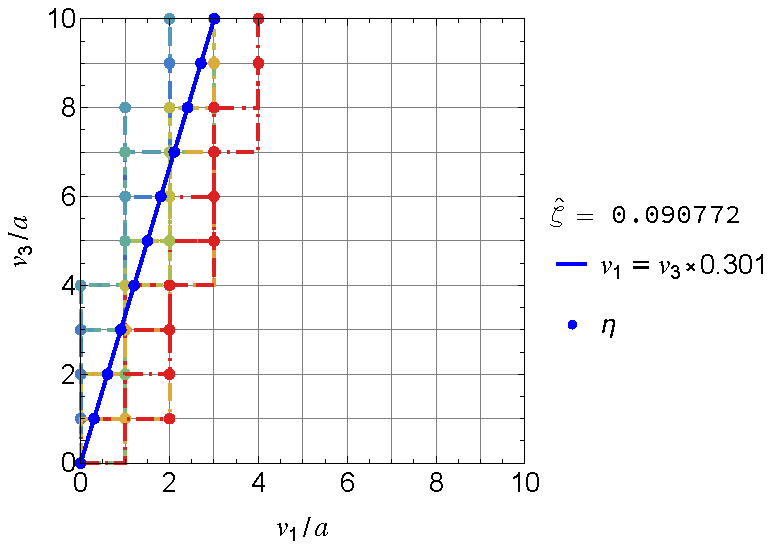
\includegraphics[height=0.37\textheight]{v1_v2_withPath_forP-1_plot.pdf} &
    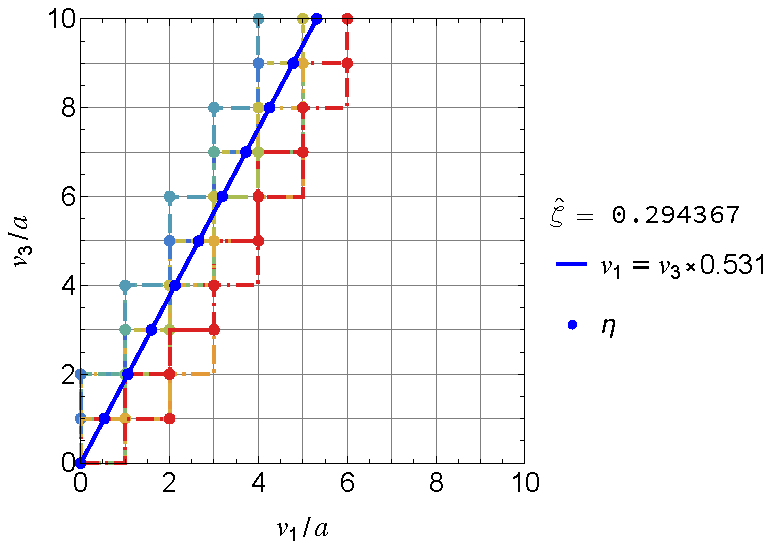
\includegraphics[height=0.37\textheight]{v1_v2_withPath_forP-2_plot.pdf} \\[-1mm]
    {\scriptsize $P_L=-1$, $\zetahat=0.090772$} & {\scriptsize $P_L=-2$, $\zetahat=0.294367$} \\
    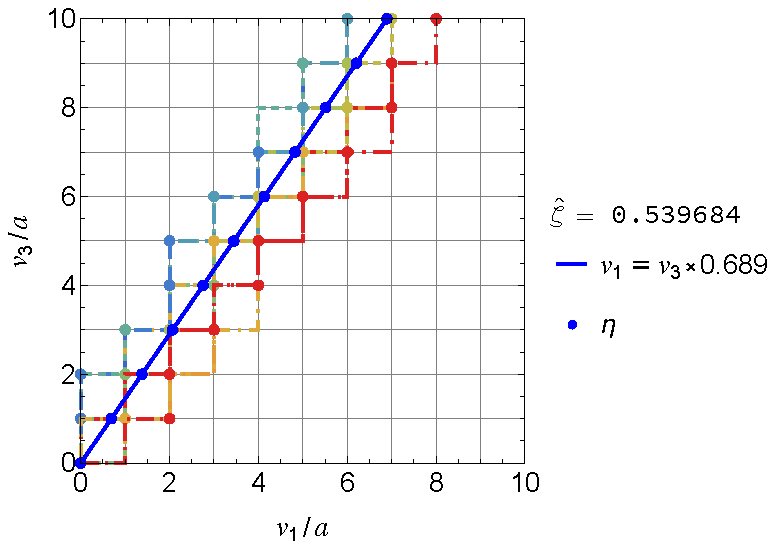
\includegraphics[height=0.37\textheight]{v1_v2_withPath_forP-3_plot.pdf} &
    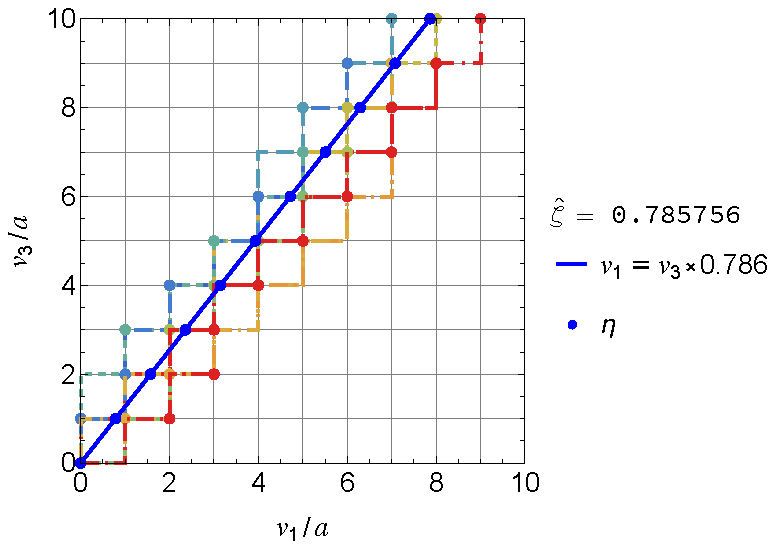
\includegraphics[height=0.37\textheight]{v1_v2_withPath_forP-4_plot.pdf} \\[-1mm]
    {\scriptsize $P_L=-3$, $\zetahat=0.539684$} & {\scriptsize $P_L=-4$, $\zetahat=0.785756$}
  \end{tabular}
\end{frame}

% Slide 25
\begin{frame}{Staple link paths at $P_L=-1$}
  \quick
  \begin{columns}[c]
    \begin{column}{0.36\textwidth}
      \centering
      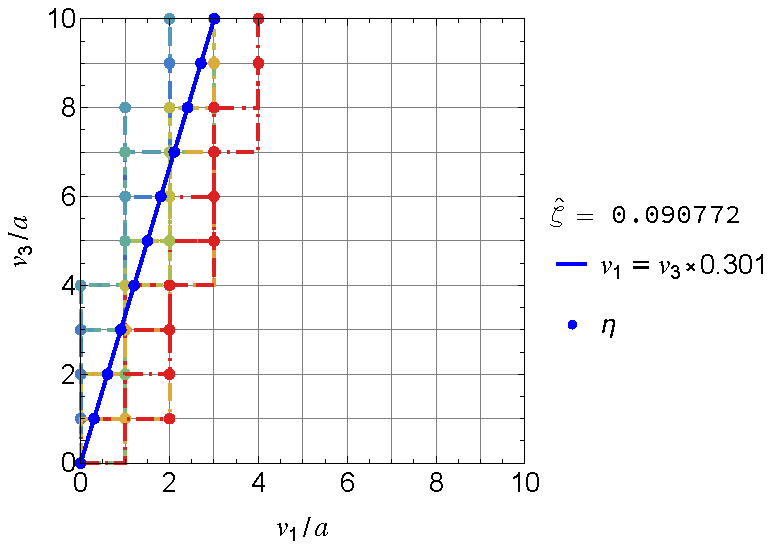
\includegraphics[width=\linewidth]{v1_v2_withPath_forP-1_plot.pdf}\\
      {\scriptsize Integer lattice sites bounding $\eta\vect v/a$}
      \begin{itemize}
        \item For each $\eta$ we compute the correlator at several bounding sites around the target.
      \end{itemize}
    \end{column}
    \begin{column}{0.62\textwidth}
      \centering
      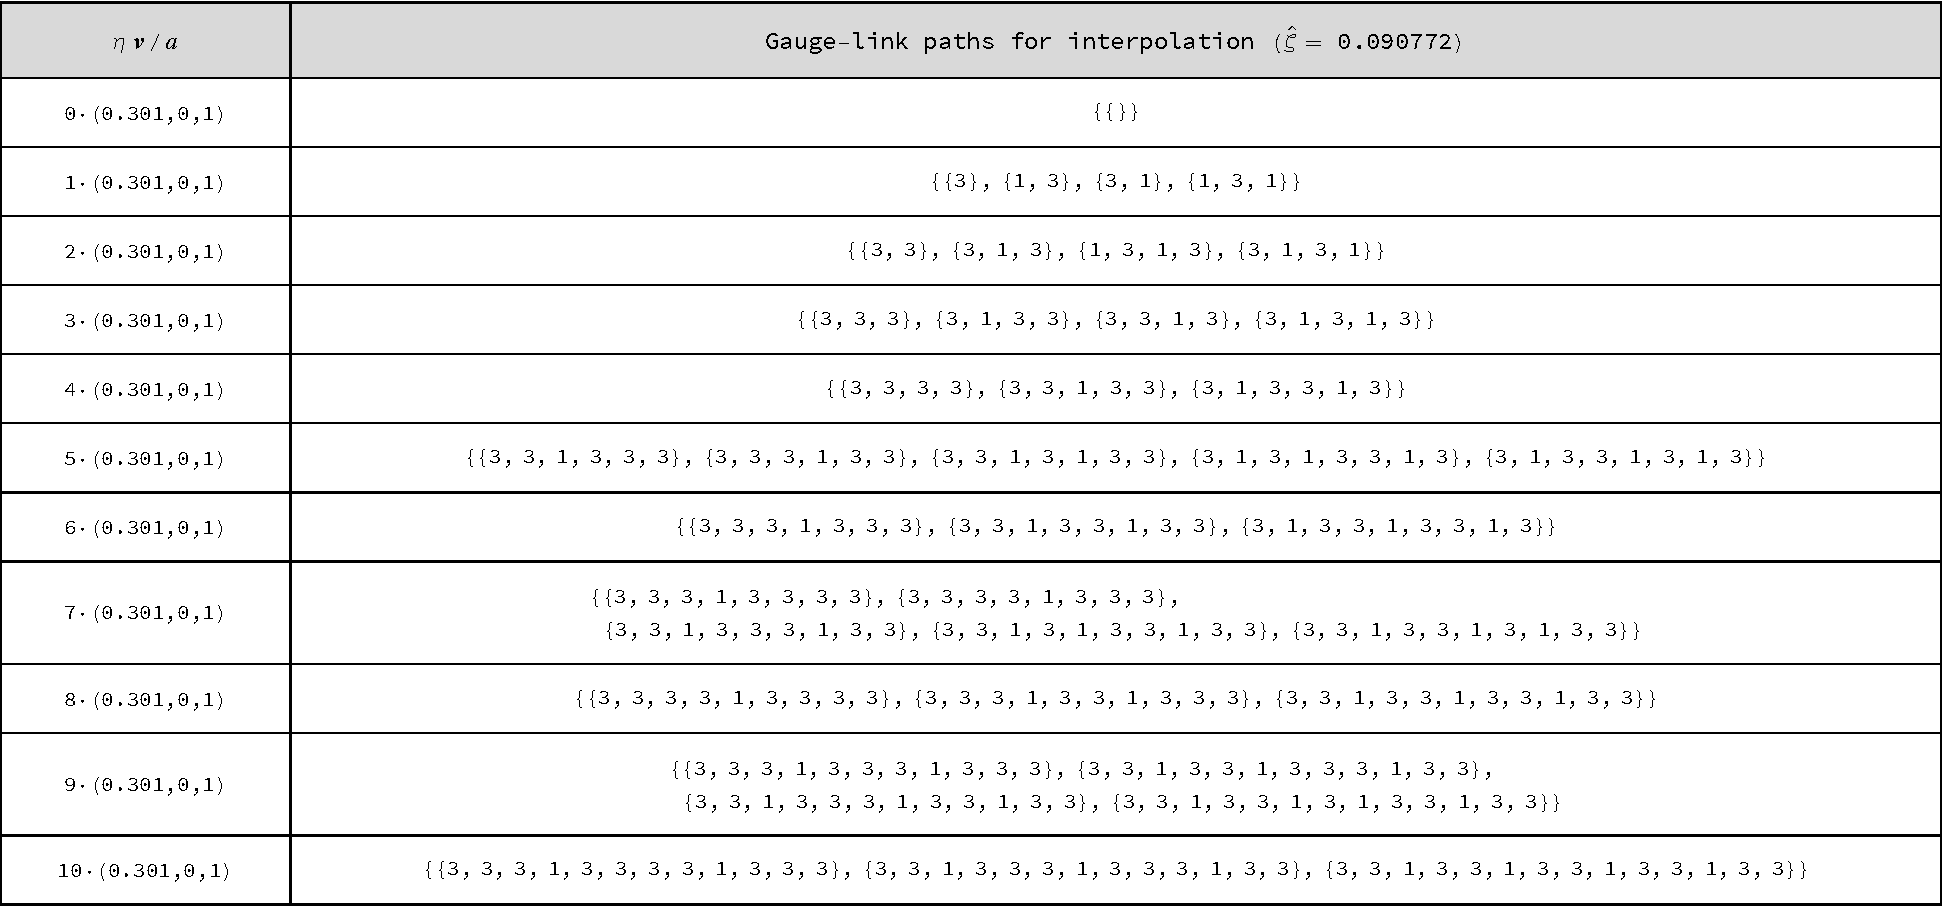
\includegraphics[width=\linewidth]{eta_gauge_links_forP-1_table.pdf}\\
      {\scriptsize Gauge-link step sequences used for interpolation ($\zetahat=0.090772$)}
    \end{column}
  \end{columns}
\end{frame}

\begin{frame}{Staple interpolation paths at $P_L=-2$}
\centering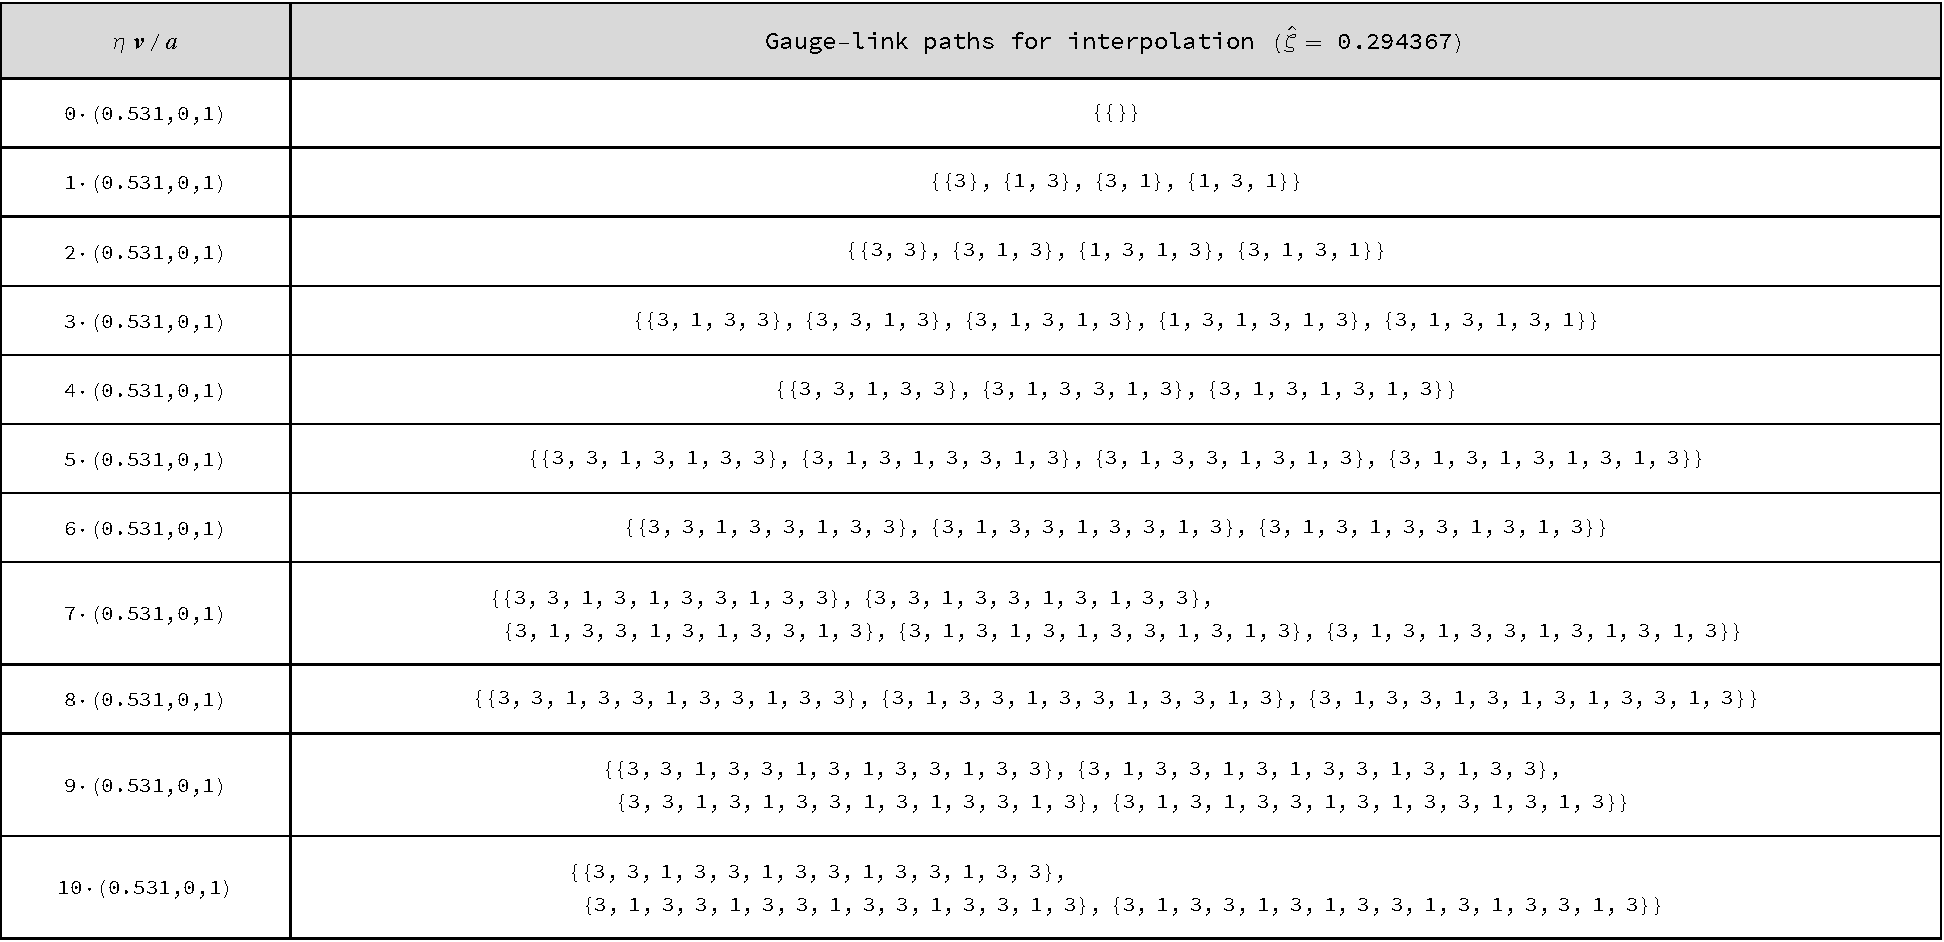
\includegraphics[width=0.97\linewidth,height=0.76\textheight,keepaspectratio]{eta_gauge_links_forP-2_table.pdf}
\figsrc{Thesis, Ch. 5: bounding lattice paths. Arrays list the complete directional step sequence.}
\end{frame}

\begin{frame}{Staple interpolation paths at $P_L=-3$}
\centering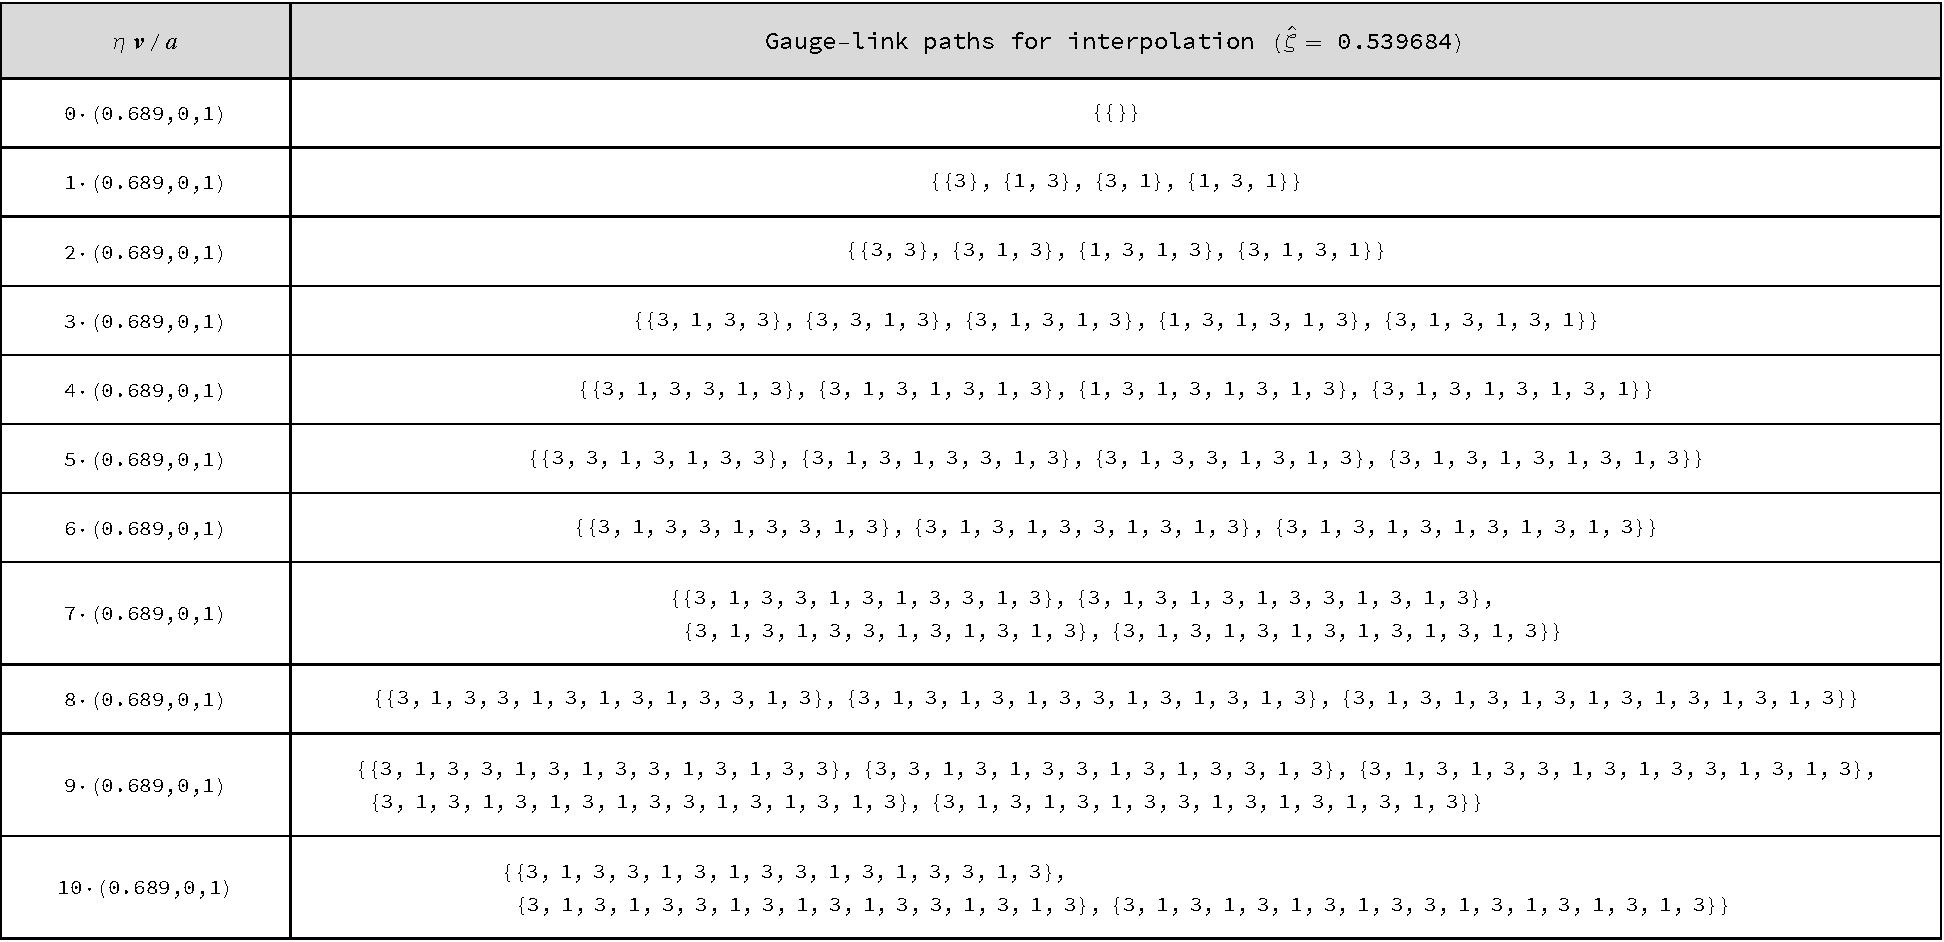
\includegraphics[width=0.97\linewidth,height=0.76\textheight,keepaspectratio]{eta_gauge_links_forP-3_table.pdf}
\figsrc{Thesis, Ch. 5: bounding lattice paths. Arrays list the complete directional step sequence.}
\end{frame}

\begin{frame}{Staple interpolation paths at $P_L=-4$}
\centering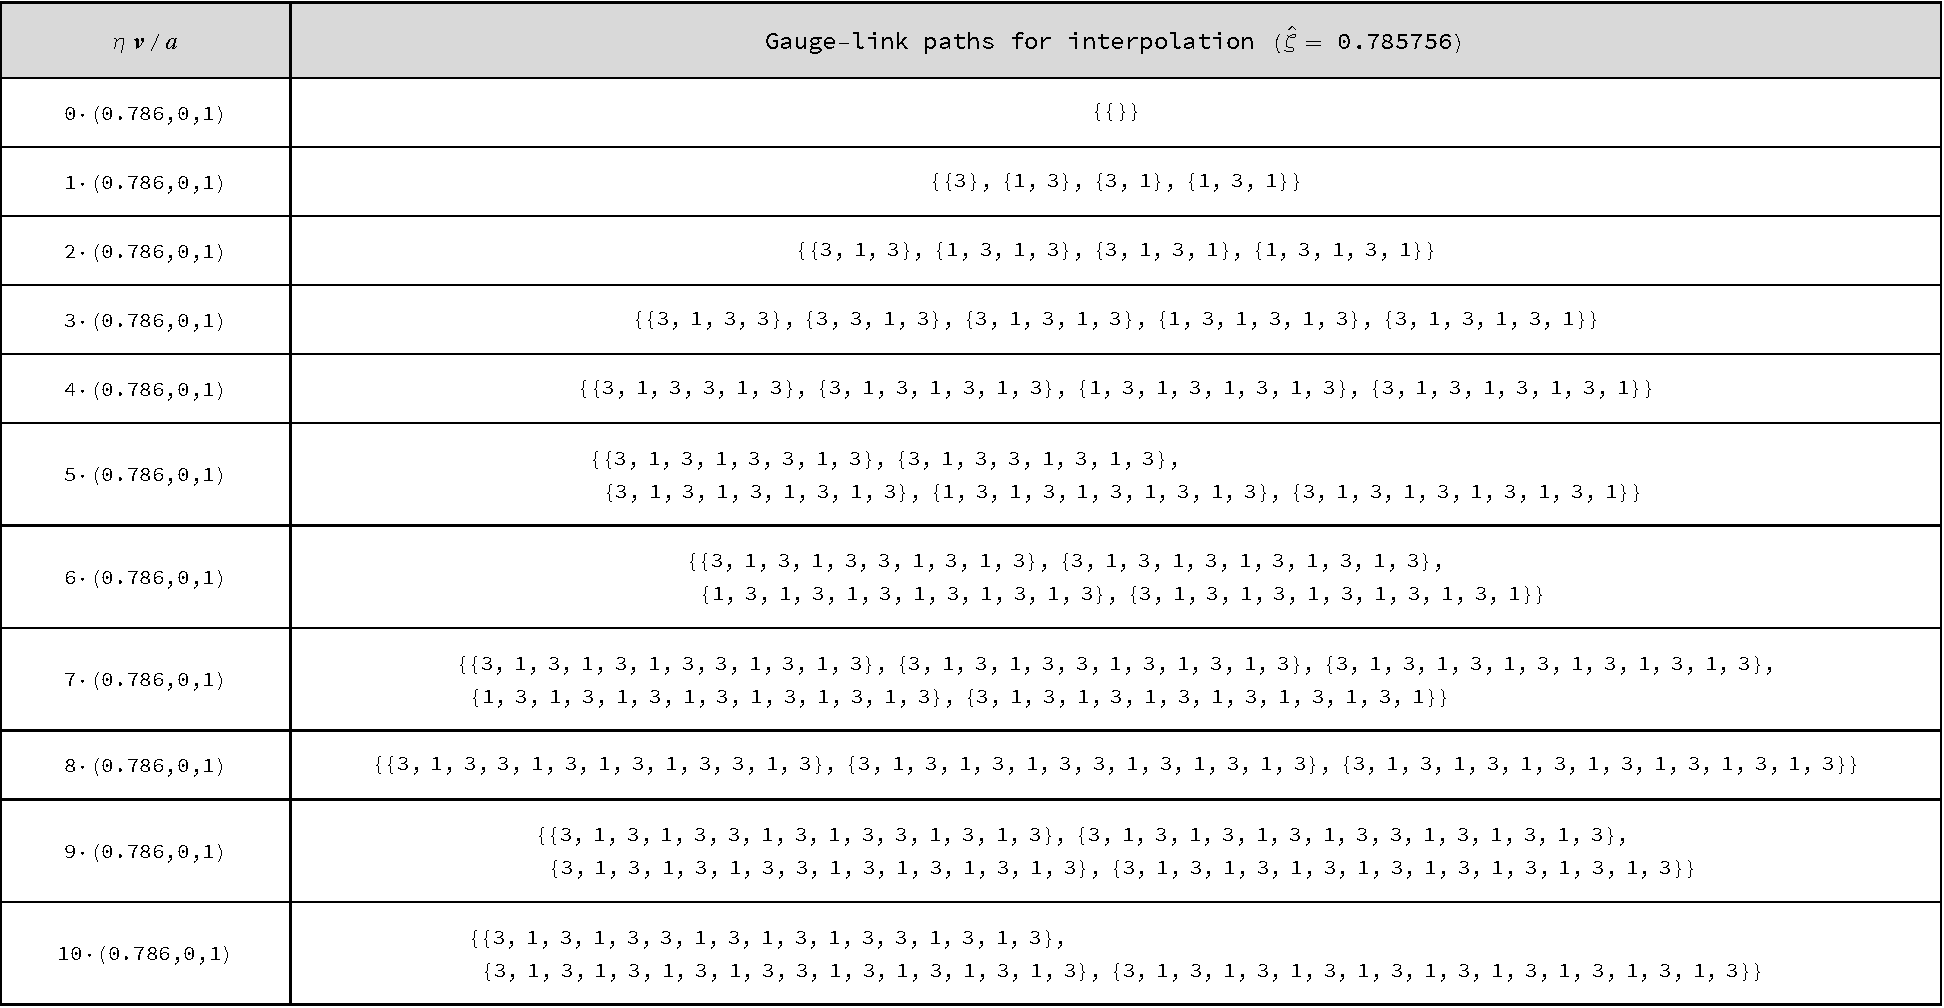
\includegraphics[width=0.97\linewidth,height=0.76\textheight,keepaspectratio]{eta_gauge_links_forP-4_table.pdf}
\figsrc{Thesis, Ch. 5: bounding lattice paths. Arrays list the complete directional step sequence.}
\end{frame}
\begin{frame}{Staple path sequences: $P_L=-1$, $\eta=0$--$2$}
\centering\small
\begin{tabular}{r l}
$\eta=0$ & $\eta\,( 0.301,0,1)$\\
& $\{\}$\\
\noalign{\vskip2pt}
$\eta=1$ & $\eta\,( 0.301,0,1)$\\
& $\{3\}$\\
& $\{1, 3\}$\\
& $\{3, 1\}$\\
& $\{1, 3, 1\}$\\
\noalign{\vskip2pt}
$\eta=2$ & $\eta\,( 0.301,0,1)$\\
& $\{3, 3\}$\\
& $\{3, 1, 3\}$\\
& $\{1, 3, 1, 3\}$\\
& $\{3, 1, 3, 1\}$\\
\noalign{\vskip2pt}
\end{tabular}
\figsrc{Thesis, Ch. 5: full bounding-path sequences. Each row is one ordered lattice path; 1 and 3 denote spatial directions.}
\end{frame}

\begin{frame}{Staple path sequences: $P_L=-1$, $\eta=3$--$4$}
\centering\small
\begin{tabular}{r l}
$\eta=3$ & $\eta\,( 0.301,0,1)$\\
& $\{3, 3, 3\}$\\
& $\{3, 1, 3, 3\}$\\
& $\{3, 3, 1, 3\}$\\
& $\{3, 1, 3, 1, 3\}$\\
\noalign{\vskip2pt}
$\eta=4$ & $\eta\,( 0.301,0,1)$\\
& $\{3, 3, 3, 3\}$\\
& $\{3, 3, 1, 3, 3\}$\\
& $\{3, 1, 3, 3, 1, 3\}$\\
\noalign{\vskip2pt}
\end{tabular}
\figsrc{Thesis, Ch. 5: full bounding-path sequences. Each row is one ordered lattice path; 1 and 3 denote spatial directions.}
\end{frame}

\begin{frame}{Staple path sequences: $P_L=-1$, $\eta=5$--$6$}
\centering\small
\begin{tabular}{r l}
$\eta=5$ & $\eta\,( 0.301,0,1)$\\
& $\{3, 3, 1, 3, 3, 3\}$\\
& $\{3, 3, 3, 1, 3, 3\}$\\
& $\{3, 3, 1, 3, 1, 3, 3\}$\\
& $\{3, 1, 3, 1, 3, 3, 1, 3\}$\\
& $\{3, 1, 3, 3, 1, 3, 1, 3\}$\\
\noalign{\vskip2pt}
$\eta=6$ & $\eta\,( 0.301,0,1)$\\
& $\{3, 3, 3, 1, 3, 3, 3\}$\\
& $\{3, 3, 1, 3, 3, 1, 3, 3\}$\\
& $\{3, 1, 3, 3, 1, 3, 3, 1, 3\}$\\
\noalign{\vskip2pt}
\end{tabular}
\figsrc{Thesis, Ch. 5: full bounding-path sequences. Each row is one ordered lattice path; 1 and 3 denote spatial directions.}
\end{frame}

\begin{frame}{Staple path sequences: $P_L=-1$, $\eta=7$--$8$}
\centering\small
\begin{tabular}{r l}
$\eta=7$ & $\eta\,( 0.301,0,1)$\\
& $\{3, 3, 3, 1, 3, 3, 3, 3\}$\\
& $\{3, 3, 3, 3, 1, 3, 3, 3\}$\\
& $\{3, 3, 1, 3, 3, 3, 1, 3, 3\}$\\
& $\{3, 3, 1, 3, 1, 3, 3, 1, 3, 3\}$\\
& $\{3, 3, 1, 3, 3, 1, 3, 1, 3, 3\}$\\
\noalign{\vskip2pt}
$\eta=8$ & $\eta\,( 0.301,0,1)$\\
& $\{3, 3, 3, 3, 1, 3, 3, 3, 3\}$\\
& $\{3, 3, 3, 1, 3, 3, 1, 3, 3, 3\}$\\
& $\{3, 3, 1, 3, 3, 1, 3, 3, 1, 3, 3\}$\\
\noalign{\vskip2pt}
\end{tabular}
\figsrc{Thesis, Ch. 5: full bounding-path sequences. Each row is one ordered lattice path; 1 and 3 denote spatial directions.}
\end{frame}

\begin{frame}{Staple path sequences: $P_L=-1$, $\eta=9$--$10$}
\centering\small
\begin{tabular}{r l}
$\eta=9$ & $\eta\,( 0.301,0,1)$\\
& $\{3, 3, 3, 1, 3, 3, 3, 1, 3, 3, 3\}$\\
& $\{3, 3, 1, 3, 3, 1, 3, 3, 3, 1, 3, 3\}$\\
& $\{3, 3, 1, 3, 3, 3, 1, 3, 3, 1, 3, 3\}$\\
& $\{3, 3, 1, 3, 3, 1, 3, 1, 3, 3, 1, 3, 3\}$\\
\noalign{\vskip2pt}
$\eta=10$ & $\eta\,( 0.301,0,1)$\\
& $\{3, 3, 3, 1, 3, 3, 3, 3, 1, 3, 3, 3\}$\\
& $\{3, 3, 1, 3, 3, 3, 1, 3, 3, 3, 1, 3, 3\}$\\
& $\{3, 3, 1, 3, 3, 1, 3, 3, 1, 3, 3, 1, 3, 3\}$\\
\noalign{\vskip2pt}
\end{tabular}
\figsrc{Thesis, Ch. 5: full bounding-path sequences. Each row is one ordered lattice path; 1 and 3 denote spatial directions.}
\end{frame}

\begin{frame}{Staple path sequences: $P_L=-2$, $\eta=0$--$2$}
\centering\small
\begin{tabular}{r l}
$\eta=0$ & $\eta\,( 0.531,0,1)$\\
& $\{\}$\\
\noalign{\vskip2pt}
$\eta=1$ & $\eta\,( 0.531,0,1)$\\
& $\{3\}$\\
& $\{1, 3\}$\\
& $\{3, 1\}$\\
& $\{1, 3, 1\}$\\
\noalign{\vskip2pt}
$\eta=2$ & $\eta\,( 0.531,0,1)$\\
& $\{3, 3\}$\\
& $\{3, 1, 3\}$\\
& $\{1, 3, 1, 3\}$\\
& $\{3, 1, 3, 1\}$\\
\noalign{\vskip2pt}
\end{tabular}
\figsrc{Thesis, Ch. 5: full bounding-path sequences. Each row is one ordered lattice path; 1 and 3 denote spatial directions.}
\end{frame}

\begin{frame}{Staple path sequences: $P_L=-2$, $\eta=3$--$4$}
\centering\small
\begin{tabular}{r l}
$\eta=3$ & $\eta\,( 0.531,0,1)$\\
& $\{3, 1, 3, 3\}$\\
& $\{3, 3, 1, 3\}$\\
& $\{3, 1, 3, 1, 3\}$\\
& $\{1, 3, 1, 3, 1, 3\}$\\
& $\{3, 1, 3, 1, 3, 1\}$\\
\noalign{\vskip2pt}
$\eta=4$ & $\eta\,( 0.531,0,1)$\\
& $\{3, 3, 1, 3, 3\}$\\
& $\{3, 1, 3, 3, 1, 3\}$\\
& $\{3, 1, 3, 1, 3, 1, 3\}$\\
\noalign{\vskip2pt}
\end{tabular}
\figsrc{Thesis, Ch. 5: full bounding-path sequences. Each row is one ordered lattice path; 1 and 3 denote spatial directions.}
\end{frame}

\begin{frame}{Staple path sequences: $P_L=-2$, $\eta=5$--$6$}
\centering\small
\begin{tabular}{r l}
$\eta=5$ & $\eta\,( 0.531,0,1)$\\
& $\{3, 3, 1, 3, 1, 3, 3\}$\\
& $\{3, 1, 3, 1, 3, 3, 1, 3\}$\\
& $\{3, 1, 3, 3, 1, 3, 1, 3\}$\\
& $\{3, 1, 3, 1, 3, 1, 3, 1, 3\}$\\
\noalign{\vskip2pt}
$\eta=6$ & $\eta\,( 0.531,0,1)$\\
& $\{3, 3, 1, 3, 3, 1, 3, 3\}$\\
& $\{3, 1, 3, 3, 1, 3, 3, 1, 3\}$\\
& $\{3, 1, 3, 1, 3, 3, 1, 3, 1, 3\}$\\
\noalign{\vskip2pt}
\end{tabular}
\figsrc{Thesis, Ch. 5: full bounding-path sequences. Each row is one ordered lattice path; 1 and 3 denote spatial directions.}
\end{frame}

\begin{frame}{Staple path sequences: $P_L=-2$, $\eta=7$--$8$}
\centering\small
\begin{tabular}{r l}
$\eta=7$ & $\eta\,( 0.531,0,1)$\\
& $\{3, 3, 1, 3, 1, 3, 3, 1, 3, 3\}$\\
& $\{3, 3, 1, 3, 3, 1, 3, 1, 3, 3\}$\\
& $\{3, 1, 3, 3, 1, 3, 1, 3, 3, 1, 3\}$\\
& $\{3, 1, 3, 1, 3, 1, 3, 3, 1, 3, 1, 3\}$\\
& $\{3, 1, 3, 1, 3, 3, 1, 3, 1, 3, 1, 3\}$\\
\noalign{\vskip2pt}
$\eta=8$ & $\eta\,( 0.531,0,1)$\\
& $\{3, 3, 1, 3, 3, 1, 3, 3, 1, 3, 3\}$\\
& $\{3, 1, 3, 3, 1, 3, 3, 1, 3, 3, 1, 3\}$\\
& $\{3, 1, 3, 3, 1, 3, 1, 3, 1, 3, 3, 1, 3\}$\\
\noalign{\vskip2pt}
\end{tabular}
\figsrc{Thesis, Ch. 5: full bounding-path sequences. Each row is one ordered lattice path; 1 and 3 denote spatial directions.}
\end{frame}

\begin{frame}{Staple path sequences: $P_L=-2$, $\eta=9$--$10$}
\centering\small
\begin{tabular}{r l}
$\eta=9$ & $\eta\,( 0.531,0,1)$\\
& $\{3, 3, 1, 3, 3, 1, 3, 1, 3, 3, 1, 3, 3\}$\\
& $\{3, 1, 3, 3, 1, 3, 1, 3, 3, 1, 3, 1, 3, 3\}$\\
& $\{3, 3, 1, 3, 1, 3, 3, 1, 3, 1, 3, 3, 1, 3\}$\\
& $\{3, 1, 3, 1, 3, 3, 1, 3, 1, 3, 3, 1, 3, 1, 3\}$\\
\noalign{\vskip2pt}
$\eta=10$ & $\eta\,( 0.531,0,1)$\\
& $\{3, 3, 1, 3, 3, 1, 3, 3, 1, 3, 3, 1, 3, 3\}$\\
& $\{3, 1, 3, 3, 1, 3, 3, 1, 3, 3, 1, 3, 3, 1, 3\}$\\
& $\{3, 1, 3, 3, 1, 3, 1, 3, 3, 1, 3, 1, 3, 3, 1, 3\}$\\
\noalign{\vskip2pt}
\end{tabular}
\figsrc{Thesis, Ch. 5: full bounding-path sequences. Each row is one ordered lattice path; 1 and 3 denote spatial directions.}
\end{frame}

\begin{frame}{Staple path sequences: $P_L=-3$, $\eta=0$--$2$}
\centering\small
\begin{tabular}{r l}
$\eta=0$ & $\eta\,( 0.689,0,1)$\\
& $\{\}$\\
\noalign{\vskip2pt}
$\eta=1$ & $\eta\,( 0.689,0,1)$\\
& $\{3\}$\\
& $\{1, 3\}$\\
& $\{3, 1\}$\\
& $\{1, 3, 1\}$\\
\noalign{\vskip2pt}
$\eta=2$ & $\eta\,( 0.689,0,1)$\\
& $\{3, 3\}$\\
& $\{3, 1, 3\}$\\
& $\{1, 3, 1, 3\}$\\
& $\{3, 1, 3, 1\}$\\
\noalign{\vskip2pt}
\end{tabular}
\figsrc{Thesis, Ch. 5: full bounding-path sequences. Each row is one ordered lattice path; 1 and 3 denote spatial directions.}
\end{frame}

\begin{frame}{Staple path sequences: $P_L=-3$, $\eta=3$--$4$}
\centering\small
\begin{tabular}{r l}
$\eta=3$ & $\eta\,( 0.689,0,1)$\\
& $\{3, 1, 3, 3\}$\\
& $\{3, 3, 1, 3\}$\\
& $\{3, 1, 3, 1, 3\}$\\
& $\{1, 3, 1, 3, 1, 3\}$\\
& $\{3, 1, 3, 1, 3, 1\}$\\
\noalign{\vskip2pt}
$\eta=4$ & $\eta\,( 0.689,0,1)$\\
& $\{3, 1, 3, 3, 1, 3\}$\\
& $\{3, 1, 3, 1, 3, 1, 3\}$\\
& $\{1, 3, 1, 3, 1, 3, 1, 3\}$\\
& $\{3, 1, 3, 1, 3, 1, 3, 1\}$\\
\noalign{\vskip2pt}
\end{tabular}
\figsrc{Thesis, Ch. 5: full bounding-path sequences. Each row is one ordered lattice path; 1 and 3 denote spatial directions.}
\end{frame}

\begin{frame}{Staple path sequences: $P_L=-3$, $\eta=5$--$6$}
\centering\small
\begin{tabular}{r l}
$\eta=5$ & $\eta\,( 0.689,0,1)$\\
& $\{3, 3, 1, 3, 1, 3, 3\}$\\
& $\{3, 1, 3, 1, 3, 3, 1, 3\}$\\
& $\{3, 1, 3, 3, 1, 3, 1, 3\}$\\
& $\{3, 1, 3, 1, 3, 1, 3, 1, 3\}$\\
\noalign{\vskip2pt}
$\eta=6$ & $\eta\,( 0.689,0,1)$\\
& $\{3, 1, 3, 3, 1, 3, 3, 1, 3\}$\\
& $\{3, 1, 3, 1, 3, 3, 1, 3, 1, 3\}$\\
& $\{3, 1, 3, 1, 3, 1, 3, 1, 3, 1, 3\}$\\
\noalign{\vskip2pt}
\end{tabular}
\figsrc{Thesis, Ch. 5: full bounding-path sequences. Each row is one ordered lattice path; 1 and 3 denote spatial directions.}
\end{frame}

\begin{frame}{Staple path sequences: $P_L=-3$, $\eta=7$--$8$}
\centering\small
\begin{tabular}{r l}
$\eta=7$ & $\eta\,( 0.689,0,1)$\\
& $\{3, 1, 3, 3, 1, 3, 1, 3, 3, 1, 3\}$\\
& $\{3, 1, 3, 1, 3, 1, 3, 3, 1, 3, 1, 3\}$\\
& $\{3, 1, 3, 1, 3, 3, 1, 3, 1, 3, 1, 3\}$\\
& $\{3, 1, 3, 1, 3, 1, 3, 1, 3, 1, 3, 1, 3\}$\\
\noalign{\vskip2pt}
$\eta=8$ & $\eta\,( 0.689,0,1)$\\
& $\{3, 1, 3, 3, 1, 3, 1, 3, 1, 3, 3, 1, 3\}$\\
& $\{3, 1, 3, 1, 3, 1, 3, 3, 1, 3, 1, 3, 1, 3\}$\\
& $\{3, 1, 3, 1, 3, 1, 3, 1, 3, 1, 3, 1, 3, 1, 3\}$\\
\noalign{\vskip2pt}
\end{tabular}
\figsrc{Thesis, Ch. 5: full bounding-path sequences. Each row is one ordered lattice path; 1 and 3 denote spatial directions.}
\end{frame}

\begin{frame}{Staple path sequences: $P_L=-3$, $\eta=9$--$10$}
\centering\small
\begin{tabular}{r l}
$\eta=9$ & $\eta\,( 0.689,0,1)$\\
& $\{3, 1, 3, 3, 1, 3, 1, 3, 3, 1, 3, 1, 3, 3\}$\\
& $\{3, 3, 1, 3, 1, 3, 3, 1, 3, 1, 3, 3, 1, 3\}$\\
& $\{3, 1, 3, 1, 3, 3, 1, 3, 1, 3, 3, 1, 3, 1, 3\}$\\
& $\{3, 1, 3, 1, 3, 1, 3, 1, 3, 3, 1, 3, 1, 3, 1, 3\}$\\
& $\{3, 1, 3, 1, 3, 1, 3, 3, 1, 3, 1, 3, 1, 3, 1, 3\}$\\
\noalign{\vskip2pt}
$\eta=10$ & $\eta\,( 0.689,0,1)$\\
& $\{3, 1, 3, 3, 1, 3, 1, 3, 3, 1, 3, 1, 3, 3, 1, 3\}$\\
& $\{3, 1, 3, 1, 3, 3, 1, 3, 1, 3, 1, 3, 3, 1, 3, 1, 3\}$\\
& $\{3, 1, 3, 1, 3, 1, 3, 1, 3, 3, 1, 3, 1, 3, 1, 3, 1, 3\}$\\
\noalign{\vskip2pt}
\end{tabular}
\figsrc{Thesis, Ch. 5: full bounding-path sequences. Each row is one ordered lattice path; 1 and 3 denote spatial directions.}
\end{frame}

\begin{frame}{Staple path sequences: $P_L=-4$, $\eta=0$--$2$}
\centering\small
\begin{tabular}{r l}
$\eta=0$ & $\eta\,( 0.786,0,1)$\\
& $\{\}$\\
\noalign{\vskip2pt}
$\eta=1$ & $\eta\,( 0.786,0,1)$\\
& $\{3\}$\\
& $\{1, 3\}$\\
& $\{3, 1\}$\\
& $\{1, 3, 1\}$\\
\noalign{\vskip2pt}
$\eta=2$ & $\eta\,( 0.786,0,1)$\\
& $\{3, 1, 3\}$\\
& $\{1, 3, 1, 3\}$\\
& $\{3, 1, 3, 1\}$\\
& $\{1, 3, 1, 3, 1\}$\\
\noalign{\vskip2pt}
\end{tabular}
\figsrc{Thesis, Ch. 5: full bounding-path sequences. Each row is one ordered lattice path; 1 and 3 denote spatial directions.}
\end{frame}

\begin{frame}{Staple path sequences: $P_L=-4$, $\eta=3$--$4$}
\centering\small
\begin{tabular}{r l}
$\eta=3$ & $\eta\,( 0.786,0,1)$\\
& $\{3, 1, 3, 3\}$\\
& $\{3, 3, 1, 3\}$\\
& $\{3, 1, 3, 1, 3\}$\\
& $\{1, 3, 1, 3, 1, 3\}$\\
& $\{3, 1, 3, 1, 3, 1\}$\\
\noalign{\vskip2pt}
$\eta=4$ & $\eta\,( 0.786,0,1)$\\
& $\{3, 1, 3, 3, 1, 3\}$\\
& $\{3, 1, 3, 1, 3, 1, 3\}$\\
& $\{1, 3, 1, 3, 1, 3, 1, 3\}$\\
& $\{3, 1, 3, 1, 3, 1, 3, 1\}$\\
\noalign{\vskip2pt}
\end{tabular}
\figsrc{Thesis, Ch. 5: full bounding-path sequences. Each row is one ordered lattice path; 1 and 3 denote spatial directions.}
\end{frame}

\begin{frame}{Staple path sequences: $P_L=-4$, $\eta=5$--$6$}
\centering\small
\begin{tabular}{r l}
$\eta=5$ & $\eta\,( 0.786,0,1)$\\
& $\{3, 1, 3, 1, 3, 3, 1, 3\}$\\
& $\{3, 1, 3, 3, 1, 3, 1, 3\}$\\
& $\{3, 1, 3, 1, 3, 1, 3, 1, 3\}$\\
& $\{1, 3, 1, 3, 1, 3, 1, 3, 1, 3\}$\\
& $\{3, 1, 3, 1, 3, 1, 3, 1, 3, 1\}$\\
\noalign{\vskip2pt}
$\eta=6$ & $\eta\,( 0.786,0,1)$\\
& $\{3, 1, 3, 1, 3, 3, 1, 3, 1, 3\}$\\
& $\{3, 1, 3, 1, 3, 1, 3, 1, 3, 1, 3\}$\\
& $\{1, 3, 1, 3, 1, 3, 1, 3, 1, 3, 1, 3\}$\\
& $\{3, 1, 3, 1, 3, 1, 3, 1, 3, 1, 3, 1\}$\\
\noalign{\vskip2pt}
\end{tabular}
\figsrc{Thesis, Ch. 5: full bounding-path sequences. Each row is one ordered lattice path; 1 and 3 denote spatial directions.}
\end{frame}

\begin{frame}{Staple path sequences: $P_L=-4$, $\eta=7$--$8$}
\centering\small
\begin{tabular}{r l}
$\eta=7$ & $\eta\,( 0.786,0,1)$\\
& $\{3, 1, 3, 1, 3, 1, 3, 3, 1, 3, 1, 3\}$\\
& $\{3, 1, 3, 1, 3, 3, 1, 3, 1, 3, 1, 3\}$\\
& $\{3, 1, 3, 1, 3, 1, 3, 1, 3, 1, 3, 1, 3\}$\\
& $\{1, 3, 1, 3, 1, 3, 1, 3, 1, 3, 1, 3, 1, 3\}$\\
& $\{3, 1, 3, 1, 3, 1, 3, 1, 3, 1, 3, 1, 3, 1\}$\\
\noalign{\vskip2pt}
$\eta=8$ & $\eta\,( 0.786,0,1)$\\
& $\{3, 1, 3, 3, 1, 3, 1, 3, 1, 3, 3, 1, 3\}$\\
& $\{3, 1, 3, 1, 3, 1, 3, 3, 1, 3, 1, 3, 1, 3\}$\\
& $\{3, 1, 3, 1, 3, 1, 3, 1, 3, 1, 3, 1, 3, 1, 3\}$\\
\noalign{\vskip2pt}
\end{tabular}
\figsrc{Thesis, Ch. 5: full bounding-path sequences. Each row is one ordered lattice path; 1 and 3 denote spatial directions.}
\end{frame}

\begin{frame}{Staple path sequences: $P_L=-4$, $\eta=9$--$10$}
\centering\small
\begin{tabular}{r l}
$\eta=9$ & $\eta\,( 0.786,0,1)$\\
& $\{3, 1, 3, 1, 3, 3, 1, 3, 1, 3, 3, 1, 3, 1, 3\}$\\
& $\{3, 1, 3, 1, 3, 1, 3, 1, 3, 3, 1, 3, 1, 3, 1, 3\}$\\
& $\{3, 1, 3, 1, 3, 1, 3, 3, 1, 3, 1, 3, 1, 3, 1, 3\}$\\
& $\{3, 1, 3, 1, 3, 1, 3, 1, 3, 1, 3, 1, 3, 1, 3, 1, 3\}$\\
\noalign{\vskip2pt}
$\eta=10$ & $\eta\,( 0.786,0,1)$\\
& $\{3, 1, 3, 1, 3, 3, 1, 3, 1, 3, 1, 3, 3, 1, 3, 1, 3\}$\\
& $\{3, 1, 3, 1, 3, 1, 3, 1, 3, 3, 1, 3, 1, 3, 1, 3, 1, 3\}$\\
& $\{3, 1, 3, 1, 3, 1, 3, 1, 3, 1, 3, 1, 3, 1, 3, 1, 3, 1, 3\}$\\
\noalign{\vskip2pt}
\end{tabular}
\figsrc{Thesis, Ch. 5: full bounding-path sequences. Each row is one ordered lattice path; 1 and 3 denote spatial directions.}
\end{frame}


% Slide 26
\begin{frame}{Symmetry improvement: path averaging for $v$}
  \begin{columns}[c]
    \begin{column}{0.5\textwidth}
      \begin{itemize}
        \item Lattice links lie along the axes: several step-wise permutations end at the \textbf{same} lattice site.
        \item They are equivalent at the endpoints but carry different discretization artifacts and gauge noise.
        \item \textbf{Symmetry improvement:} average the correlators over all degenerate paths to the same site, before interpolating.
      \end{itemize}
    \end{column}
    \begin{column}{0.48\textwidth}
      \centering
      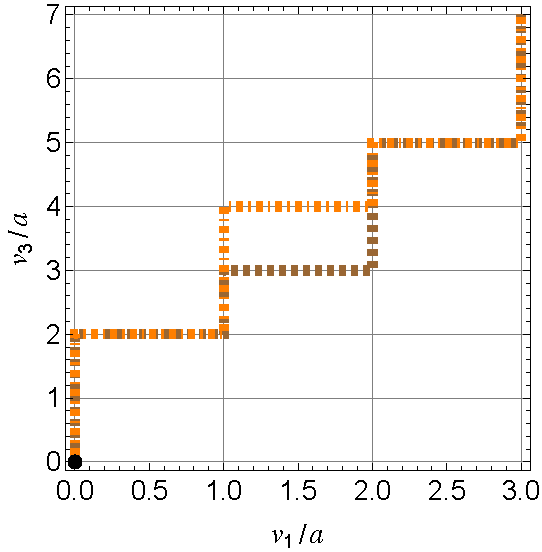
\includegraphics[width=0.85\linewidth]{Example_v_plot_with_2path.pdf}\\
      {\scriptsize Two degenerate paths (solid, dashed) to the same site are averaged.}
    \end{column}
  \end{columns}
\end{frame}

% Slide 27
\begin{frame}{Interpolation to the off-axis direction}
  \begin{columns}[c]
    \begin{column}{0.30\textwidth}
      \[ \Delta v_1 = \frac{v_1^{\text{constraint}} - v_1^{\text{lattice}}}{a} \]
      \begin{itemize}
        \item Path-averaged correlators at three or more bounding sites (red).
        \item Quadratic interpolation in $\Delta v_1$ inside each Jackknife (leave-one-out resampling) sample (grey band).
        \item Read off the value at $\Delta v_1 = 0$ (blue).
        \item All 8 inputs: Re and Im of $R_{\Gamma}$ for $\Gamma=\gamma_1,\gamma_2,\gamma_3,\gamma_4$.
      \end{itemize}
      {\scriptsize $\vect{b}=(1,2,0)$, $\eta=7$, $P_L=-1$}
    \end{column}
    \begin{column}{0.70\textwidth}
      \centering
      \begin{tabular}{@{}c@{\hspace{1mm}}c@{}}
        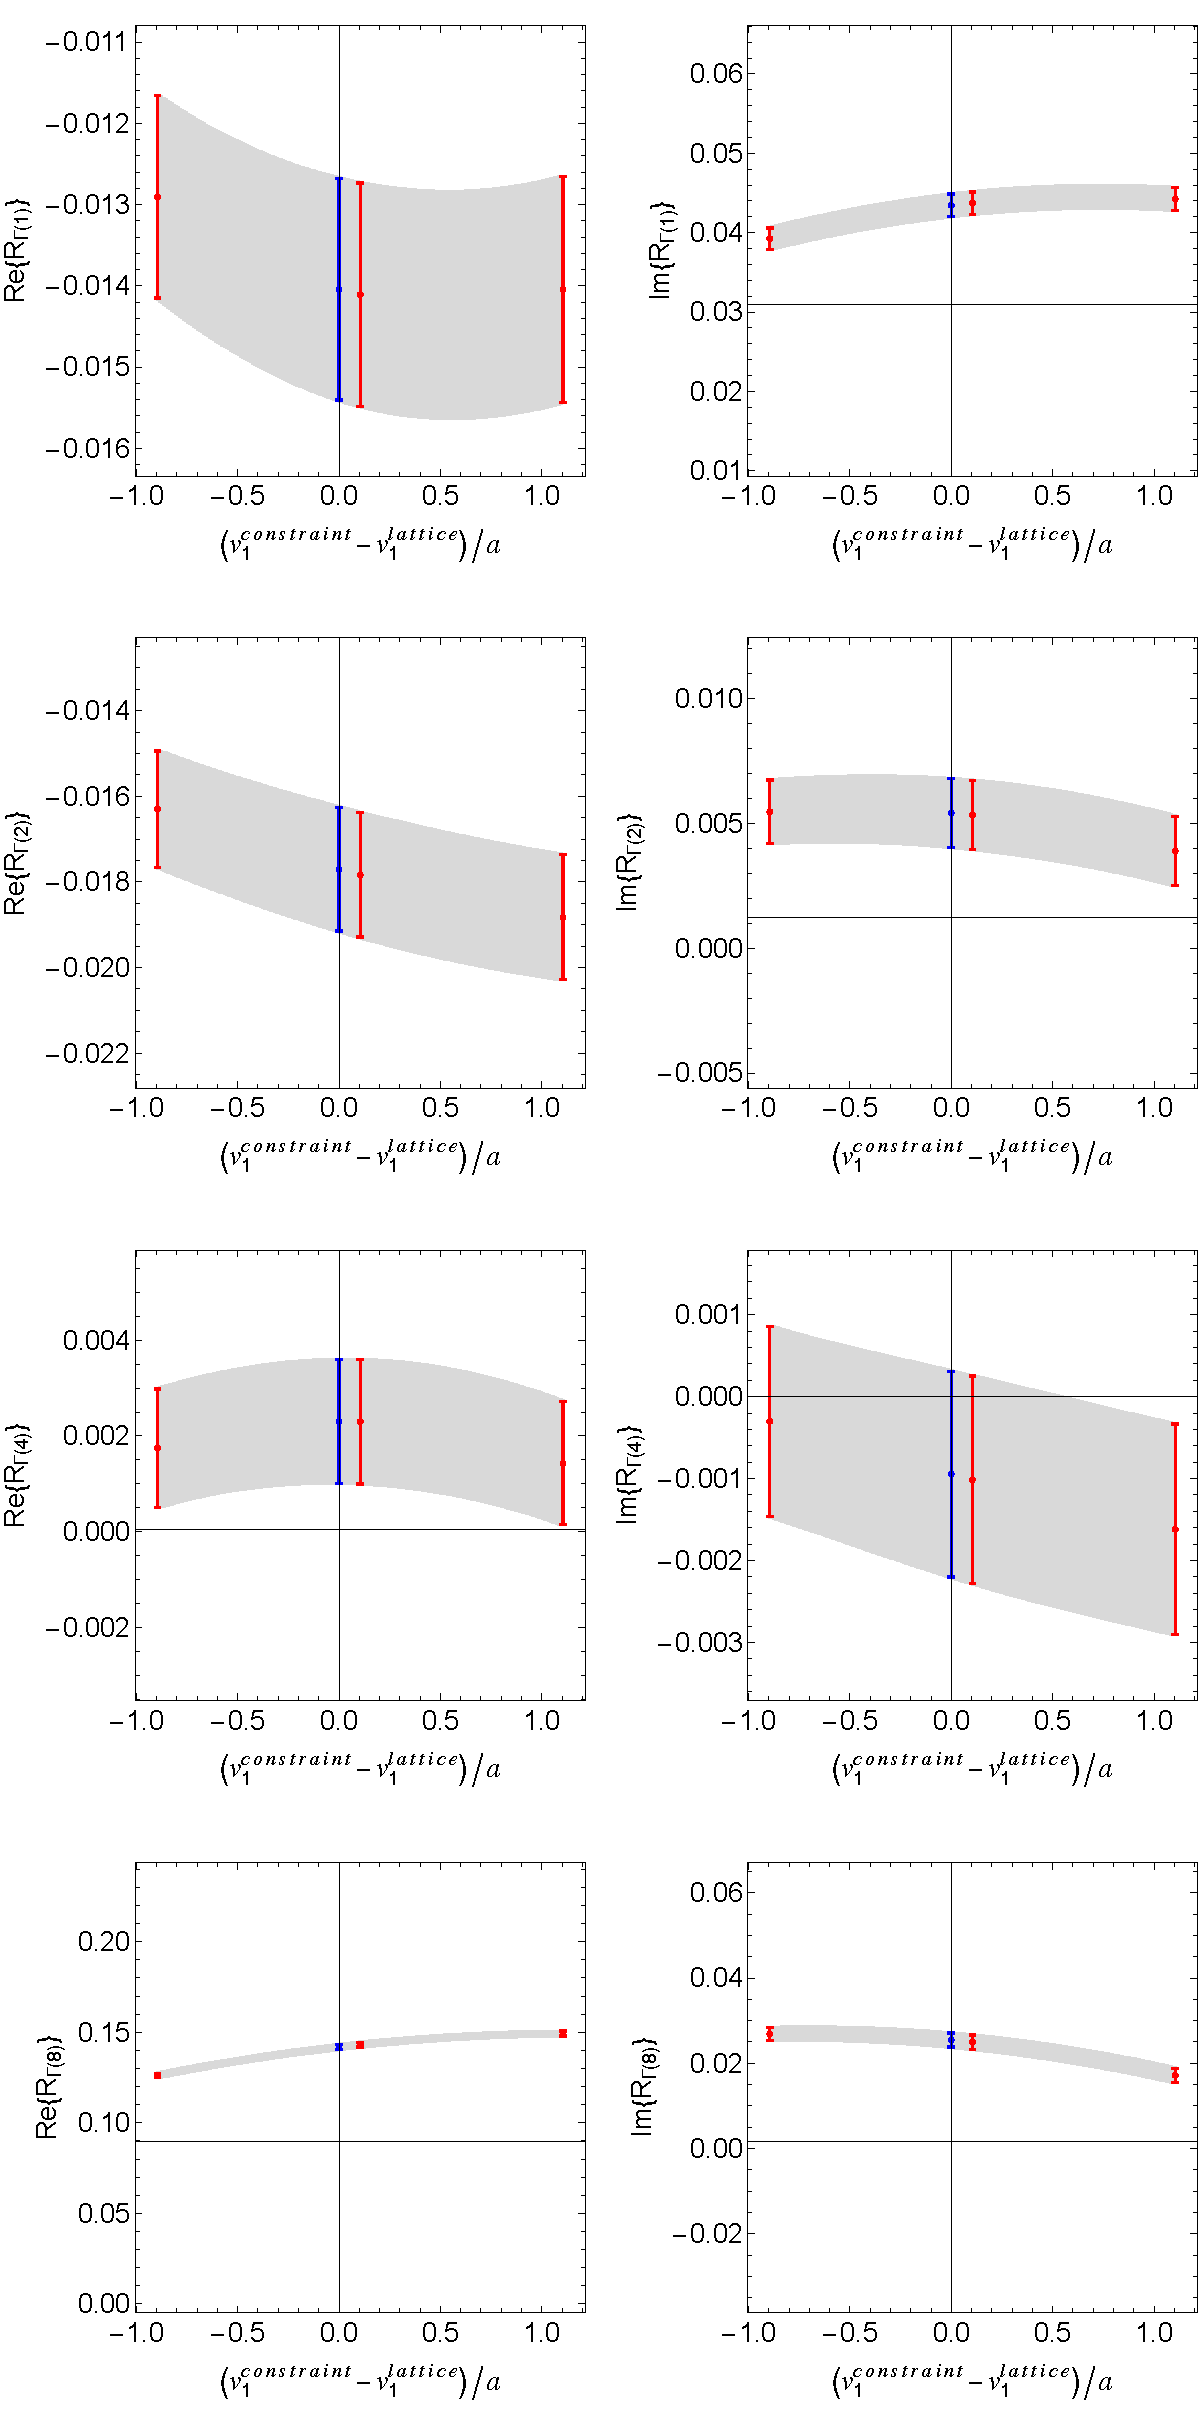
\includegraphics[height=0.6\textheight, trim=0 582 0 0, clip]{Interpolation_Ex_b120_eta7_P-1.pdf} &
        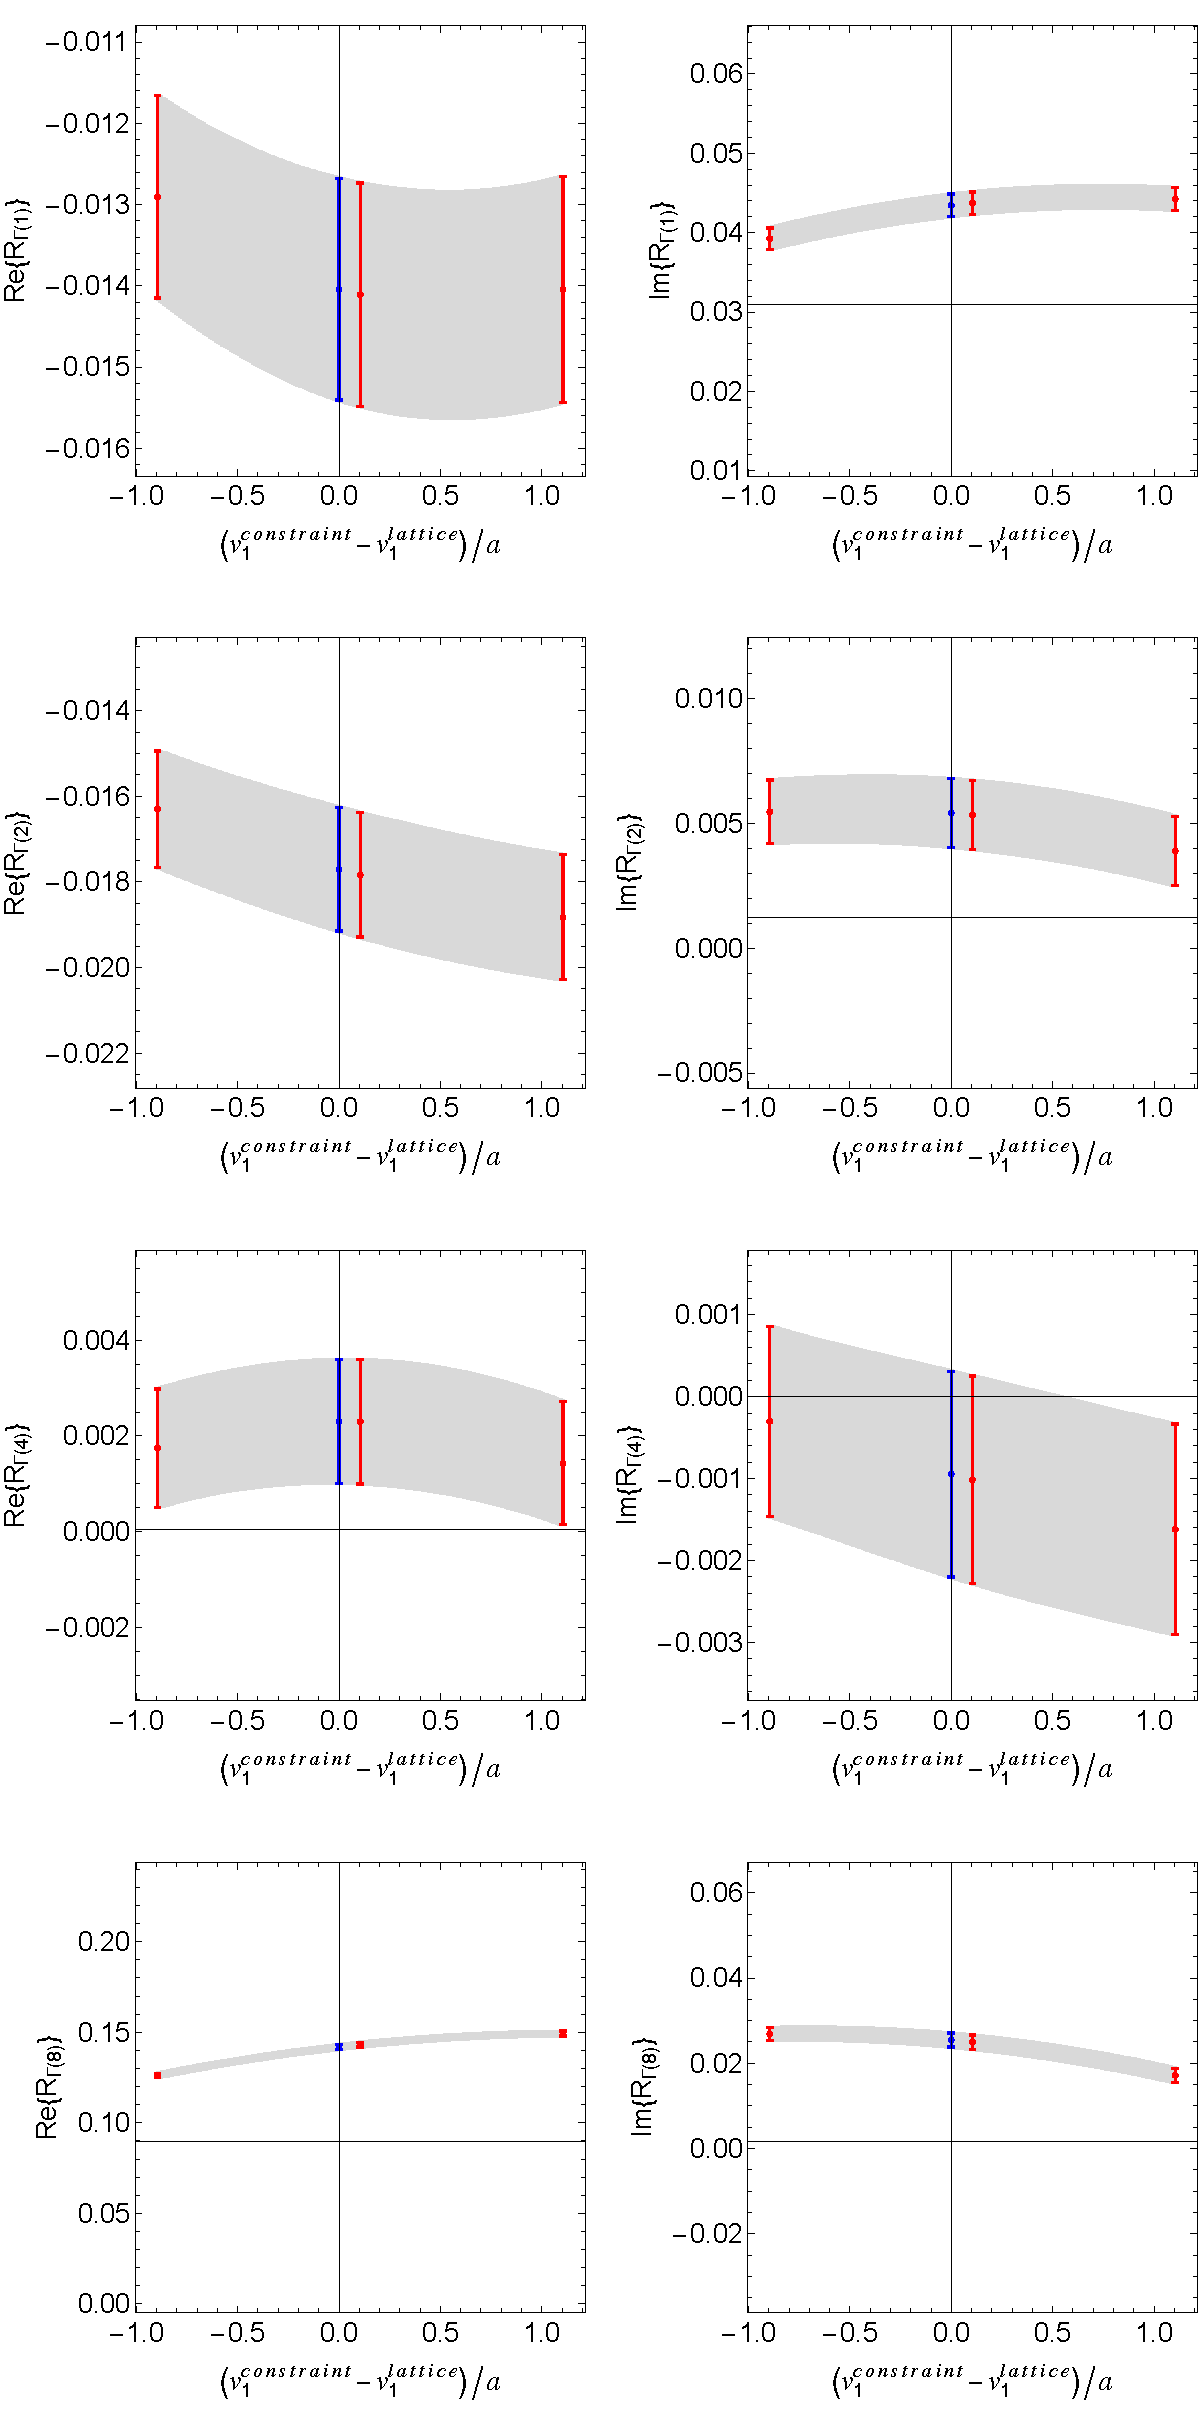
\includegraphics[height=0.6\textheight, trim=0 0 0 582, clip]{Interpolation_Ex_b120_eta7_P-1.pdf} \\
        {\scriptsize $\Gamma=\gamma_1,\gamma_2$: Re (left), Im (right)} & {\scriptsize $\Gamma=\gamma_3,\gamma_4$: Re (left), Im (right)}
      \end{tabular}
    \end{column}
  \end{columns}
\end{frame}

% Slide 28
\begin{frame}{Quark separation vectors $\vect b$}
  \begin{columns}[c]
    \begin{column}{0.4\textwidth}
      \centering
      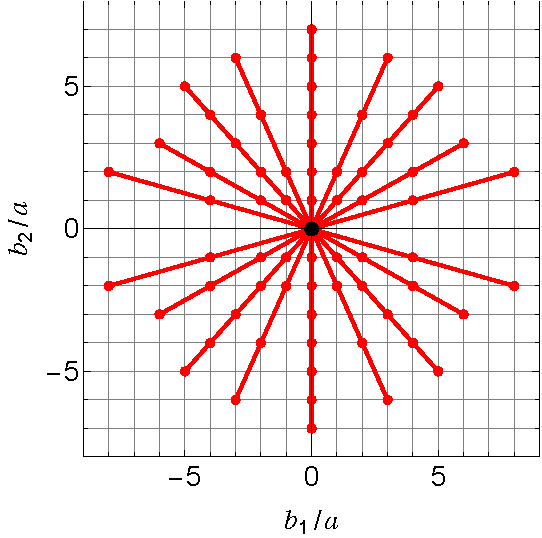
\includegraphics[width=0.9\linewidth]{bL_bT_plot.pdf}\\
      {\scriptsize Sampled $\vect b$ in the $b_1$--$b_2$ plane ($b_1\equiv b_L$, $b_2\equiv b_T$)}
    \end{column}
    \begin{column}{0.58\textwidth}
      \centering
      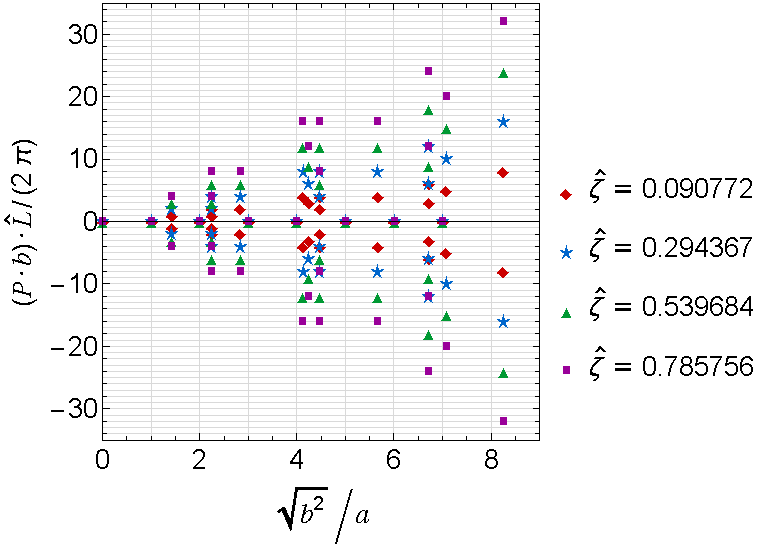
\includegraphics[width=0.95\linewidth]{Pb_bsq_plot.pdf}\\
      {\scriptsize The same vectors in $(\bvec\tcdot P,\ |\vect b|)$ for the four $\zetahat$}
    \end{column}
  \end{columns}
  \begin{itemize}
    \item $P$ along $\hat x_1$: \ $\bvec\cdot P=-P_1 b_1$. Each $+b_1$ has a mirrored $-b_1$, so we reach $\pm\bvec\tcdot P$.
    \item Higher $|P_L|$ stretches the reach in $\bvec\tcdot P$.
  \end{itemize}
\end{frame}

\begin{frame}{Quark-separation path pairs: table 1, part 1}
\label{coverage:bpaths-1-1}
\centering\small
\begin{tabular}{l@{\hspace{12mm}}l}
Coordinate $(b_1,b_2,b_3)/a$ & Reflected coordinate $(-b_1,b_2,b_3)/a$\\\hline
$\{0,0,0\}$ & $\{0,0,0\}$\\
$\{\}$ & $\{\}$\\
\noalign{\vskip3pt}
$\{0,1,0\}$ & $\{0,1,0\}$\\
$\{2\}$ & $\{2\}$\\
\noalign{\vskip3pt}
$\{0,2,0\}$ & $\{0,2,0\}$\\
$\{2,2\}$ & $\{2,2\}$\\
\noalign{\vskip3pt}
$\{0,3,0\}$ & $\{0,3,0\}$\\
$\{2,2,2\}$ & $\{2,2,2\}$\\
\noalign{\vskip3pt}
\end{tabular}
\figsrc{Thesis, Ch. 5: original path entries; a signed integer denotes a directed lattice step.}
\end{frame}

\begin{frame}{Quark-separation path pairs: table 1, part 2}
\label{coverage:bpaths-1-2}
\centering\small
\begin{tabular}{l@{\hspace{12mm}}l}
Coordinate $(b_1,b_2,b_3)/a$ & Reflected coordinate $(-b_1,b_2,b_3)/a$\\\hline
$\{0,4,0\}$ & $\{0,4,0\}$\\
$\{2,2,2,2\}$ & $\{2,2,2,2\}$\\
\noalign{\vskip3pt}
$\{0,5,0\}$ & $\{0,5,0\}$\\
$\{2,2,2,2,2\}$ & $\{2,2,2,2,2\}$\\
\noalign{\vskip3pt}
$\{0,6,0\}$ & $\{0,6,0\}$\\
$\{2,2,2,2,2,2\}$ & $\{2,2,2,2,2,2\}$\\
\noalign{\vskip3pt}
$\{0,7,0\}$ & $\{0,7,0\}$\\
$\{2,2,2,2,2,2,2\}$ & $\{2,2,2,2,2,2,2\}$\\
\noalign{\vskip3pt}
\end{tabular}
\figsrc{Thesis, Ch. 5: original path entries; a signed integer denotes a directed lattice step.}
\end{frame}

\begin{frame}{Quark-separation path pairs: table 1, part 3}
\label{coverage:bpaths-1-3}
\centering\small
\begin{tabular}{l@{\hspace{12mm}}l}
Coordinate $(b_1,b_2,b_3)/a$ & Reflected coordinate $(-b_1,b_2,b_3)/a$\\\hline
$\{0,-1,0\}$ & $\{0,-1,0\}$\\
$\{-2\}$ & $\{-2\}$\\
\noalign{\vskip3pt}
$\{0,-2,0\}$ & $\{0,-2,0\}$\\
$\{-2,-2\}$ & $\{-2,-2\}$\\
\noalign{\vskip3pt}
$\{0,-3,0\}$ & $\{0,-3,0\}$\\
$\{-2,-2,-2\}$ & $\{-2,-2,-2\}$\\
\noalign{\vskip3pt}
$\{0,-4,0\}$ & $\{0,-4,0\}$\\
$\{-2,-2,-2,-2\}$ & $\{-2,-2,-2,-2\}$\\
\noalign{\vskip3pt}
\end{tabular}
\figsrc{Thesis, Ch. 5: original path entries; a signed integer denotes a directed lattice step.}
\end{frame}

\begin{frame}{Quark-separation path pairs: table 1, part 4}
\label{coverage:bpaths-1-4}
\centering\small
\begin{tabular}{l@{\hspace{12mm}}l}
Coordinate $(b_1,b_2,b_3)/a$ & Reflected coordinate $(-b_1,b_2,b_3)/a$\\\hline
$\{0,-5,0\}$ & $\{0,-5,0\}$\\
$\{-2,-2,-2,-2,-2\}$ & $\{-2,-2,-2,-2,-2\}$\\
\noalign{\vskip3pt}
$\{0,-6,0\}$ & $\{0,-6,0\}$\\
$\{-2,-2,-2,-2,-2,-2\}$ & $\{-2,-2,-2,-2,-2,-2\}$\\
\noalign{\vskip3pt}
$\{0,-7,0\}$ & $\{0,-7,0\}$\\
$\{-2,-2,-2,-2,-2,-2,-2\}$ & $\{-2,-2,-2,-2,-2,-2,-2\}$\\
\noalign{\vskip3pt}
\end{tabular}
\figsrc{Thesis, Ch. 5: original path entries; a signed integer denotes a directed lattice step.}
\end{frame}

\begin{frame}{Quark-separation path pairs: table 2, part 1}
\label{coverage:bpaths-2-1}
\centering\small
\begin{tabular}{l@{\hspace{12mm}}l}
Coordinate $(b_1,b_2,b_3)/a$ & Reflected coordinate $(-b_1,b_2,b_3)/a$\\\hline
$\{1,1,0\}$ & $\{-1,1,0\}$\\
$\{2,1\}$ & $\{2,-1\}$\\
$\{1,2\}$ & $\{-1,2\}$\\
\noalign{\vskip3pt}
$\{2,2,0\}$ & $\{-2,2,0\}$\\
$\{2,1,2,1\}$ & $\{2,-1,2,-1\}$\\
$\{1,2,1,2\}$ & $\{-1,2,-1,2\}$\\
\noalign{\vskip3pt}
$\{3,3,0\}$ & $\{-3,3,0\}$\\
$\{2,1,2,1,2,1\}$ & $\{2,-1,2,-1,2,-1\}$\\
$\{1,2,1,2,1,2\}$ & $\{-1,2,-1,2,-1,2\}$\\
\noalign{\vskip3pt}
$\{4,4,0\}$ & $\{-4,4,0\}$\\
$\{2,1,2,1,2,1,2,1\}$ & $\{2,-1,2,-1,2,-1,2,-1\}$\\
$\{1,2,1,2,1,2,1,2\}$ & $\{-1,2,-1,2,-1,2,-1,2\}$\\
\noalign{\vskip3pt}
\end{tabular}
\figsrc{Thesis, Ch. 5: original path entries; a signed integer denotes a directed lattice step.}
\end{frame}

\begin{frame}{Quark-separation path pairs: table 2, part 2}
\label{coverage:bpaths-2-2}
\centering\small
\begin{tabular}{l@{\hspace{12mm}}l}
Coordinate $(b_1,b_2,b_3)/a$ & Reflected coordinate $(-b_1,b_2,b_3)/a$\\\hline
$\{5,5,0\}$ & $\{-5,5,0\}$\\
$\{2,1,2,1,2,1,2,1,2,1\}$ & $\{2,-1,2,-1,2,-1,2,-1,2,-1\}$\\
$\{1,2,1,2,1,2,1,2,1,2\}$ & $\{-1,2,-1,2,-1,2,-1,2,-1,2\}$\\
\noalign{\vskip3pt}
$\{1,2,0\}$ & $\{-1,2,0\}$\\
$\{2,1,2\}$ & $\{2,-1,2\}$\\
\noalign{\vskip3pt}
$\{2,4,0\}$ & $\{-2,4,0\}$\\
$\{2,1,2,2,1,2\}$ & $\{2,-1,2,2,-1,2\}$\\
\noalign{\vskip3pt}
$\{3,6,0\}$ & $\{-3,6,0\}$\\
$\{2,1,2,2,1,2,2,1,2\}$ & $\{2,-1,2,2,-1,2,2,-1,2\}$\\
\noalign{\vskip3pt}
\end{tabular}
\figsrc{Thesis, Ch. 5: original path entries; a signed integer denotes a directed lattice step.}
\end{frame}

\begin{frame}{Quark-separation path pairs: table 2, part 3}
\label{coverage:bpaths-2-3}
\centering\small
\begin{tabular}{l@{\hspace{12mm}}l}
Coordinate $(b_1,b_2,b_3)/a$ & Reflected coordinate $(-b_1,b_2,b_3)/a$\\\hline
$\{2,1,0\}$ & $\{-2,1,0\}$\\
$\{1,2,1\}$ & $\{-1,2,-1\}$\\
\noalign{\vskip3pt}
$\{4,2,0\}$ & $\{-4,2,0\}$\\
$\{1,2,1,1,2,1\}$ & $\{-1,2,-1,-1,2,-1\}$\\
\noalign{\vskip3pt}
$\{6,3,0\}$ & $\{-6,3,0\}$\\
$\{1,2,1,1,2,1,1,2,1\}$ & $\{-1,2,-1,-1,2,-1,-1,2,-1\}$\\
\noalign{\vskip3pt}
$\{4,1,0\}$ & $\{-4,1,0\}$\\
$\{1,1,2,1,1\}$ & $\{-1,-1,2,-1,-1\}$\\
\noalign{\vskip3pt}
\end{tabular}
\figsrc{Thesis, Ch. 5: original path entries; a signed integer denotes a directed lattice step.}
\end{frame}

\begin{frame}{Quark-separation path pairs: table 2, part 4}
\label{coverage:bpaths-2-4}
\centering\small
\begin{tabular}{l@{\hspace{12mm}}l}
Coordinate $(b_1,b_2,b_3)/a$ & Reflected coordinate $(-b_1,b_2,b_3)/a$\\\hline
$\{8,2,0\}$ & $\{-8,2,0\}$\\
$\{1,1,2,1,1,1,1,2,1,1\}$ & $\{-1,-1,2,-1,-1,-1,-1,2,-1,-1\}$\\
\noalign{\vskip3pt}
$\{1,-1,0\}$ & $\{-1,-1,0\}$\\
$\{-2,1\}$ & $\{-2,-1\}$\\
$\{1,-2\}$ & $\{-1,-2\}$\\
\noalign{\vskip3pt}
$\{2,-2,0\}$ & $\{-2,-2,0\}$\\
$\{-2,1,-2,1\}$ & $\{-2,-1,-2,-1\}$\\
$\{1,-2,1,-2\}$ & $\{-1,-2,-1,-2\}$\\
\noalign{\vskip3pt}
$\{3,-3,0\}$ & $\{-3,-3,0\}$\\
$\{-2,1,-2,1,-2,1\}$ & $\{-2,-1,-2,-1,-2,-1\}$\\
$\{1,-2,1,-2,1,-2\}$ & $\{-1,-2,-1,-2,-1,-2\}$\\
\noalign{\vskip3pt}
\end{tabular}
\figsrc{Thesis, Ch. 5: original path entries; a signed integer denotes a directed lattice step.}
\end{frame}

\begin{frame}{Quark-separation path pairs: table 2, part 5}
\label{coverage:bpaths-2-5}
\centering\small
\begin{tabular}{l@{\hspace{12mm}}l}
Coordinate $(b_1,b_2,b_3)/a$ & Reflected coordinate $(-b_1,b_2,b_3)/a$\\\hline
$\{4,-4,0\}$ & $\{-4,-4,0\}$\\
$\{-2,1,-2,1,-2,1,-2,1\}$ & $\{-2,-1,-2,-1,-2,-1,-2,-1\}$\\
$\{1,-2,1,-2,1,-2,1,-2\}$ & $\{-1,-2,-1,-2,-1,-2,-1,-2\}$\\
\noalign{\vskip3pt}
$\{5,-5,0\}$ & $\{-5,-5,0\}$\\
$\{-2,1,-2,1,-2,1,-2,1,-2,1\}$ & $\{-2,-1,-2,-1,-2,-1,-2,-1,-2,-1\}$\\
$\{1,-2,1,-2,1,-2,1,-2,1,-2\}$ & $\{-1,-2,-1,-2,-1,-2,-1,-2,-1,-2\}$\\
\noalign{\vskip3pt}
$\{1,-2,0\}$ & $\{-1,-2,0\}$\\
$\{-2,1,-2\}$ & $\{-2,-1,-2\}$\\
\noalign{\vskip3pt}
$\{2,-4,0\}$ & $\{-2,-4,0\}$\\
$\{-2,1,-2,-2,1,-2\}$ & $\{-2,-1,-2,-2,-1,-2\}$\\
\noalign{\vskip3pt}
\end{tabular}
\figsrc{Thesis, Ch. 5: original path entries; a signed integer denotes a directed lattice step.}
\end{frame}

\begin{frame}{Quark-separation path pairs: table 2, part 6}
\label{coverage:bpaths-2-6}
\centering\small
\begin{tabular}{l@{\hspace{12mm}}l}
Coordinate $(b_1,b_2,b_3)/a$ & Reflected coordinate $(-b_1,b_2,b_3)/a$\\\hline
$\{3,-6,0\}$ & $\{-3,-6,0\}$\\
$\{-2,1,-2,-2,1,-2,-2,1,-2\}$ & $\{-2,-1,-2,-2,-1,-2,-2,-1,-2\}$\\
\noalign{\vskip3pt}
$\{2,-1,0\}$ & $\{-2,-1,0\}$\\
$\{1,-2,1\}$ & $\{-1,-2,-1\}$\\
\noalign{\vskip3pt}
$\{4,-2,0\}$ & $\{-4,-2,0\}$\\
$\{1,-2,1,1,-2,1\}$ & $\{-1,-2,-1,-1,-2,-1\}$\\
\noalign{\vskip3pt}
$\{6,-3,0\}$ & $\{-6,-3,0\}$\\
$\{1,-2,1,1,-2,1,1,-2,1\}$ & $\{-1,-2,-1,-1,-2,-1,-1,-2,-1\}$\\
\noalign{\vskip3pt}
\end{tabular}
\figsrc{Thesis, Ch. 5: original path entries; a signed integer denotes a directed lattice step.}
\end{frame}

\begin{frame}{Quark-separation path pairs: table 2, part 7}
\label{coverage:bpaths-2-7}
\centering\small
\begin{tabular}{l@{\hspace{12mm}}l}
Coordinate $(b_1,b_2,b_3)/a$ & Reflected coordinate $(-b_1,b_2,b_3)/a$\\\hline
$\{4,-1,0\}$ & $\{-4,-1,0\}$\\
$\{1,1,-2,1,1\}$ & $\{-1,-1,-2,-1,-1\}$\\
\noalign{\vskip3pt}
$\{8,-2,0\}$ & $\{-8,-2,0\}$\\
$\{1,1,-2,1,1,1,1,-2,1,1\}$ & $\{-1,-1,-2,-1,-1,-1,-1,-2,-1,-1\}$\\
\noalign{\vskip3pt}
\end{tabular}
\figsrc{Thesis, Ch. 5: original path entries; a signed integer denotes a directed lattice step.}
\end{frame}

\begin{frame}{Quark-separation path pairs: table 3, part 1}
\label{coverage:bpaths-3-1}
\centering\small
\begin{tabular}{l@{\hspace{12mm}}l}
Coordinate $(b_1,b_2,b_3)/a$ & Reflected coordinate $(-b_1,b_2,b_3)/a$\\\hline
$\{-1,1,0\}$ & $\{1,1,0\}$\\
$\{2,-1\}$ & $\{2,1\}$\\
$\{-1,2\}$ & $\{1,2\}$\\
\noalign{\vskip3pt}
$\{-2,2,0\}$ & $\{2,2,0\}$\\
$\{2,-1,2,-1\}$ & $\{2,1,2,1\}$\\
$\{-1,2,-1,2\}$ & $\{1,2,1,2\}$\\
\noalign{\vskip3pt}
$\{-3,3,0\}$ & $\{3,3,0\}$\\
$\{2,-1,2,-1,2,-1\}$ & $\{2,1,2,1,2,1\}$\\
$\{-1,2,-1,2,-1,2\}$ & $\{1,2,1,2,1,2\}$\\
\noalign{\vskip3pt}
$\{-4,4,0\}$ & $\{4,4,0\}$\\
$\{2,-1,2,-1,2,-1,2,-1\}$ & $\{2,1,2,1,2,1,2,1\}$\\
$\{-1,2,-1,2,-1,2,-1,2\}$ & $\{1,2,1,2,1,2,1,2\}$\\
\noalign{\vskip3pt}
\end{tabular}
\figsrc{Thesis, Ch. 5: original path entries; a signed integer denotes a directed lattice step.}
\end{frame}

\begin{frame}{Quark-separation path pairs: table 3, part 2}
\label{coverage:bpaths-3-2}
\centering\small
\begin{tabular}{l@{\hspace{12mm}}l}
Coordinate $(b_1,b_2,b_3)/a$ & Reflected coordinate $(-b_1,b_2,b_3)/a$\\\hline
$\{-5,5,0\}$ & $\{5,5,0\}$\\
$\{2,-1,2,-1,2,-1,2,-1,2,-1\}$ & $\{2,1,2,1,2,1,2,1,2,1\}$\\
$\{-1,2,-1,2,-1,2,-1,2,-1,2\}$ & $\{1,2,1,2,1,2,1,2,1,2\}$\\
\noalign{\vskip3pt}
$\{-1,2,0\}$ & $\{1,2,0\}$\\
$\{2,-1,2\}$ & $\{2,1,2\}$\\
\noalign{\vskip3pt}
$\{-2,4,0\}$ & $\{2,4,0\}$\\
$\{2,-1,2,2,-1,2\}$ & $\{2,1,2,2,1,2\}$\\
\noalign{\vskip3pt}
$\{-3,6,0\}$ & $\{3,6,0\}$\\
$\{2,-1,2,2,-1,2,2,-1,2\}$ & $\{2,1,2,2,1,2,2,1,2\}$\\
\noalign{\vskip3pt}
\end{tabular}
\figsrc{Thesis, Ch. 5: original path entries; a signed integer denotes a directed lattice step.}
\end{frame}

\begin{frame}{Quark-separation path pairs: table 3, part 3}
\label{coverage:bpaths-3-3}
\centering\small
\begin{tabular}{l@{\hspace{12mm}}l}
Coordinate $(b_1,b_2,b_3)/a$ & Reflected coordinate $(-b_1,b_2,b_3)/a$\\\hline
$\{-2,1,0\}$ & $\{2,1,0\}$\\
$\{-1,2,-1\}$ & $\{1,2,1\}$\\
\noalign{\vskip3pt}
$\{-4,2,0\}$ & $\{4,2,0\}$\\
$\{-1,2,-1,-1,2,-1\}$ & $\{1,2,1,1,2,1\}$\\
\noalign{\vskip3pt}
$\{-6,3,0\}$ & $\{6,3,0\}$\\
$\{-1,2,-1,-1,2,-1,-1,2,-1\}$ & $\{1,2,1,1,2,1,1,2,1\}$\\
\noalign{\vskip3pt}
$\{-4,1,0\}$ & $\{4,1,0\}$\\
$\{-1,-1,2,-1,-1\}$ & $\{1,1,2,1,1\}$\\
\noalign{\vskip3pt}
\end{tabular}
\figsrc{Thesis, Ch. 5: original path entries; a signed integer denotes a directed lattice step.}
\end{frame}

\begin{frame}{Quark-separation path pairs: table 3, part 4}
\label{coverage:bpaths-3-4}
\centering\small
\begin{tabular}{l@{\hspace{12mm}}l}
Coordinate $(b_1,b_2,b_3)/a$ & Reflected coordinate $(-b_1,b_2,b_3)/a$\\\hline
$\{-8,2,0\}$ & $\{8,2,0\}$\\
$\{-1,-1,2,-1,-1,-1,-1,2,-1,-1\}$ & $\{1,1,2,1,1,1,1,2,1,1\}$\\
\noalign{\vskip3pt}
$\{-1,-1,0\}$ & $\{1,-1,0\}$\\
$\{-2,-1\}$ & $\{-2,1\}$\\
$\{-1,-2\}$ & $\{1,-2\}$\\
\noalign{\vskip3pt}
$\{-2,-2,0\}$ & $\{2,-2,0\}$\\
$\{-2,-1,-2,-1\}$ & $\{-2,1,-2,1\}$\\
$\{-1,-2,-1,-2\}$ & $\{1,-2,1,-2\}$\\
\noalign{\vskip3pt}
$\{-3,-3,0\}$ & $\{3,-3,0\}$\\
$\{-2,-1,-2,-1,-2,-1\}$ & $\{-2,1,-2,1,-2,1\}$\\
$\{-1,-2,-1,-2,-1,-2\}$ & $\{1,-2,1,-2,1,-2\}$\\
\noalign{\vskip3pt}
\end{tabular}
\figsrc{Thesis, Ch. 5: original path entries; a signed integer denotes a directed lattice step.}
\end{frame}

\begin{frame}{Quark-separation path pairs: table 3, part 5}
\label{coverage:bpaths-3-5}
\centering\small
\begin{tabular}{l@{\hspace{12mm}}l}
Coordinate $(b_1,b_2,b_3)/a$ & Reflected coordinate $(-b_1,b_2,b_3)/a$\\\hline
$\{-4,-4,0\}$ & $\{4,-4,0\}$\\
$\{-2,-1,-2,-1,-2,-1,-2,-1\}$ & $\{-2,1,-2,1,-2,1,-2,1\}$\\
$\{-1,-2,-1,-2,-1,-2,-1,-2\}$ & $\{1,-2,1,-2,1,-2,1,-2\}$\\
\noalign{\vskip3pt}
$\{-5,-5,0\}$ & $\{5,-5,0\}$\\
$\{-2,-1,-2,-1,-2,-1,-2,-1,-2,-1\}$ & $\{-2,1,-2,1,-2,1,-2,1,-2,1\}$\\
$\{-1,-2,-1,-2,-1,-2,-1,-2,-1,-2\}$ & $\{1,-2,1,-2,1,-2,1,-2,1,-2\}$\\
\noalign{\vskip3pt}
$\{-1,-2,0\}$ & $\{1,-2,0\}$\\
$\{-2,-1,-2\}$ & $\{-2,1,-2\}$\\
\noalign{\vskip3pt}
$\{-2,-4,0\}$ & $\{2,-4,0\}$\\
$\{-2,-1,-2,-2,-1,-2\}$ & $\{-2,1,-2,-2,1,-2\}$\\
\noalign{\vskip3pt}
\end{tabular}
\figsrc{Thesis, Ch. 5: original path entries; a signed integer denotes a directed lattice step.}
\end{frame}

\begin{frame}{Quark-separation path pairs: table 3, part 6}
\label{coverage:bpaths-3-6}
\centering\small
\begin{tabular}{l@{\hspace{12mm}}l}
Coordinate $(b_1,b_2,b_3)/a$ & Reflected coordinate $(-b_1,b_2,b_3)/a$\\\hline
$\{-3,-6,0\}$ & $\{3,-6,0\}$\\
$\{-2,-1,-2,-2,-1,-2,-2,-1,-2\}$ & $\{-2,1,-2,-2,1,-2,-2,1,-2\}$\\
\noalign{\vskip3pt}
$\{-2,-1,0\}$ & $\{2,-1,0\}$\\
$\{-1,-2,-1\}$ & $\{1,-2,1\}$\\
\noalign{\vskip3pt}
$\{-4,-2,0\}$ & $\{4,-2,0\}$\\
$\{-1,-2,-1,-1,-2,-1\}$ & $\{1,-2,1,1,-2,1\}$\\
\noalign{\vskip3pt}
$\{-6,-3,0\}$ & $\{6,-3,0\}$\\
$\{-1,-2,-1,-1,-2,-1,-1,-2,-1\}$ & $\{1,-2,1,1,-2,1,1,-2,1\}$\\
\noalign{\vskip3pt}
\end{tabular}
\figsrc{Thesis, Ch. 5: original path entries; a signed integer denotes a directed lattice step.}
\end{frame}

\begin{frame}{Quark-separation path pairs: table 3, part 7}
\label{coverage:bpaths-3-7}
\centering\small
\begin{tabular}{l@{\hspace{12mm}}l}
Coordinate $(b_1,b_2,b_3)/a$ & Reflected coordinate $(-b_1,b_2,b_3)/a$\\\hline
$\{-4,-1,0\}$ & $\{4,-1,0\}$\\
$\{-1,-1,-2,-1,-1\}$ & $\{1,1,-2,1,1\}$\\
\noalign{\vskip3pt}
$\{-8,-2,0\}$ & $\{8,-2,0\}$\\
$\{-1,-1,-2,-1,-1,-1,-1,-2,-1,-1\}$ & $\{1,1,-2,1,1,1,1,-2,1,1\}$\\
\noalign{\vskip3pt}
\end{tabular}
\figsrc{Thesis, Ch. 5: original path entries; a signed integer denotes a directed lattice step.}
\end{frame}


% Slide 30
\begin{frame}{Symmetry improvement: path averaging for $\vect b$}
  \quick
  \begin{columns}[c]
    \begin{column}{0.48\textwidth}
      \centering
      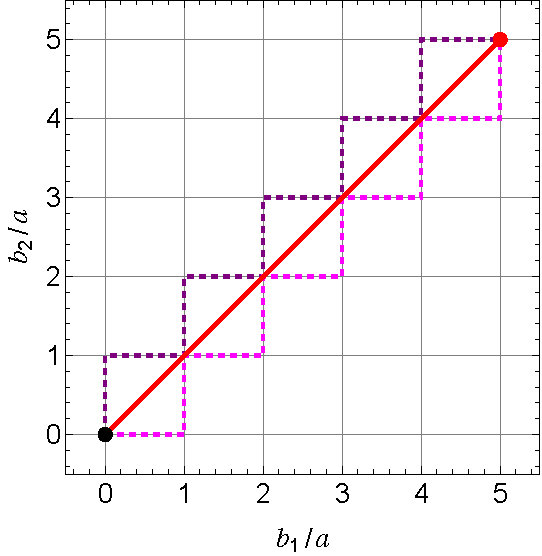
\includegraphics[width=0.85\linewidth]{Example_b_plot_with_2path.pdf}\\
      {\scriptsize Degenerate paths to the same $\vect b$ (solid, dashed) are averaged.}
    \end{column}
    \begin{column}{0.48\textwidth}
      \centering
      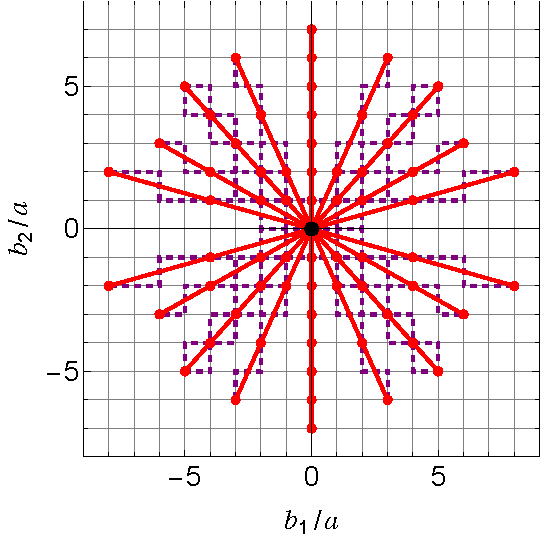
\includegraphics[width=0.85\linewidth]{bL_bT_plot_with_path.pdf}\\
      {\scriptsize Full network: ideal vectors (solid red), averaged staircase paths (dashed)}
    \end{column}
  \end{columns}
  \begin{itemize}
    \item Same operation as for $v$: average over all step-wise paths sharing origin and endpoint.
  \end{itemize}
\end{frame}

% Slide 31
% ===== Correlator decomposition: all four Dirac structures, +b / -b, even / odd (follows thesis, Extracting the x-dependence) =====
\newcommand{\En}{E_N}
\newcommand{\Pa}{|\vec P^{1}|}
\newcommand{\aR}[1]{\tilde a^{\text{Re}}_{#1}}
\newcommand{\aI}[1]{\tilde a^{\text{Im}}_{#1}}
\newcommand{\bR}[1]{\tilde b^{\text{Re}}_{#1}}
\newcommand{\bI}[1]{\tilde b^{\text{Im}}_{#1}}
\newcommand{\Rr}[3]{\text{#1}\{R_{\Gamma(#2)}\}^{[#3]}}
\newcommand{\fl}{\textcolor{red}}

\begin{frame}{Dirac structures $\Gamma$: Euclidean (lattice) versus Minkowski}
  \begin{itemize}
    \item The lattice code uses Euclidean $\gamma_E$; the amplitudes are defined with Minkowski $\gamma_M$:
  \end{itemize}
  \[ \gamma^{1}_{E}=+i\gamma^{1}_{M},\quad \gamma^{2}_{E}=-i\gamma^{2}_{M},\quad \gamma^{3}_{E}=+i\gamma^{3}_{M},\quad \gamma^{4}_{E}=\gamma^{0}_{M},\quad \gamma^{5}_{E}=\gamma^{1}_{E}\gamma^{2}_{E}\gamma^{3}_{E}\gamma^{4}_{E}=-\gamma^{5}_{M} \]
  \begin{itemize}
    \item The index $i\in\{1,2,4,8\}$ of $\Gamma(i)$ is the bit-encoded position of the structure in the CHROMA/QLUA operator basis:
  \end{itemize}
  \[ \Gamma(1)=[+i\gamma^1],\qquad \Gamma(2)=[-i\gamma^2],\qquad \Gamma(4)=[+i\gamma^3],\qquad \Gamma(8)=[\gamma^0] \]
  \begin{itemize}
    \item Measured: the four ratios $R_{\Gamma(1)},R_{\Gamma(2)},R_{\Gamma(4)},R_{\Gamma(8)}$, each complex, at $(+b^1,b^2,0)$ and $(-b^1,b^2,0)$. Raising spatial indices with $g^{\mu\nu}=\mathrm{diag}(1,-1,-1,-1)$ ($P_1=-P^1$, $b_2=-b^2$), and $P^0\to\En$.
    \item Lattice amplitudes (finite link $\eta$): $\tilde a_i=\tilde a_i^{\text{Re}}+i\tilde a_i^{\text{Im}}$, $\tilde b_i=\tilde b_i^{\text{Re}}+i\tilde b_i^{\text{Im}}$, related to the uppercase parametrization by $\tAmp_i=\tilde a_i$, $\tBmp_i=(\eta v\tcdot P)^n\,\tilde b_i$. Here $n=1$ for $i=1,7,8,9$ and $n=2$ for $i=10$.
  \end{itemize}
  \figsrc{Thesis, Extracting the x-dependence, solving real and imaginary amplitudes.}
\end{frame}

\begin{frame}{Lattice geometry and reflection in $b^1$}
  \[
  P^\mu=(\En,-\Pa,0,0),\quad b^\mu=(0,b^1,b^2,0),
  \quad v^\mu=(0,v^1,0,v^3),\quad S^\mu=(0,0,0,1).
  \]
  \[
  b\cdot S=0,\qquad v\cdot S=-v^3,\qquad v\cdot P=\Pa v^1,
  \qquad \epsilon^{0123}=+1.
  \]
  \begin{itemize}
    \item Reflect only $b^1$, keeping $b^2$, $v$, $P$, $S$ and $\eta$ fixed.
    \item Then $b\cdot P$ and $v\cdot b$ both change sign while $b\cdot b$ stays fixed. Hermiticity gives
  \end{itemize}
  \[
  \tilde a_i[-b^1]=\tilde a_i[+b^1]^*,\qquad
  \tilde b_i[-b^1]=\tilde b_i[+b^1]^*.
  \]
  \begin{itemize}
    \item A spatial component $b^2$ in the following equations means the second Cartesian component. It is distinct from the invariant $b\cdot b$ and the magnitude $|\vect b|^2$.
    \item $\tBmp_9$ vanishes in this geometry because $b\cdot S=0$. The other seven amplitudes remain in the four-channel system.
  \end{itemize}
  \figsrc{Thesis, Extracting the x-dependence, lattice kinematics and amplitude inversion.}
\end{frame}

% ---------------- Gamma(8) = gamma^0 ----------------
\begin{frame}{Correlator for $\Gamma(8)=[\gamma^0]$}
  \small
  Continuum projection (contravariant indices, $S^3$ the nucleon polarization):
  \[ \tfrac12\widetilde\Phi^{[\gamma^0]}_{\unsub}=P^0\,\tAmp_2-i\mN\Pa\,\bvec^2S^3\,\tAmp_{12}-\tfrac{i\mN^3}{v\tcdot P}\,\bvec^2v^1S^3\,\tBmp_8-\tfrac{i\mN^3}{(v\tcdot P)^2}(v\tcdot S)\Pa\,\bvec^2v^3\,\tBmp_{10} \]
  Lattice ratio in terms of the finite-link amplitudes:
  \[ R_{\Gamma(8)}=2\Big[\tilde a_2-i\mN\tfrac{\Pa}{\En}\bvec^2\,\tilde a_{12}-\tfrac{i\mN^3}{\En}\bvec^2\eta v^1\,\tilde b_8+\tfrac{i\mN^3}{\En}\Pa\bvec^2\eta^2(v^3)^2\,\tilde b_{10}\Big] \]
  \figsrc{Thesis, Extracting the x-dependence, projected vector correlator.}
\end{frame}

\begin{frame}{$\Gamma(8)$: the $+b^1$ and $-b^1$ equations}
  \small
  \begin{align*}
    \Rr{Re}{8}{+b^1}&=2\Big[\aR2+\mN\tfrac{\Pa}{\En}\bvec^2\aI{12}+\tfrac{\mN^3}{\En}\bvec^2\eta v^1\bI8-\tfrac{\mN^3}{\En}\Pa\bvec^2\eta^2(v^3)^2\bI{10}\Big]\\
    \Rr{Im}{8}{+b^1}&=2\Big[-\mN\tfrac{\Pa}{\En}\bvec^2\aR{12}-\tfrac{\mN^3}{\En}\bvec^2\eta v^1\bR8+\tfrac{\mN^3}{\En}\Pa\bvec^2\eta^2(v^3)^2\bR{10}+\aI2\Big]\\
    \Rr{Re}{8}{-b^1}&=2\Big[\aR2\fl{-}\mN\tfrac{\Pa}{\En}\bvec^2\aI{12}\fl{-}\tfrac{\mN^3}{\En}\bvec^2\eta v^1\bI8\fl{+}\tfrac{\mN^3}{\En}\Pa\bvec^2\eta^2(v^3)^2\bI{10}\Big]\\
    \Rr{Im}{8}{-b^1}&=2\Big[-\mN\tfrac{\Pa}{\En}\bvec^2\aR{12}-\tfrac{\mN^3}{\En}\bvec^2\eta v^1\bR8+\tfrac{\mN^3}{\En}\Pa\bvec^2\eta^2(v^3)^2\bR{10}\fl{-}\aI2\Big]
  \end{align*}
  {\scriptsize Red: sign flipped relative to $+b^1$, because $\tilde a^{\text{Re}},\tilde b^{\text{Re}}$ are even and $\tilde a^{\text{Im}},\tilde b^{\text{Im}}$ are odd in $b^1$ (and $\bvec^1$ itself flips).}
  \figsrc{Thesis, Extracting the x-dependence, solving real and imaginary amplitudes.}
\end{frame}

% ---------------- Gamma(1) = i gamma^1 ----------------
\begin{frame}{Correlator for $\Gamma(1)=[+i\gamma^1]$}
  \small
  Continuum projection:
  \[ \tfrac12\widetilde\Phi^{[\gamma^1]}_{\unsub}=-\Pa\,\tAmp_2-i\mN^2\bvec^1\tAmp_3+\tfrac{\mN^2}{v\tcdot P}v^1\tBmp_1+i\mN P^0\bvec^2S^3\,\tAmp_{12}+\tfrac{i\mN^3}{(v\tcdot P)^2}(v\tcdot S)P^0\bvec^2v^3\,\tBmp_{10} \]
  Lattice ratio:
  \[ R_{\Gamma(1)}=2\Big[-i\tfrac{\Pa}{\En}\tilde a_2+\tfrac{\mN^2}{\En}\bvec^1\tilde a_3+i\tfrac{\mN^2}{\En}\eta v^1\tilde b_1-\mN\bvec^2\tilde a_{12}+\mN^3\bvec^2\eta^2(v^3)^2\tilde b_{10}\Big] \]
  \figsrc{Thesis, Extracting the x-dependence, projected vector correlator.}
\end{frame}

\begin{frame}{$\Gamma(1)$: the $+b^1$ and $-b^1$ equations}
  \small
  \begin{align*}
    \Rr{Re}{1}{+b^1}&=2\Big[\tfrac{\mN^2}{\En}\bvec^1\aR3-\mN\bvec^2\aR{12}+\mN^3\bvec^2\eta^2(v^3)^2\bR{10}+\tfrac{\Pa}{\En}\aI2-\tfrac{\mN^2}{\En}\eta v^1\bI1\Big]\\
    \Rr{Im}{1}{+b^1}&=2\Big[-\tfrac{\Pa}{\En}\aR2+\tfrac{\mN^2}{\En}\eta v^1\bR1+\tfrac{\mN^2}{\En}\bvec^1\aI3-\mN\bvec^2\aI{12}+\mN^3\bvec^2\eta^2(v^3)^2\bI{10}\Big]\\
    \Rr{Re}{1}{-b^1}&=2\Big[\fl{-}\tfrac{\mN^2}{\En}\bvec^1\aR3-\mN\bvec^2\aR{12}+\mN^3\bvec^2\eta^2(v^3)^2\bR{10}\fl{-}\tfrac{\Pa}{\En}\aI2\fl{+}\tfrac{\mN^2}{\En}\eta v^1\bI1\Big]\\
    \Rr{Im}{1}{-b^1}&=2\Big[-\tfrac{\Pa}{\En}\aR2+\tfrac{\mN^2}{\En}\eta v^1\bR1+\tfrac{\mN^2}{\En}\bvec^1\aI3\fl{+}\mN\bvec^2\aI{12}\fl{-}\mN^3\bvec^2\eta^2(v^3)^2\bI{10}\Big]
  \end{align*}
  \figsrc{Thesis, Extracting the x-dependence, solving real and imaginary amplitudes.}
\end{frame}

% ---------------- Gamma(2) = -i gamma^2 ----------------
\begin{frame}{Correlator for $\Gamma(2)=[-i\gamma^2]$}
  \small
  Continuum projection:
  \[ \tfrac12\widetilde\Phi^{[\gamma^2]}_{\unsub}=-i\mN^2\bvec^2\tAmp_3-i\mN P^0\bvec^1S^3\,\tAmp_{12}+\tfrac{\mN}{v\tcdot P}P^0v^1S^3\,\tBmp_7-\tfrac{i\mN^3}{(v\tcdot P)^2}(v\tcdot S)P^0\bvec^1v^3\,\tBmp_{10} \]
  Lattice ratio:
  \[ R_{\Gamma(2)}=2\Big[-\tfrac{\mN^2}{\En}\bvec^2\tilde a_3-\mN\bvec^1\tilde a_{12}-i\mN\eta v^1\tilde b_7+\mN^3\bvec^1\eta^2(v^3)^2\tilde b_{10}\Big] \]
  \figsrc{Thesis, Extracting the x-dependence, projected vector correlator.}
\end{frame}

\begin{frame}{$\Gamma(2)$: the $+b^1$ and $-b^1$ equations}
  \small
  \begin{align*}
    \Rr{Re}{2}{+b^1}&=2\Big[-\tfrac{\mN^2}{\En}\bvec^2\aR3-\mN\bvec^1\aR{12}+\mN^3\bvec^1\eta^2(v^3)^2\bR{10}+\mN\eta v^1\bI7\Big]\\
    \Rr{Im}{2}{+b^1}&=2\Big[-\mN\eta v^1\bR7-\tfrac{\mN^2}{\En}\bvec^2\aI3-\mN\bvec^1\aI{12}+\mN^3\bvec^1\eta^2(v^3)^2\bI{10}\Big]\\
    \Rr{Re}{2}{-b^1}&=2\Big[-\tfrac{\mN^2}{\En}\bvec^2\aR3\fl{+}\mN\bvec^1\aR{12}\fl{-}\mN^3\bvec^1\eta^2(v^3)^2\bR{10}\fl{-}\mN\eta v^1\bI7\Big]\\
    \Rr{Im}{2}{-b^1}&=2\Big[-\mN\eta v^1\bR7\fl{+}\tfrac{\mN^2}{\En}\bvec^2\aI3-\mN\bvec^1\aI{12}+\mN^3\bvec^1\eta^2(v^3)^2\bI{10}\Big]
  \end{align*}
  \figsrc{Thesis, Extracting the x-dependence, solving real and imaginary amplitudes.}
\end{frame}

% ---------------- Gamma(4) = i gamma^3 ----------------
\begin{frame}{Correlator for $\Gamma(4)=[+i\gamma^3]$}
  \small
  Continuum projection:
  \[ \tfrac12\widetilde\Phi^{[\gamma^3]}_{\unsub}=\tfrac{\mN^2}{v\tcdot P}v^3\,\tBmp_1-\tfrac{i\mN^3}{(v\tcdot P)^2}(v\tcdot S)P^0\bvec^2v^1\,\tBmp_{10} \]
  Lattice ratio:
  \[ R_{\Gamma(4)}=2\Big[i\tfrac{\mN^2}{\En}\eta v^3\tilde b_1-\mN^3\bvec^2\eta^2v^1v^3\,\tilde b_{10}\Big] \]
  \figsrc{Thesis, Extracting the x-dependence, projected vector correlator.}
\end{frame}

\begin{frame}{$\Gamma(4)$: the $+b^1$ and $-b^1$ equations}
  \small
  \begin{align*}
    \Rr{Re}{4}{+b^1}&=2\Big[-\mN^3\bvec^2\eta^2v^1v^3\bR{10}-\tfrac{\mN^2}{\En}\eta v^3\bI1\Big]\\
    \Rr{Im}{4}{+b^1}&=2\Big[\tfrac{\mN^2}{\En}\eta v^3\bR1-\mN^3\bvec^2\eta^2v^1v^3\bI{10}\Big]\\
    \Rr{Re}{4}{-b^1}&=2\Big[-\mN^3\bvec^2\eta^2v^1v^3\bR{10}\fl{+}\tfrac{\mN^2}{\En}\eta v^3\bI1\Big]\\
    \Rr{Im}{4}{-b^1}&=2\Big[\tfrac{\mN^2}{\En}\eta v^3\bR1\fl{+}\mN^3\bvec^2\eta^2v^1v^3\bI{10}\Big]
  \end{align*}
  \figsrc{Thesis, Extracting the x-dependence, solving real and imaginary amplitudes.}
\end{frame}

\begin{frame}{Matrix construction: coefficient definitions}
  \small
  To display both reflections side by side, define the exact coefficients
  \begin{align*}
    p&=\frac{\Pa}{\En},&u_1&=\frac{\mN^2b^1}{\En},&u_2&=\frac{\mN^2b^2}{\En},\\
    s_1&=\mN b^1,&s_2&=\mN b^2,&h&=\mN\eta v^1,\\
    \ell_1&=\frac{\mN^2\eta v^1}{\En},&\ell_3&=\frac{\mN^2\eta v^3}{\En},&k&=\frac{\mN^3b^2\eta v^1}{\En},\\
    t_1&=\mN^3b^1\eta^2(v^3)^2,&t_2&=\mN^3b^2\eta^2(v^3)^2,&w&=\mN^3b^2\eta^2v^1v^3.
  \end{align*}
  \[
  \boldsymbol R_\pm=
   (R_{\Gamma(1)}^{[\pm b^1]},R_{\Gamma(2)}^{[\pm b^1]},
    R_{\Gamma(4)}^{[\pm b^1]},R_{\Gamma(8)}^{[\pm b^1]})^{\mathsf T}.
  \]
  \[
  \boldsymbol a_+=(\tilde a_2,\tilde a_3,\tilde a_{12})^{\mathsf T},\quad
  \boldsymbol b_+=(\tilde b_1,\tilde b_7,\tilde b_8,\tilde b_{10})^{\mathsf T},\quad
  \boldsymbol a_-=\boldsymbol a_+^*,\quad\boldsymbol b_-=\boldsymbol b_+^*.
  \]
  \figsrc{Algebraic matrix form of the four thesis ratio equations. Coefficients refer to $+b^1$.}
\end{frame}

\begin{frame}{The $+b^1$ and $-b^1$ matrices: $a$ amplitudes}
  \[
    \frac{\boldsymbol R_\pm}{2}
       =M_{a,\pm}\boldsymbol a_\pm+M_{b,\pm}\boldsymbol b_\pm.
  \]
  \begin{columns}[c]
    \begin{column}{.49\textwidth}
      \[M_{a,+}=\begin{pmatrix}
       -ip&u_1&-s_2\\
       0&-u_2&-s_1\\
       0&0&0\\
       1&0&-ip s_2
      \end{pmatrix}.\]
    \end{column}
    \begin{column}{.49\textwidth}
      \[M_{a,-}=\begin{pmatrix}
       -ip&-u_1&-s_2\\
       0&-u_2&+s_1\\
       0&0&0\\
       1&0&-ip s_2
      \end{pmatrix}.\]
    \end{column}
  \end{columns}
  \begin{itemize}
    \item Columns: $(\tilde a_2,\tilde a_3,\tilde a_{12})$. Rows: $\Gamma(1),\Gamma(2),\Gamma(4),\Gamma(8)$.
    \item The entries proportional to $b^1$ change sign. Separately, the imaginary parts of all amplitudes change sign through $\boldsymbol a_-=\boldsymbol a_+^*$.
    \item The complete $b$-amplitude contribution is displayed on the next slide.
  \end{itemize}
  \figsrc{Thesis, Extracting the x-dependence, full $\pm b^1$ correlator system.}
\end{frame}

\begin{frame}{The $+b^1$ and $-b^1$ matrices: $b$ amplitudes}
  \[
    \frac{\boldsymbol R_\pm}{2}
       =M_{a,\pm}\boldsymbol a_\pm+M_{b,\pm}\boldsymbol b_\pm.
  \]
  \begin{columns}[c]
    \begin{column}{.49\textwidth}
      \[M_{b,+}=\begin{pmatrix}
       i\ell_1&0&0&t_2\\
       0&-ih&0&t_1\\
       i\ell_3&0&0&-w\\
       0&0&-ik&ip t_2
      \end{pmatrix}.\]
    \end{column}
    \begin{column}{.49\textwidth}
      \[M_{b,-}=\begin{pmatrix}
       i\ell_1&0&0&t_2\\
       0&-ih&0&-t_1\\
       i\ell_3&0&0&-w\\
       0&0&-ik&ip t_2
      \end{pmatrix}.\]
    \end{column}
  \end{columns}
  \begin{itemize}
    \item Columns: $(\tilde b_1,\tilde b_7,\tilde b_8,\tilde b_{10})$. Row order is unchanged.
    \item Only $t_1\propto b^1$ changes sign in these coefficient matrices.
    \item Combine the two matrix blocks before taking even and odd projections. No tensor structures have been dropped from this geometry.
  \end{itemize}
  \figsrc{Thesis, Extracting the x-dependence, full $\pm b^1$ correlator system.}
\end{frame}

\begin{frame}{Even and odd projections of the full system}
  \[
    \boldsymbol R_{\rm e}=\frac{\boldsymbol R_++\boldsymbol R_-}{2},
    \qquad\boldsymbol R_{\rm o}=\frac{\boldsymbol R_+-\boldsymbol R_-}{2}.
  \]
  For either block $M=M_a$ or $M_b$, set
  $M_{\rm e}=(M_++M_-)/2$ and $M_{\rm o}=(M_+-M_-)/2$. Then
  \begin{align*}
  \frac{\boldsymbol R_{\rm e}}2
    &=M_{a,\rm e}\Re\boldsymbol a_+
       +iM_{a,\rm o}\Im\boldsymbol a_+
       +M_{b,\rm e}\Re\boldsymbol b_+
       +iM_{b,\rm o}\Im\boldsymbol b_+,\\
  \frac{\boldsymbol R_{\rm o}}2
    &=M_{a,\rm o}\Re\boldsymbol a_+
       +iM_{a,\rm e}\Im\boldsymbol a_+
       +M_{b,\rm o}\Re\boldsymbol b_+
       +iM_{b,\rm e}\Im\boldsymbol b_+.
  \end{align*}
  \begin{itemize}
    \item Matrix parity and amplitude parity both matter. An even ratio can contain $b^1\tilde a_i^{\rm Im}$ because both factors are odd.
    \item The following slides expand every real and imaginary component of these two equations.
  \end{itemize}
  \figsrc{Direct sum and difference of the full $\pm b^1$ systems in the thesis.}
\end{frame}

% ---------------- even combination ----------------
\begin{frame}{$b^1$-even projection $\tfrac12(R^{[+b^1]}+R^{[-b^1]})$: $\Gamma(1),\Gamma(2)$}
  \small
  \begin{align*}
    \Rr{Re}{1}{b^1\text{-even}}&=2\Big[-\mN\bvec^2\aR{12}+\mN^3\bvec^2\eta^2(v^3)^2\bR{10}\Big]\\
    \Rr{Im}{1}{b^1\text{-even}}&=2\Big[-\tfrac{\Pa}{\En}\aR2+\tfrac{\mN^2}{\En}\eta v^1\bR1+\tfrac{\mN^2}{\En}\bvec^1\aI3\Big]\\
    \Rr{Re}{2}{b^1\text{-even}}&=2\Big[-\tfrac{\mN^2}{\En}\bvec^2\aR3\Big]\\
    \Rr{Im}{2}{b^1\text{-even}}&=2\Big[-\mN\eta v^1\bR7-\mN\bvec^1\aI{12}+\mN^3\bvec^1\eta^2(v^3)^2\bI{10}\Big]
  \end{align*}
  \begin{itemize}
    \item The even projection keeps $\tilde a^{\text{Re}}$, $\tilde b^{\text{Re}}$ and the products $\bvec^1\tilde a^{\text{Im}}$, $\bvec^1\tilde b^{\text{Im}}$.
  \end{itemize}
  \figsrc{Thesis, Extracting the x-dependence, solving real and imaginary amplitudes.}
\end{frame}

\begin{frame}{$b^1$-even projection $\tfrac12(R^{[+b^1]}+R^{[-b^1]})$: $\Gamma(4),\Gamma(8)$}
  \small
  \begin{align*}
    \Rr{Re}{4}{b^1\text{-even}}&=2\Big[-\mN^3\bvec^2\eta^2v^1v^3\bR{10}\Big]\\
    \Rr{Im}{4}{b^1\text{-even}}&=2\Big[\tfrac{\mN^2}{\En}\eta v^3\bR1\Big]\\
    \Rr{Re}{8}{b^1\text{-even}}&=2\Big[\aR2\Big]\\
    \Rr{Im}{8}{b^1\text{-even}}&=2\Big[-\mN\tfrac{\Pa}{\En}\bvec^2\aR{12}-\tfrac{\mN^3}{\En}\bvec^2\eta v^1\bR8+\tfrac{\mN^3}{\En}\Pa\bvec^2\eta^2(v^3)^2\bR{10}\Big]
  \end{align*}
  \figsrc{Thesis, Extracting the x-dependence, solving real and imaginary amplitudes.}
\end{frame}

% ---------------- odd combination ----------------
\begin{frame}{$b^1$-odd projection $\tfrac12(R^{[+b^1]}-R^{[-b^1]})$: $\Gamma(1),\Gamma(2)$}
  \small
  \begin{align*}
    \Rr{Re}{1}{b^1\text{-odd}}&=2\Big[\tfrac{\mN^2}{\En}\bvec^1\aR3+\tfrac{\Pa}{\En}\aI2-\tfrac{\mN^2}{\En}\eta v^1\bI1\Big]\\
    \Rr{Im}{1}{b^1\text{-odd}}&=2\Big[-\mN\bvec^2\aI{12}+\mN^3\bvec^2\eta^2(v^3)^2\bI{10}\Big]\\
    \Rr{Re}{2}{b^1\text{-odd}}&=2\Big[-\mN\bvec^1\aR{12}+\mN^3\bvec^1\eta^2(v^3)^2\bR{10}+\mN\eta v^1\bI7\Big]\\
    \Rr{Im}{2}{b^1\text{-odd}}&=2\Big[-\tfrac{\mN^2}{\En}\bvec^2\aI3\Big]
  \end{align*}
  \figsrc{Thesis, Extracting the x-dependence, solving real and imaginary amplitudes.}
\end{frame}

\begin{frame}{$b^1$-odd projection $\tfrac12(R^{[+b^1]}-R^{[-b^1]})$: $\Gamma(4),\Gamma(8)$}
  \small
  \begin{align*}
    \Rr{Re}{4}{b^1\text{-odd}}&=2\Big[-\tfrac{\mN^2}{\En}\eta v^3\bI1\Big]\\
    \Rr{Im}{4}{b^1\text{-odd}}&=2\Big[-\mN^3\bvec^2\eta^2v^1v^3\bI{10}\Big]\\
    \Rr{Re}{8}{b^1\text{-odd}}&=2\Big[\mN\tfrac{\Pa}{\En}\bvec^2\aI{12}+\tfrac{\mN^3}{\En}\bvec^2\eta v^1\bI8-\tfrac{\mN^3}{\En}\Pa\bvec^2\eta^2(v^3)^2\bI{10}\Big]\\
    \Rr{Im}{8}{b^1\text{-odd}}&=2\Big[\aI2\Big]
  \end{align*}
  \figsrc{Thesis, Extracting the x-dependence, solving real and imaginary amplitudes.}
\end{frame}

\begin{frame}{Real amplitudes from the even system}
  \normalsize

      \begin{align*}
        \aR2&=\tfrac12\Rr{Re}{8}{b^1\text{-even}}\\
        \bR1&=\tfrac{\En}{2\mN^2\eta v^3}\Rr{Im}{4}{b^1\text{-even}}\\
        \aR{12}&=\tfrac{-1}{2\mN\bvec^2}\Big[\Rr{Re}{1}{b^1\text{-even}}\\&\quad+\tfrac{v^3}{v^1}\Rr{Re}{4}{b^1\text{-even}}\Big]\\
        \bR8&=\tfrac{-\En}{2\mN^3\bvec^2\eta v^1}\Big[\Rr{Im}{8}{b^1\text{-even}}\\&\quad+\tfrac{\Pa v^3}{\En v^1}\Rr{Re}{4}{b^1\text{-even}}\\&\quad+2\mN\tfrac{\Pa}{\En}\bvec^2\aR{12}\Big]
      \end{align*}
  \figsrc{Thesis, Extracting the x-dependence, amplitude inversion.}
\end{frame}

\begin{frame}{Imaginary amplitudes from the odd system}
  \normalsize

      \begin{align*}
        \aI2&=\tfrac12\Rr{Im}{8}{b^1\text{-odd}}\\
        \bI1&=\tfrac{-\En}{2\mN^2\eta v^3}\Rr{Re}{4}{b^1\text{-odd}}\\
        \aI{12}&=\tfrac{-1}{2\mN\bvec^2}\Big[\Rr{Im}{1}{b^1\text{-odd}}\\&\quad+\tfrac{v^3}{v^1}\Rr{Im}{4}{b^1\text{-odd}}\Big]\\
        \bI8&=\tfrac{\En}{2\mN^3\bvec^2\eta v^1}\Big[\Rr{Re}{8}{b^1\text{-odd}}\\&\quad-\tfrac{\Pa v^3}{\En v^1}\Rr{Im}{4}{b^1\text{-odd}}\\&\quad-2\mN\tfrac{\Pa}{\En}\bvec^2\aI{12}\Big]
      \end{align*}
  \figsrc{Thesis, Extracting the x-dependence, amplitude inversion.}
\end{frame}

\begin{frame}{Uppercase amplitudes and the staple-length factors}
  \small
  For the Sivers-relevant amplitudes, $v\cdot P=\Pa v^1$ gives
  \[
    \tAmp_2=\tilde a_2,\qquad \tAmp_{12}=\tilde a_{12},\qquad
    \tBmp_1=\eta\Pa v^1\tilde b_1,\qquad
    \tBmp_8=\eta\Pa v^1\tilde b_8.
  \]
  In particular, multiplication by $\eta v\cdot P$ cancels $\eta$ in both parts of $\tBmp_1$:
  \begin{align*}
    \tBmp_1^{\rm Re}&=\frac{\En\Pa v^1}{2\mN^2v^3}
       \Rr{Im}{4}{b^1\text{-even}},\\
    \tBmp_1^{\rm Im}&=-\frac{\En\Pa v^1}{2\mN^2v^3}
       \Rr{Re}{4}{b^1\text{-odd}}.
  \end{align*}
  \[
   \tAmp_{2B}=\tAmp_2+R(\zetahat^2)\tBmp_1,\qquad
   \tAmp_{12B}=\tAmp_{12}-R(\zetahat^2)\tBmp_8.
  \]
  The componentwise inversions assume $b^2\ne0$, $\eta v^1\ne0$ and $\eta v^3\ne0$.
  At singular geometries, use the original correlator system and its symmetry limits.
  \figsrc{Thesis amplitude mapping, with the $\eta$ cancellation applied consistently to both real and imaginary parts.}
\end{frame}


\begin{frame}{Effective amplitudes and invariant coordinates}
  The extracted primitive amplitudes form the combinations
  \begin{align*}
    \tAmp_{2B}^{\mathrm{Re}}&=\tAmp_2^{\mathrm{Re}}+R(\zetahat^2)\tBmp_1^{\mathrm{Re}},&
    \tAmp_{2B}^{\mathrm{Im}}&=\tAmp_2^{\mathrm{Im}}+R(\zetahat^2)\tBmp_1^{\mathrm{Im}},\\
    \tAmp_{12B}^{\mathrm{Re}}&=\tAmp_{12}^{\mathrm{Re}}-R(\zetahat^2)\tBmp_8^{\mathrm{Re}},&
    \tAmp_{12B}^{\mathrm{Im}}&=\tAmp_{12}^{\mathrm{Im}}-R(\zetahat^2)\tBmp_8^{\mathrm{Im}}.
  \end{align*}
  \[ R(\zetahat^2)=1-\sqrt{1+\zetahat^{-2}},\qquad
     \nu=-p_L b_L,\quad s=b_L^2+b_T^2,\quad
     b_L=-\frac{\nu}{p_L},\quad b_T^2=s-\frac{\nu^2}{p_L^2}. \]
  \begin{itemize}
    \item Here $p_L=2\pi P_L/(a\hat L)$ is the physical momentum; $P_L\in\{-1,-2,-3,-4\}$ labels the lattice momentum mode.
    \item $b^{(2)}=b_T$ is a spatial component. It is distinct from the positive squared distance $s$, often denoted $b^2$ in the plots.
    \item The extraction divides by $b^{(2)}$, while the fitted radial denominator uses $s$.
  \end{itemize}
  \figsrc{Thesis, Ch. 5: effective amplitudes and Lorentz-invariant mapping; component notation made explicit.}
\end{frame}

\begin{frame}{The Fourier integral extends beyond the measured domain}
  \[ b_T^2=s-\frac{\nu^2}{p_L^2}\ge0
      \quad\Longrightarrow\quad |\nu|\le |p_L|\sqrt{s}
      \quad\text{for real spatial lattice separations}. \]
  \begin{itemize}
    \item The measured points occupy a finite, irregular subset of this domain.
    \item The Fourier integral requires all real $\nu$ at fixed $s$. A fitted function therefore extends the amplitude beyond the directly sampled region.
    \item Decay of a fit along $b_L$ at fixed lattice $b_T$ does not by itself ensure integrability in $\nu$ at fixed $s$.
    \item Candidate selection must test the transformed model, its tails, and its resulting $x$-dependence as well as its fit quality.
  \end{itemize}
  \figsrc{Thesis, Chs. 5--6: invariant mapping and Fourier-integrability requirement.}
\end{frame}

\begin{frame}{Raw amplitude profiles at all four momenta}
  \begin{itemize}
    \item The following figures show every raw-amplitude view used in the thesis, before fitting.
    \item For each momentum, retain all four components: $\tAmp_{2B}^{\mathrm{Re}}$, $\tAmp_{2B}^{\mathrm{Im}}$, $\tAmp_{12B}^{\mathrm{Re}}$, $\tAmp_{12B}^{\mathrm{Im}}$.
    \item Each component is displayed in lattice coordinates and invariant coordinates, both as a surface and at $\eta|v|/a=8$.
    \item The two panels of each original figure show complementary coordinate slices or views. Both are retained.
  \end{itemize}
  \figsrc{Thesis, Ch. 5: numerical results and parity constraints.}
\end{frame}

\begin{frame}{$\tAmp_{2B}^{\mathrm{Re}}$ at $P_L=-1$: lattice coordinates}
\centering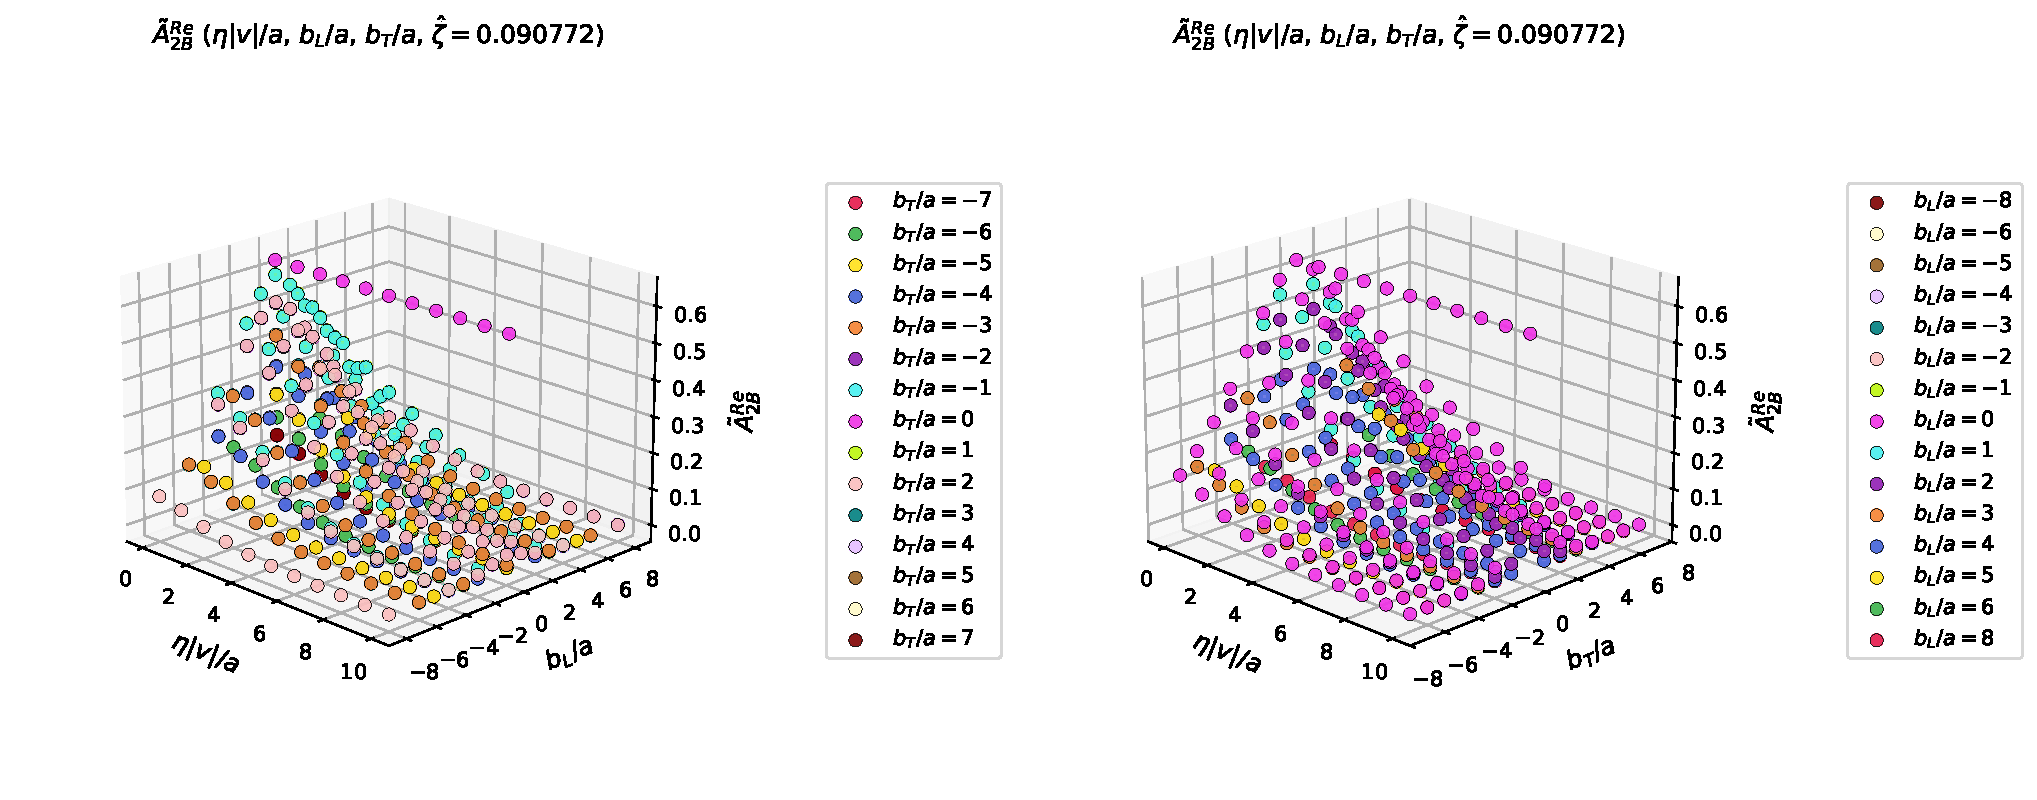
\includegraphics[width=0.98\linewidth,height=0.73\textheight,keepaspectratio]{ReA2B_PL-1_3D.pdf}\\[1mm]
{\small $\zetahat=0.090772$; $(b_L,b_T)$; staple-length dependence}
\figsrc{Thesis, Ch. 5: raw amplitude profiles; complete original panels.}
\end{frame}

\begin{frame}{$\tAmp_{2B}^{\mathrm{Re}}$ at $P_L=-1$: invariant coordinates}
\centering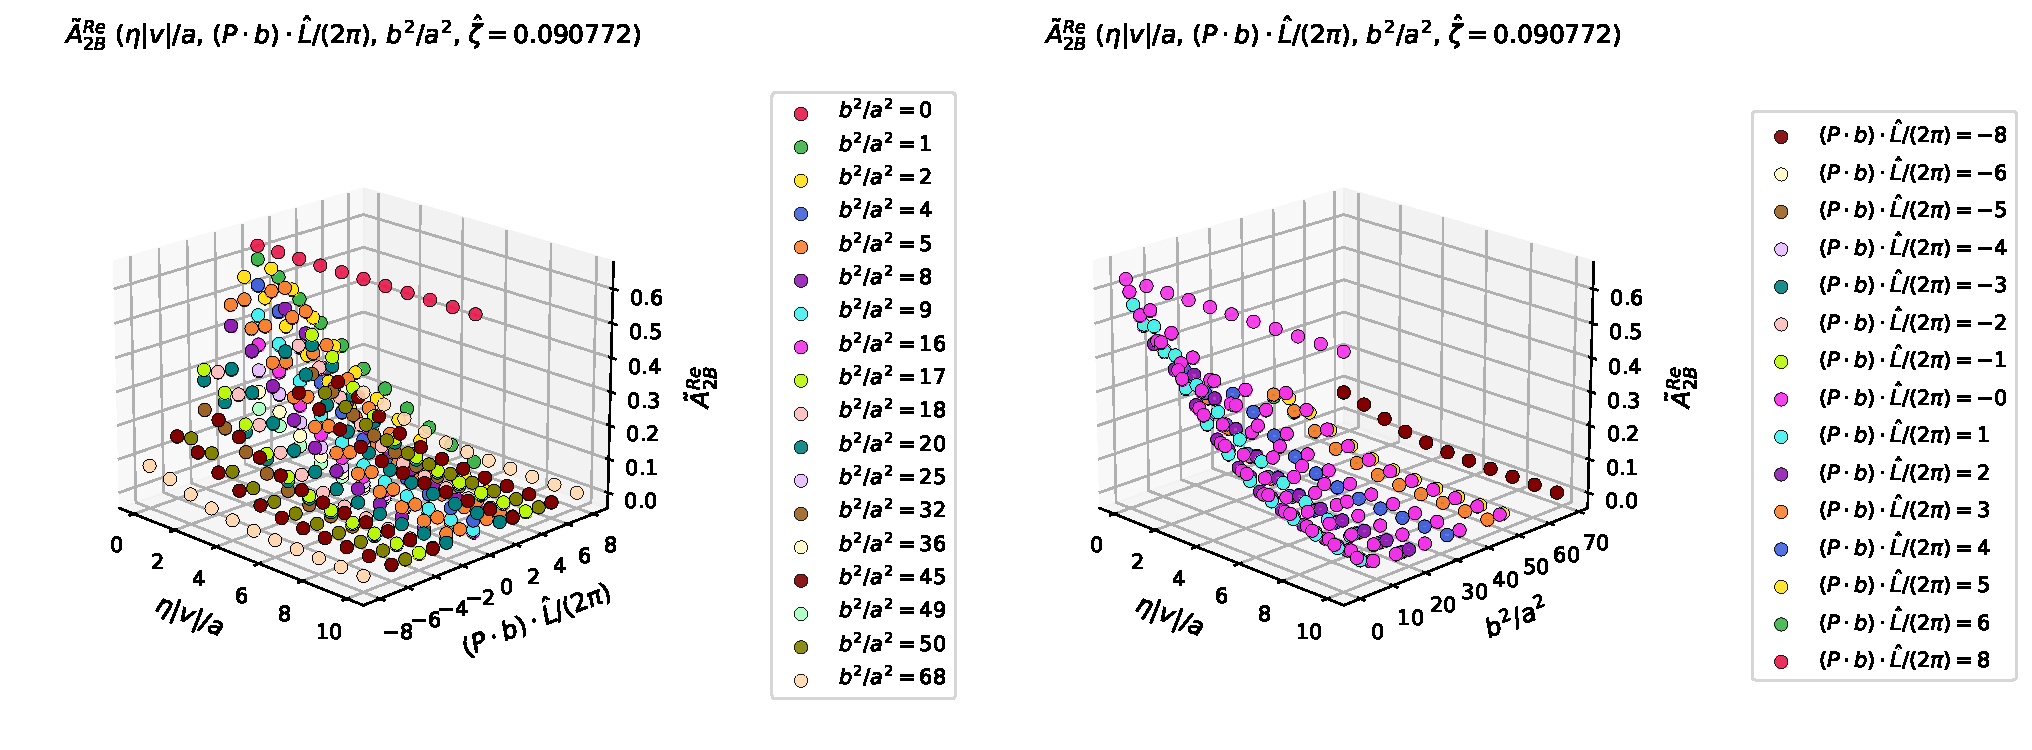
\includegraphics[width=0.98\linewidth,height=0.73\textheight,keepaspectratio]{ReA2B_Pb_bsq_PL-1_3D.pdf}\\[1mm]
{\small $\zetahat=0.090772$; $(\nu,s)$; staple-length dependence}
\figsrc{Thesis, Ch. 5: raw amplitude profiles; complete original panels.}
\end{frame}

\begin{frame}{$\tAmp_{2B}^{\mathrm{Im}}$ at $P_L=-1$: lattice coordinates}
\centering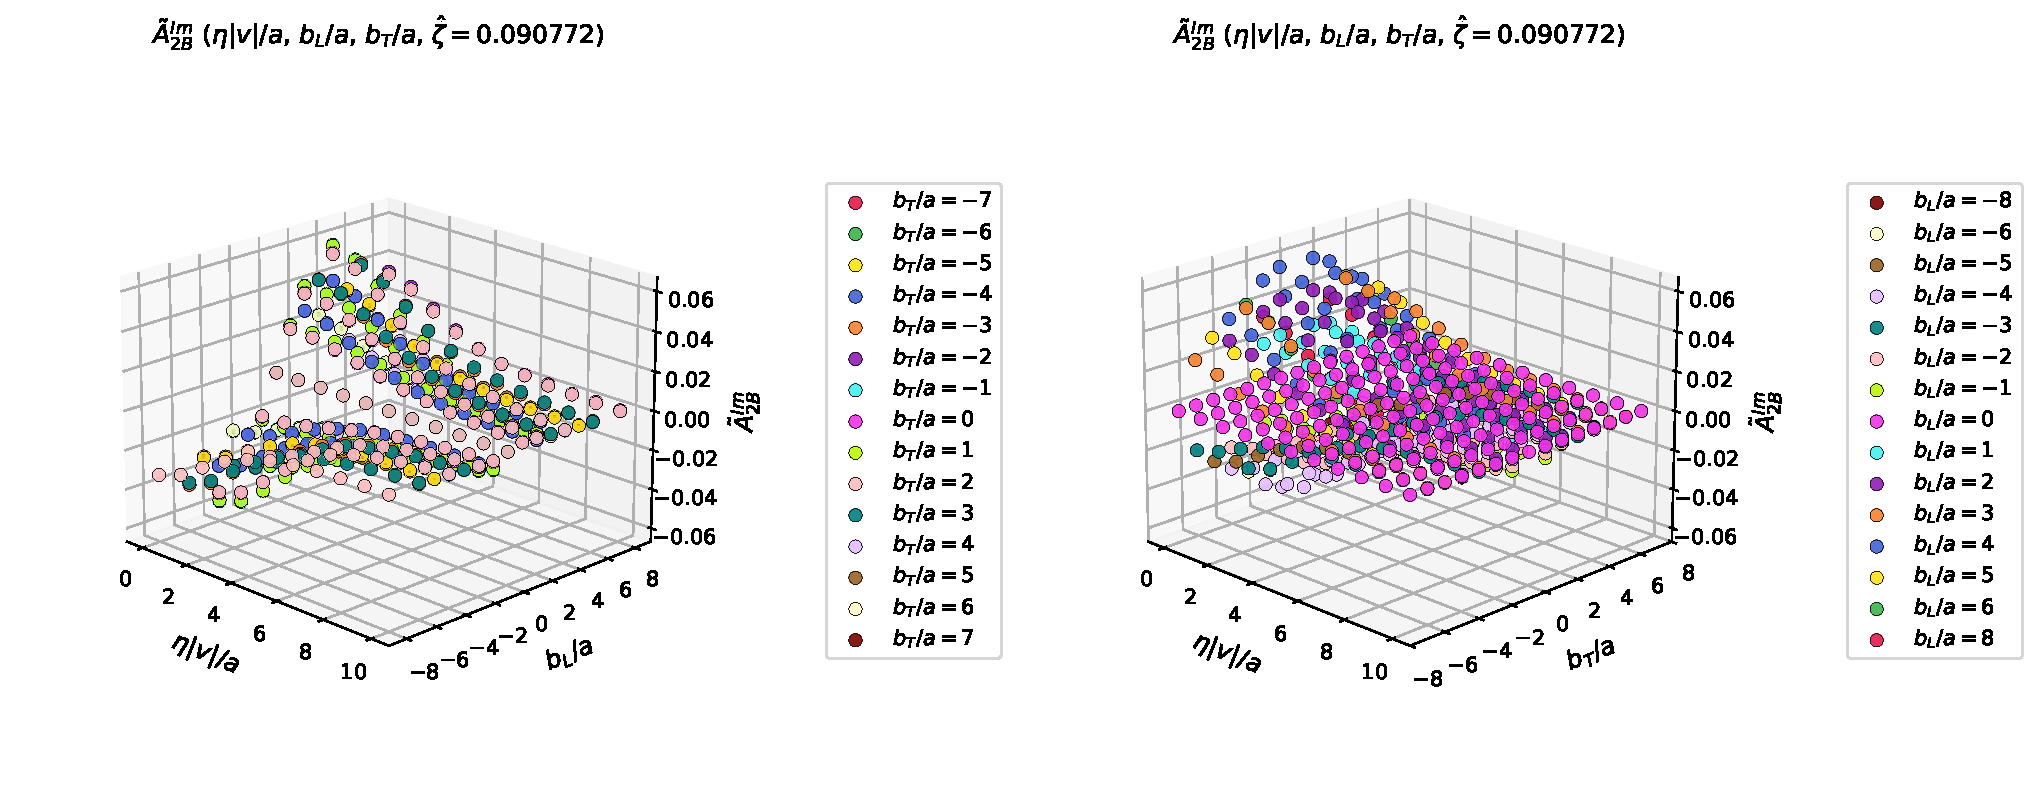
\includegraphics[width=0.98\linewidth,height=0.73\textheight,keepaspectratio]{ImA2B_PL-1_3D.pdf}\\[1mm]
{\small $\zetahat=0.090772$; $(b_L,b_T)$; staple-length dependence}
\figsrc{Thesis, Ch. 5: raw amplitude profiles; complete original panels.}
\end{frame}

\begin{frame}{$\tAmp_{2B}^{\mathrm{Im}}$ at $P_L=-1$: invariant coordinates}
\centering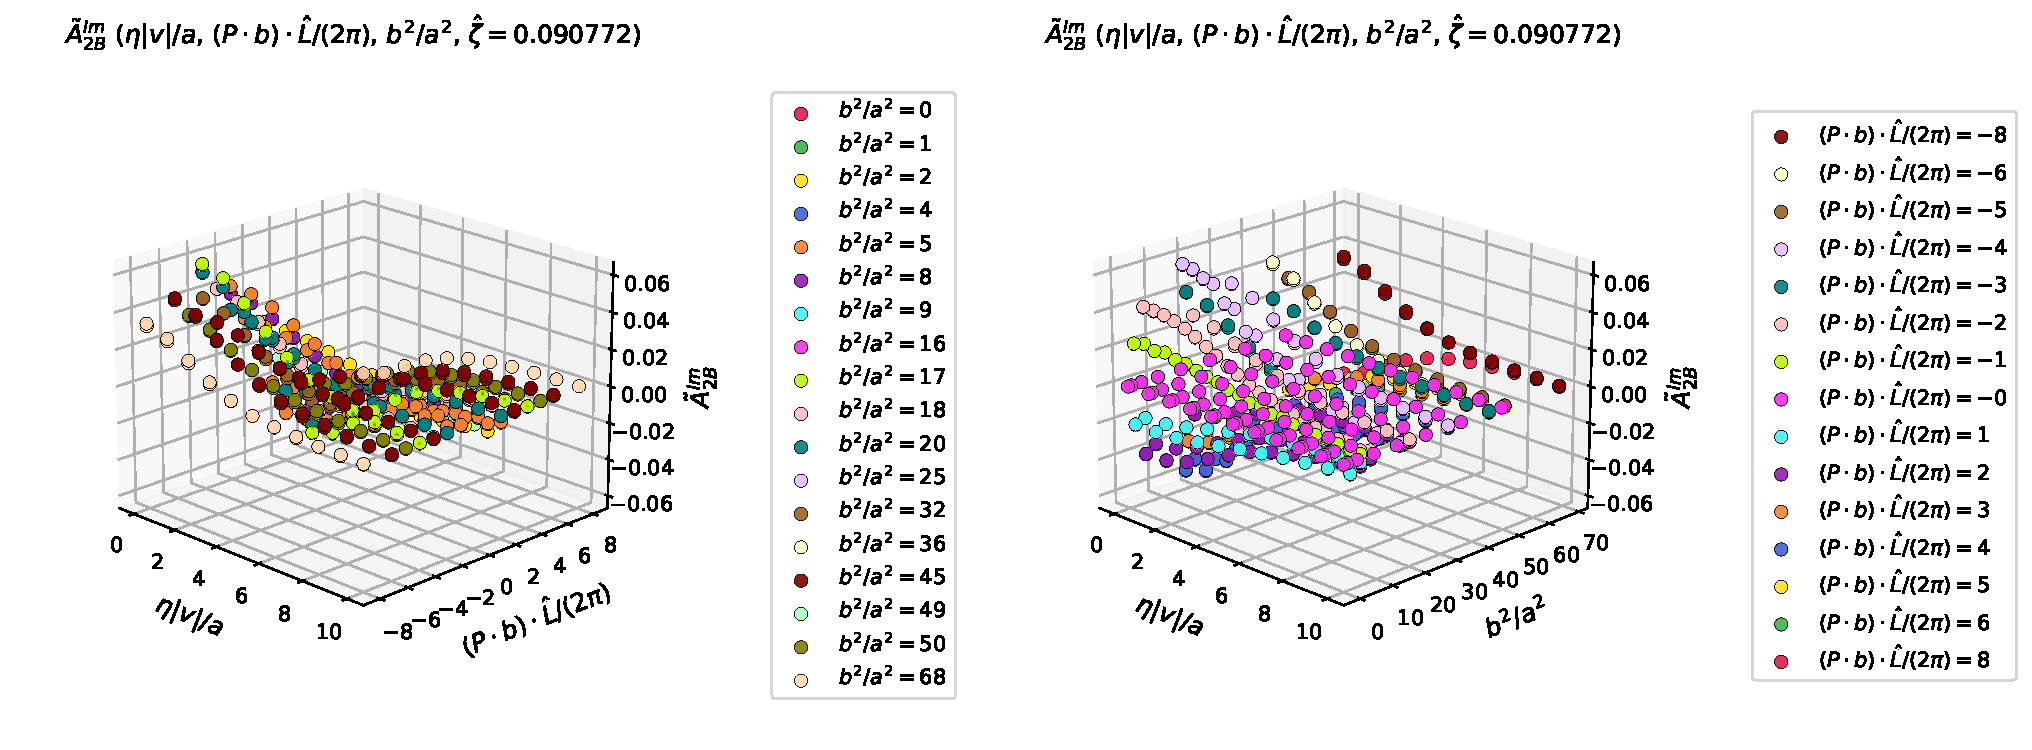
\includegraphics[width=0.98\linewidth,height=0.73\textheight,keepaspectratio]{ImA2B_Pb_bsq_PL-1_3D.pdf}\\[1mm]
{\small $\zetahat=0.090772$; $(\nu,s)$; staple-length dependence}
\figsrc{Thesis, Ch. 5: raw amplitude profiles; complete original panels.}
\end{frame}

\begin{frame}{$\tAmp_{12B}^{\mathrm{Re}}$ at $P_L=-1$: lattice coordinates}
\centering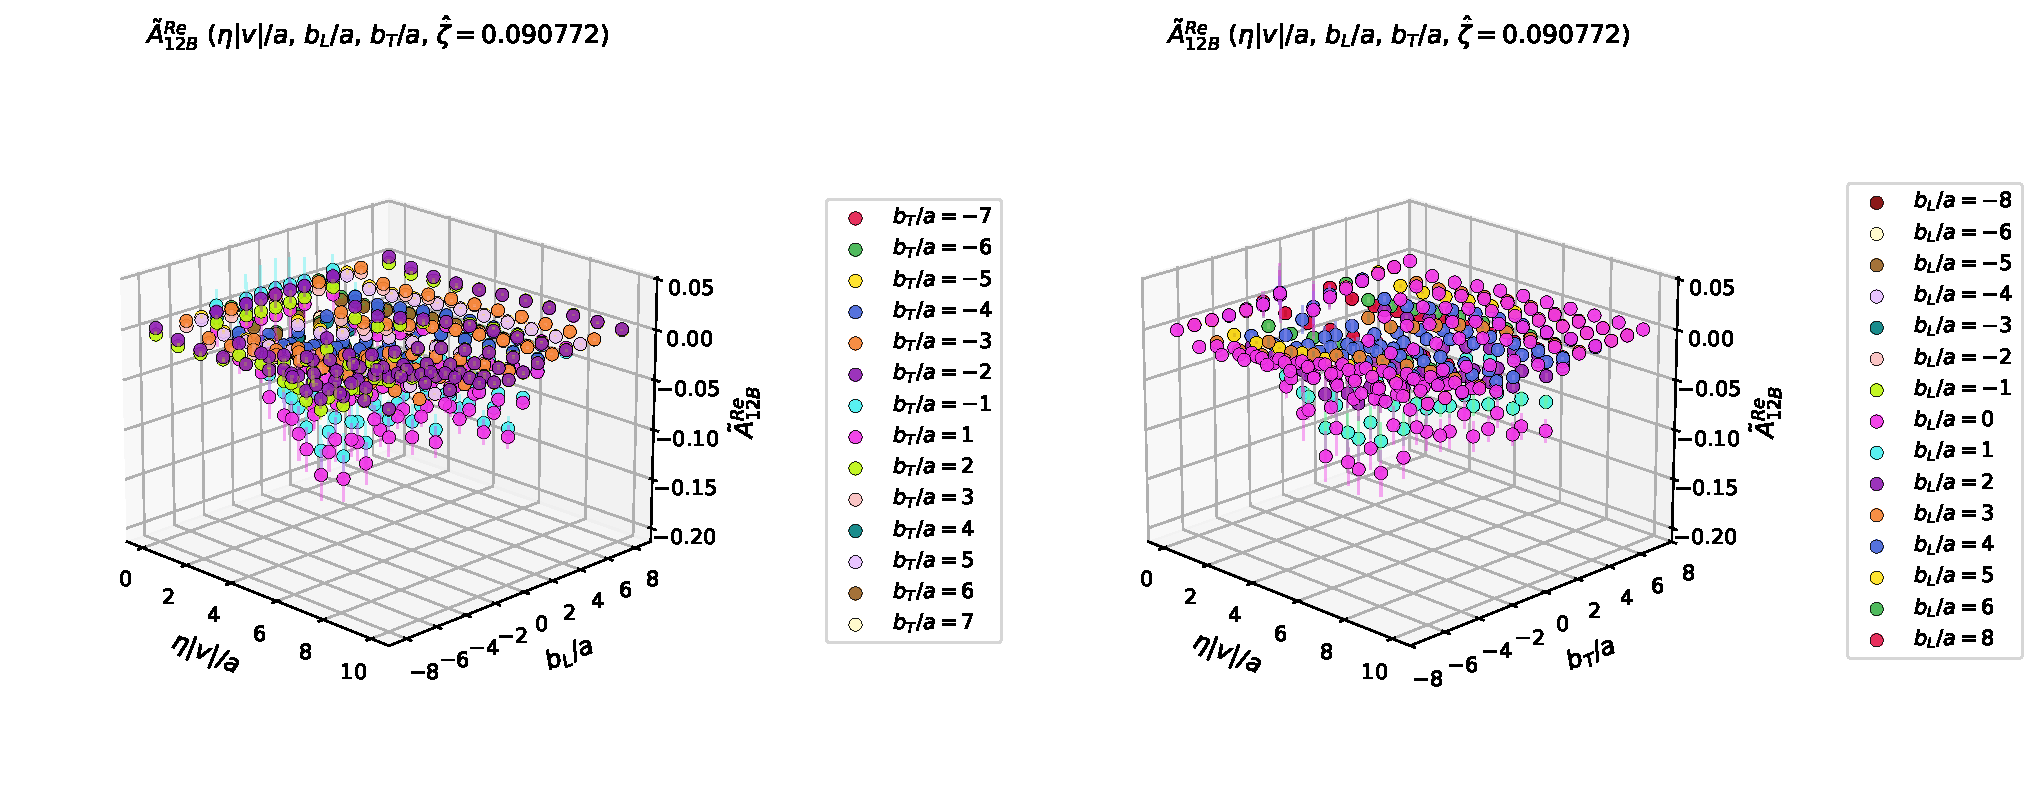
\includegraphics[width=0.98\linewidth,height=0.73\textheight,keepaspectratio]{ReA12B_PL-1_3D.pdf}\\[1mm]
{\small $\zetahat=0.090772$; $(b_L,b_T)$; staple-length dependence}
\figsrc{Thesis, Ch. 5: raw amplitude profiles; complete original panels.}
\end{frame}

\begin{frame}{$\tAmp_{12B}^{\mathrm{Re}}$ at $P_L=-1$: invariant coordinates}
\centering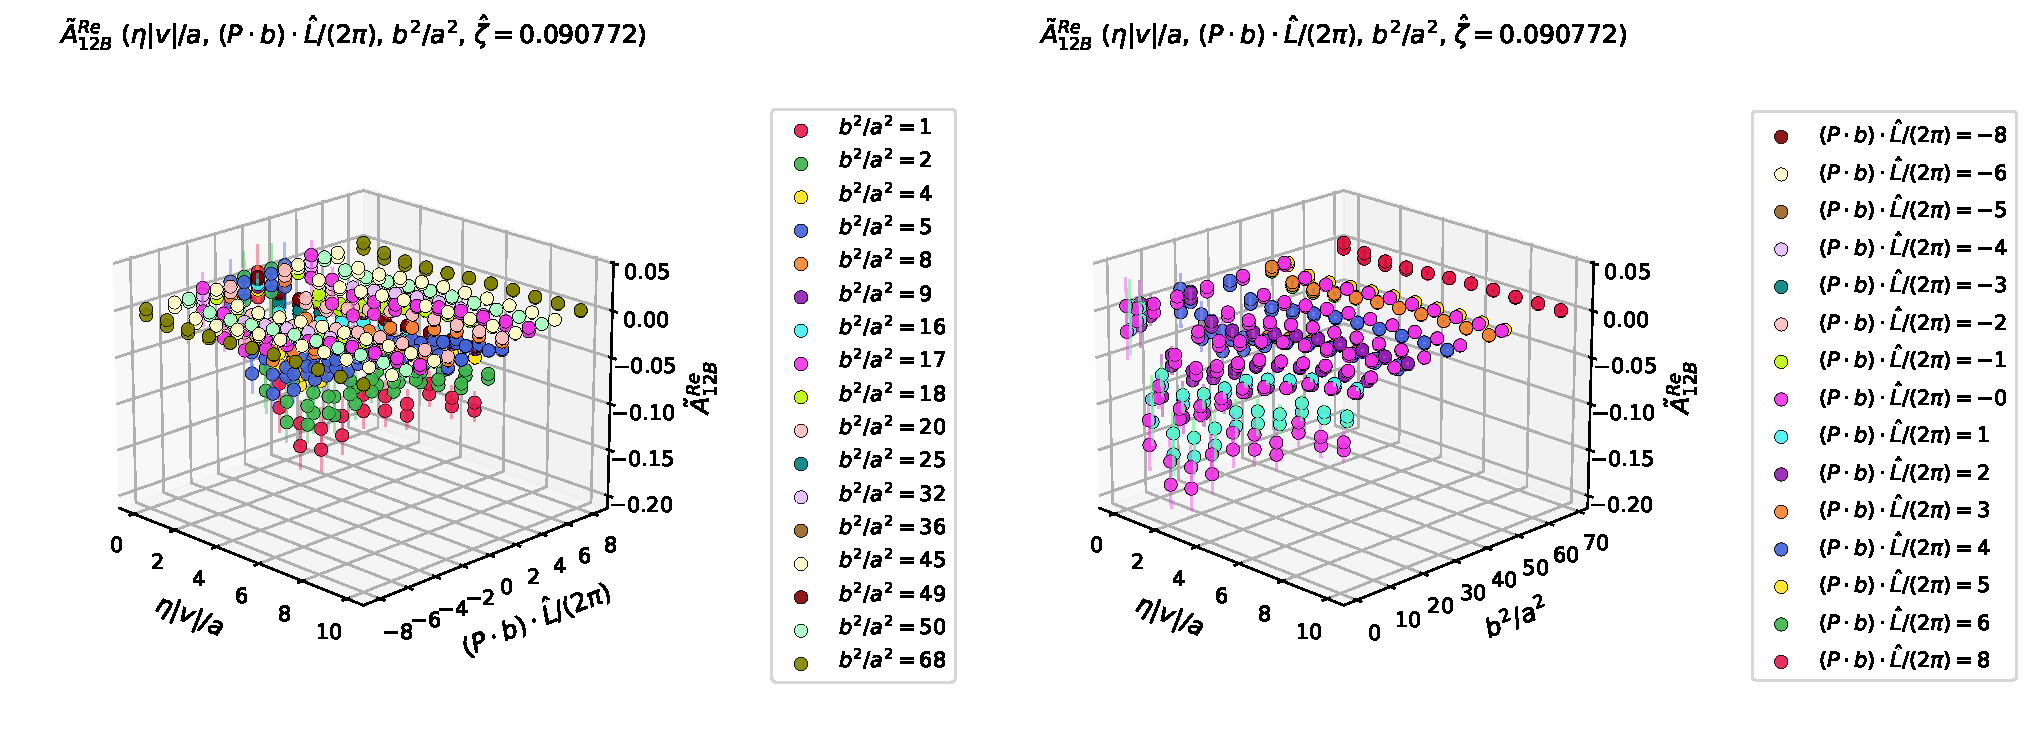
\includegraphics[width=0.98\linewidth,height=0.73\textheight,keepaspectratio]{ReA12B_Pb_bsq_PL-1_3D.pdf}\\[1mm]
{\small $\zetahat=0.090772$; $(\nu,s)$; staple-length dependence}
\figsrc{Thesis, Ch. 5: raw amplitude profiles; complete original panels.}
\end{frame}

\begin{frame}{$\tAmp_{12B}^{\mathrm{Im}}$ at $P_L=-1$: lattice coordinates}
\centering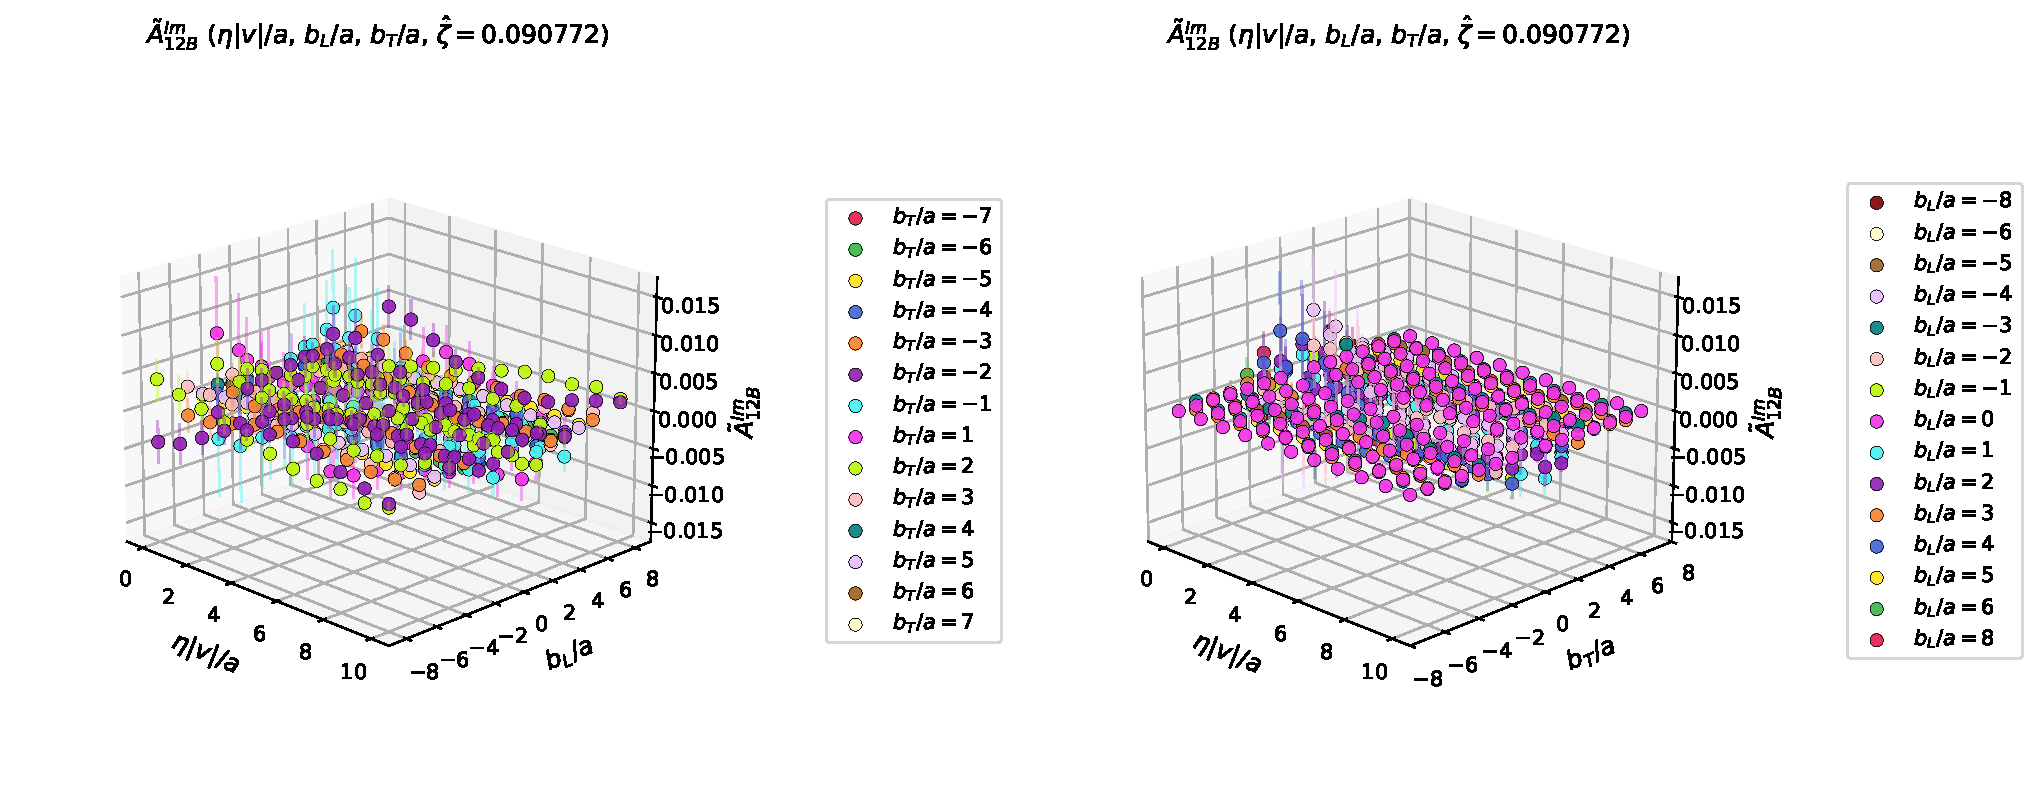
\includegraphics[width=0.98\linewidth,height=0.73\textheight,keepaspectratio]{ImA12B_PL-1_3D.pdf}\\[1mm]
{\small $\zetahat=0.090772$; $(b_L,b_T)$; staple-length dependence}
\figsrc{Thesis, Ch. 5: raw amplitude profiles; complete original panels.}
\end{frame}

\begin{frame}{$\tAmp_{12B}^{\mathrm{Im}}$ at $P_L=-1$: invariant coordinates}
\centering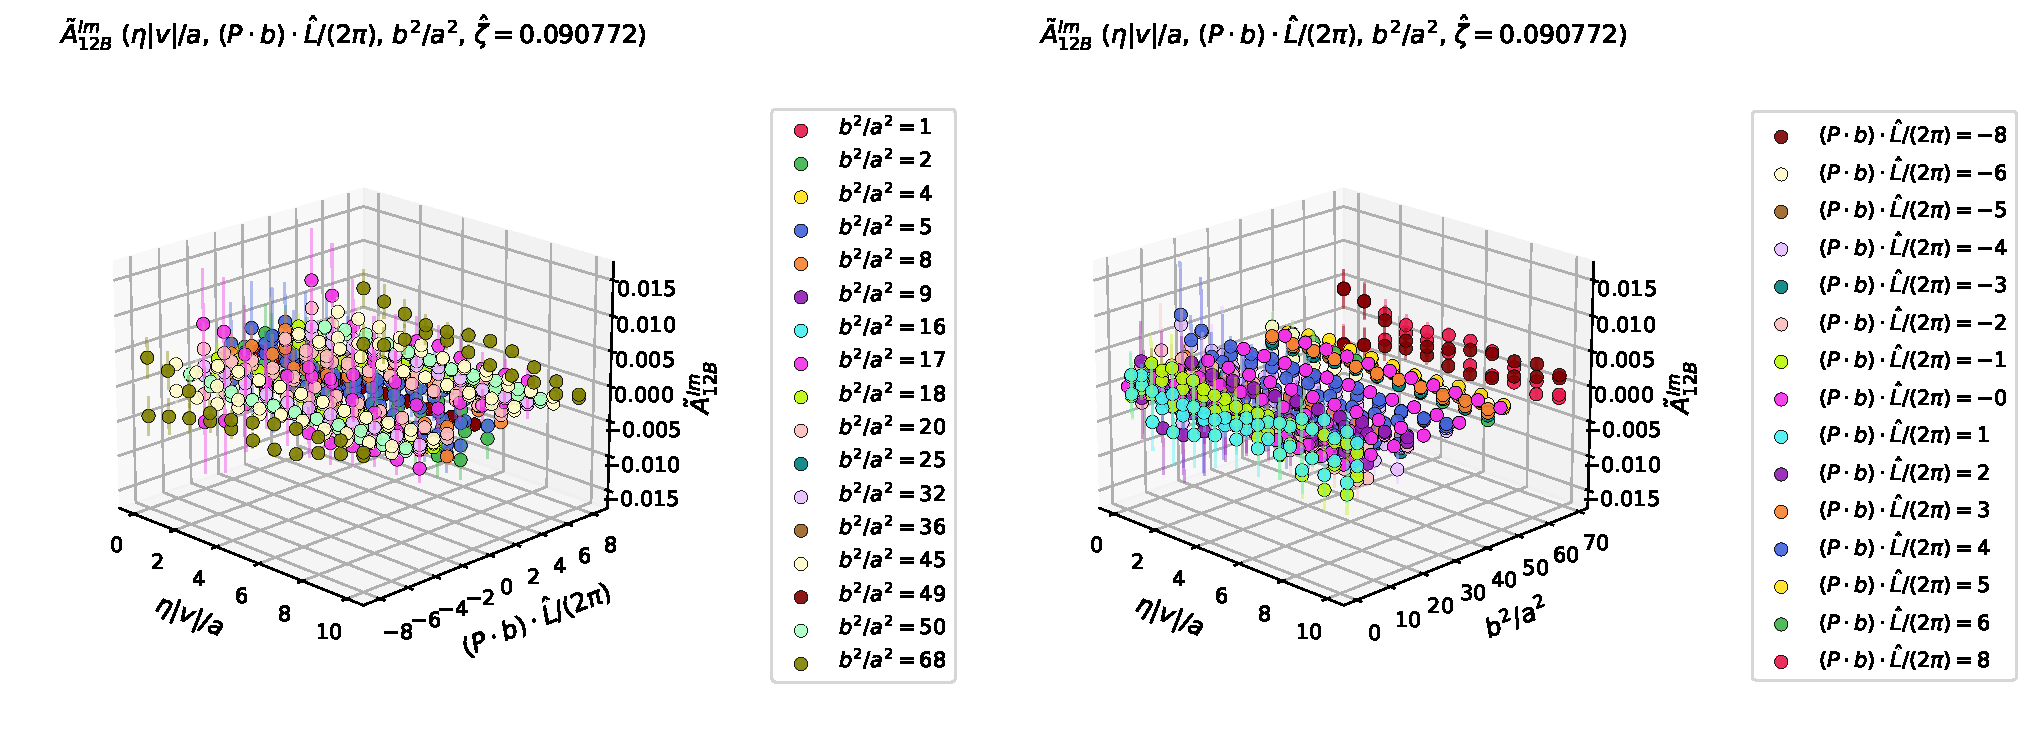
\includegraphics[width=0.98\linewidth,height=0.73\textheight,keepaspectratio]{ImA12B_Pb_bsq_PL-1_3D.pdf}\\[1mm]
{\small $\zetahat=0.090772$; $(\nu,s)$; staple-length dependence}
\figsrc{Thesis, Ch. 5: raw amplitude profiles; complete original panels.}
\end{frame}

\begin{frame}{$\tAmp_{2B}^{\mathrm{Re}}$ at $P_L=-1$: lattice coordinates}
\centering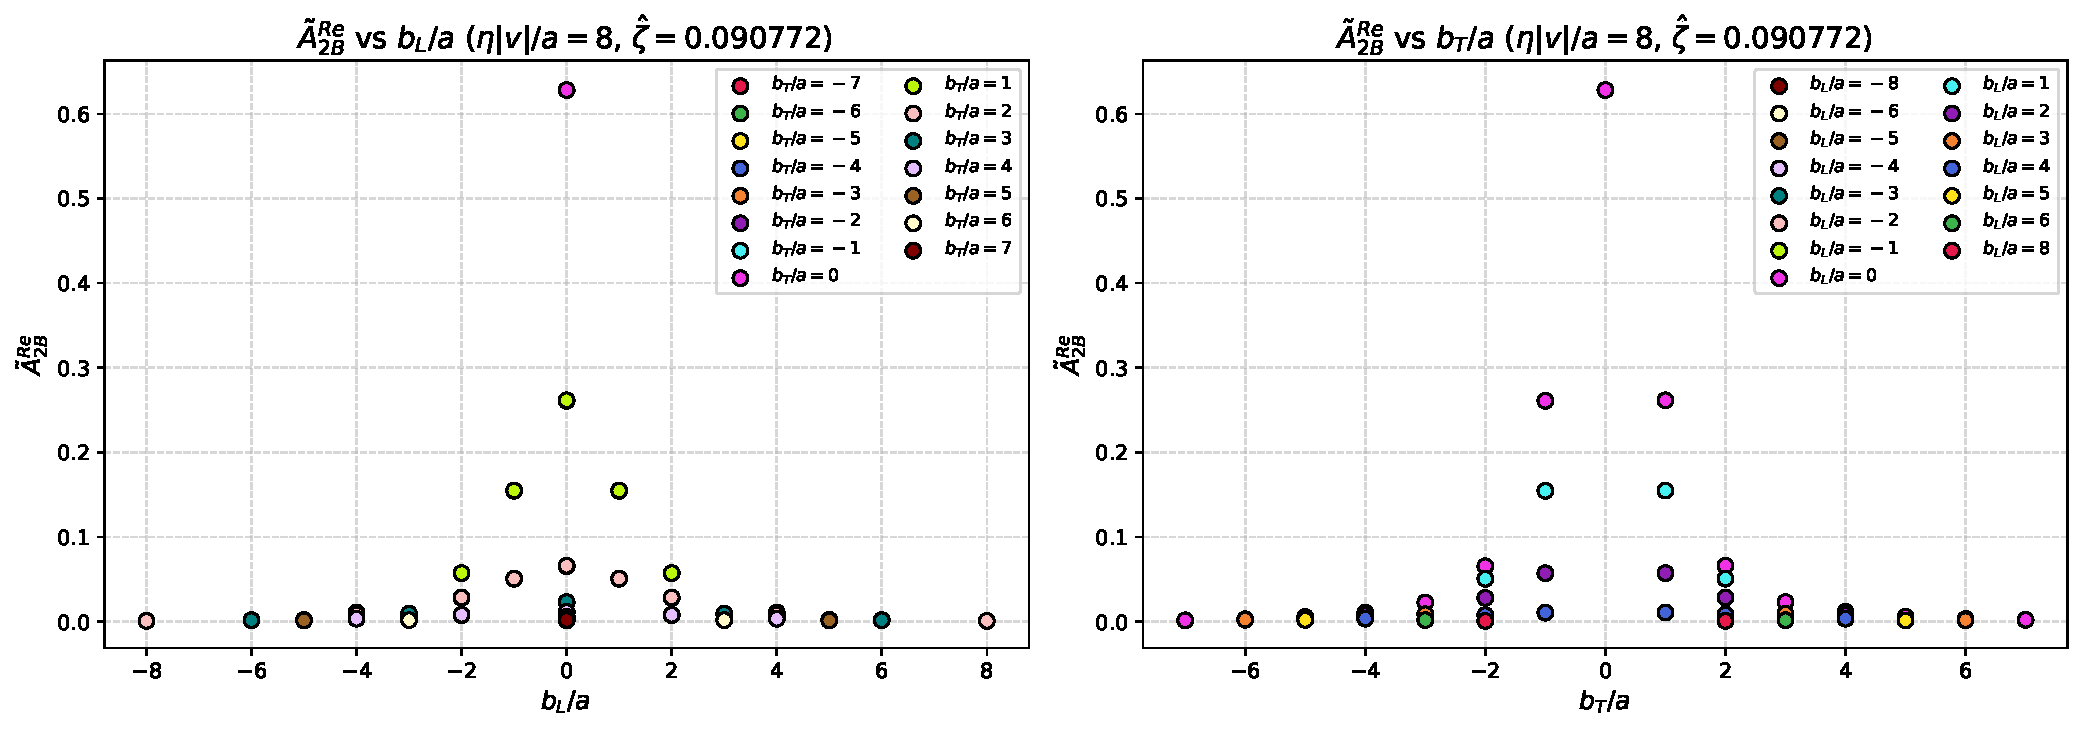
\includegraphics[width=0.98\linewidth,height=0.73\textheight,keepaspectratio]{ReA2B_eta8_PL-1_2D.pdf}\\[1mm]
{\small $\zetahat=0.090772$; $(b_L,b_T)$; $\eta|v|/a=8$ slices}
\figsrc{Thesis, Ch. 5: raw amplitude profiles; complete original panels.}
\end{frame}

\begin{frame}{$\tAmp_{2B}^{\mathrm{Re}}$ at $P_L=-1$: invariant coordinates}
\centering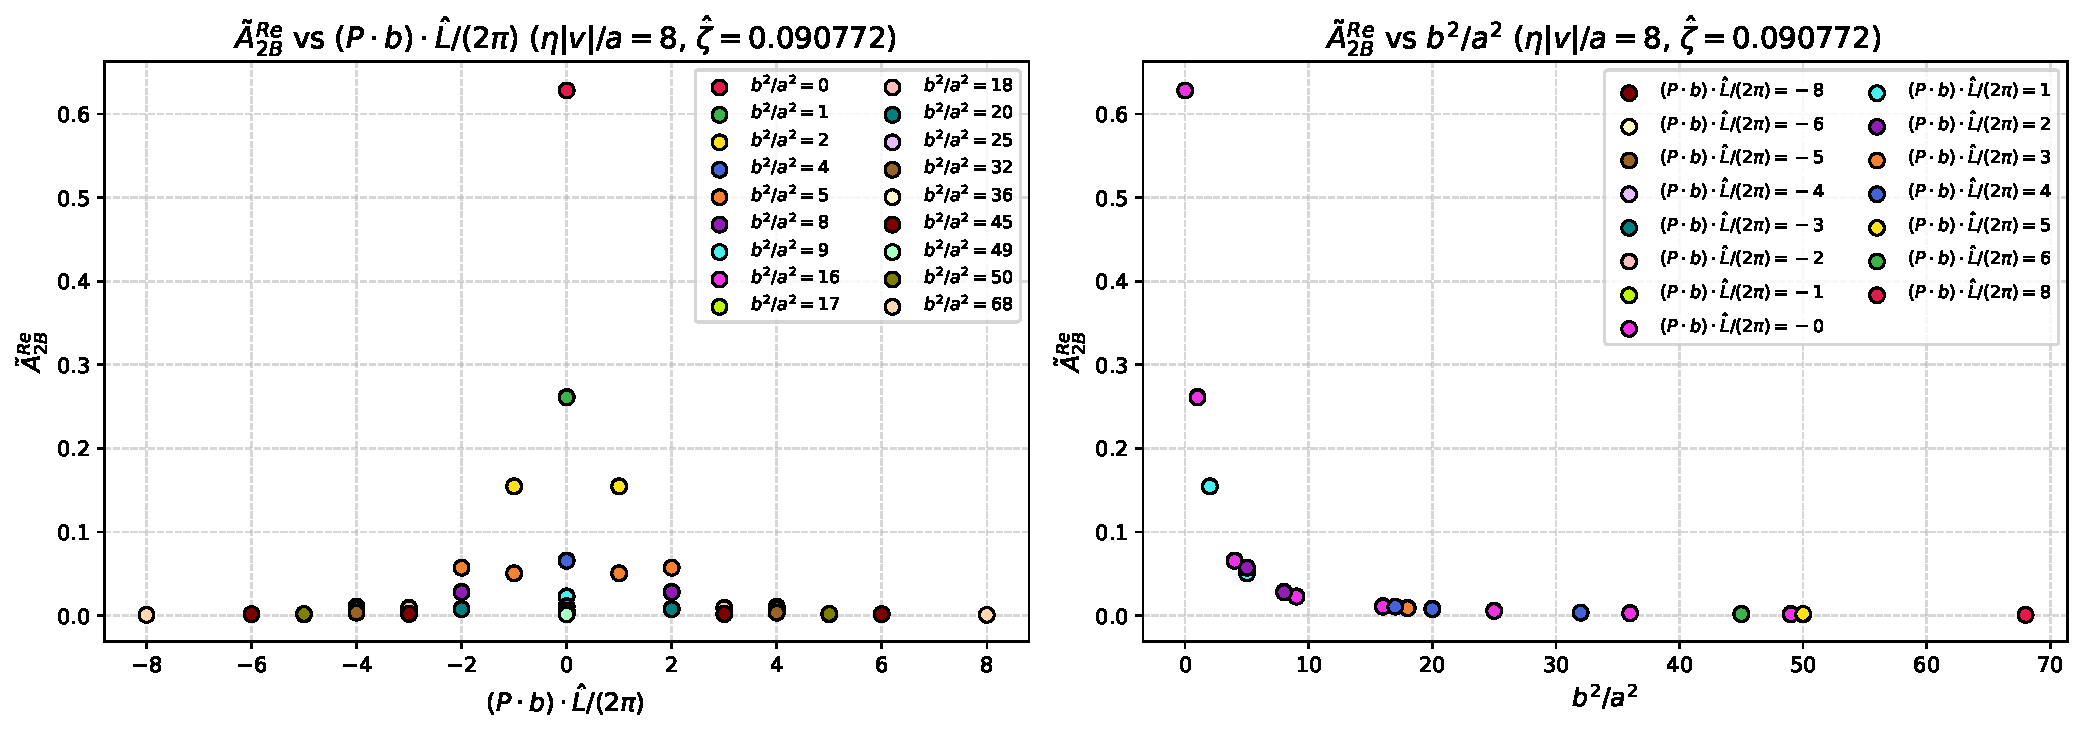
\includegraphics[width=0.98\linewidth,height=0.73\textheight,keepaspectratio]{ReA2B_Pb_bsq_eta8_PL-1_2D.pdf}\\[1mm]
{\small $\zetahat=0.090772$; $(\nu,s)$; $\eta|v|/a=8$ slices}
\figsrc{Thesis, Ch. 5: raw amplitude profiles; complete original panels.}
\end{frame}

\begin{frame}{$\tAmp_{2B}^{\mathrm{Im}}$ at $P_L=-1$: lattice coordinates}
\centering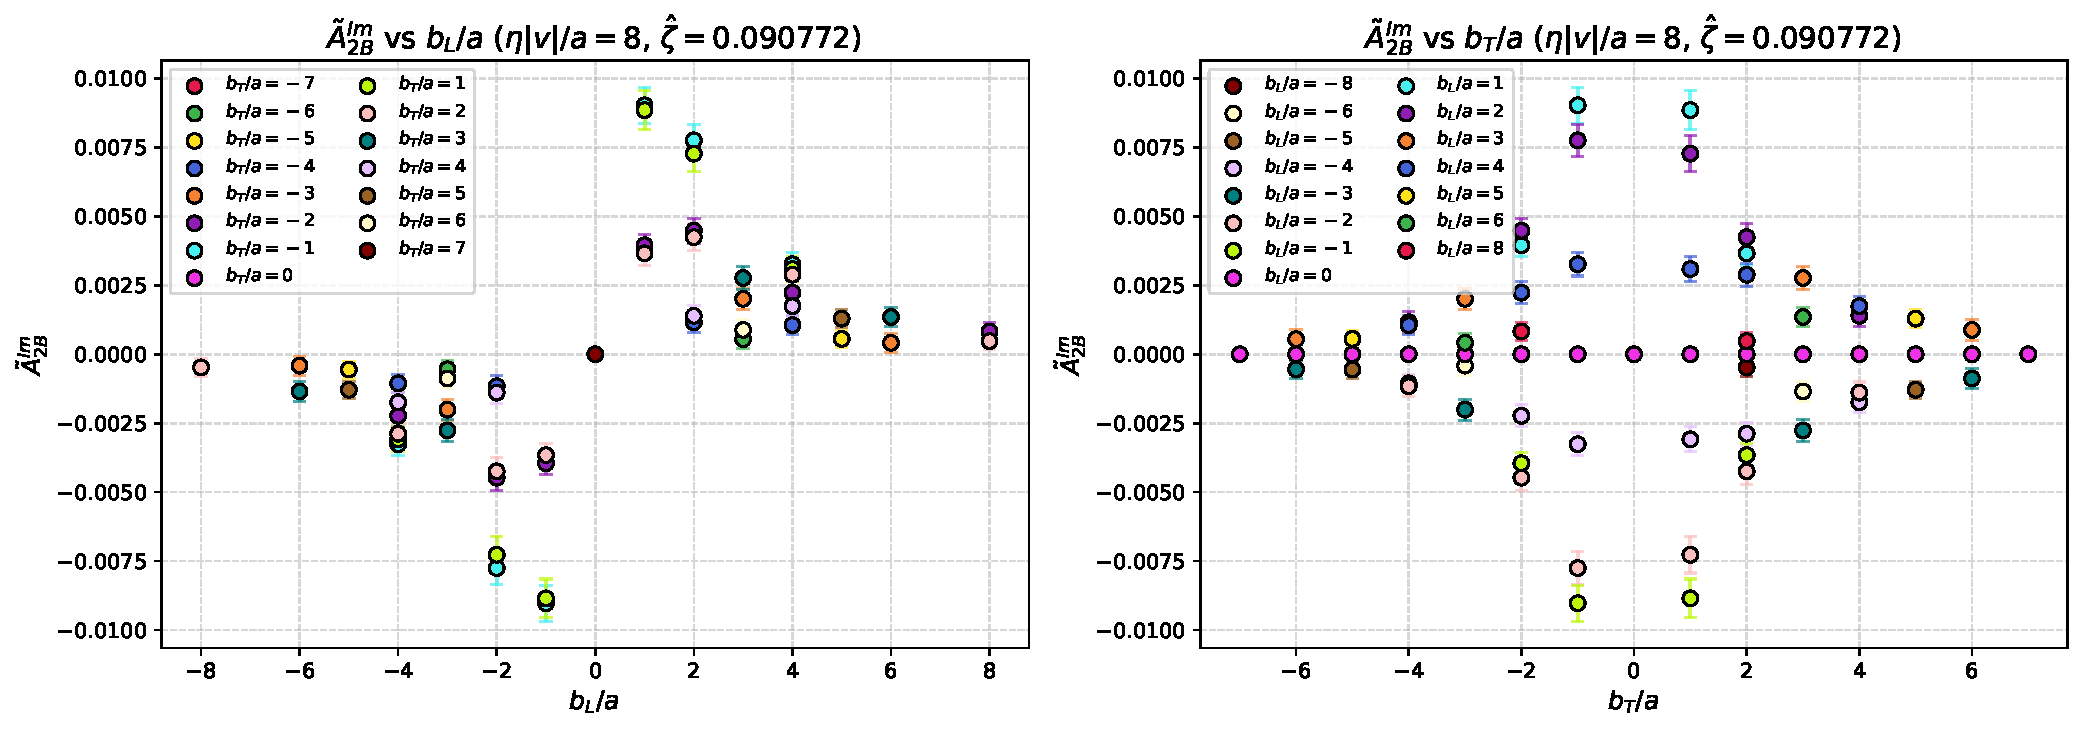
\includegraphics[width=0.98\linewidth,height=0.73\textheight,keepaspectratio]{ImA2B_eta8_PL-1_2D.pdf}\\[1mm]
{\small $\zetahat=0.090772$; $(b_L,b_T)$; $\eta|v|/a=8$ slices}
\figsrc{Thesis, Ch. 5: raw amplitude profiles; complete original panels.}
\end{frame}

\begin{frame}{$\tAmp_{2B}^{\mathrm{Im}}$ at $P_L=-1$: invariant coordinates}
\centering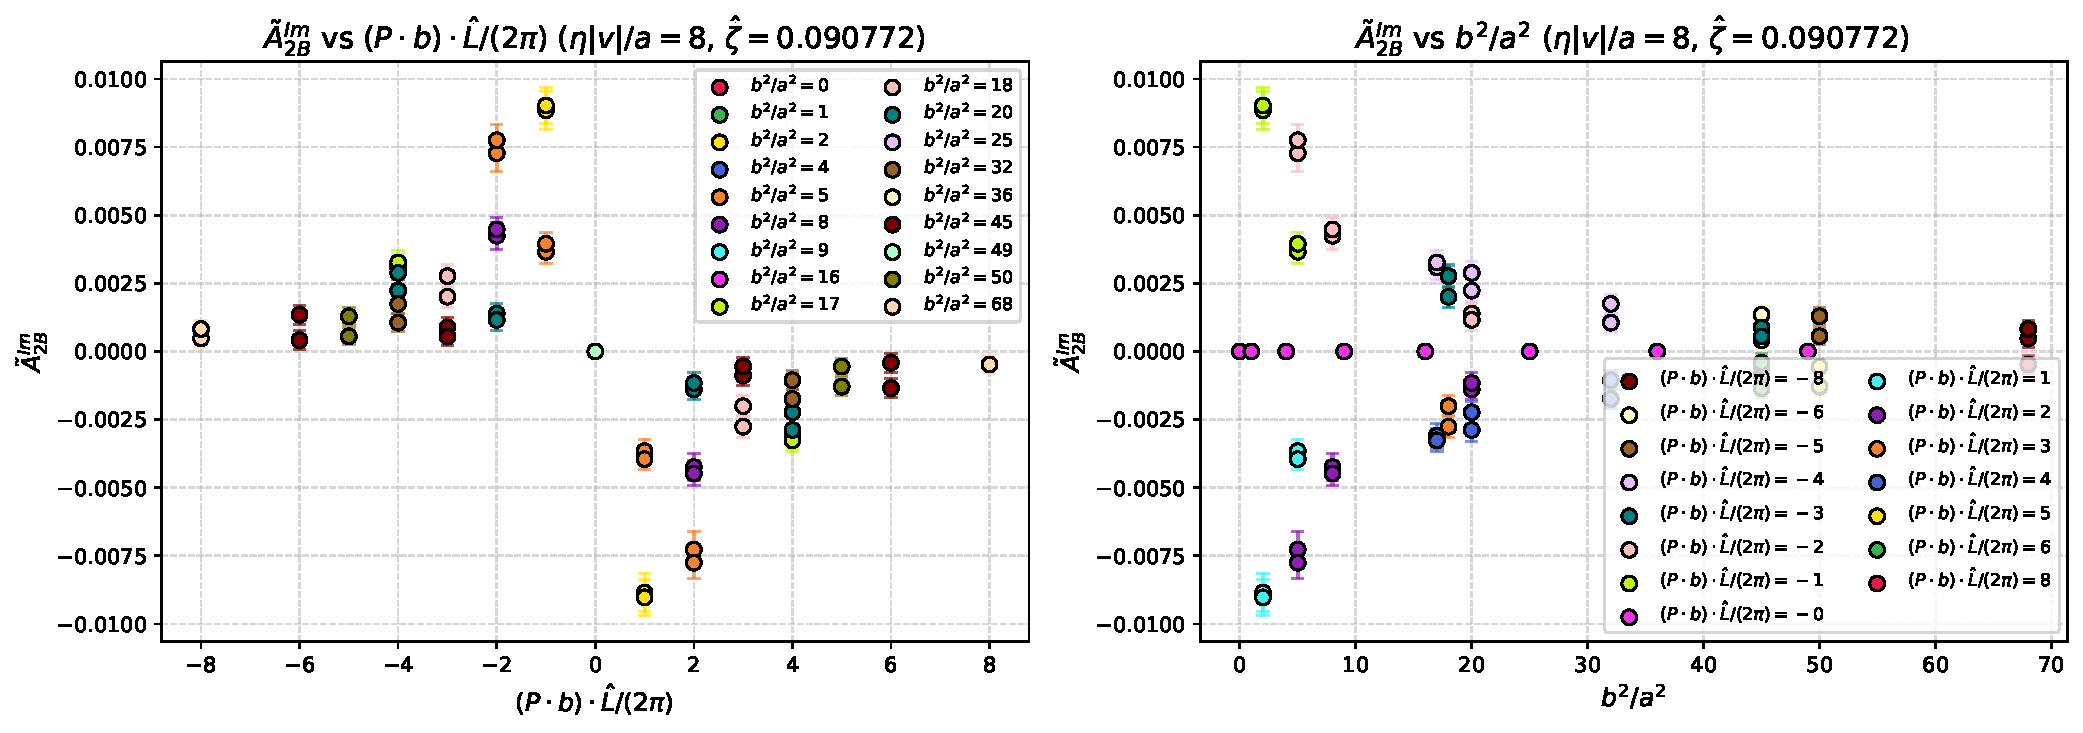
\includegraphics[width=0.98\linewidth,height=0.73\textheight,keepaspectratio]{ImA2B_Pb_bsq_eta8_PL-1_2D.pdf}\\[1mm]
{\small $\zetahat=0.090772$; $(\nu,s)$; $\eta|v|/a=8$ slices}
\figsrc{Thesis, Ch. 5: raw amplitude profiles; complete original panels.}
\end{frame}

\begin{frame}{$\tAmp_{12B}^{\mathrm{Re}}$ at $P_L=-1$: lattice coordinates}
\centering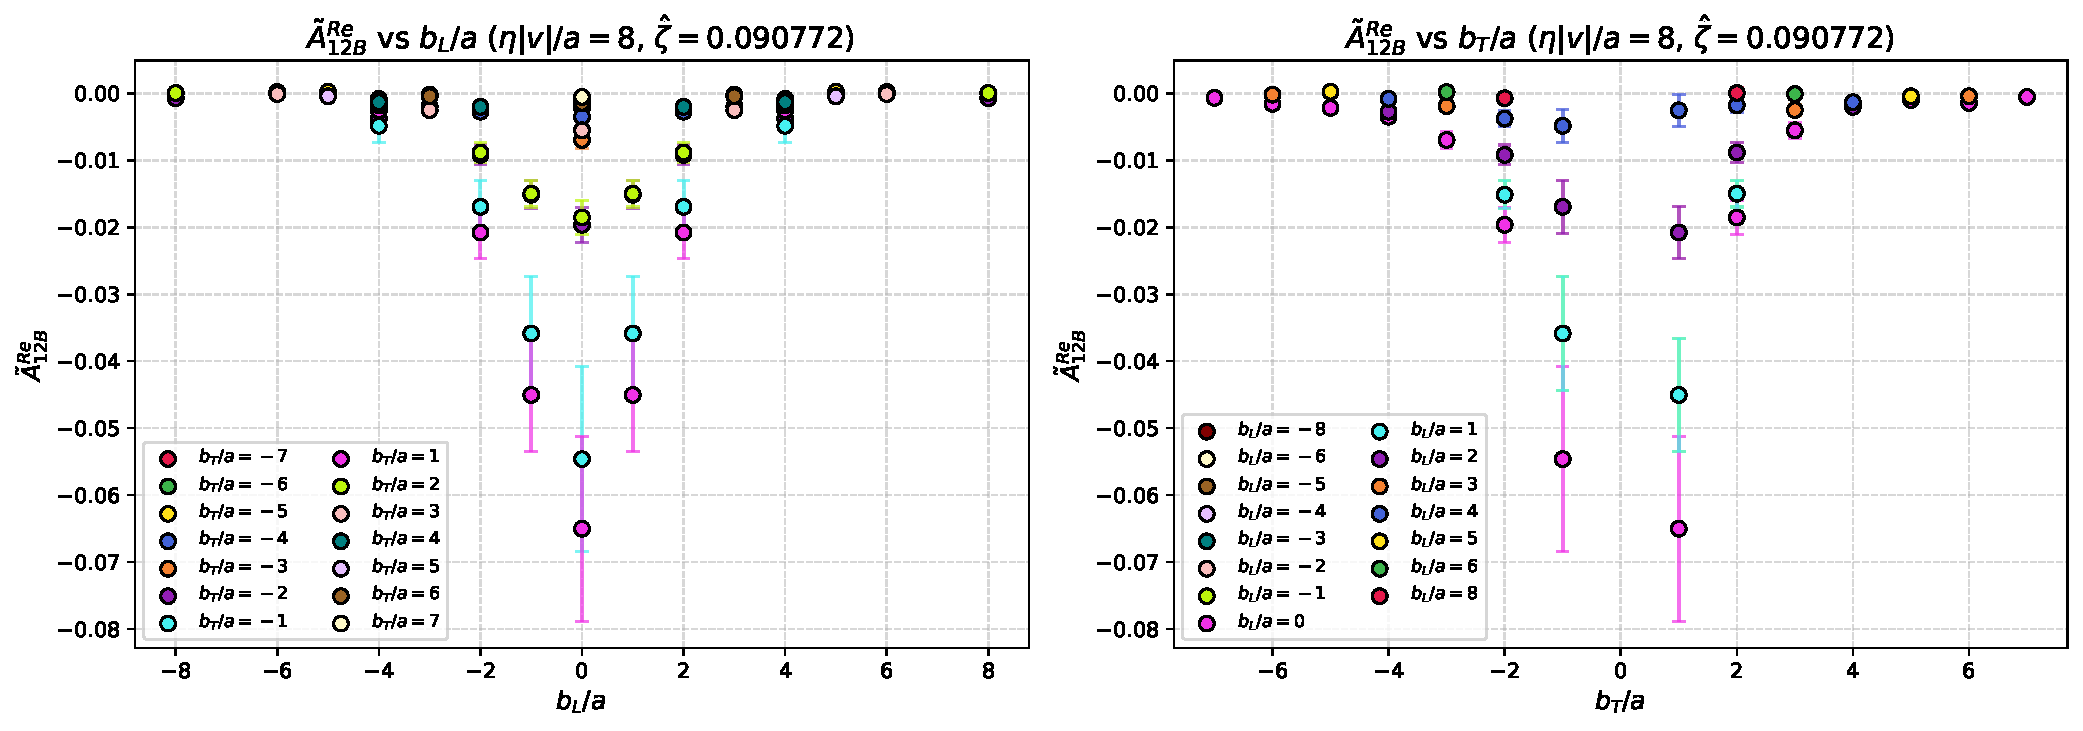
\includegraphics[width=0.98\linewidth,height=0.73\textheight,keepaspectratio]{ReA12B_eta8_PL-1_2D.pdf}\\[1mm]
{\small $\zetahat=0.090772$; $(b_L,b_T)$; $\eta|v|/a=8$ slices}
\figsrc{Thesis, Ch. 5: raw amplitude profiles; complete original panels.}
\end{frame}

\begin{frame}{$\tAmp_{12B}^{\mathrm{Re}}$ at $P_L=-1$: invariant coordinates}
\centering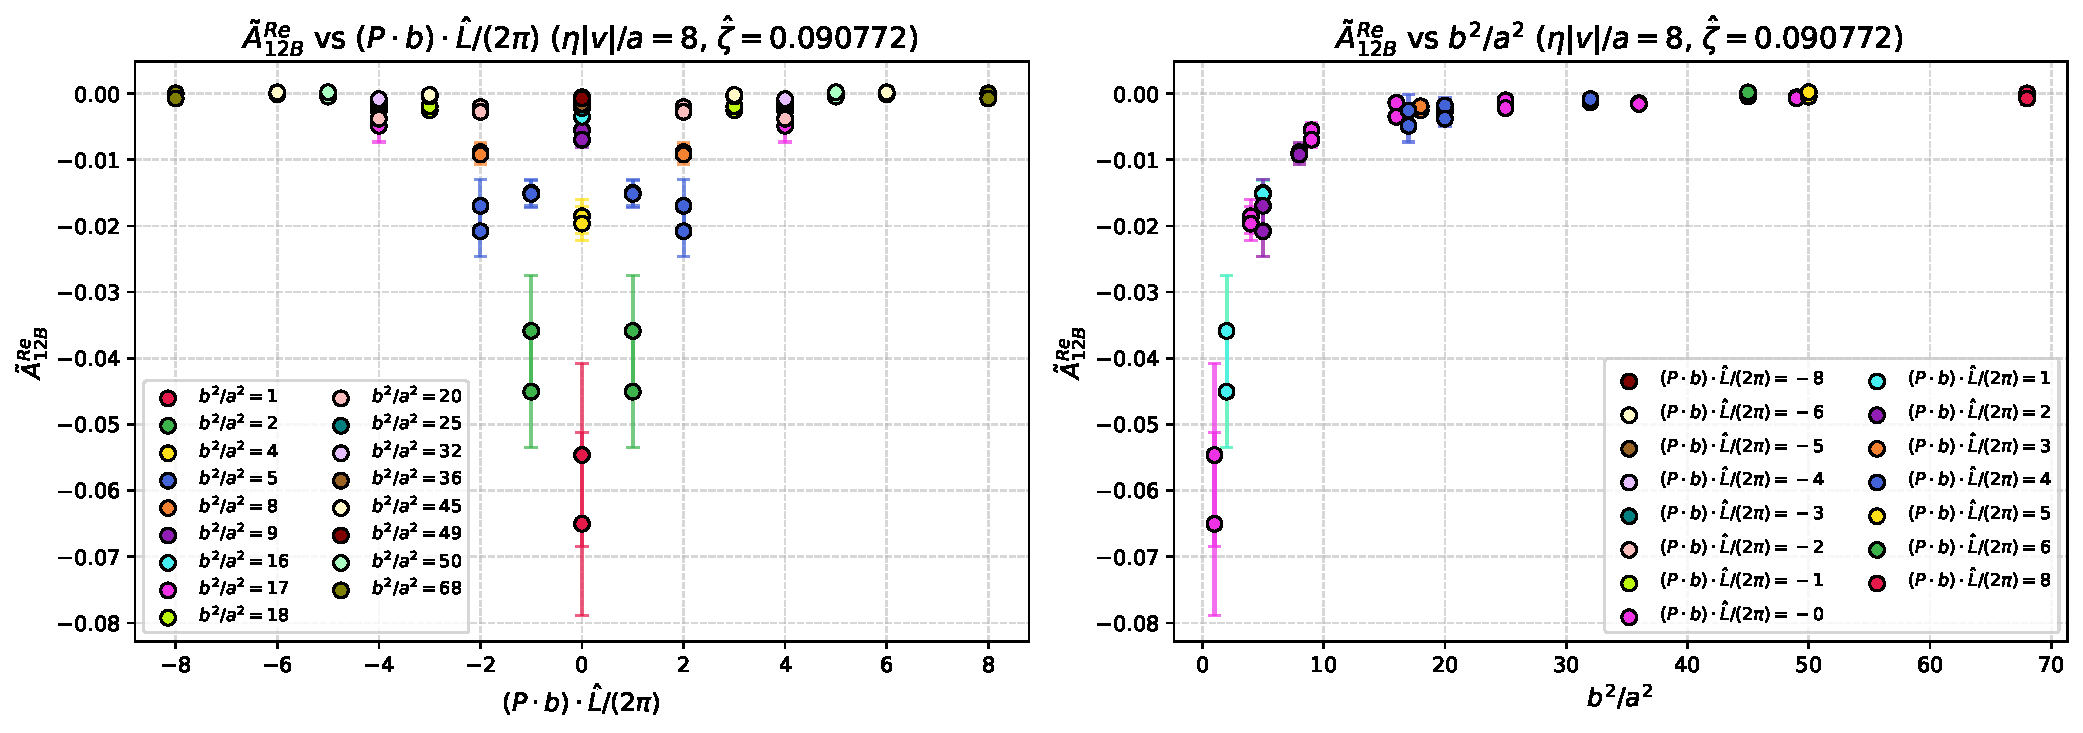
\includegraphics[width=0.98\linewidth,height=0.73\textheight,keepaspectratio]{ReA12B_Pb_bsq_eta8_PL-1_2D.pdf}\\[1mm]
{\small $\zetahat=0.090772$; $(\nu,s)$; $\eta|v|/a=8$ slices}
\figsrc{Thesis, Ch. 5: raw amplitude profiles; complete original panels.}
\end{frame}

\begin{frame}{$\tAmp_{12B}^{\mathrm{Im}}$ at $P_L=-1$: lattice coordinates}
\centering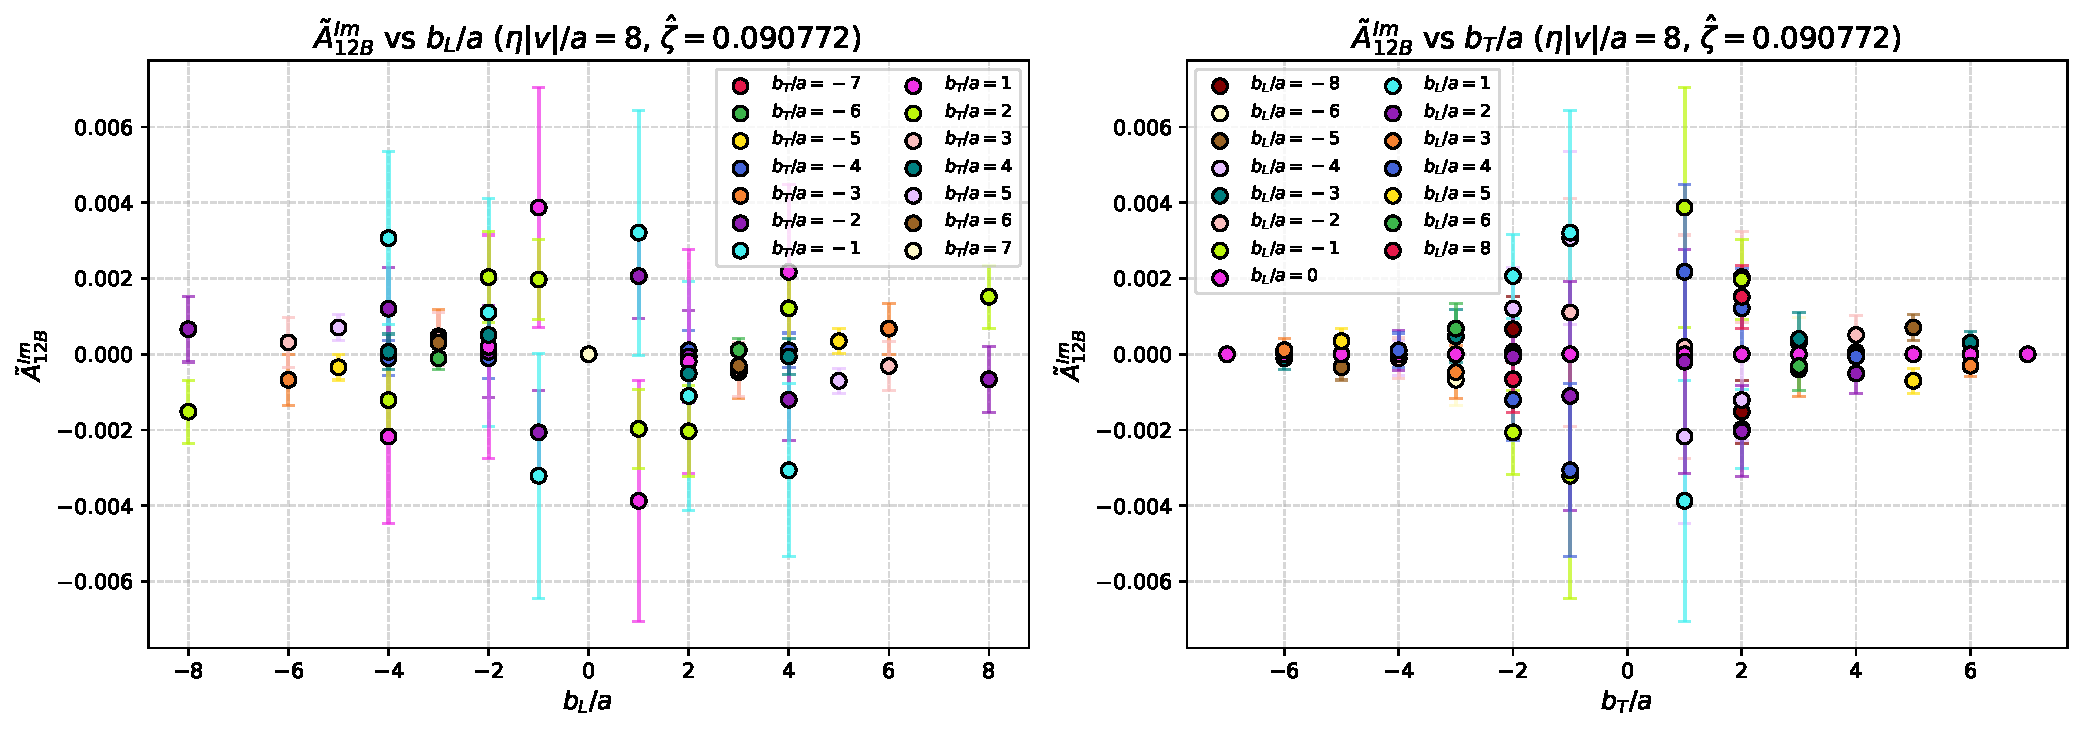
\includegraphics[width=0.98\linewidth,height=0.73\textheight,keepaspectratio]{ImA12B_eta8_PL-1_2D.pdf}\\[1mm]
{\small $\zetahat=0.090772$; $(b_L,b_T)$; $\eta|v|/a=8$ slices}
\figsrc{Thesis, Ch. 5: raw amplitude profiles; complete original panels.}
\end{frame}

\begin{frame}{$\tAmp_{12B}^{\mathrm{Im}}$ at $P_L=-1$: invariant coordinates}
\centering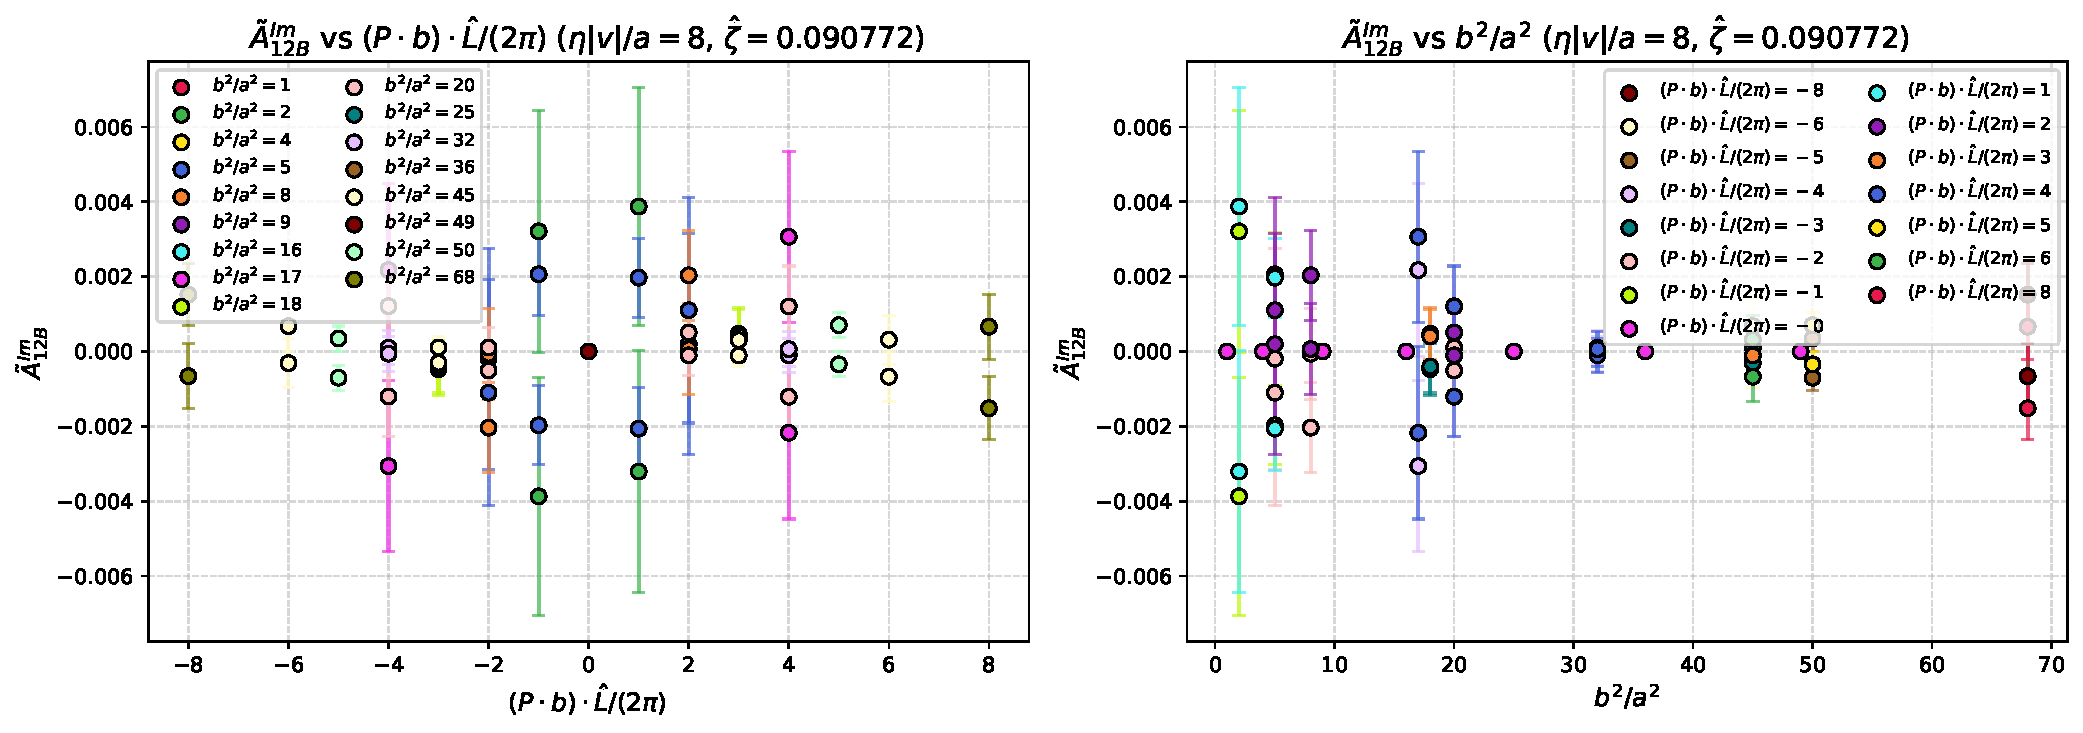
\includegraphics[width=0.98\linewidth,height=0.73\textheight,keepaspectratio]{ImA12B_Pb_bsq_eta8_PL-1_2D.pdf}\\[1mm]
{\small $\zetahat=0.090772$; $(\nu,s)$; $\eta|v|/a=8$ slices}
\figsrc{Thesis, Ch. 5: raw amplitude profiles; complete original panels.}
\end{frame}

\begin{frame}{$\tAmp_{2B}^{\mathrm{Re}}$ at $P_L=-2$: lattice coordinates}
\centering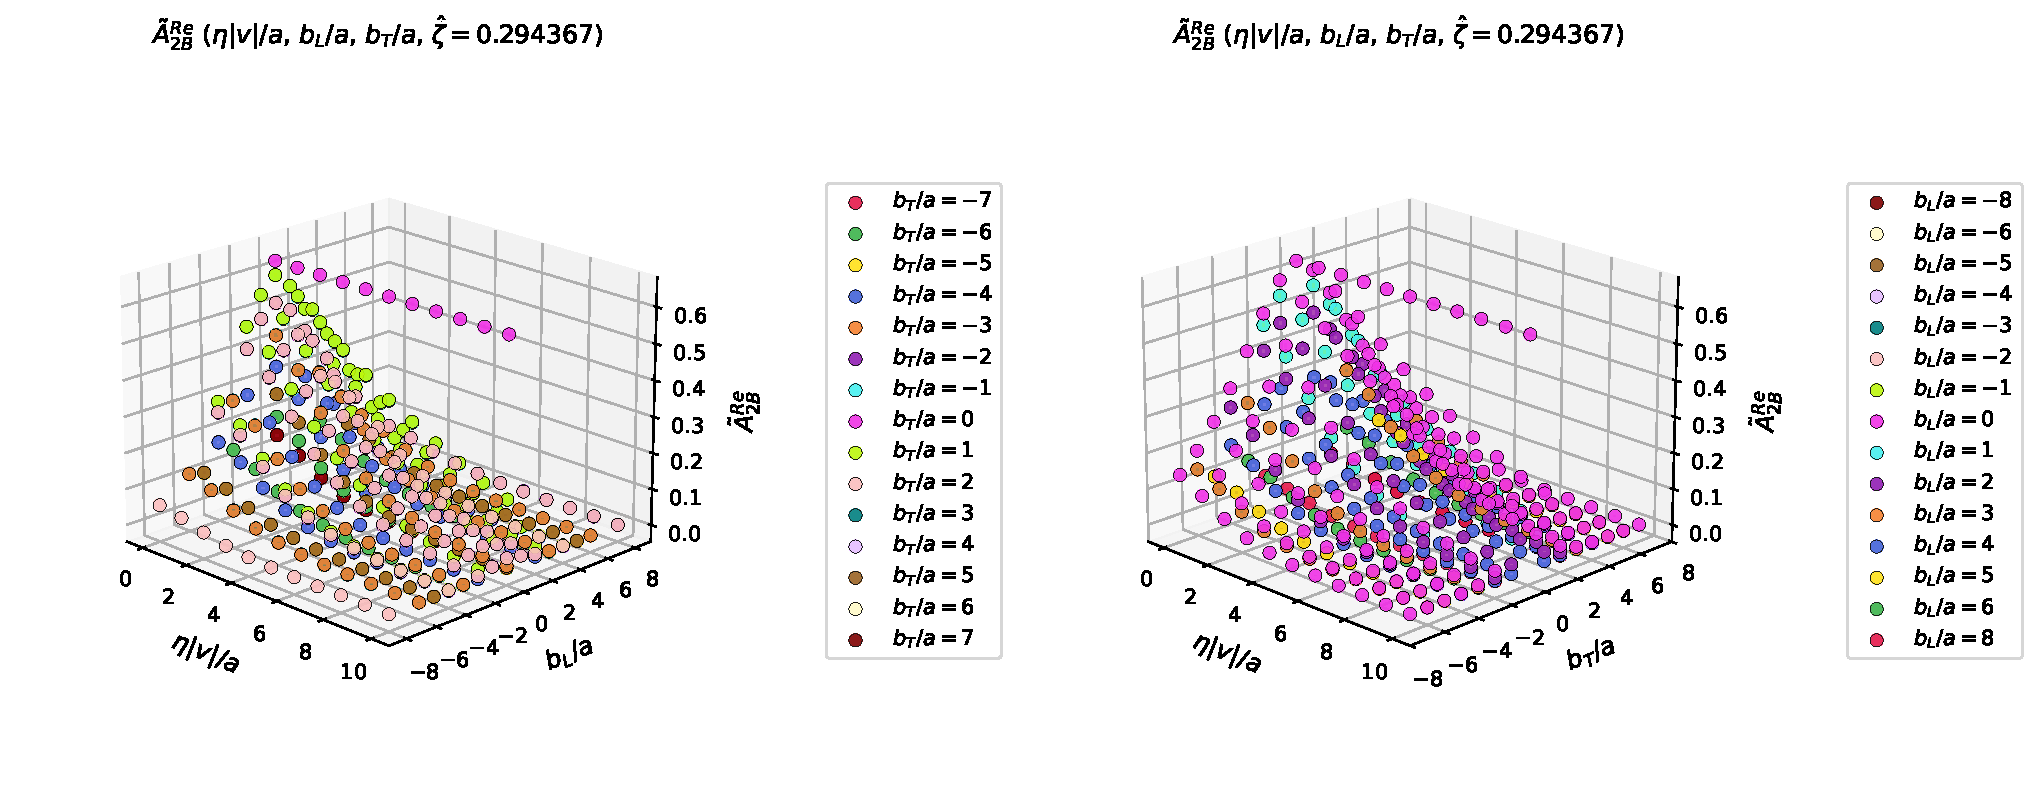
\includegraphics[width=0.98\linewidth,height=0.73\textheight,keepaspectratio]{ReA2B_PL-2_3D.pdf}\\[1mm]
{\small $\zetahat=0.294367$; $(b_L,b_T)$; staple-length dependence}
\figsrc{Thesis, Ch. 5: raw amplitude profiles; complete original panels.}
\end{frame}

\begin{frame}{$\tAmp_{2B}^{\mathrm{Re}}$ at $P_L=-2$: invariant coordinates}
\centering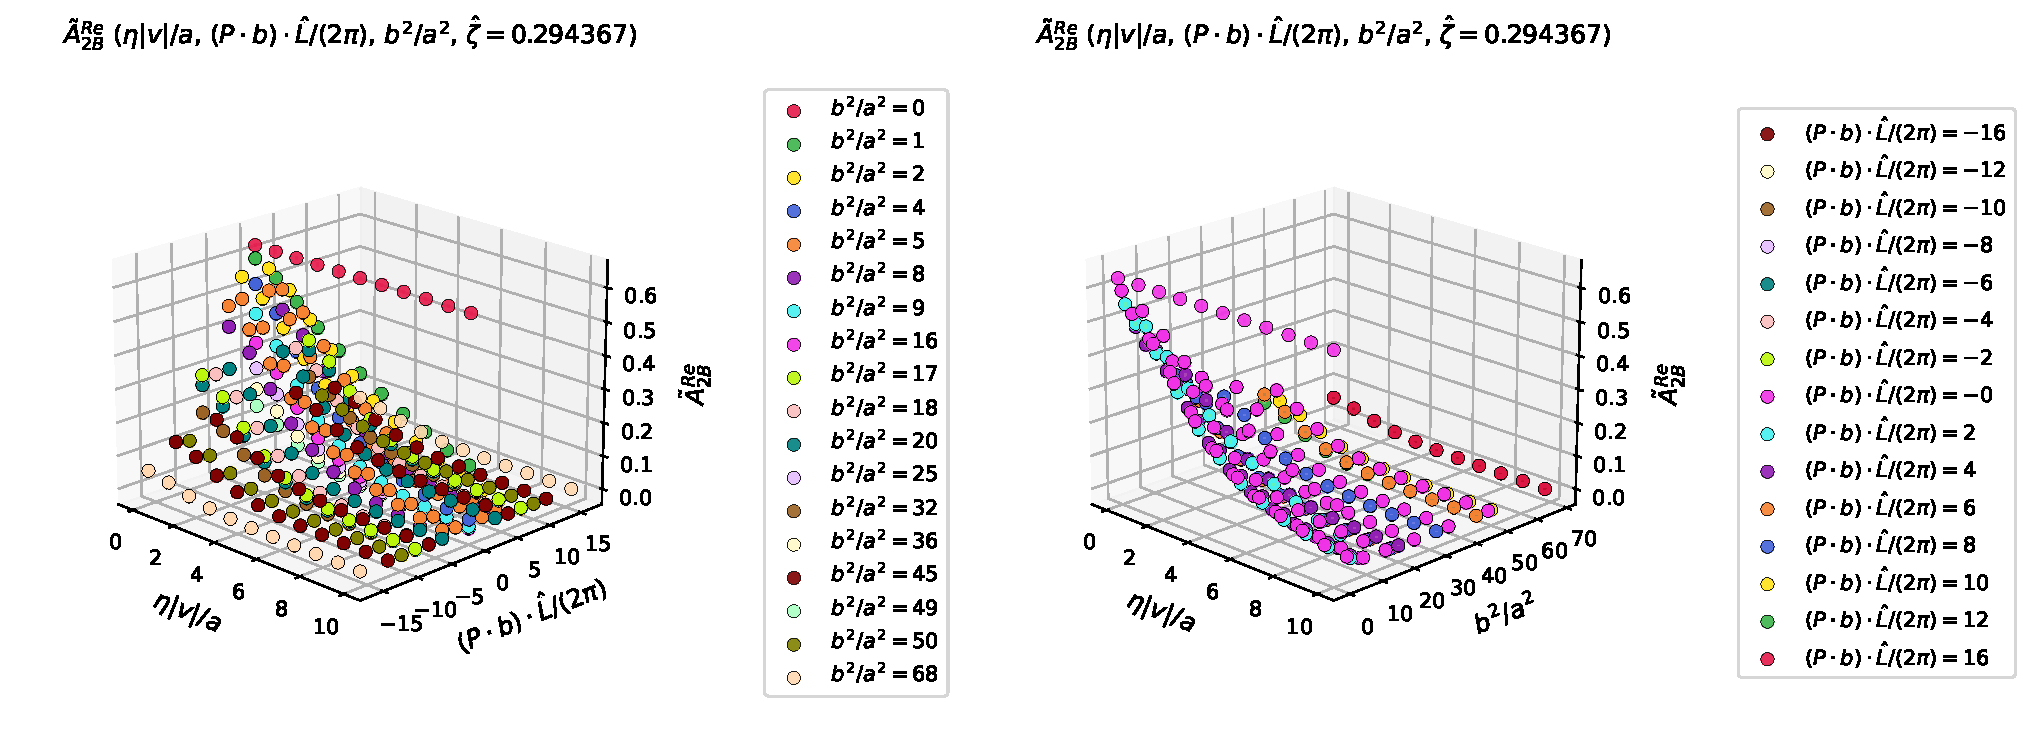
\includegraphics[width=0.98\linewidth,height=0.73\textheight,keepaspectratio]{ReA2B_Pb_bsq_PL-2_3D.pdf}\\[1mm]
{\small $\zetahat=0.294367$; $(\nu,s)$; staple-length dependence}
\figsrc{Thesis, Ch. 5: raw amplitude profiles; complete original panels.}
\end{frame}

\begin{frame}{$\tAmp_{2B}^{\mathrm{Im}}$ at $P_L=-2$: lattice coordinates}
\centering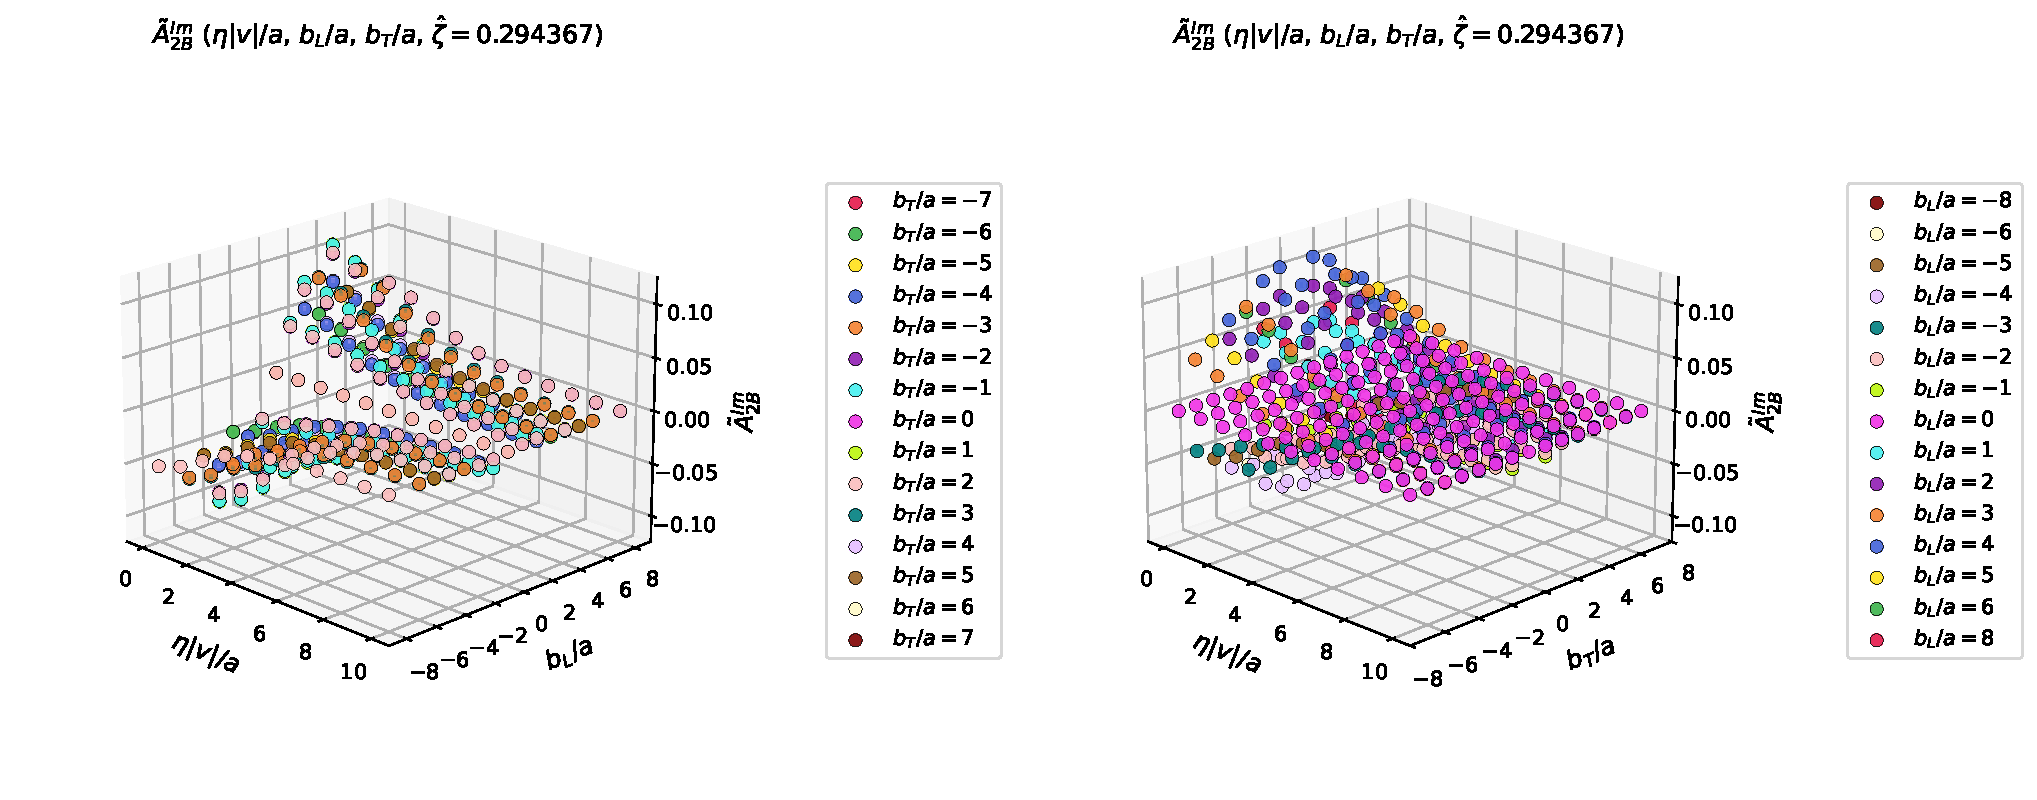
\includegraphics[width=0.98\linewidth,height=0.73\textheight,keepaspectratio]{ImA2B_PL-2_3D.pdf}\\[1mm]
{\small $\zetahat=0.294367$; $(b_L,b_T)$; staple-length dependence}
\figsrc{Thesis, Ch. 5: raw amplitude profiles; complete original panels.}
\end{frame}

\begin{frame}{$\tAmp_{2B}^{\mathrm{Im}}$ at $P_L=-2$: invariant coordinates}
\centering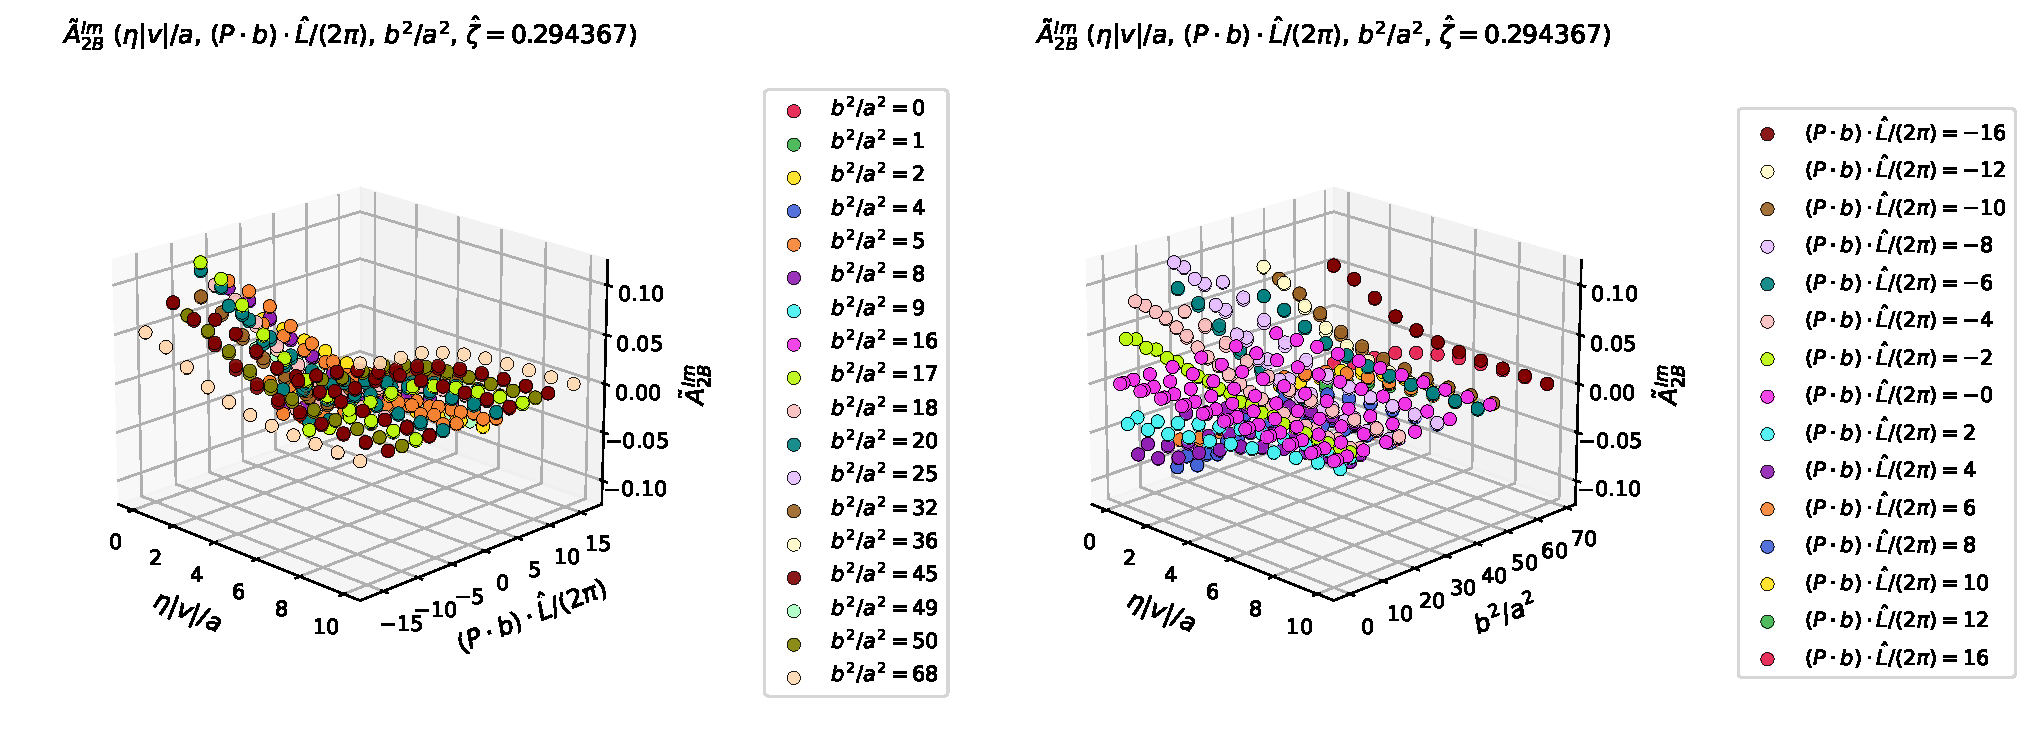
\includegraphics[width=0.98\linewidth,height=0.73\textheight,keepaspectratio]{ImA2B_Pb_bsq_PL-2_3D.pdf}\\[1mm]
{\small $\zetahat=0.294367$; $(\nu,s)$; staple-length dependence}
\figsrc{Thesis, Ch. 5: raw amplitude profiles; complete original panels.}
\end{frame}

\begin{frame}{$\tAmp_{12B}^{\mathrm{Re}}$ at $P_L=-2$: lattice coordinates}
\centering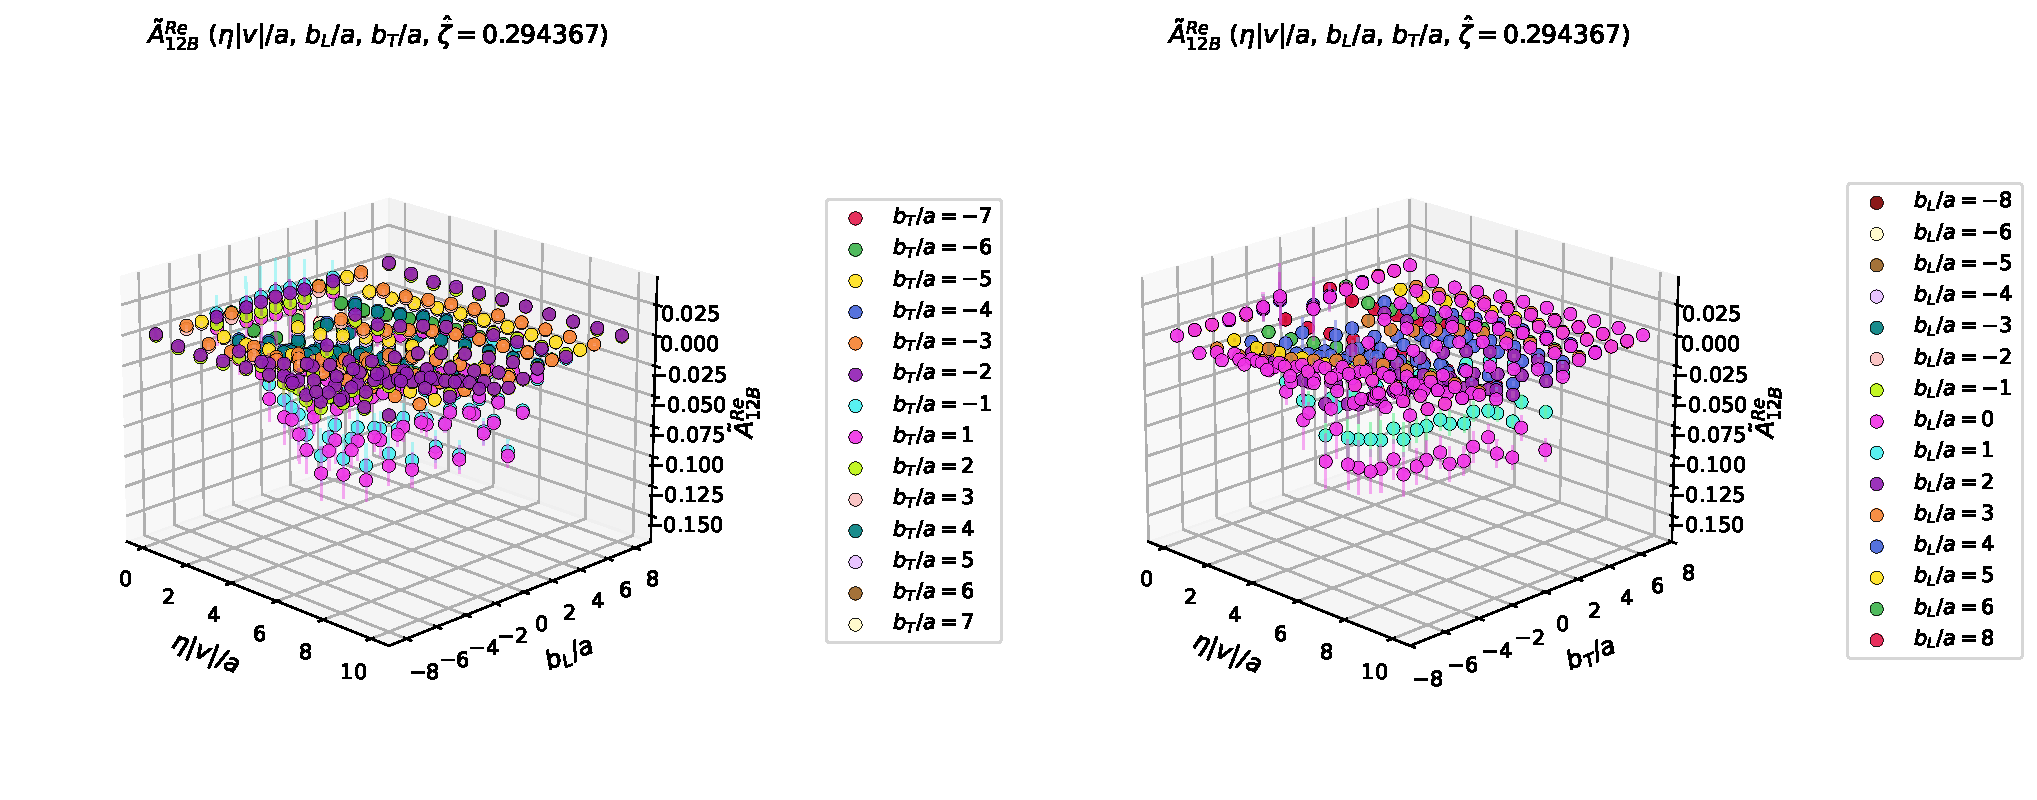
\includegraphics[width=0.98\linewidth,height=0.73\textheight,keepaspectratio]{ReA12B_PL-2_3D.pdf}\\[1mm]
{\small $\zetahat=0.294367$; $(b_L,b_T)$; staple-length dependence}
\figsrc{Thesis, Ch. 5: raw amplitude profiles; complete original panels.}
\end{frame}

\begin{frame}{$\tAmp_{12B}^{\mathrm{Re}}$ at $P_L=-2$: invariant coordinates}
\centering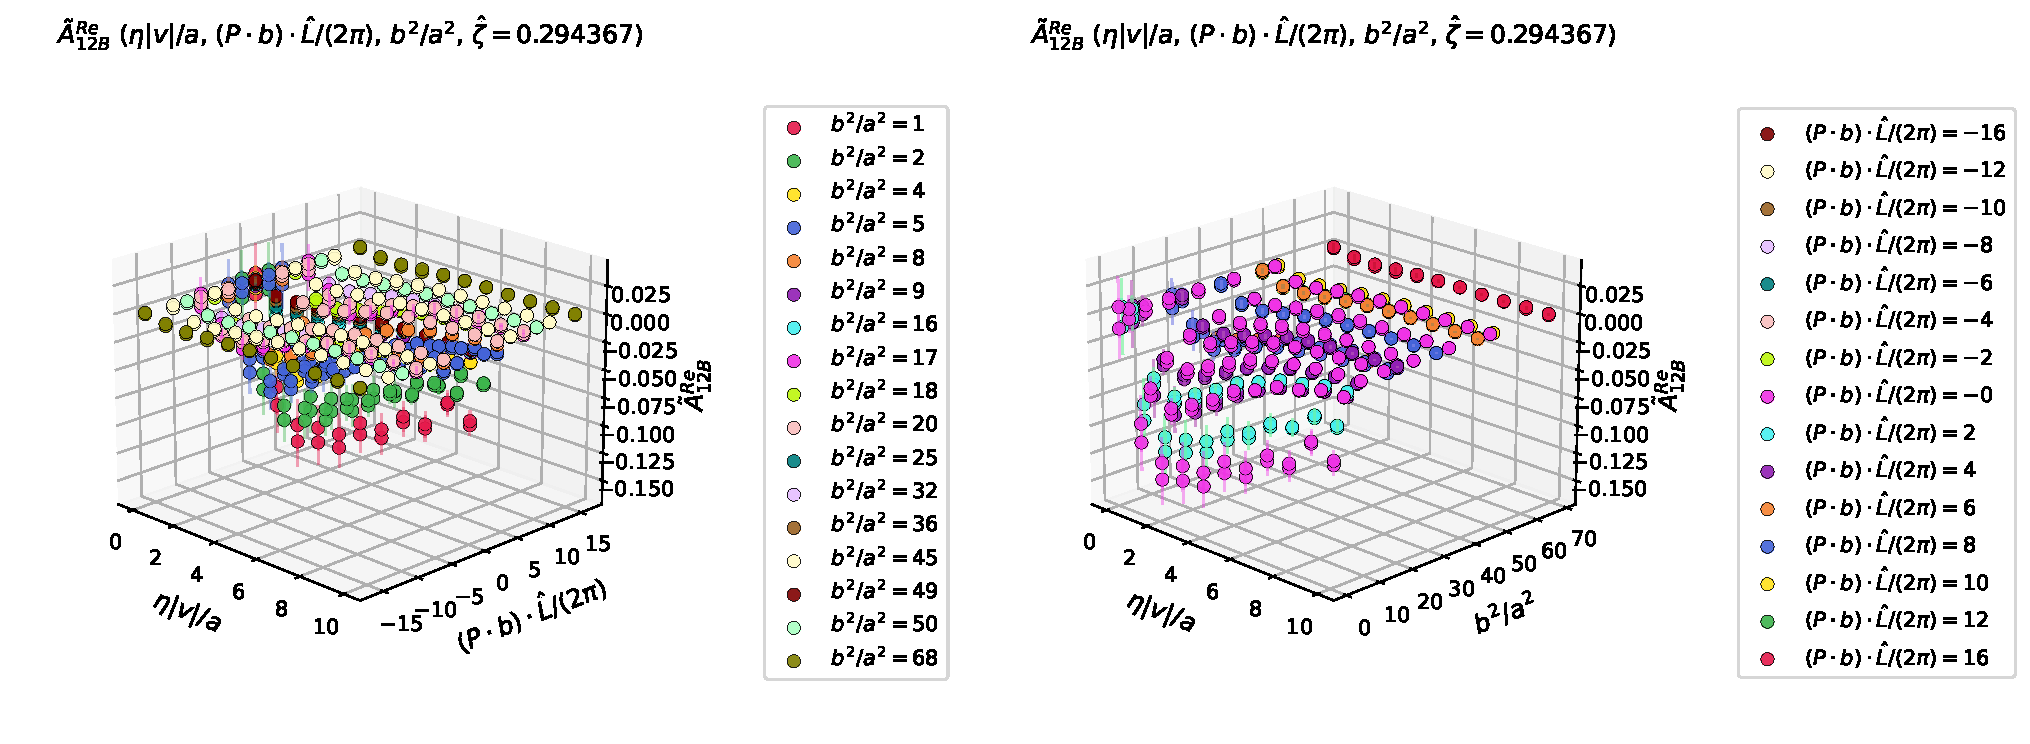
\includegraphics[width=0.98\linewidth,height=0.73\textheight,keepaspectratio]{ReA12B_Pb_bsq_PL-2_3D.pdf}\\[1mm]
{\small $\zetahat=0.294367$; $(\nu,s)$; staple-length dependence}
\figsrc{Thesis, Ch. 5: raw amplitude profiles; complete original panels.}
\end{frame}

\begin{frame}{$\tAmp_{12B}^{\mathrm{Im}}$ at $P_L=-2$: lattice coordinates}
\centering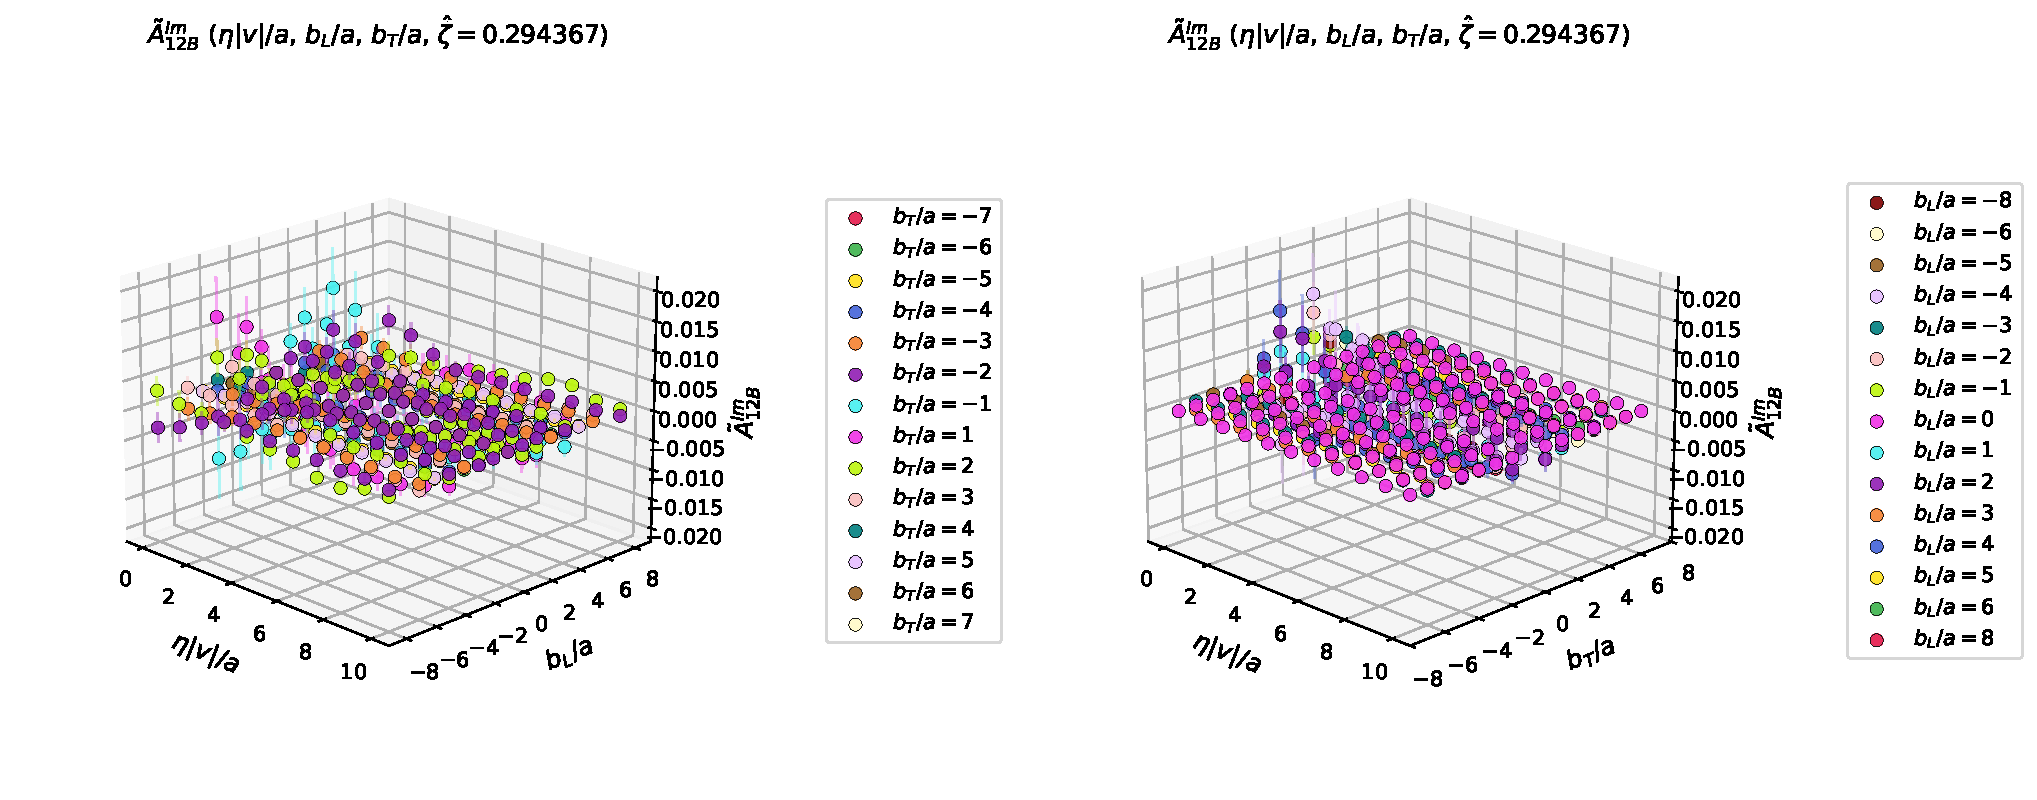
\includegraphics[width=0.98\linewidth,height=0.73\textheight,keepaspectratio]{ImA12B_PL-2_3D.pdf}\\[1mm]
{\small $\zetahat=0.294367$; $(b_L,b_T)$; staple-length dependence}
\figsrc{Thesis, Ch. 5: raw amplitude profiles; complete original panels.}
\end{frame}

\begin{frame}{$\tAmp_{12B}^{\mathrm{Im}}$ at $P_L=-2$: invariant coordinates}
\centering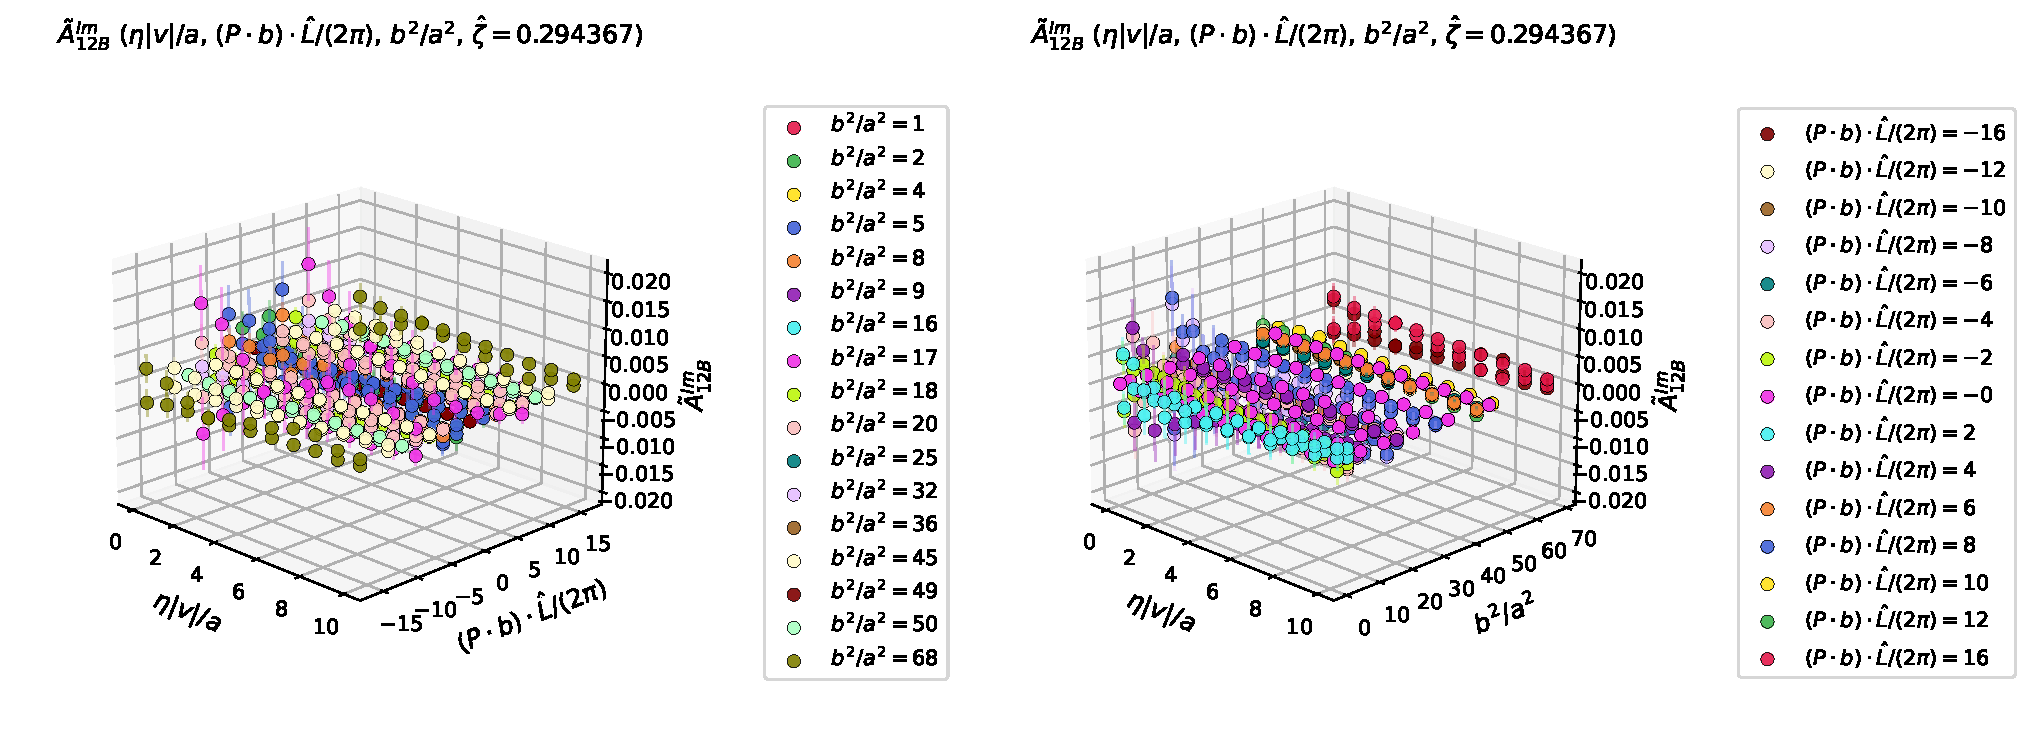
\includegraphics[width=0.98\linewidth,height=0.73\textheight,keepaspectratio]{ImA12B_Pb_bsq_PL-2_3D.pdf}\\[1mm]
{\small $\zetahat=0.294367$; $(\nu,s)$; staple-length dependence}
\figsrc{Thesis, Ch. 5: raw amplitude profiles; complete original panels.}
\end{frame}

\begin{frame}{$\tAmp_{2B}^{\mathrm{Re}}$ at $P_L=-2$: lattice coordinates}
\centering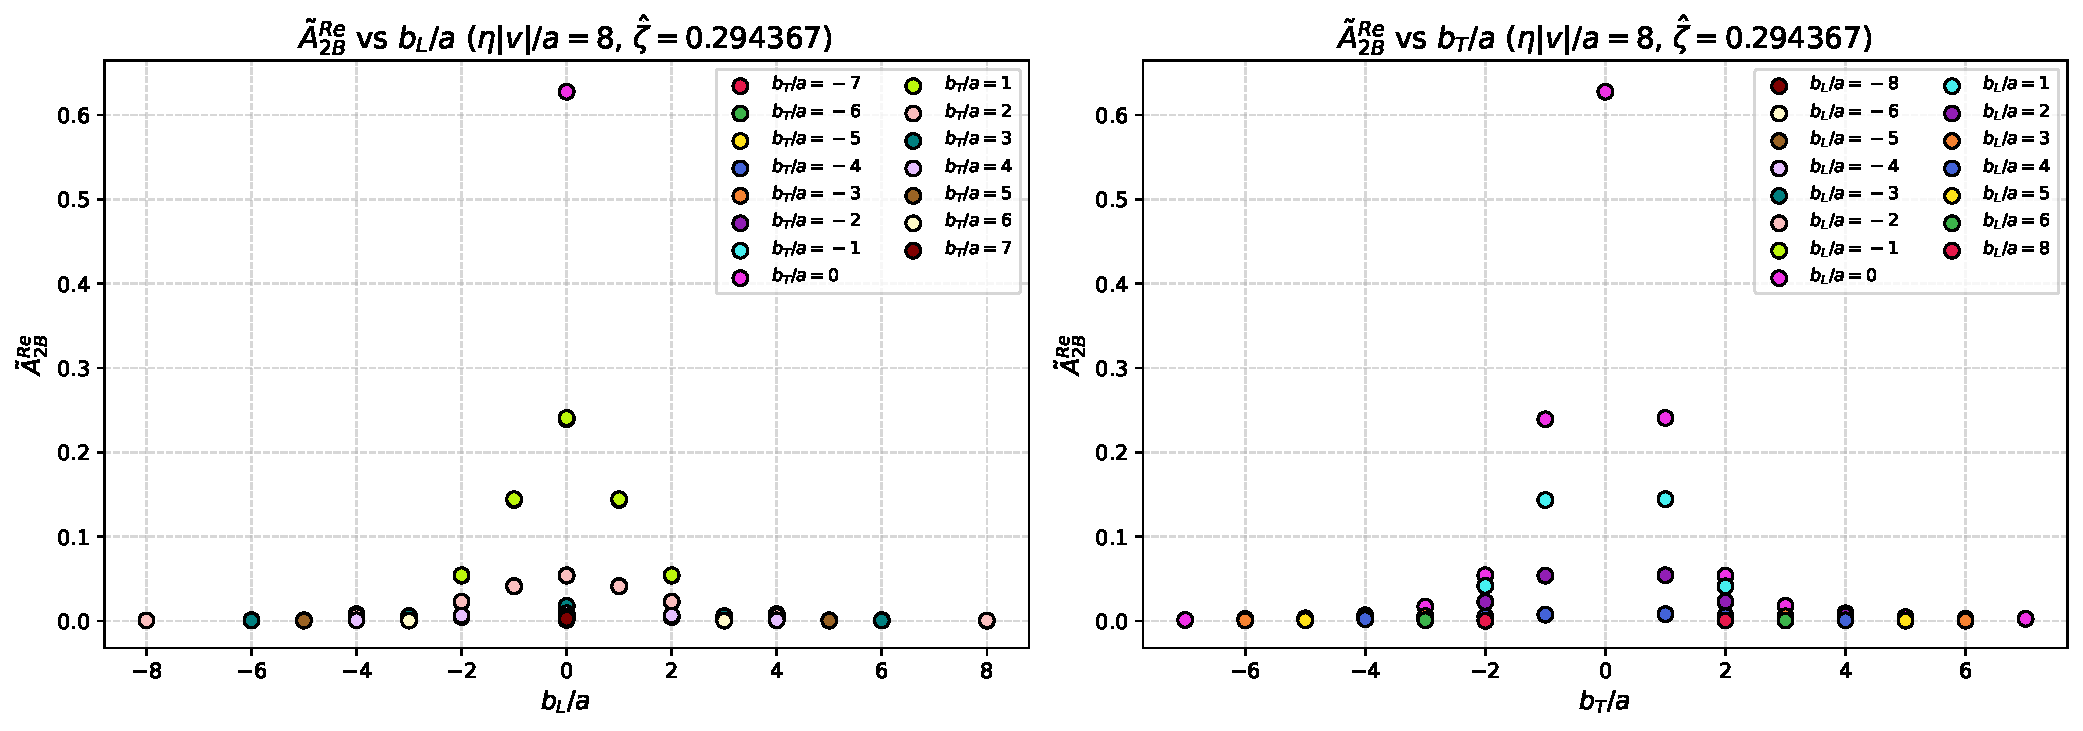
\includegraphics[width=0.98\linewidth,height=0.73\textheight,keepaspectratio]{ReA2B_eta8_PL-2_2D.pdf}\\[1mm]
{\small $\zetahat=0.294367$; $(b_L,b_T)$; $\eta|v|/a=8$ slices}
\figsrc{Thesis, Ch. 5: raw amplitude profiles; complete original panels.}
\end{frame}

\begin{frame}{$\tAmp_{2B}^{\mathrm{Re}}$ at $P_L=-2$: invariant coordinates}
\centering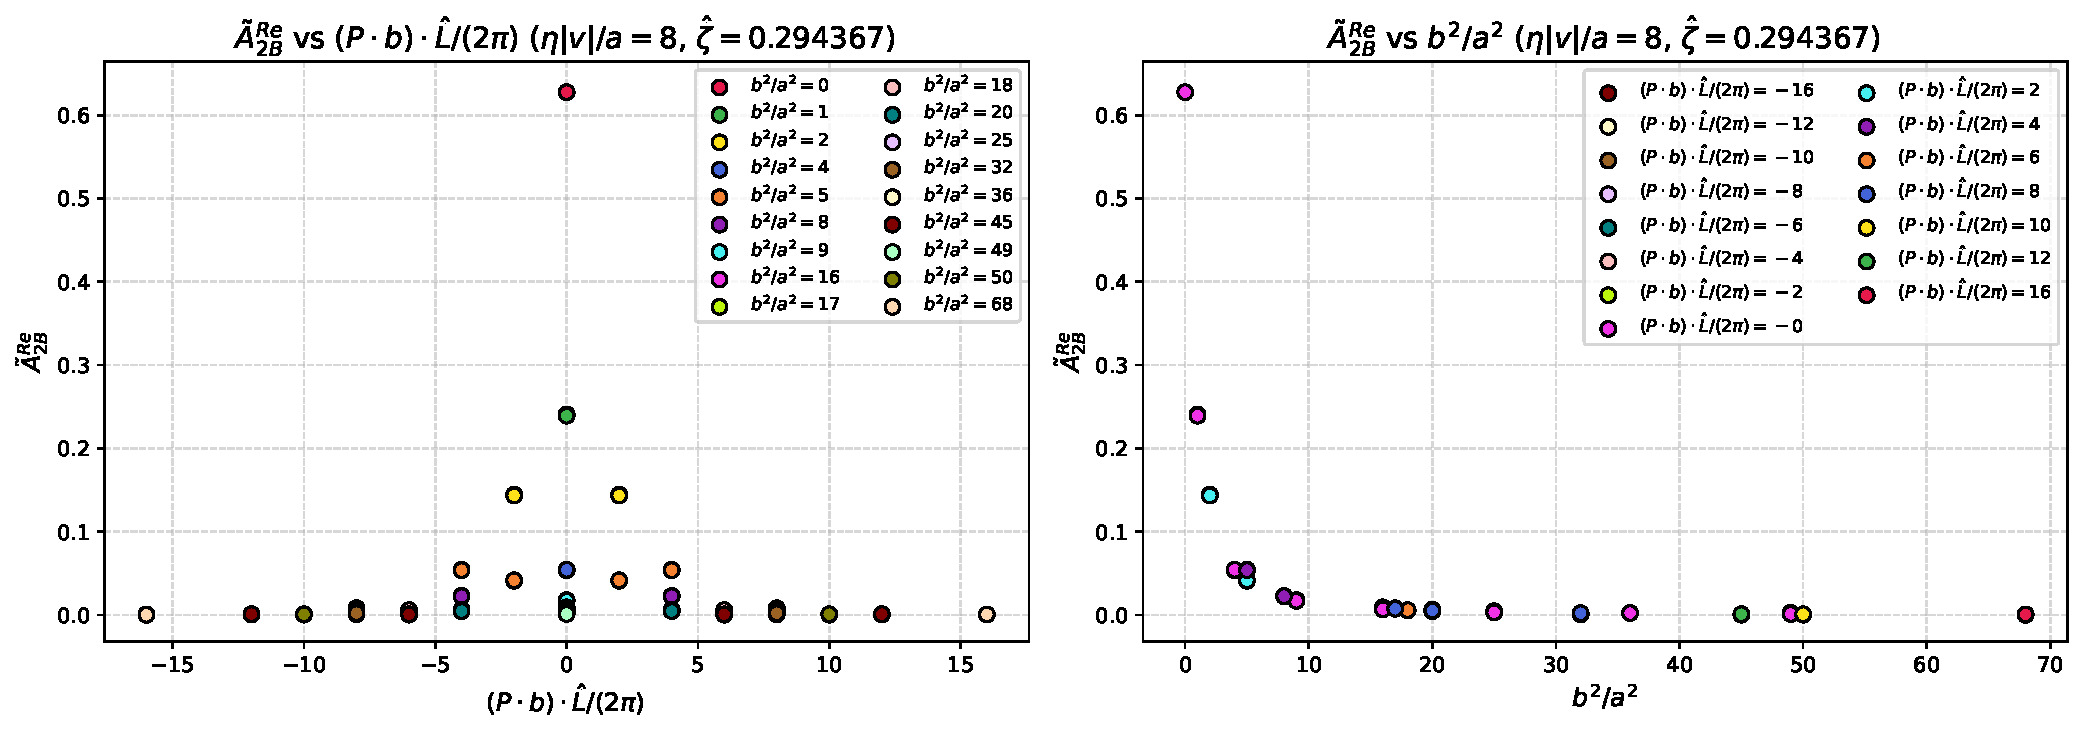
\includegraphics[width=0.98\linewidth,height=0.73\textheight,keepaspectratio]{ReA2B_Pb_bsq_eta8_PL-2_2D.pdf}\\[1mm]
{\small $\zetahat=0.294367$; $(\nu,s)$; $\eta|v|/a=8$ slices}
\figsrc{Thesis, Ch. 5: raw amplitude profiles; complete original panels.}
\end{frame}

\begin{frame}{$\tAmp_{2B}^{\mathrm{Im}}$ at $P_L=-2$: lattice coordinates}
\centering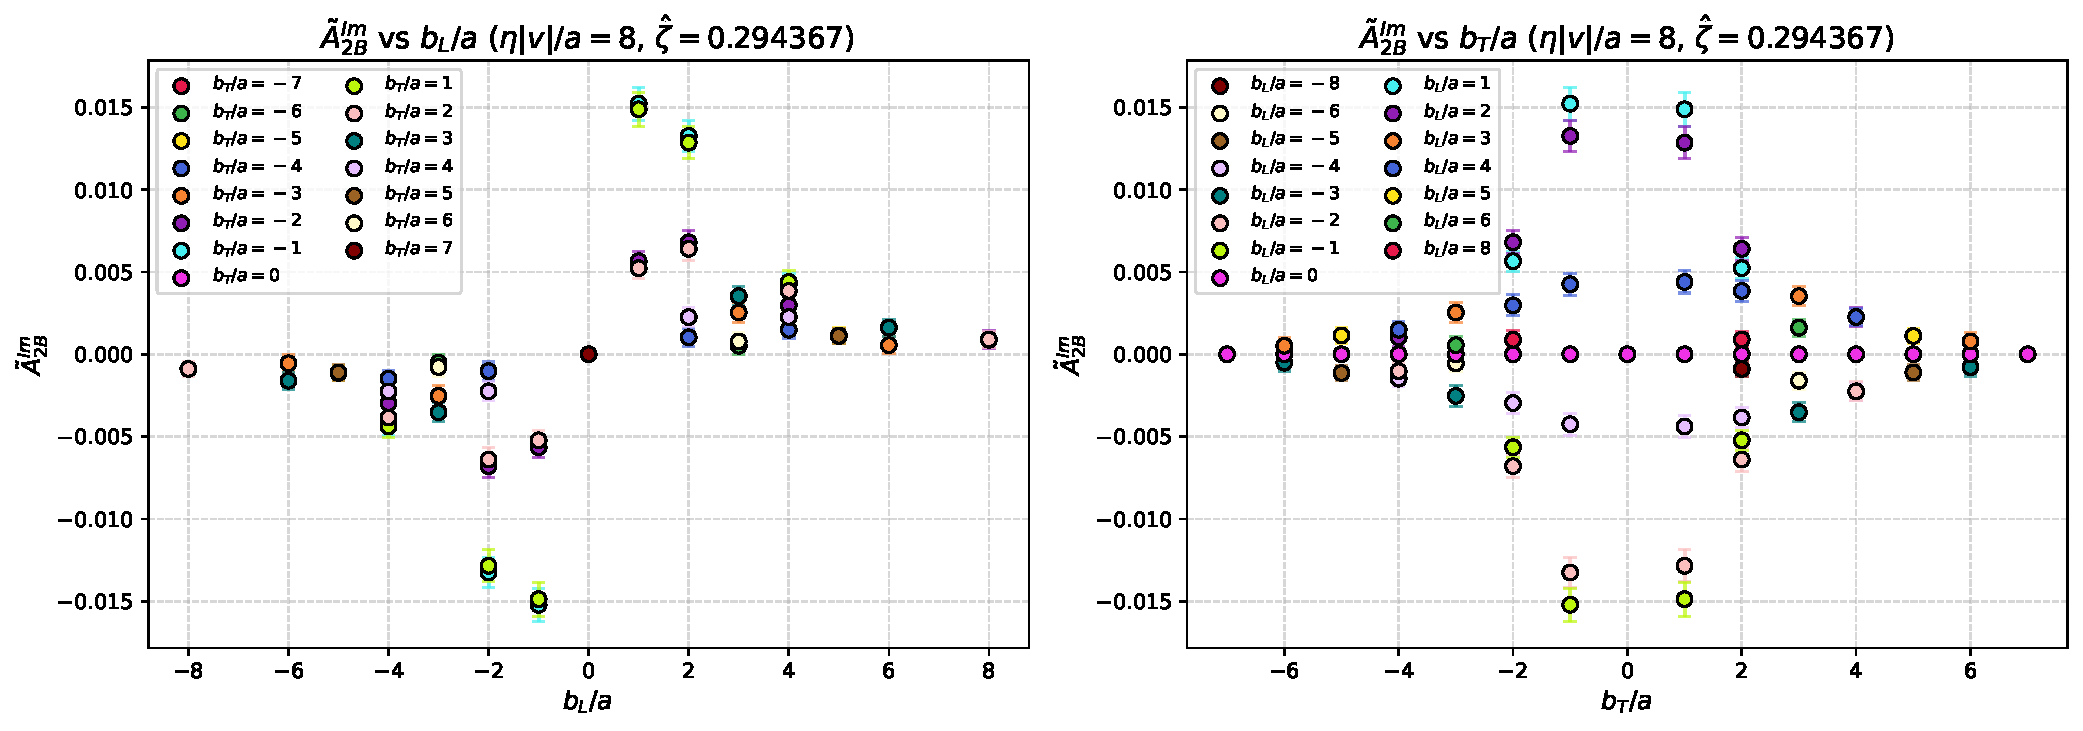
\includegraphics[width=0.98\linewidth,height=0.73\textheight,keepaspectratio]{ImA2B_eta8_PL-2_2D.pdf}\\[1mm]
{\small $\zetahat=0.294367$; $(b_L,b_T)$; $\eta|v|/a=8$ slices}
\figsrc{Thesis, Ch. 5: raw amplitude profiles; complete original panels.}
\end{frame}

\begin{frame}{$\tAmp_{2B}^{\mathrm{Im}}$ at $P_L=-2$: invariant coordinates}
\centering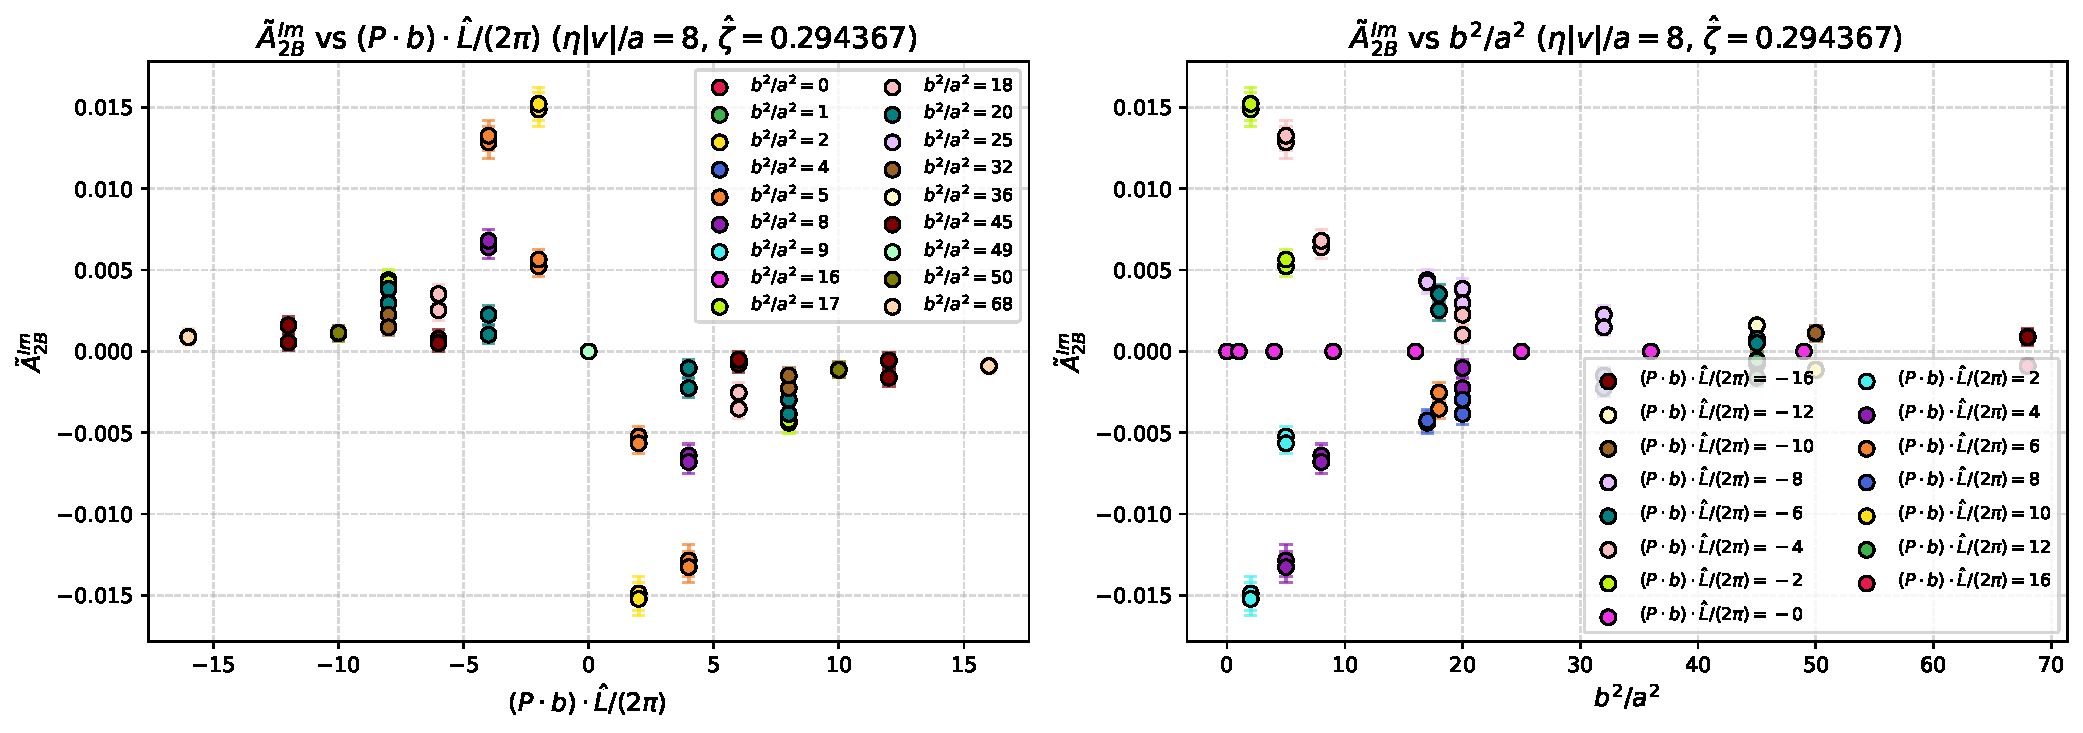
\includegraphics[width=0.98\linewidth,height=0.73\textheight,keepaspectratio]{ImA2B_Pb_bsq_eta8_PL-2_2D.pdf}\\[1mm]
{\small $\zetahat=0.294367$; $(\nu,s)$; $\eta|v|/a=8$ slices}
\figsrc{Thesis, Ch. 5: raw amplitude profiles; complete original panels.}
\end{frame}

\begin{frame}{$\tAmp_{12B}^{\mathrm{Re}}$ at $P_L=-2$: lattice coordinates}
\centering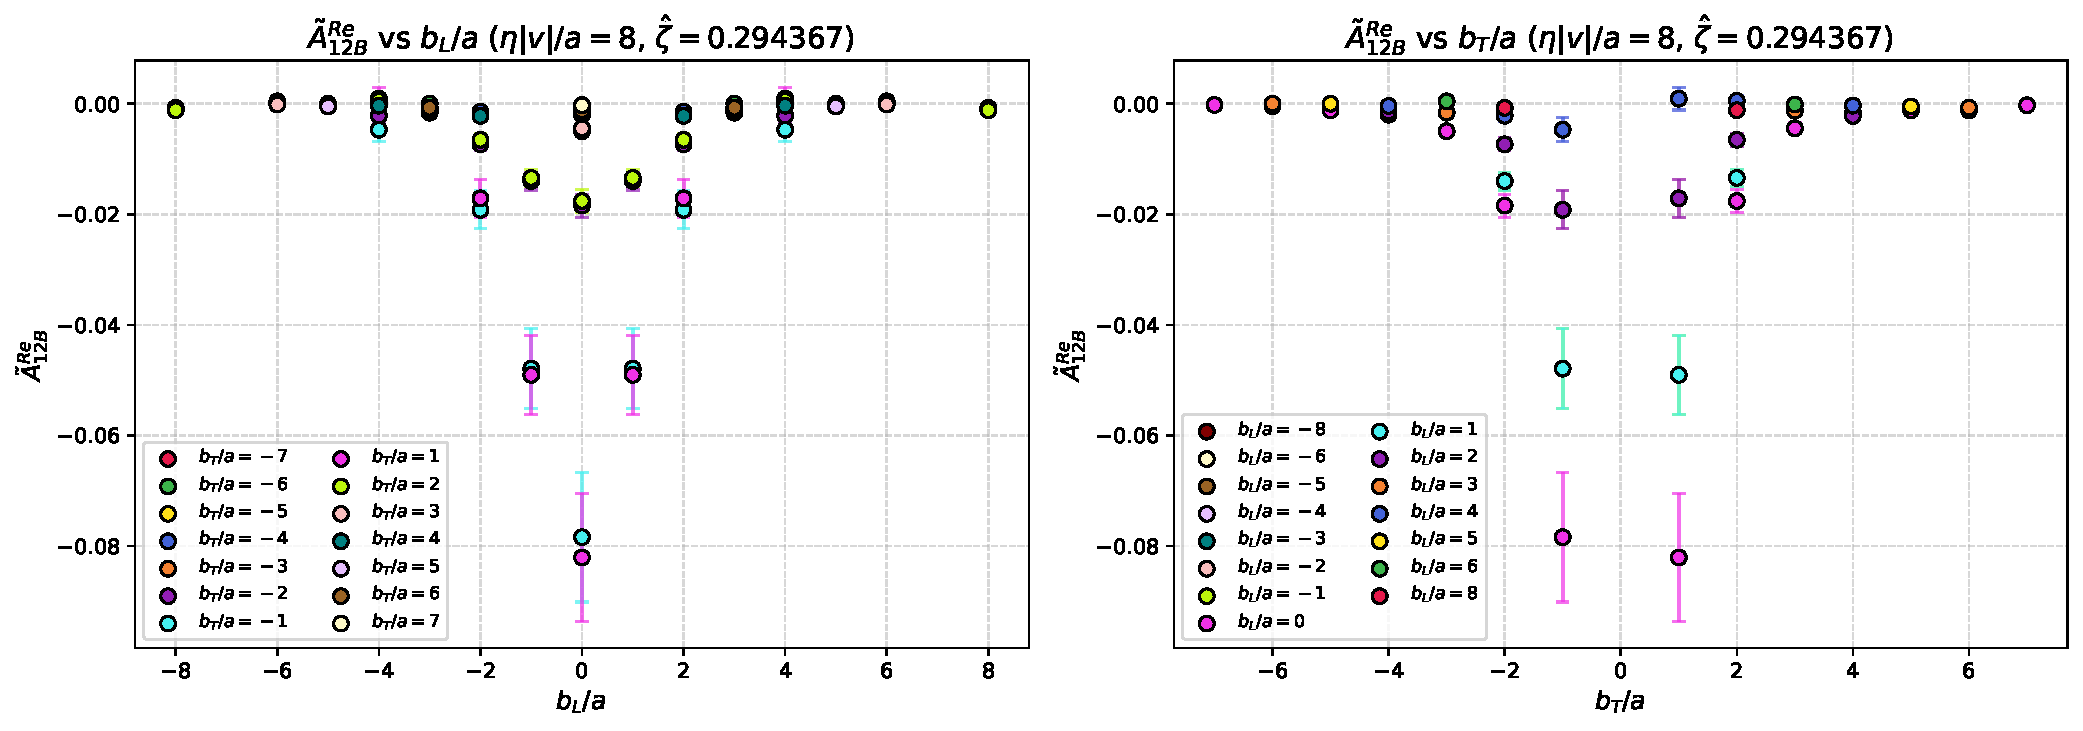
\includegraphics[width=0.98\linewidth,height=0.73\textheight,keepaspectratio]{ReA12B_eta8_PL-2_2D.pdf}\\[1mm]
{\small $\zetahat=0.294367$; $(b_L,b_T)$; $\eta|v|/a=8$ slices}
\figsrc{Thesis, Ch. 5: raw amplitude profiles; complete original panels.}
\end{frame}

\begin{frame}{$\tAmp_{12B}^{\mathrm{Re}}$ at $P_L=-2$: invariant coordinates}
\centering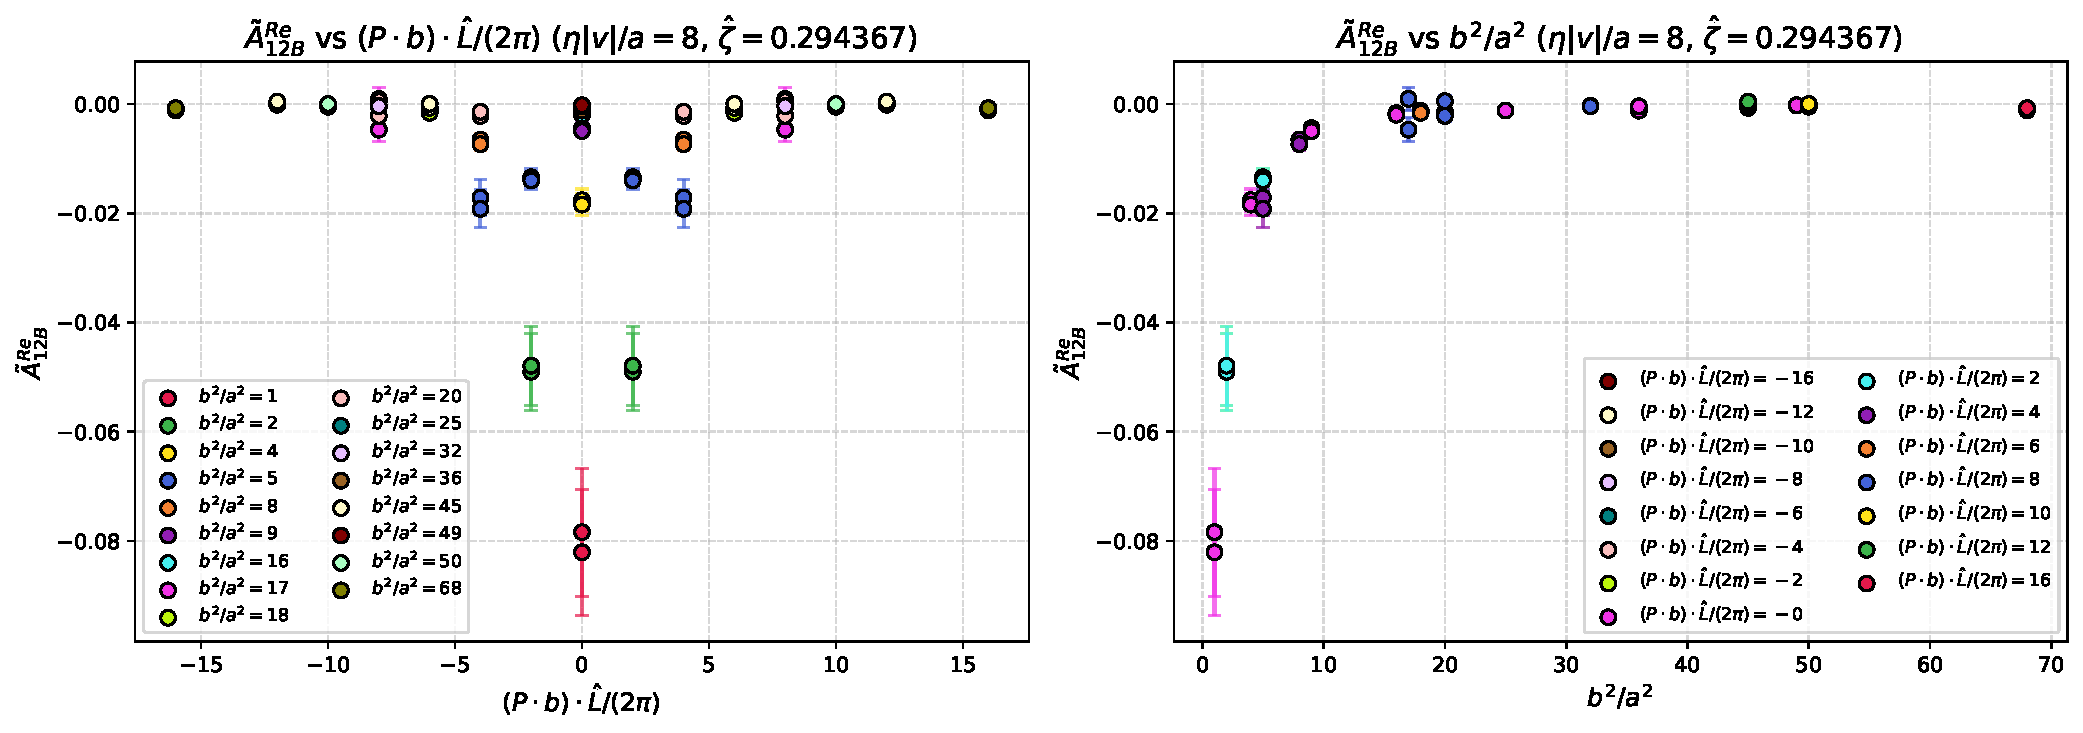
\includegraphics[width=0.98\linewidth,height=0.73\textheight,keepaspectratio]{ReA12B_Pb_bsq_eta8_PL-2_2D.pdf}\\[1mm]
{\small $\zetahat=0.294367$; $(\nu,s)$; $\eta|v|/a=8$ slices}
\figsrc{Thesis, Ch. 5: raw amplitude profiles; complete original panels.}
\end{frame}

\begin{frame}{$\tAmp_{12B}^{\mathrm{Im}}$ at $P_L=-2$: lattice coordinates}
\centering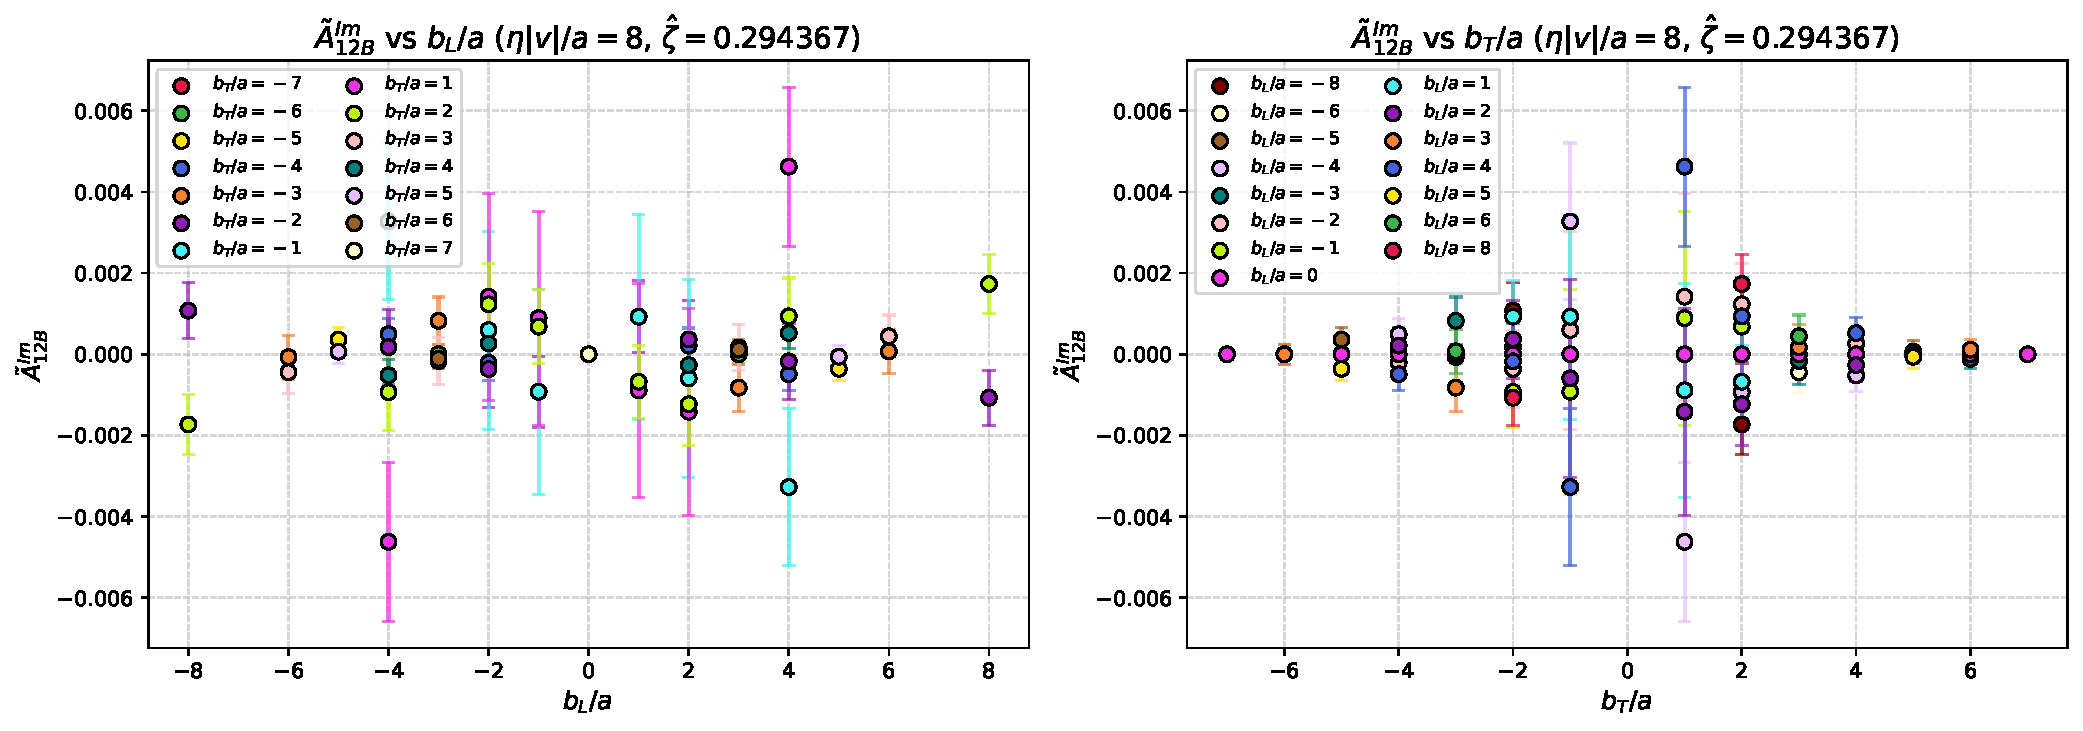
\includegraphics[width=0.98\linewidth,height=0.73\textheight,keepaspectratio]{ImA12B_eta8_PL-2_2D.pdf}\\[1mm]
{\small $\zetahat=0.294367$; $(b_L,b_T)$; $\eta|v|/a=8$ slices}
\figsrc{Thesis, Ch. 5: raw amplitude profiles; complete original panels.}
\end{frame}

\begin{frame}{$\tAmp_{12B}^{\mathrm{Im}}$ at $P_L=-2$: invariant coordinates}
\centering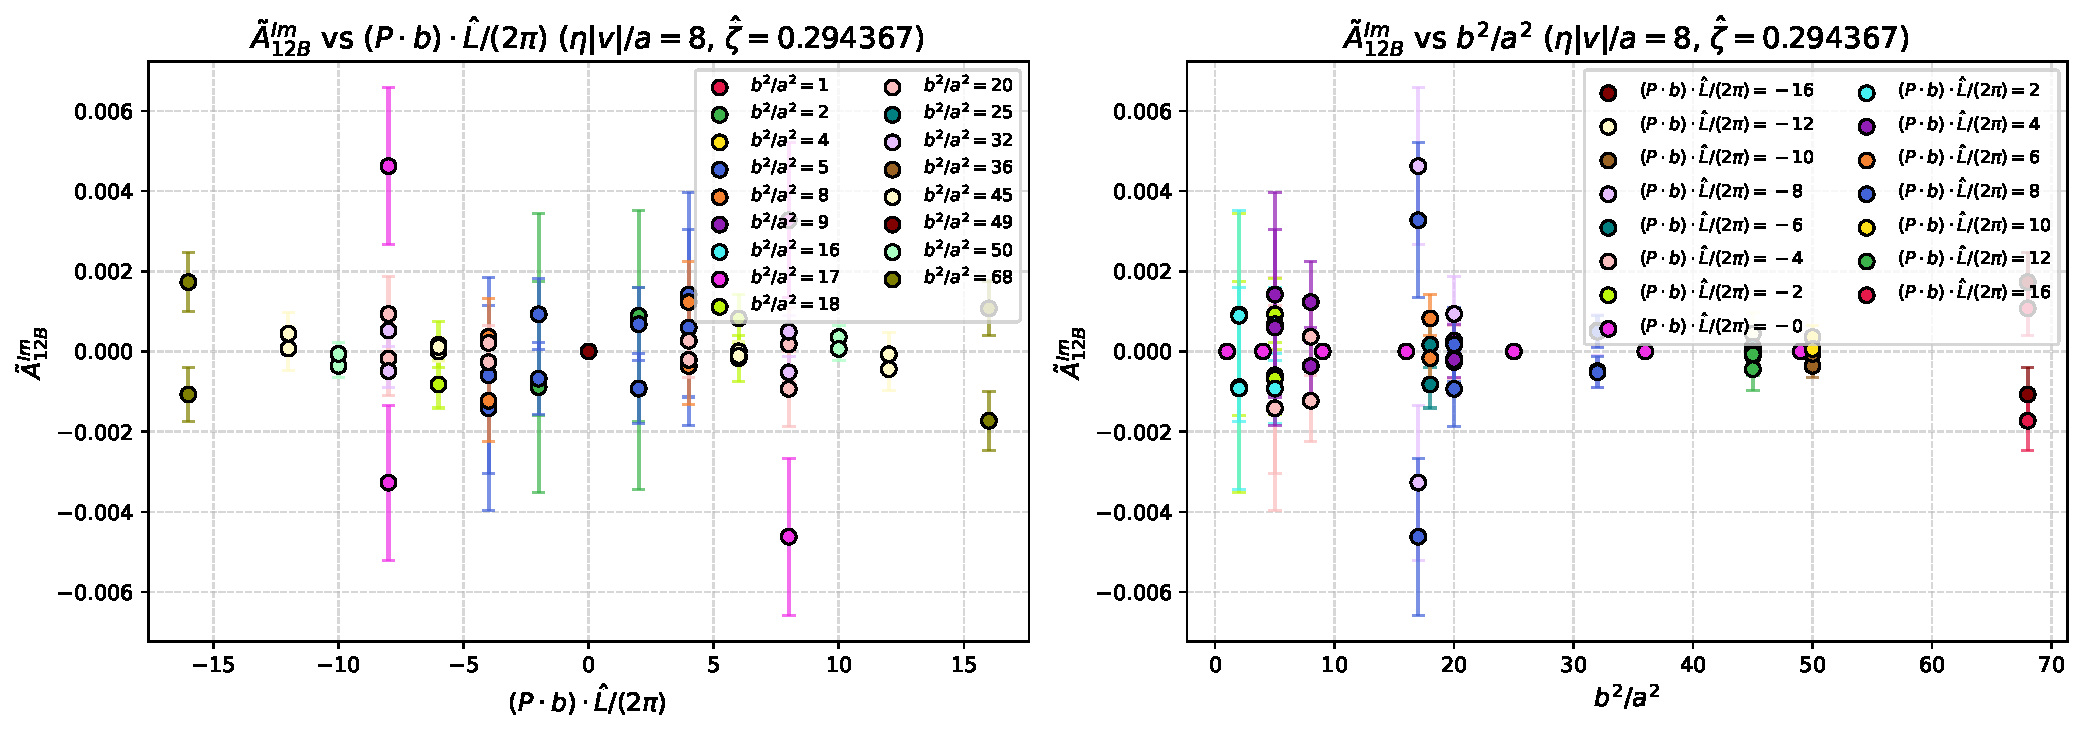
\includegraphics[width=0.98\linewidth,height=0.73\textheight,keepaspectratio]{ImA12B_Pb_bsq_eta8_PL-2_2D.pdf}\\[1mm]
{\small $\zetahat=0.294367$; $(\nu,s)$; $\eta|v|/a=8$ slices}
\figsrc{Thesis, Ch. 5: raw amplitude profiles; complete original panels.}
\end{frame}

\begin{frame}{$\tAmp_{2B}^{\mathrm{Re}}$ at $P_L=-3$: lattice coordinates}
\centering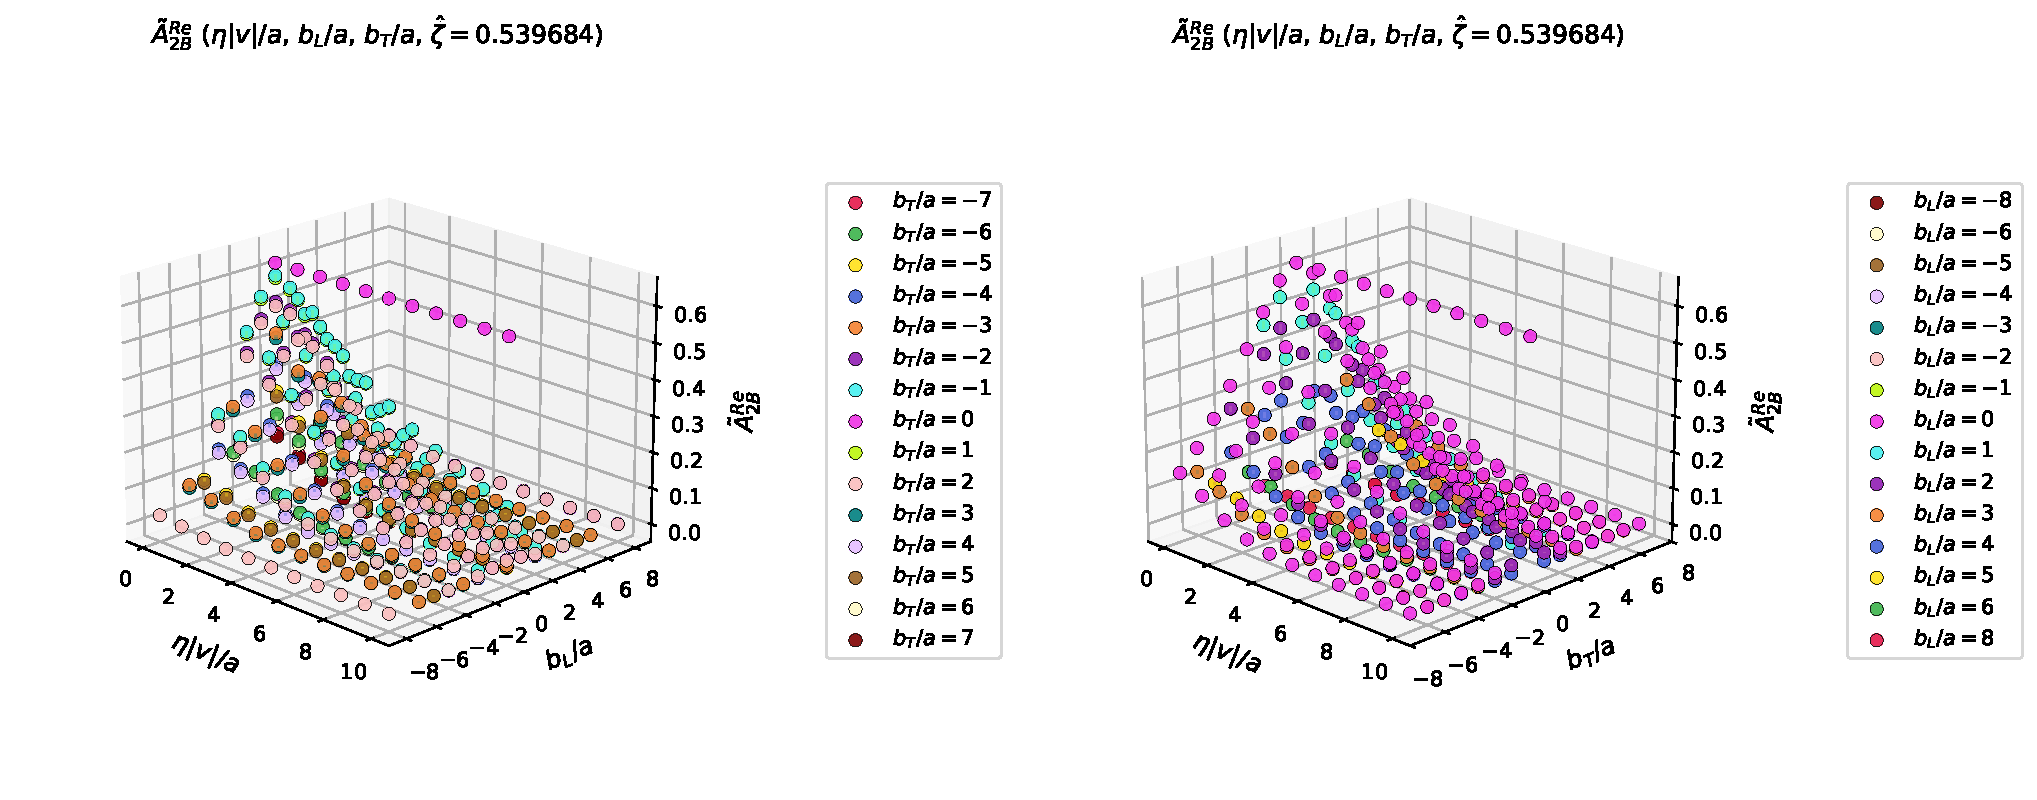
\includegraphics[width=0.98\linewidth,height=0.73\textheight,keepaspectratio]{ReA2B_PL-3_3D.pdf}\\[1mm]
{\small $\zetahat=0.539684$; $(b_L,b_T)$; staple-length dependence}
\figsrc{Thesis, Ch. 5: raw amplitude profiles; complete original panels.}
\end{frame}

\begin{frame}{$\tAmp_{2B}^{\mathrm{Re}}$ at $P_L=-3$: invariant coordinates}
\centering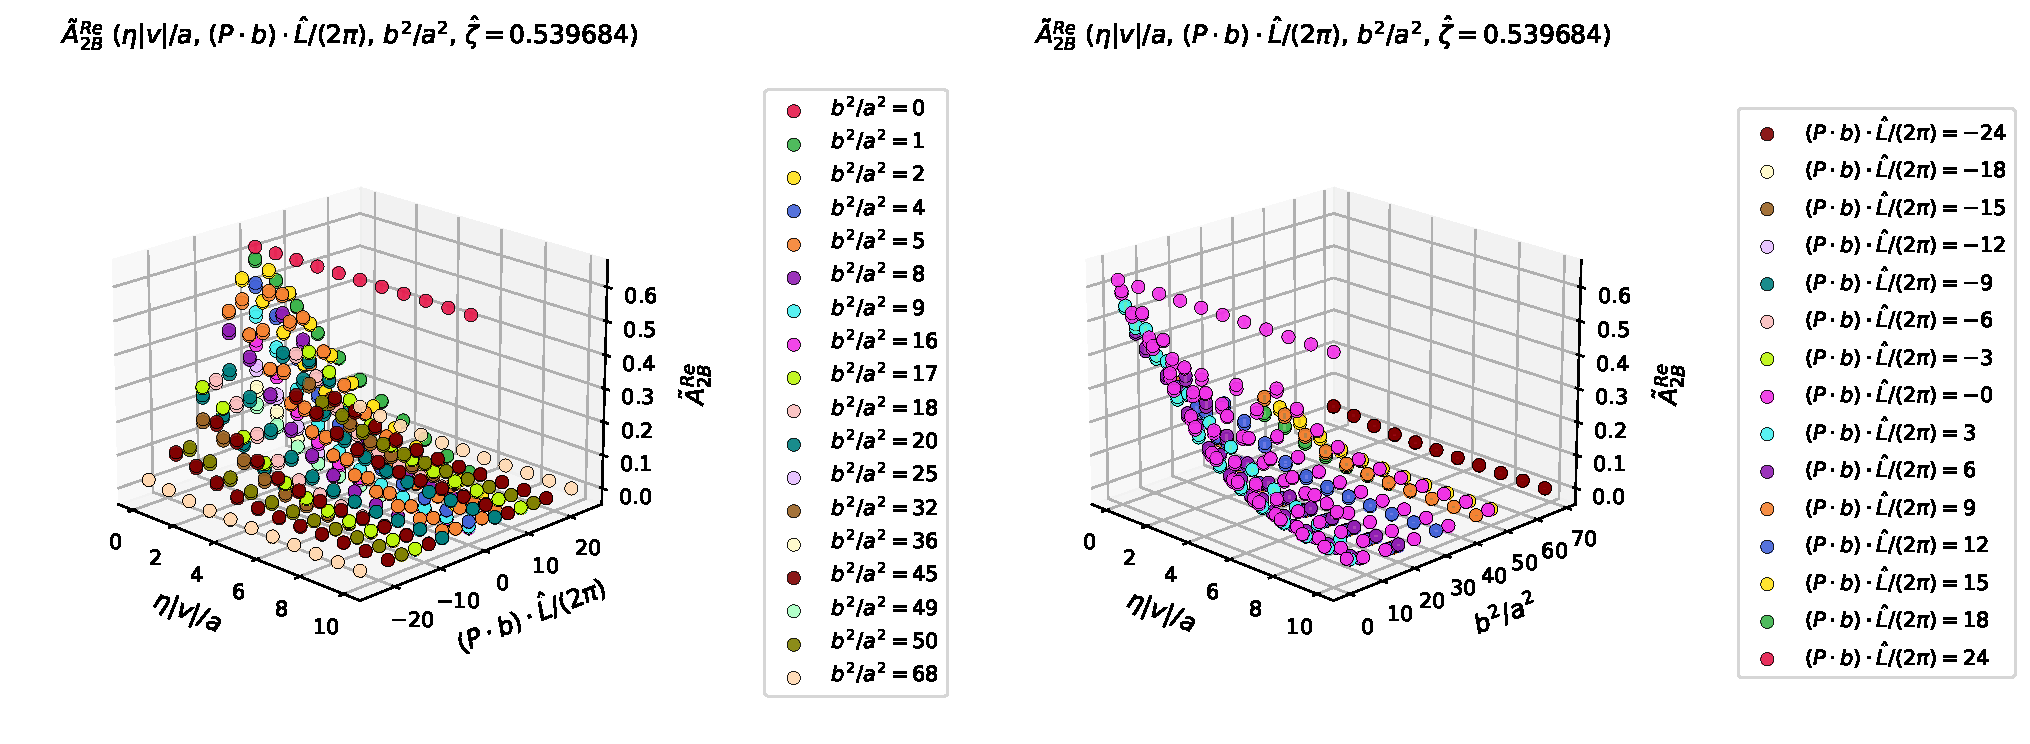
\includegraphics[width=0.98\linewidth,height=0.73\textheight,keepaspectratio]{ReA2B_Pb_bsq_PL-3_3D.pdf}\\[1mm]
{\small $\zetahat=0.539684$; $(\nu,s)$; staple-length dependence}
\figsrc{Thesis, Ch. 5: raw amplitude profiles; complete original panels.}
\end{frame}

\begin{frame}{$\tAmp_{2B}^{\mathrm{Im}}$ at $P_L=-3$: lattice coordinates}
\centering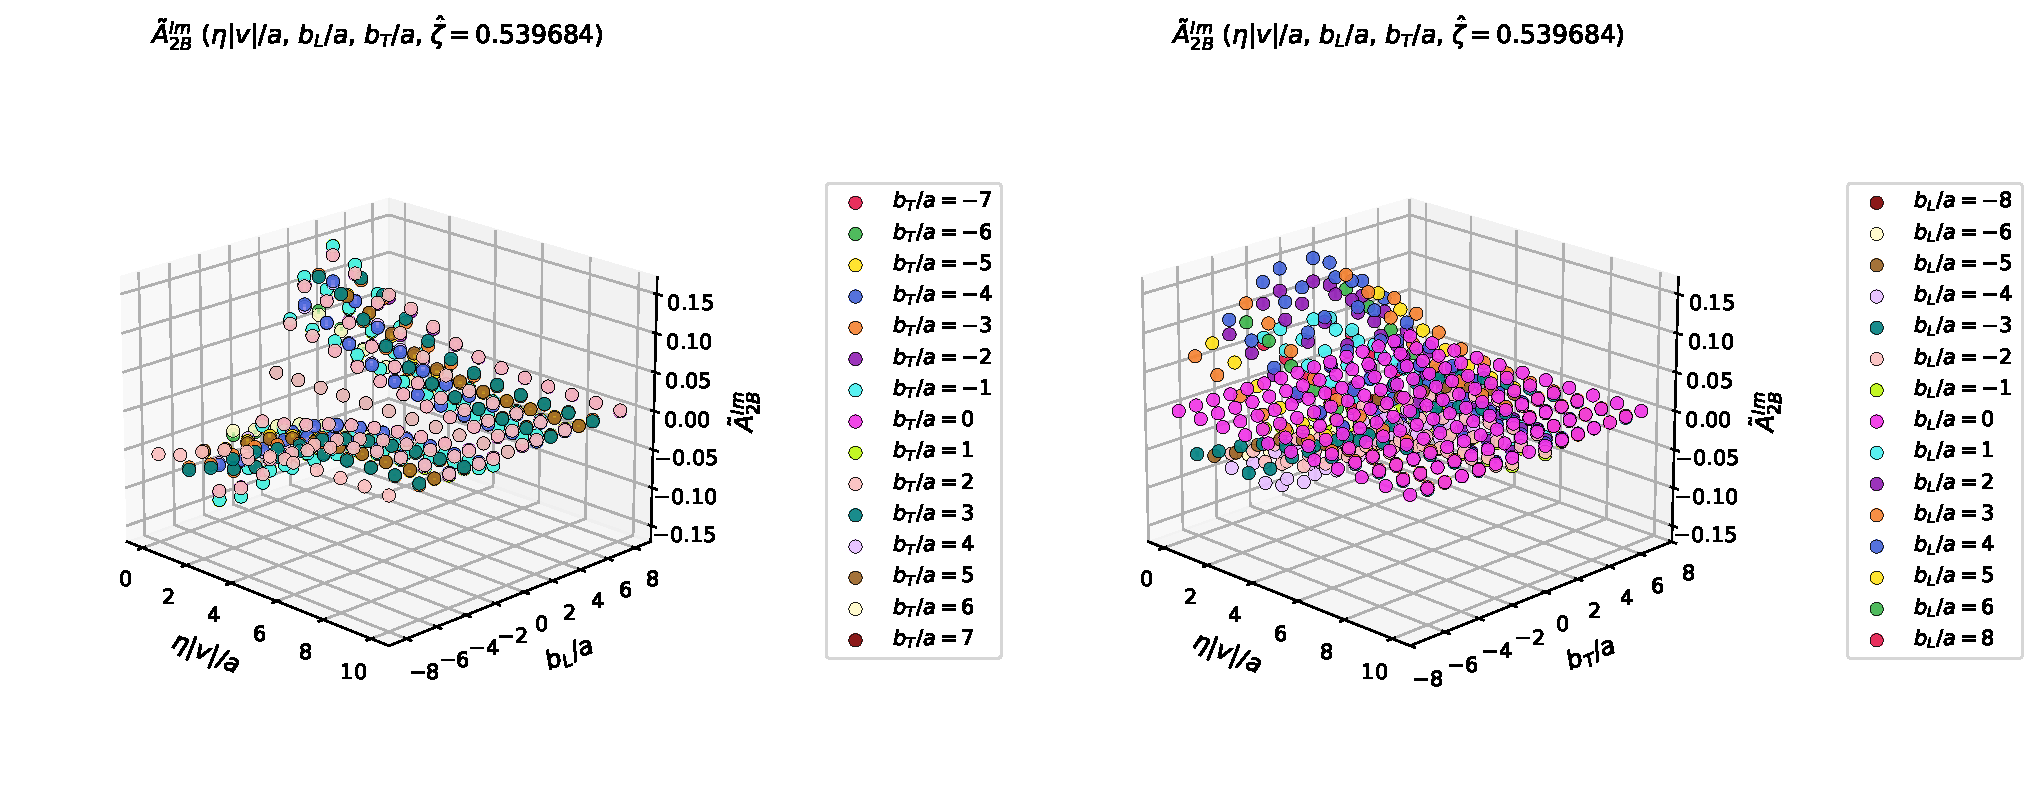
\includegraphics[width=0.98\linewidth,height=0.73\textheight,keepaspectratio]{ImA2B_PL-3_3D.pdf}\\[1mm]
{\small $\zetahat=0.539684$; $(b_L,b_T)$; staple-length dependence}
\figsrc{Thesis, Ch. 5: raw amplitude profiles; complete original panels.}
\end{frame}

\begin{frame}{$\tAmp_{2B}^{\mathrm{Im}}$ at $P_L=-3$: invariant coordinates}
\centering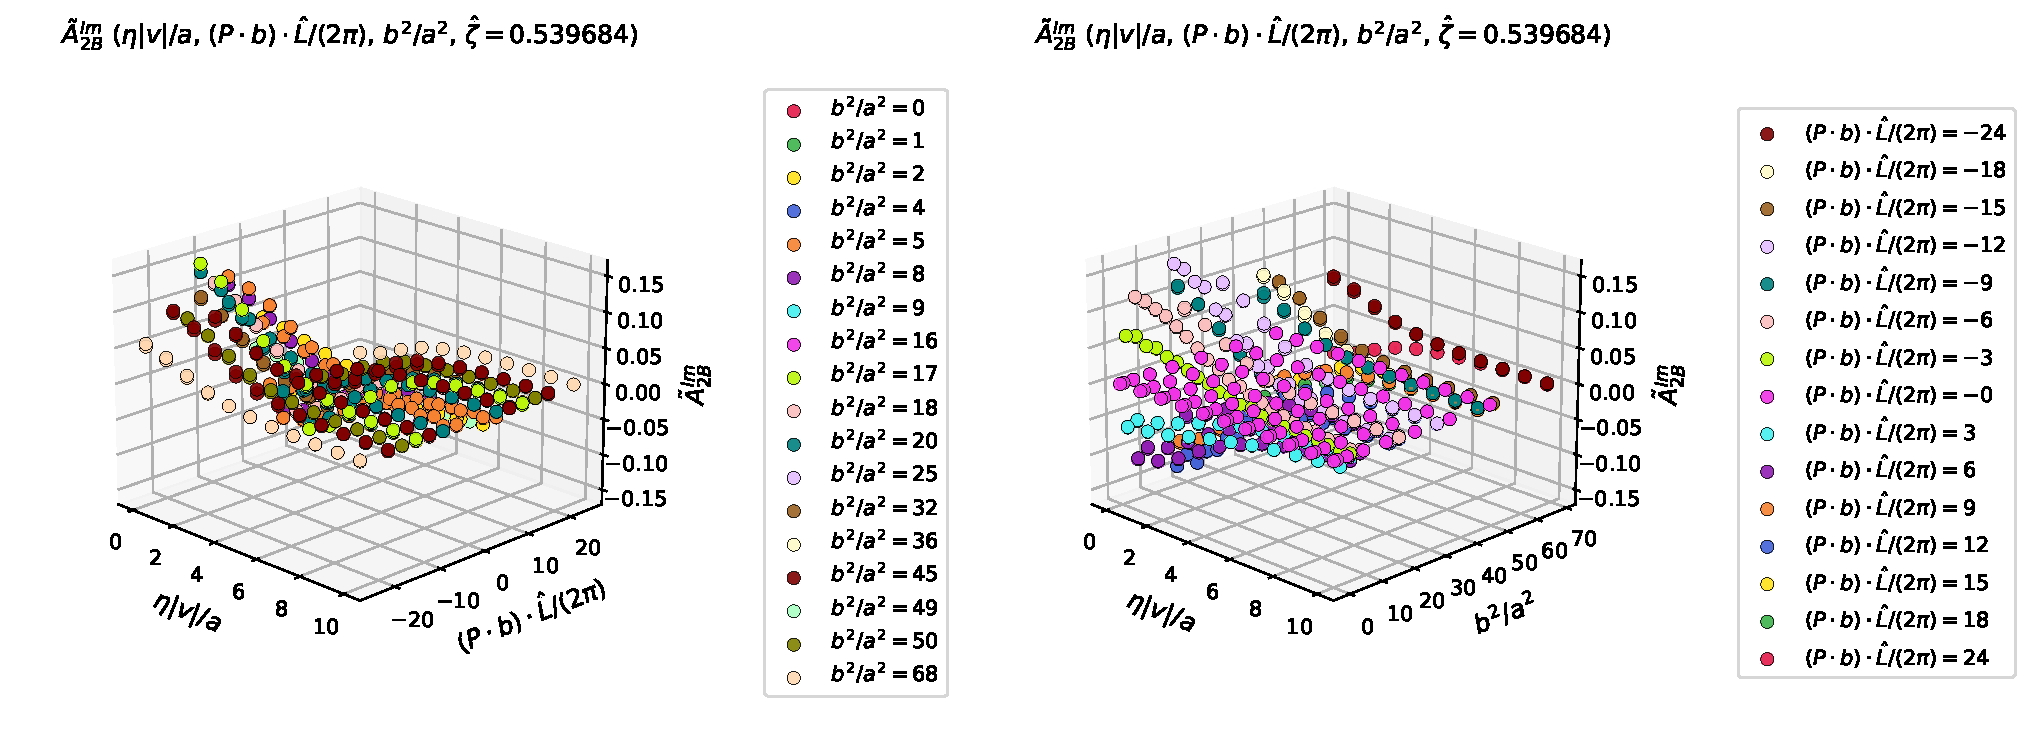
\includegraphics[width=0.98\linewidth,height=0.73\textheight,keepaspectratio]{ImA2B_Pb_bsq_PL-3_3D.pdf}\\[1mm]
{\small $\zetahat=0.539684$; $(\nu,s)$; staple-length dependence}
\figsrc{Thesis, Ch. 5: raw amplitude profiles; complete original panels.}
\end{frame}

\begin{frame}{$\tAmp_{12B}^{\mathrm{Re}}$ at $P_L=-3$: lattice coordinates}
\centering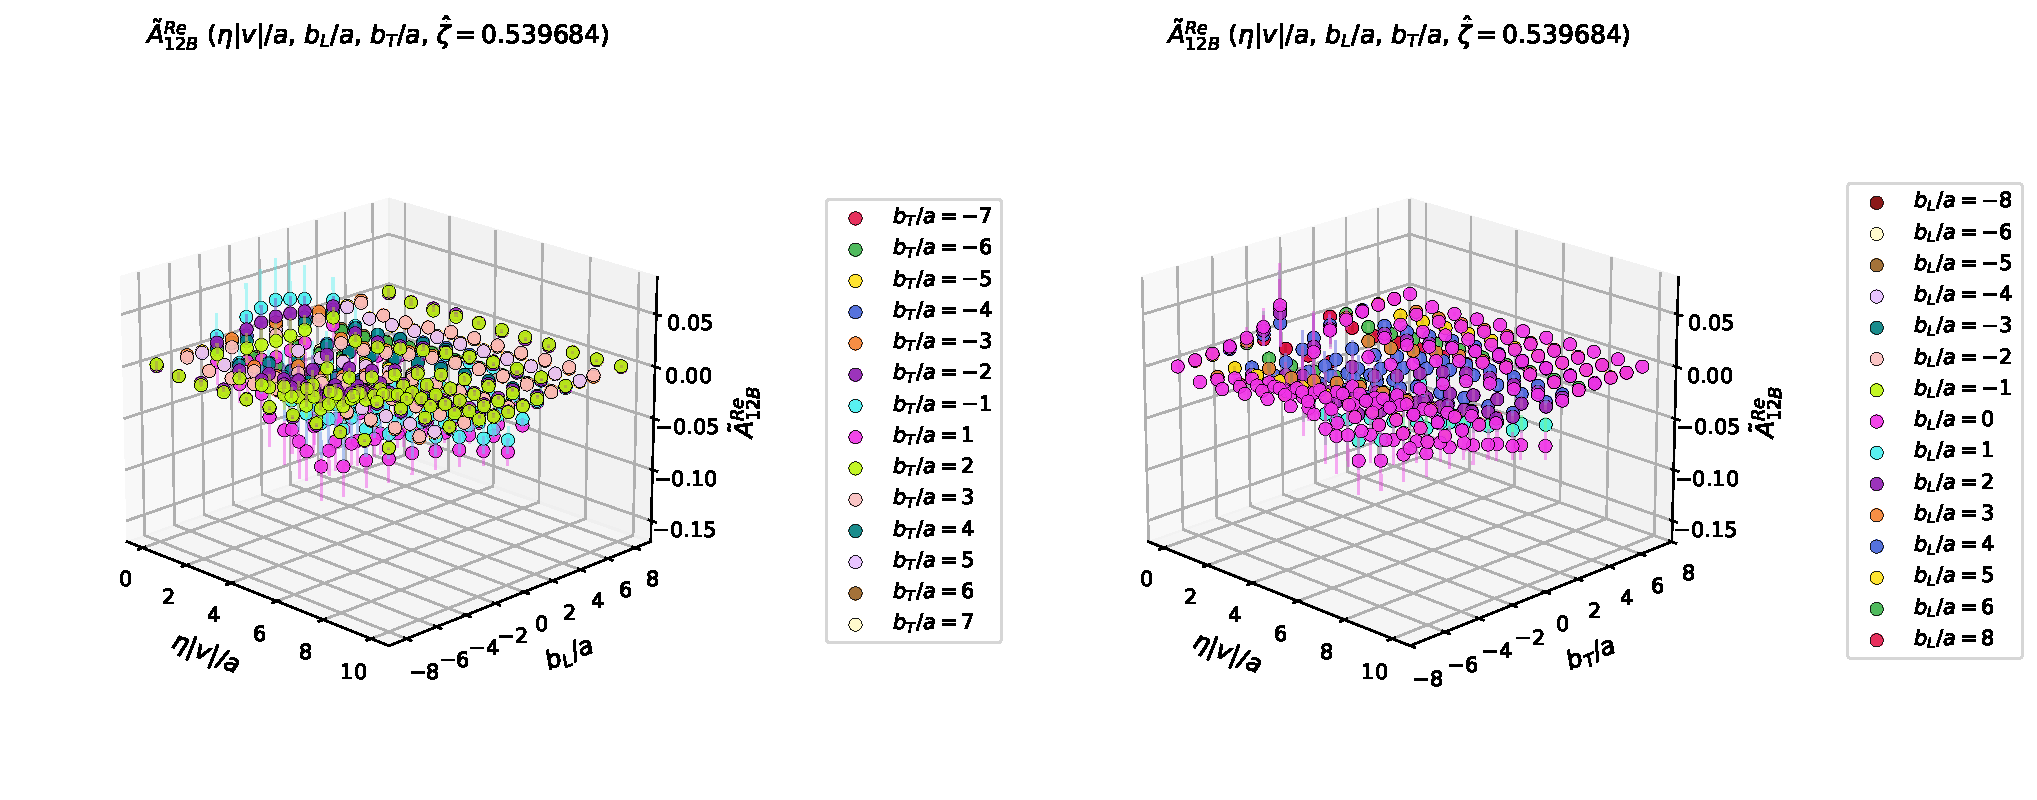
\includegraphics[width=0.98\linewidth,height=0.73\textheight,keepaspectratio]{ReA12B_PL-3_3D.pdf}\\[1mm]
{\small $\zetahat=0.539684$; $(b_L,b_T)$; staple-length dependence}
\figsrc{Thesis, Ch. 5: raw amplitude profiles; complete original panels.}
\end{frame}

\begin{frame}{$\tAmp_{12B}^{\mathrm{Re}}$ at $P_L=-3$: invariant coordinates}
\centering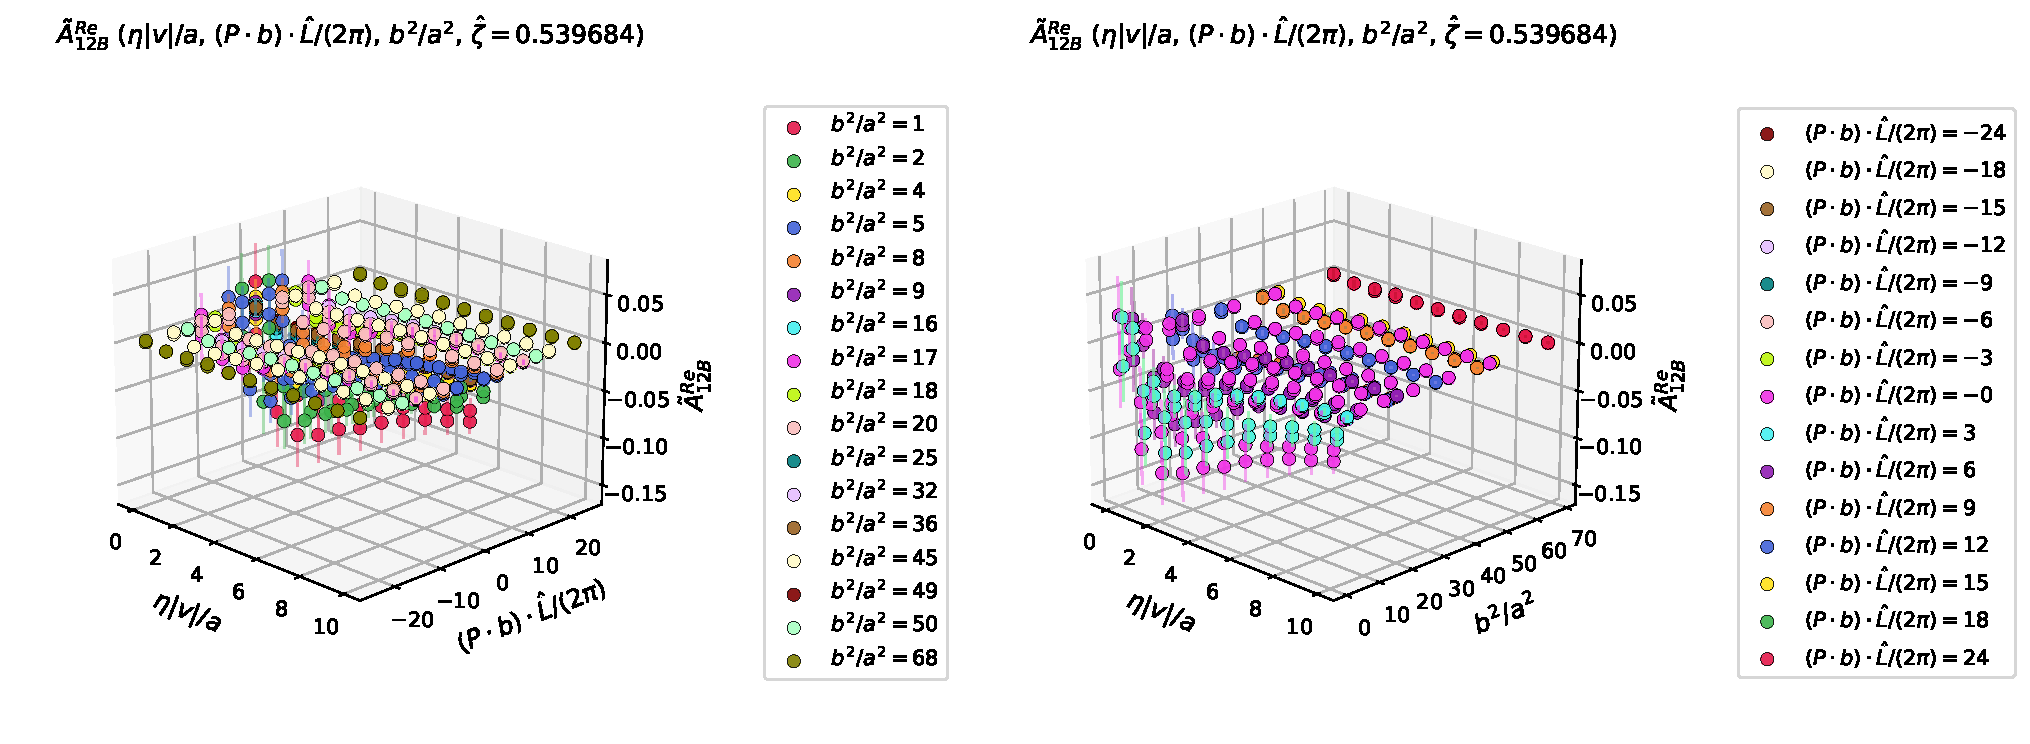
\includegraphics[width=0.98\linewidth,height=0.73\textheight,keepaspectratio]{ReA12B_Pb_bsq_PL-3_3D.pdf}\\[1mm]
{\small $\zetahat=0.539684$; $(\nu,s)$; staple-length dependence}
\figsrc{Thesis, Ch. 5: raw amplitude profiles; complete original panels.}
\end{frame}

\begin{frame}{$\tAmp_{12B}^{\mathrm{Im}}$ at $P_L=-3$: lattice coordinates}
\centering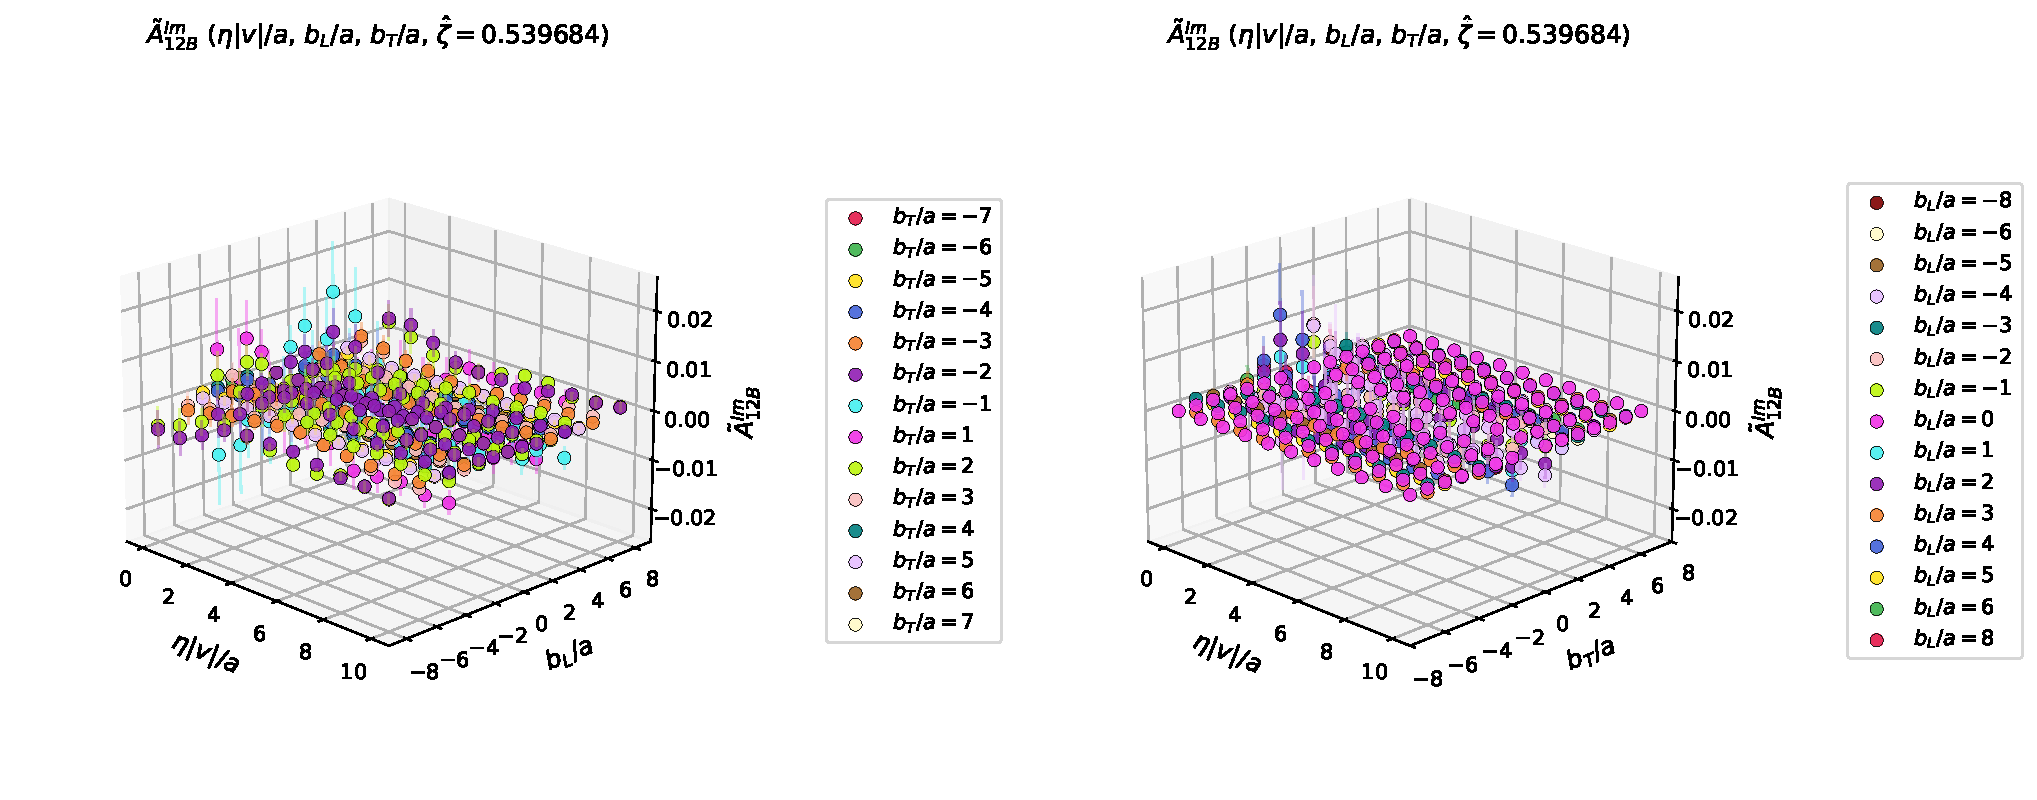
\includegraphics[width=0.98\linewidth,height=0.73\textheight,keepaspectratio]{ImA12B_PL-3_3D.pdf}\\[1mm]
{\small $\zetahat=0.539684$; $(b_L,b_T)$; staple-length dependence}
\figsrc{Thesis, Ch. 5: raw amplitude profiles; complete original panels.}
\end{frame}

\begin{frame}{$\tAmp_{12B}^{\mathrm{Im}}$ at $P_L=-3$: invariant coordinates}
\centering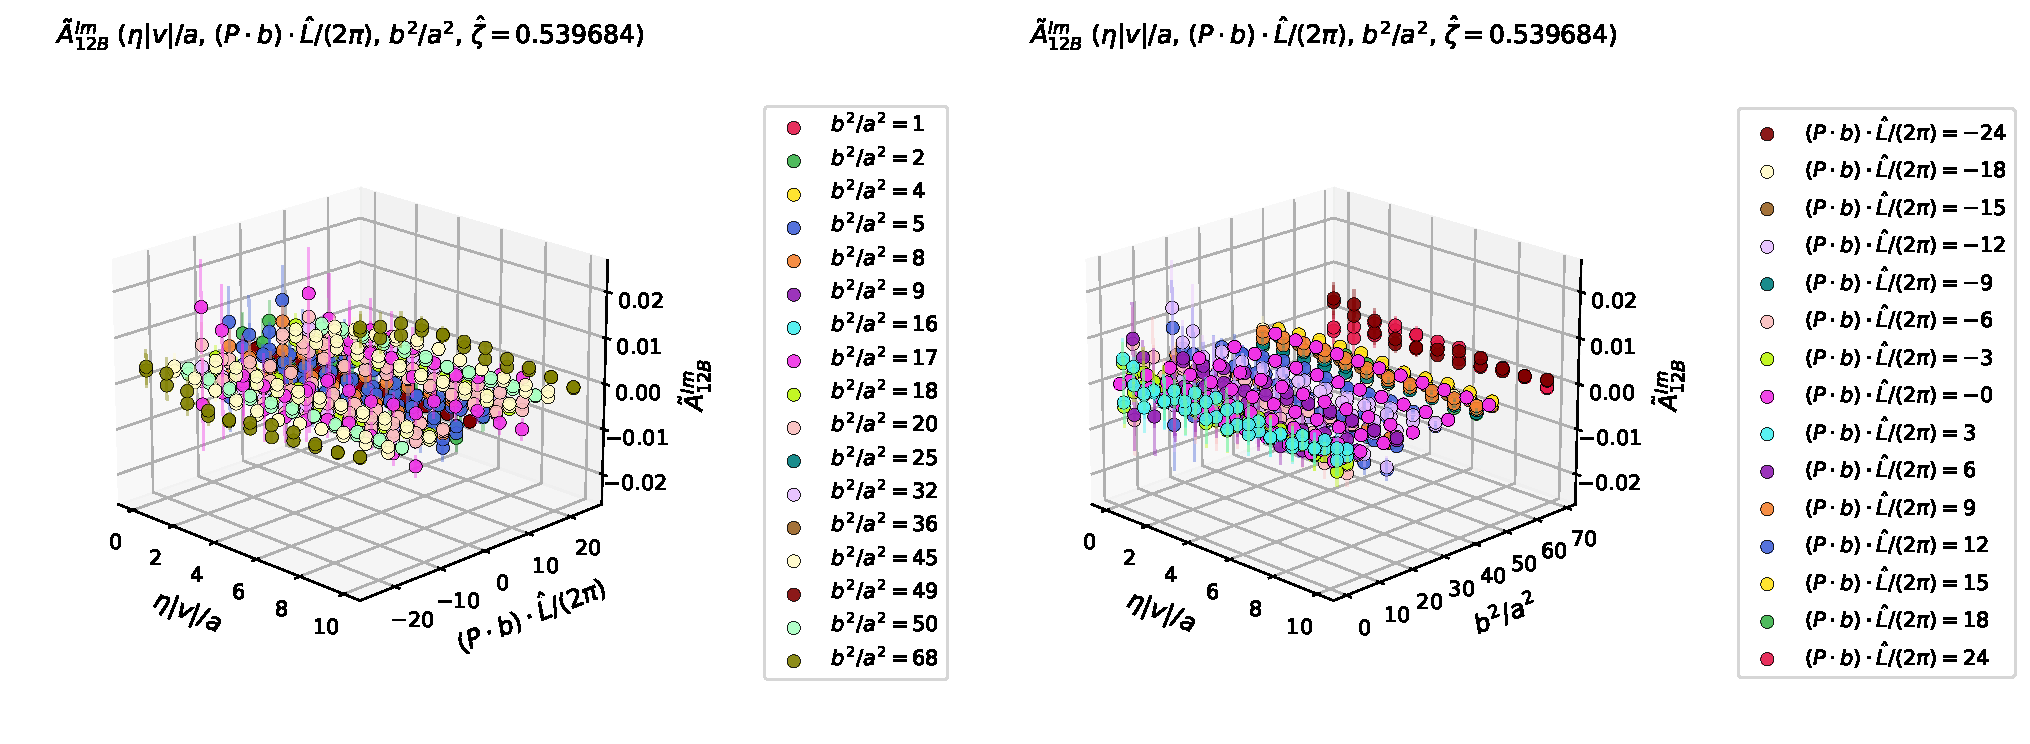
\includegraphics[width=0.98\linewidth,height=0.73\textheight,keepaspectratio]{ImA12B_Pb_bsq_PL-3_3D.pdf}\\[1mm]
{\small $\zetahat=0.539684$; $(\nu,s)$; staple-length dependence}
\figsrc{Thesis, Ch. 5: raw amplitude profiles; complete original panels.}
\end{frame}

\begin{frame}{$\tAmp_{2B}^{\mathrm{Re}}$ at $P_L=-3$: lattice coordinates}
\centering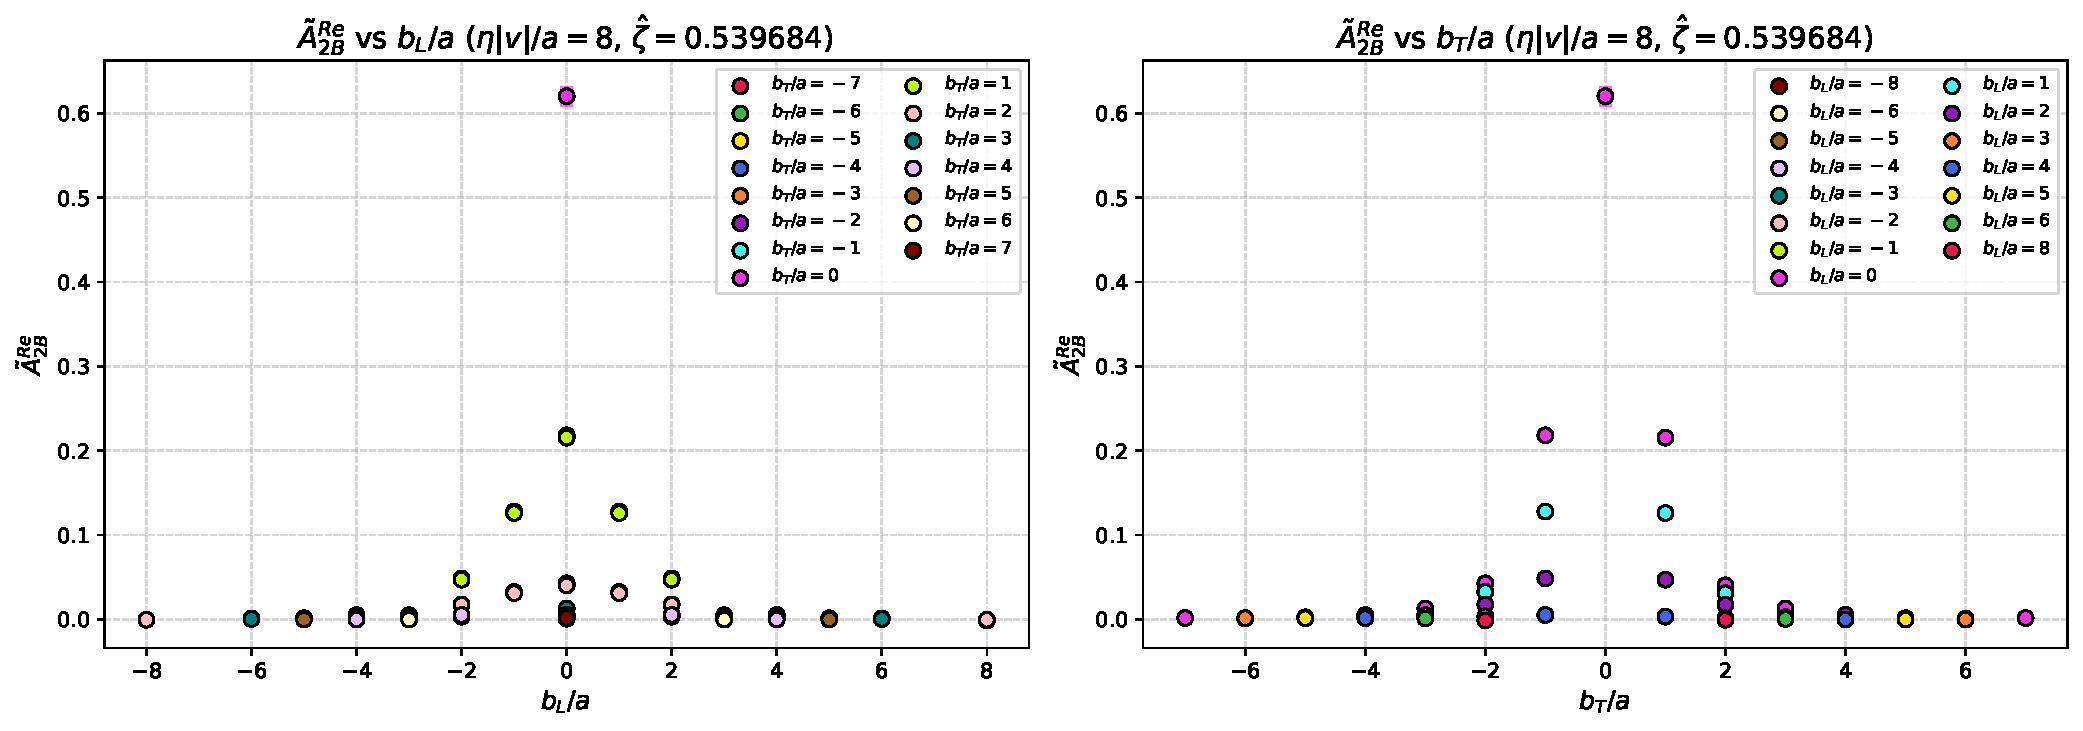
\includegraphics[width=0.98\linewidth,height=0.73\textheight,keepaspectratio]{ReA2B_eta8_PL-3_2D.pdf}\\[1mm]
{\small $\zetahat=0.539684$; $(b_L,b_T)$; $\eta|v|/a=8$ slices}
\figsrc{Thesis, Ch. 5: raw amplitude profiles; complete original panels.}
\end{frame}

\begin{frame}{$\tAmp_{2B}^{\mathrm{Re}}$ at $P_L=-3$: invariant coordinates}
\centering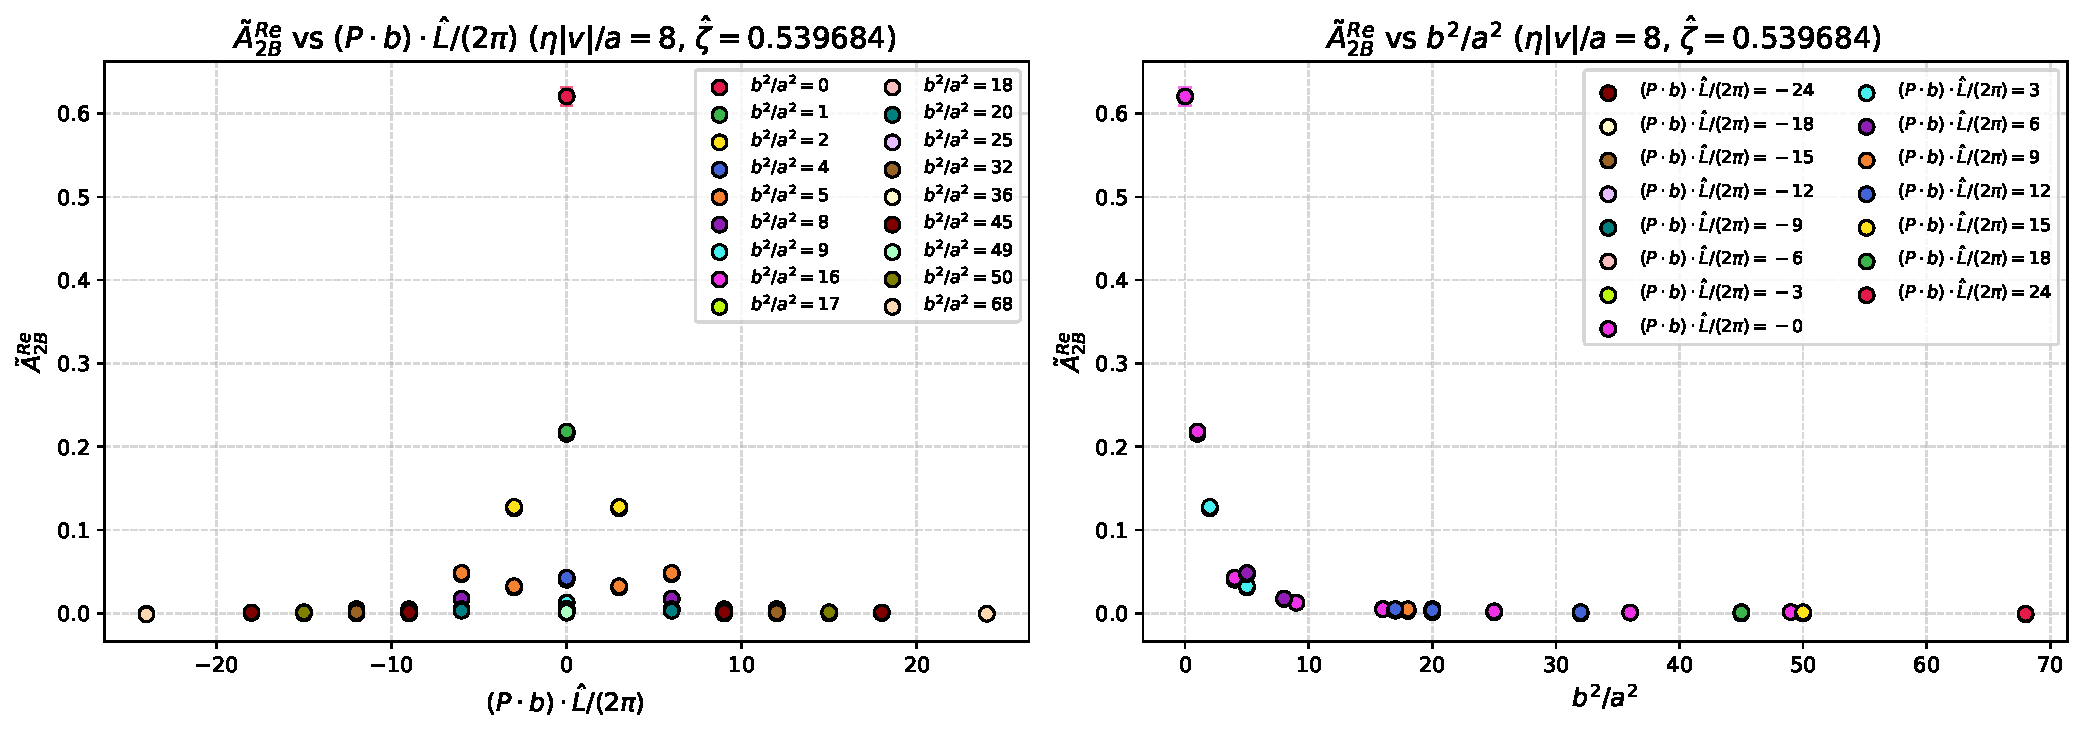
\includegraphics[width=0.98\linewidth,height=0.73\textheight,keepaspectratio]{ReA2B_Pb_bsq_eta8_PL-3_2D.pdf}\\[1mm]
{\small $\zetahat=0.539684$; $(\nu,s)$; $\eta|v|/a=8$ slices}
\figsrc{Thesis, Ch. 5: raw amplitude profiles; complete original panels.}
\end{frame}

\begin{frame}{$\tAmp_{2B}^{\mathrm{Im}}$ at $P_L=-3$: lattice coordinates}
\centering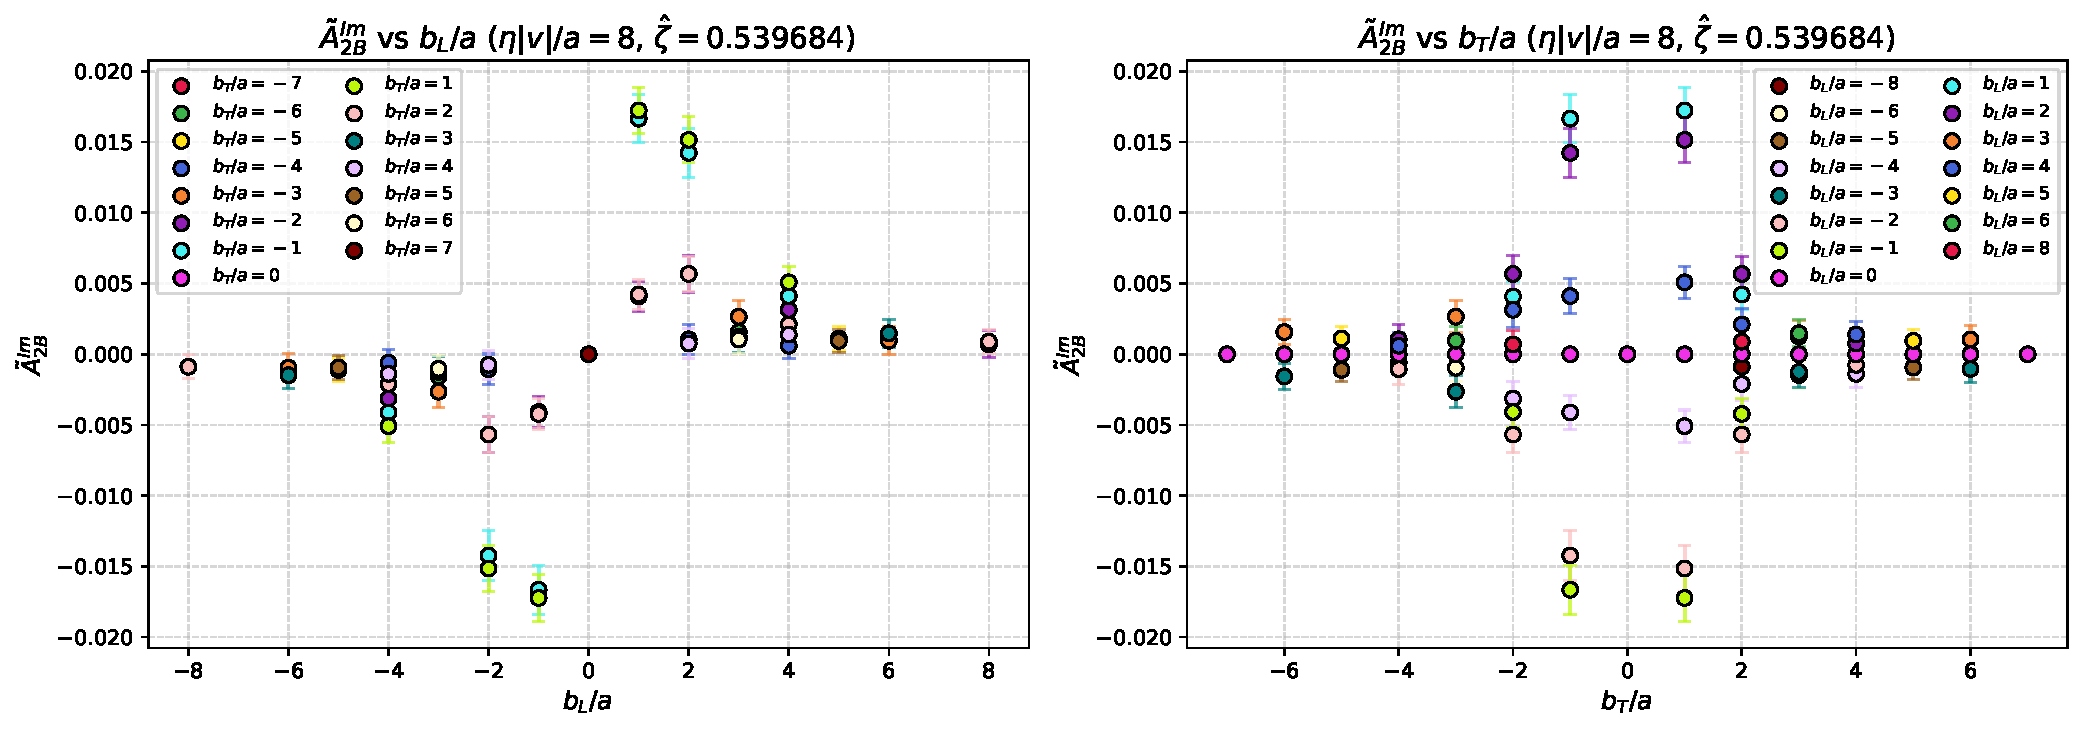
\includegraphics[width=0.98\linewidth,height=0.73\textheight,keepaspectratio]{ImA2B_eta8_PL-3_2D.pdf}\\[1mm]
{\small $\zetahat=0.539684$; $(b_L,b_T)$; $\eta|v|/a=8$ slices}
\figsrc{Thesis, Ch. 5: raw amplitude profiles; complete original panels.}
\end{frame}

\begin{frame}{$\tAmp_{2B}^{\mathrm{Im}}$ at $P_L=-3$: invariant coordinates}
\centering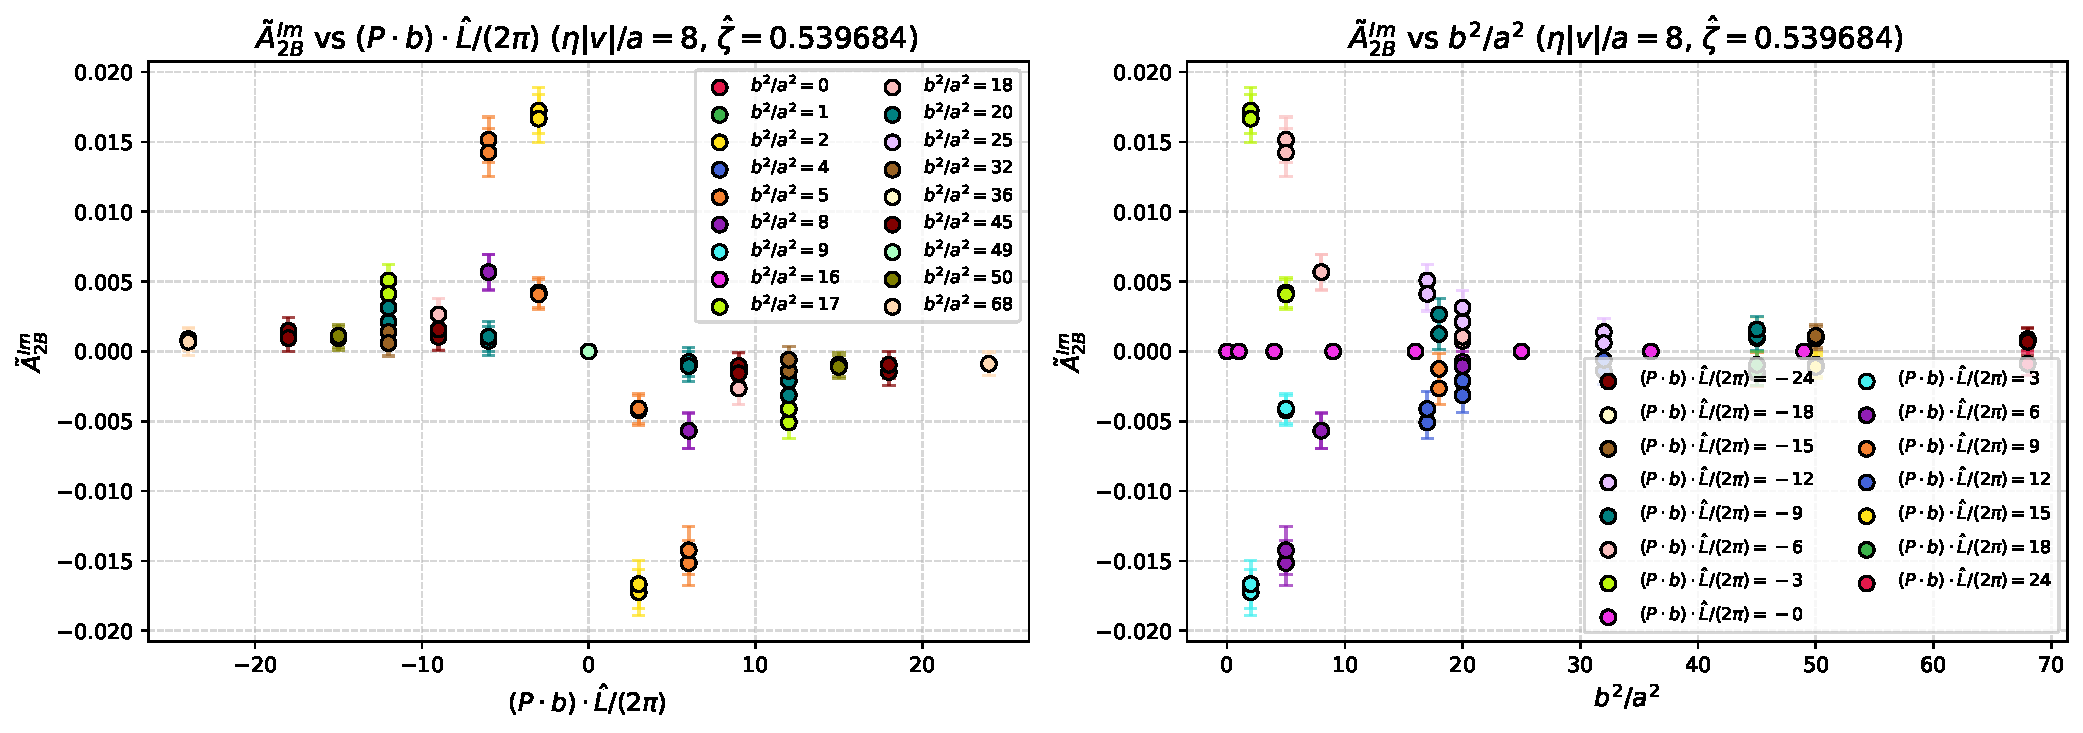
\includegraphics[width=0.98\linewidth,height=0.73\textheight,keepaspectratio]{ImA2B_Pb_bsq_eta8_PL-3_2D.pdf}\\[1mm]
{\small $\zetahat=0.539684$; $(\nu,s)$; $\eta|v|/a=8$ slices}
\figsrc{Thesis, Ch. 5: raw amplitude profiles; complete original panels.}
\end{frame}

\begin{frame}{$\tAmp_{12B}^{\mathrm{Re}}$ at $P_L=-3$: lattice coordinates}
\centering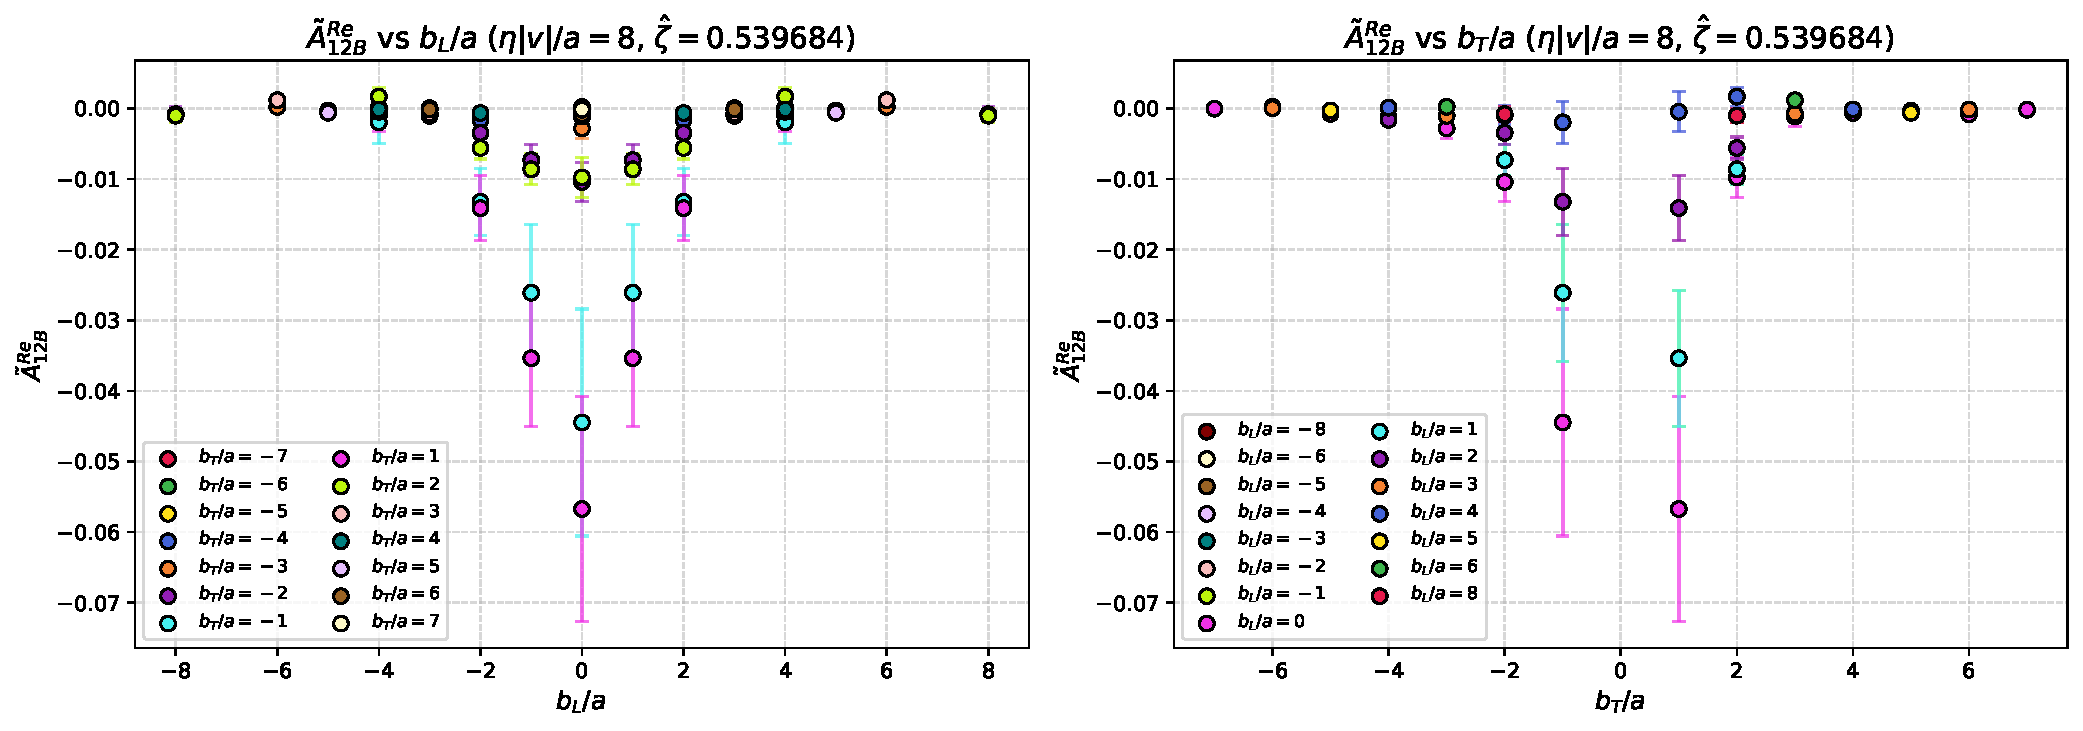
\includegraphics[width=0.98\linewidth,height=0.73\textheight,keepaspectratio]{ReA12B_eta8_PL-3_2D.pdf}\\[1mm]
{\small $\zetahat=0.539684$; $(b_L,b_T)$; $\eta|v|/a=8$ slices}
\figsrc{Thesis, Ch. 5: raw amplitude profiles; complete original panels.}
\end{frame}

\begin{frame}{$\tAmp_{12B}^{\mathrm{Re}}$ at $P_L=-3$: invariant coordinates}
\centering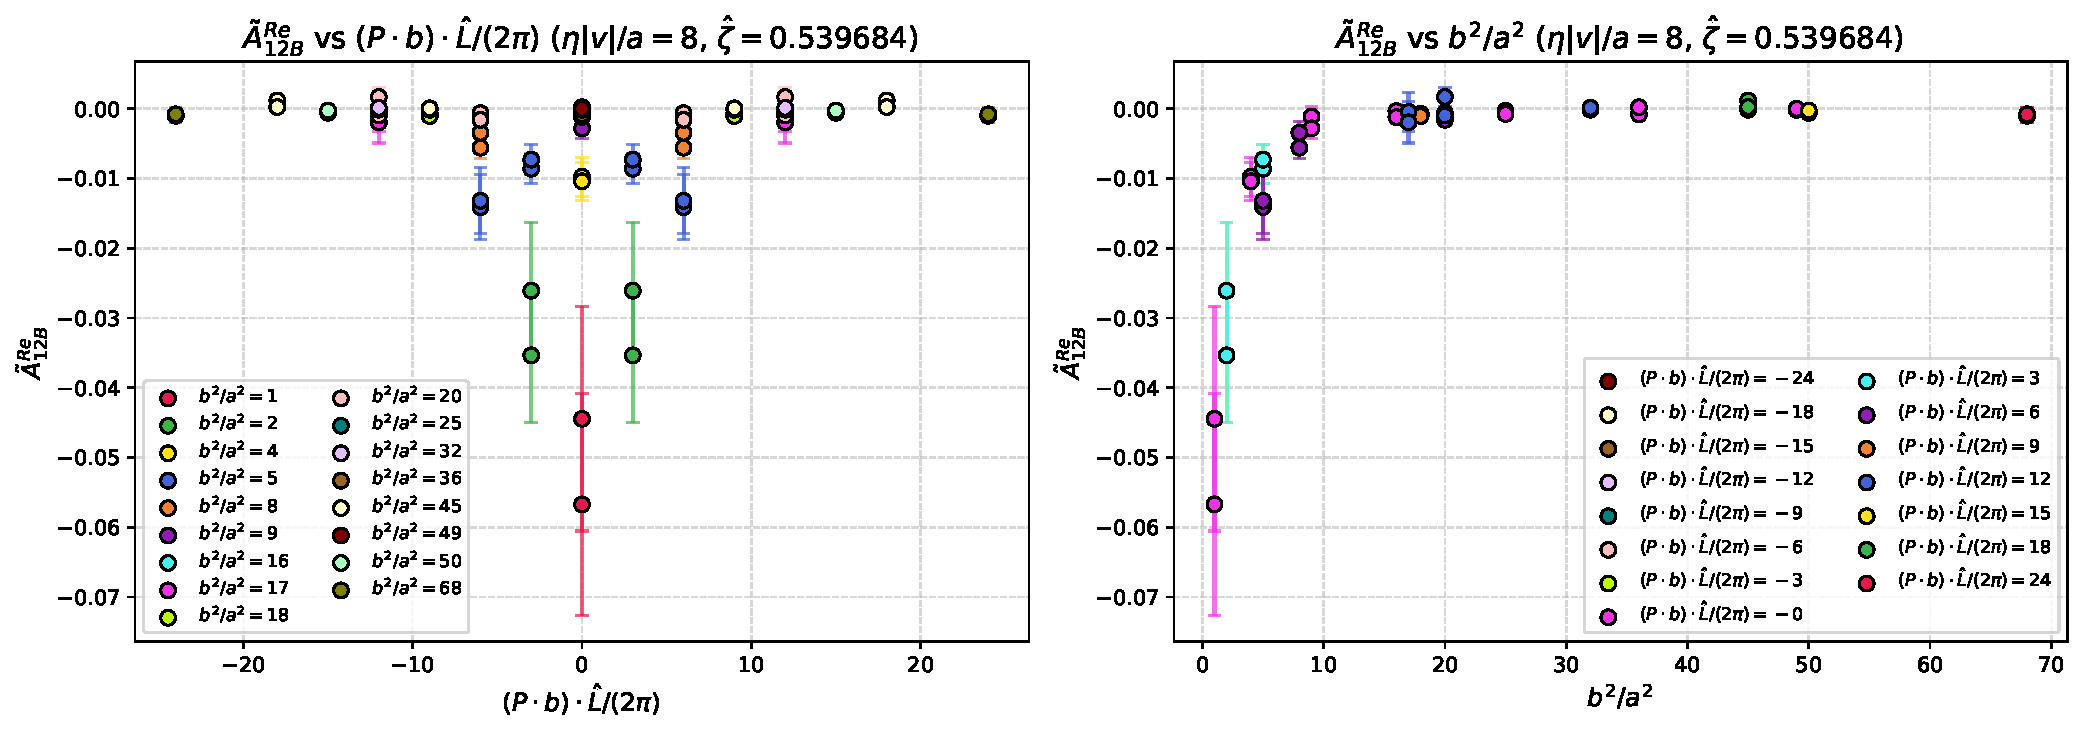
\includegraphics[width=0.98\linewidth,height=0.73\textheight,keepaspectratio]{ReA12B_Pb_bsq_eta8_PL-3_2D.pdf}\\[1mm]
{\small $\zetahat=0.539684$; $(\nu,s)$; $\eta|v|/a=8$ slices}
\figsrc{Thesis, Ch. 5: raw amplitude profiles; complete original panels.}
\end{frame}

\begin{frame}{$\tAmp_{12B}^{\mathrm{Im}}$ at $P_L=-3$: lattice coordinates}
\centering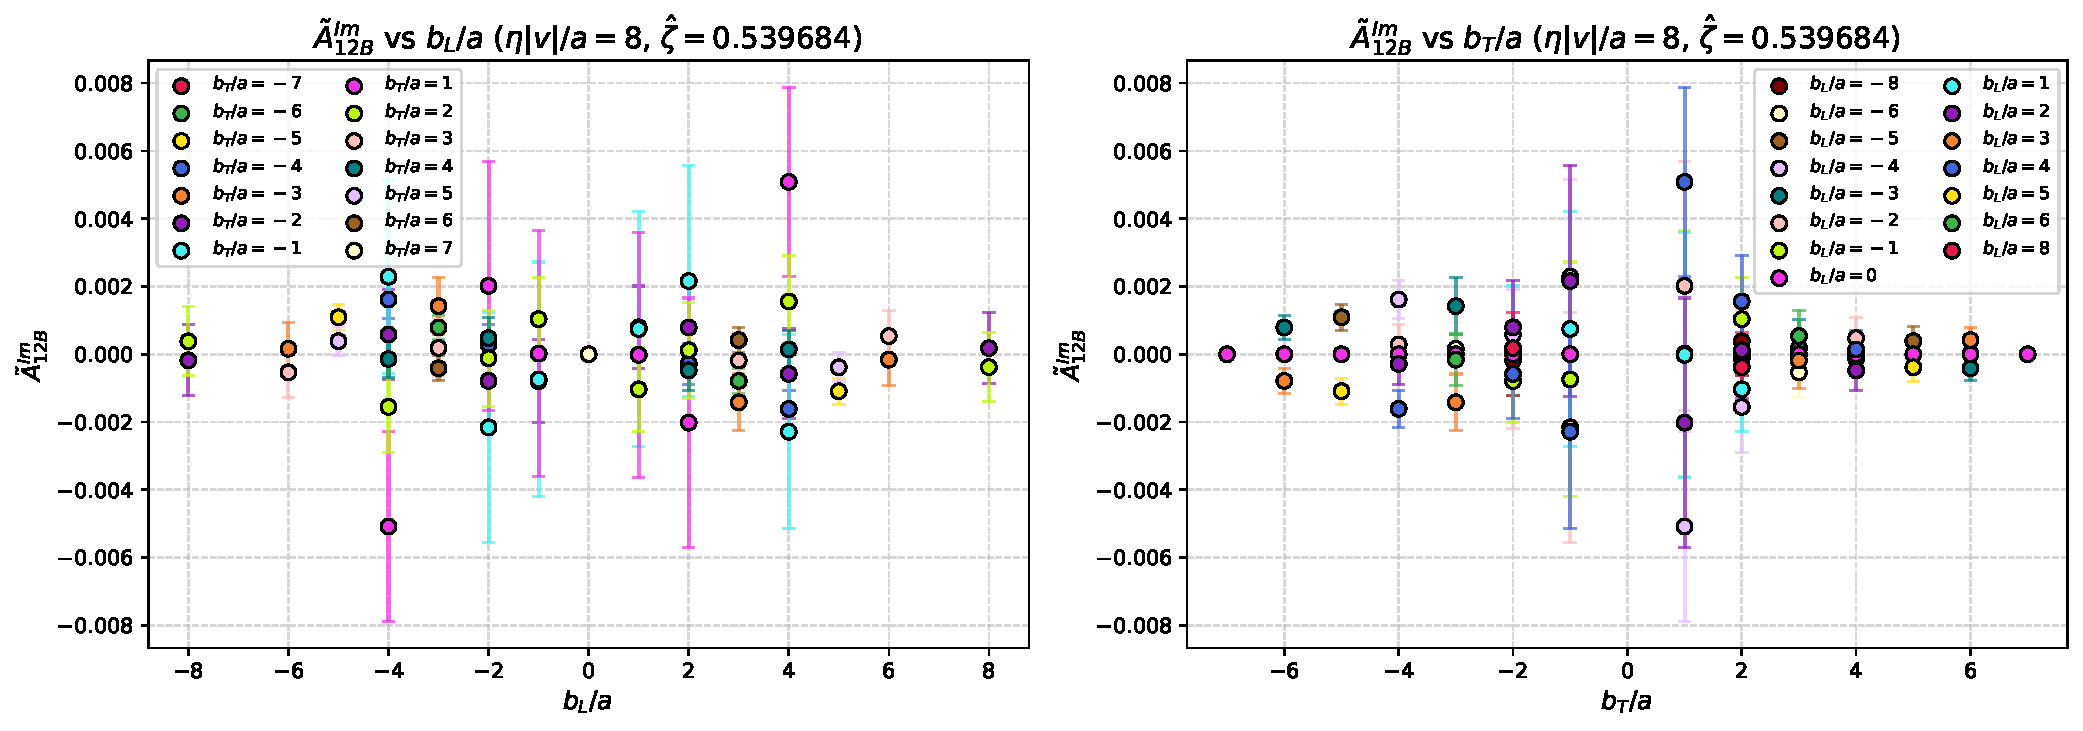
\includegraphics[width=0.98\linewidth,height=0.73\textheight,keepaspectratio]{ImA12B_eta8_PL-3_2D.pdf}\\[1mm]
{\small $\zetahat=0.539684$; $(b_L,b_T)$; $\eta|v|/a=8$ slices}
\figsrc{Thesis, Ch. 5: raw amplitude profiles; complete original panels.}
\end{frame}

\begin{frame}{$\tAmp_{12B}^{\mathrm{Im}}$ at $P_L=-3$: invariant coordinates}
\centering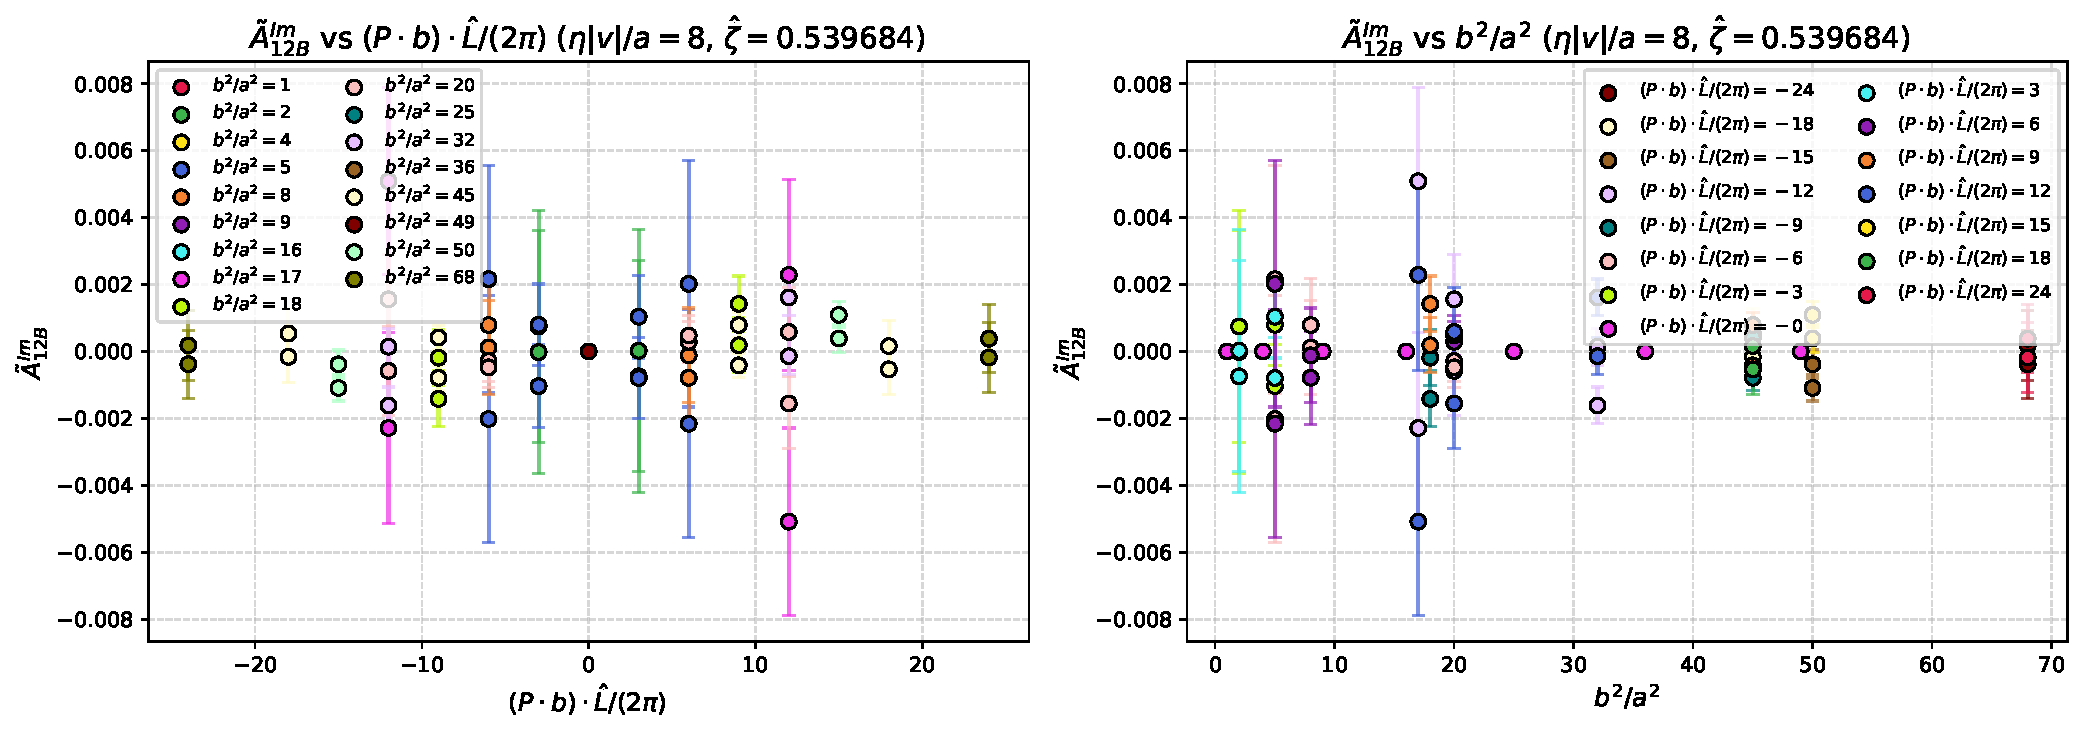
\includegraphics[width=0.98\linewidth,height=0.73\textheight,keepaspectratio]{ImA12B_Pb_bsq_eta8_PL-3_2D.pdf}\\[1mm]
{\small $\zetahat=0.539684$; $(\nu,s)$; $\eta|v|/a=8$ slices}
\figsrc{Thesis, Ch. 5: raw amplitude profiles; complete original panels.}
\end{frame}

\begin{frame}{$\tAmp_{2B}^{\mathrm{Re}}$ at $P_L=-4$: lattice coordinates}
\centering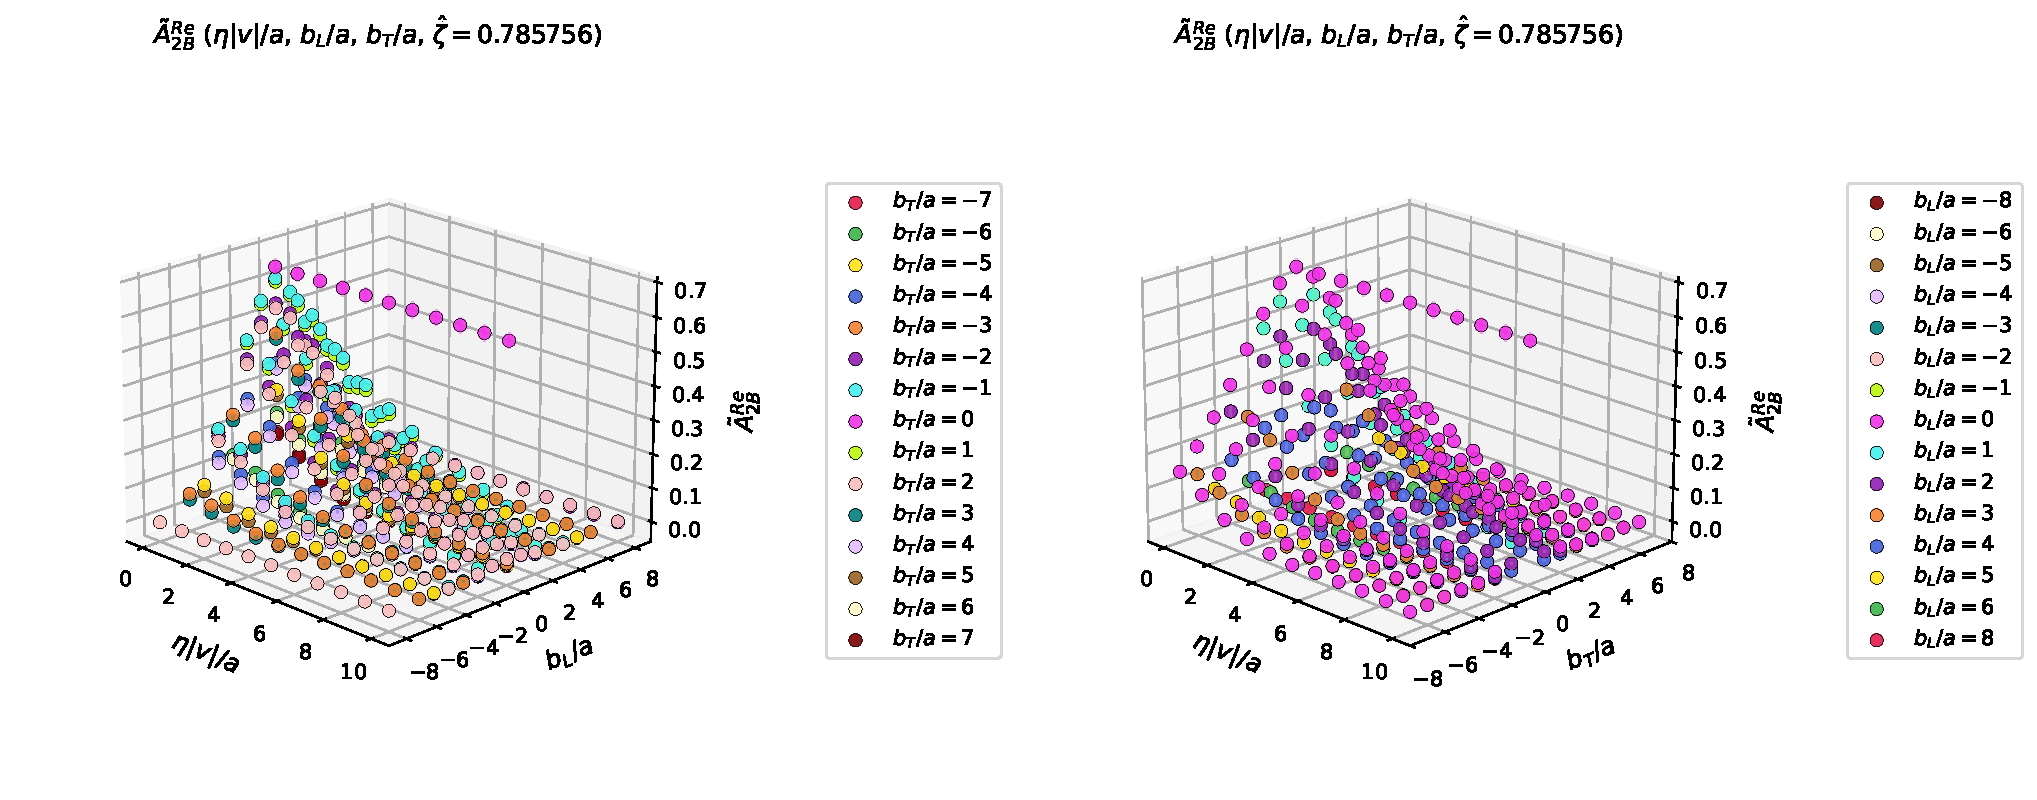
\includegraphics[width=0.98\linewidth,height=0.73\textheight,keepaspectratio]{ReA2B_PL-4_3D.pdf}\\[1mm]
{\small $\zetahat=0.785756$; $(b_L,b_T)$; staple-length dependence}
\figsrc{Thesis, Ch. 5: raw amplitude profiles; complete original panels.}
\end{frame}

\begin{frame}{$\tAmp_{2B}^{\mathrm{Re}}$ at $P_L=-4$: invariant coordinates}
\centering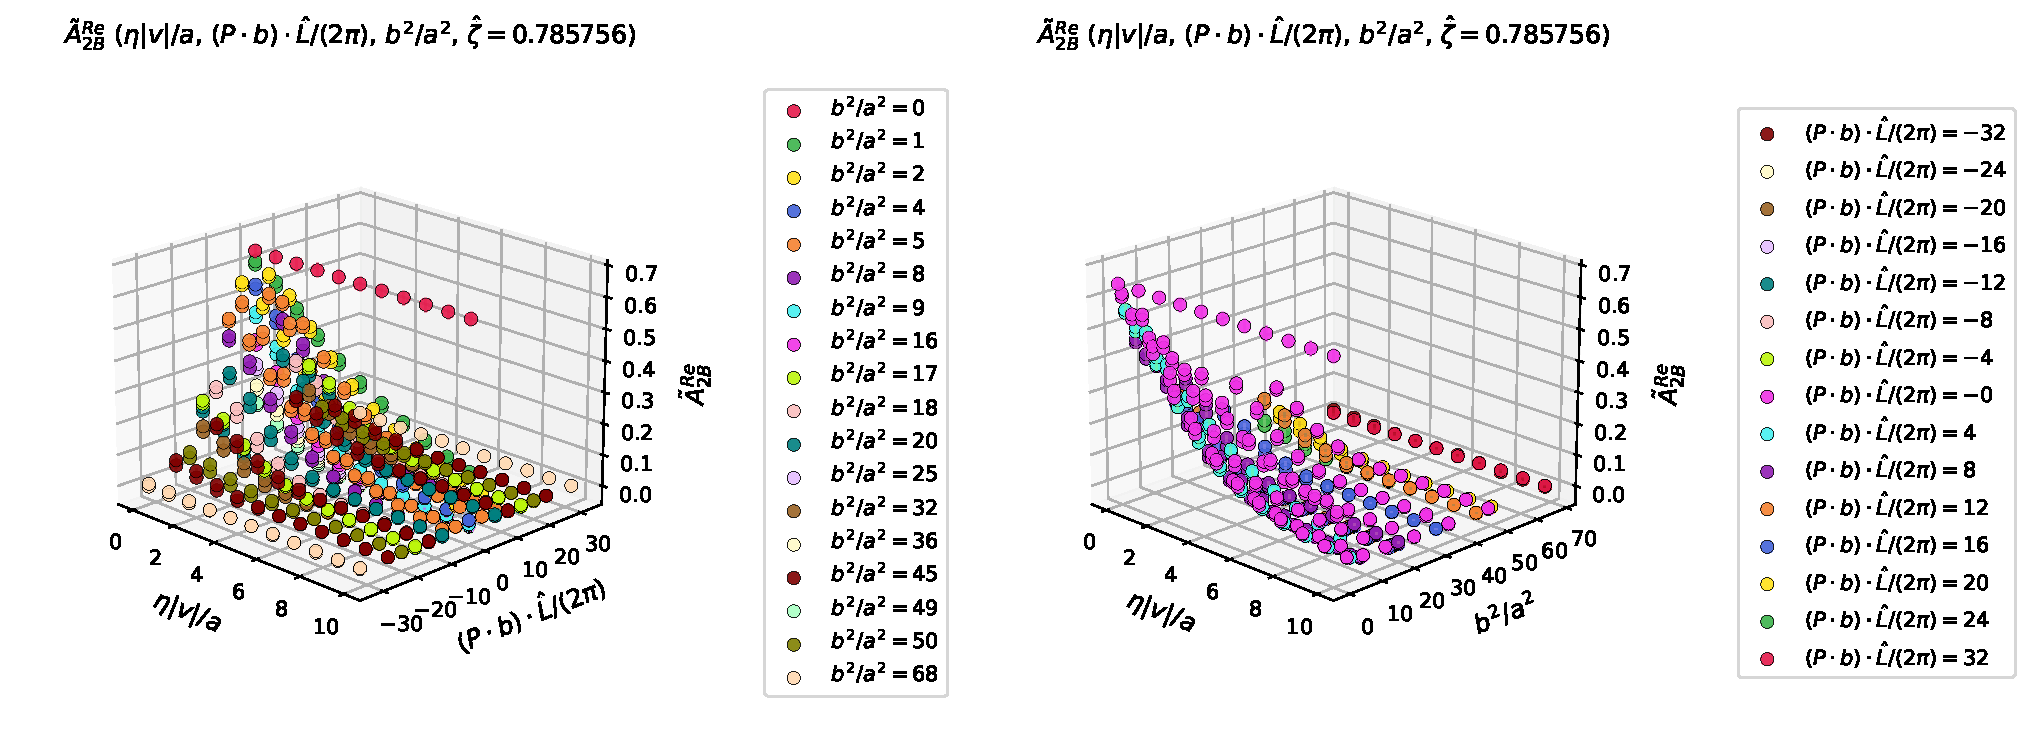
\includegraphics[width=0.98\linewidth,height=0.73\textheight,keepaspectratio]{ReA2B_Pb_bsq_PL-4_3D.pdf}\\[1mm]
{\small $\zetahat=0.785756$; $(\nu,s)$; staple-length dependence}
\figsrc{Thesis, Ch. 5: raw amplitude profiles; complete original panels.}
\end{frame}

\begin{frame}{$\tAmp_{2B}^{\mathrm{Im}}$ at $P_L=-4$: lattice coordinates}
\centering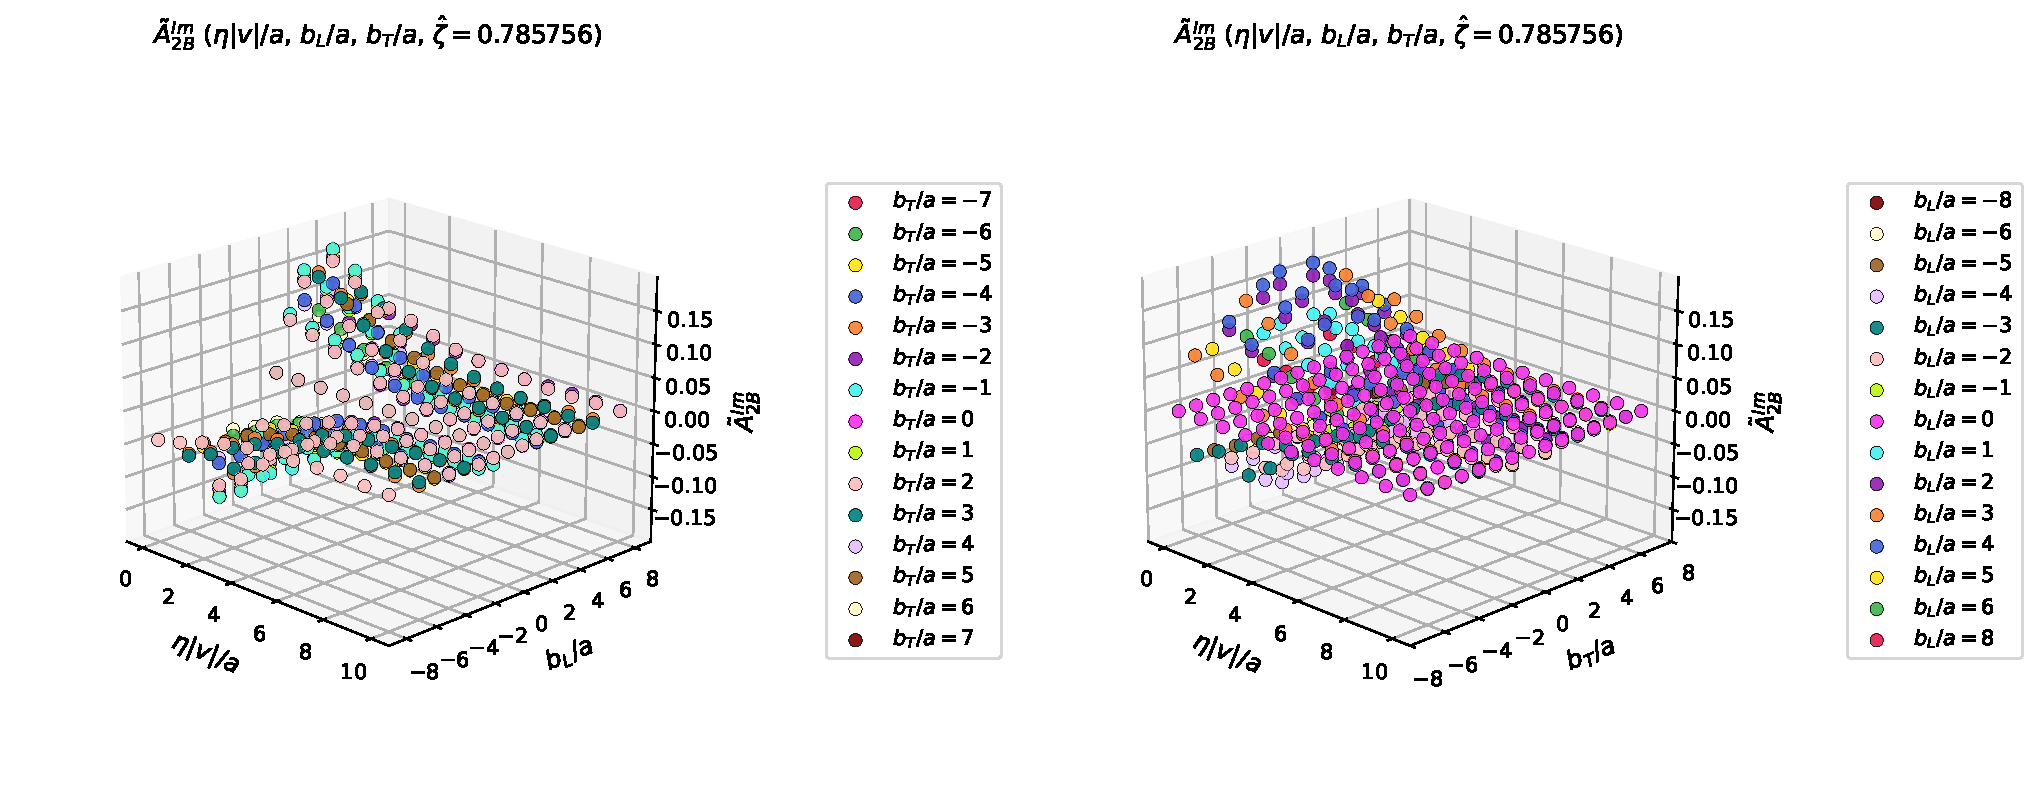
\includegraphics[width=0.98\linewidth,height=0.73\textheight,keepaspectratio]{ImA2B_PL-4_3D.pdf}\\[1mm]
{\small $\zetahat=0.785756$; $(b_L,b_T)$; staple-length dependence}
\figsrc{Thesis, Ch. 5: raw amplitude profiles; complete original panels.}
\end{frame}

\begin{frame}{$\tAmp_{2B}^{\mathrm{Im}}$ at $P_L=-4$: invariant coordinates}
\centering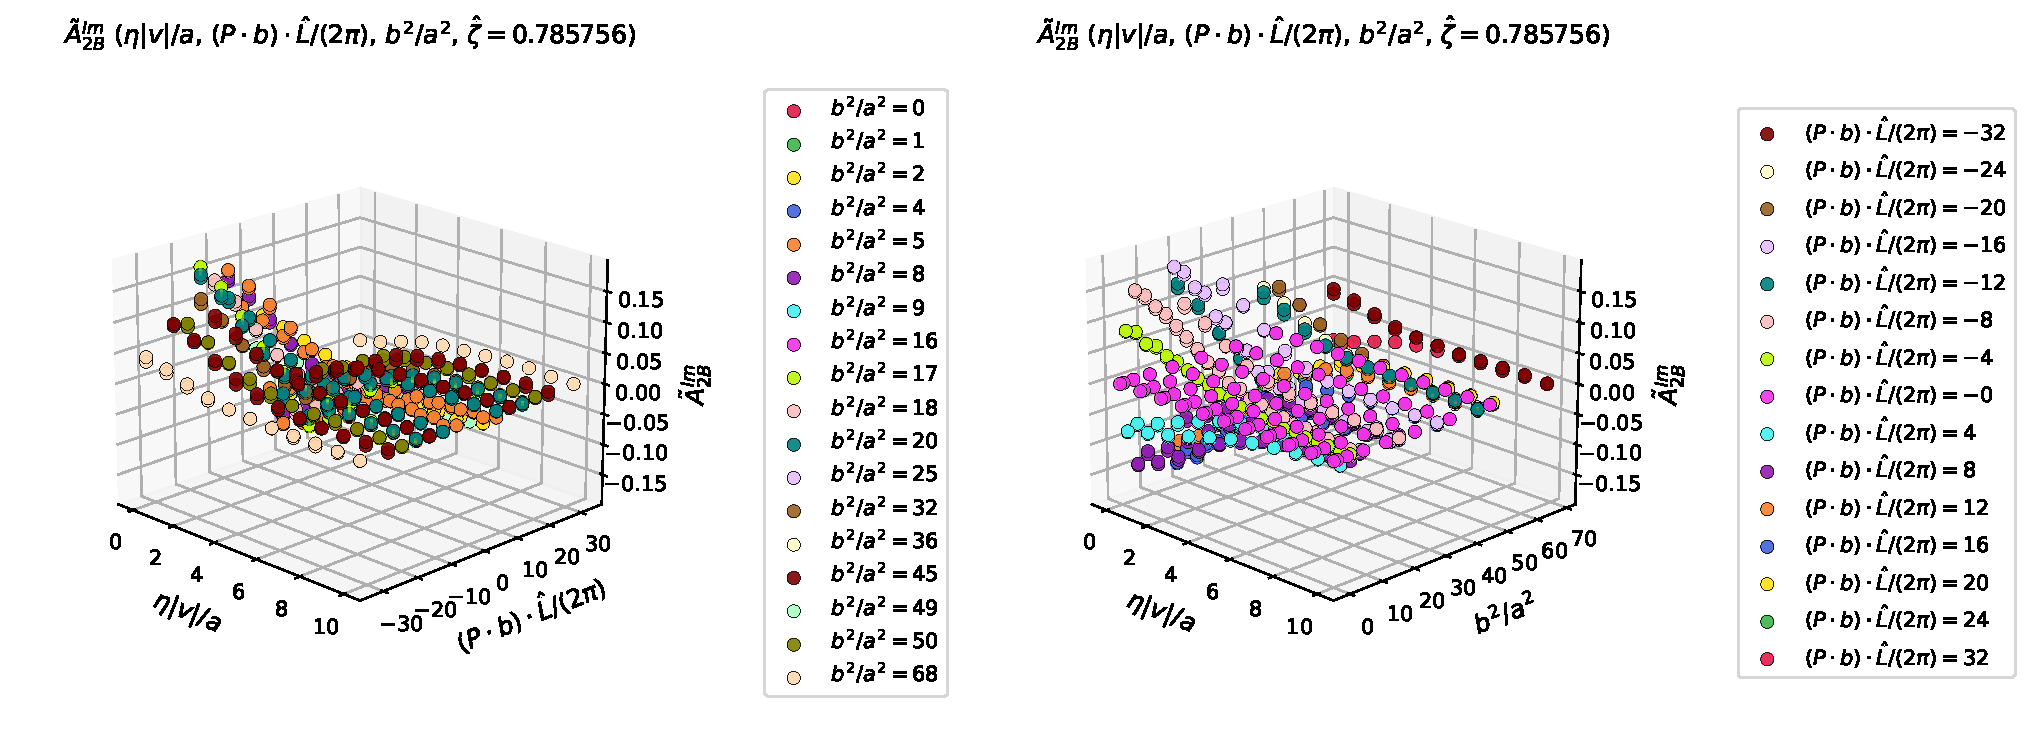
\includegraphics[width=0.98\linewidth,height=0.73\textheight,keepaspectratio]{ImA2B_Pb_bsq_PL-4_3D.pdf}\\[1mm]
{\small $\zetahat=0.785756$; $(\nu,s)$; staple-length dependence}
\figsrc{Thesis, Ch. 5: raw amplitude profiles; complete original panels.}
\end{frame}

\begin{frame}{$\tAmp_{12B}^{\mathrm{Re}}$ at $P_L=-4$: lattice coordinates}
\centering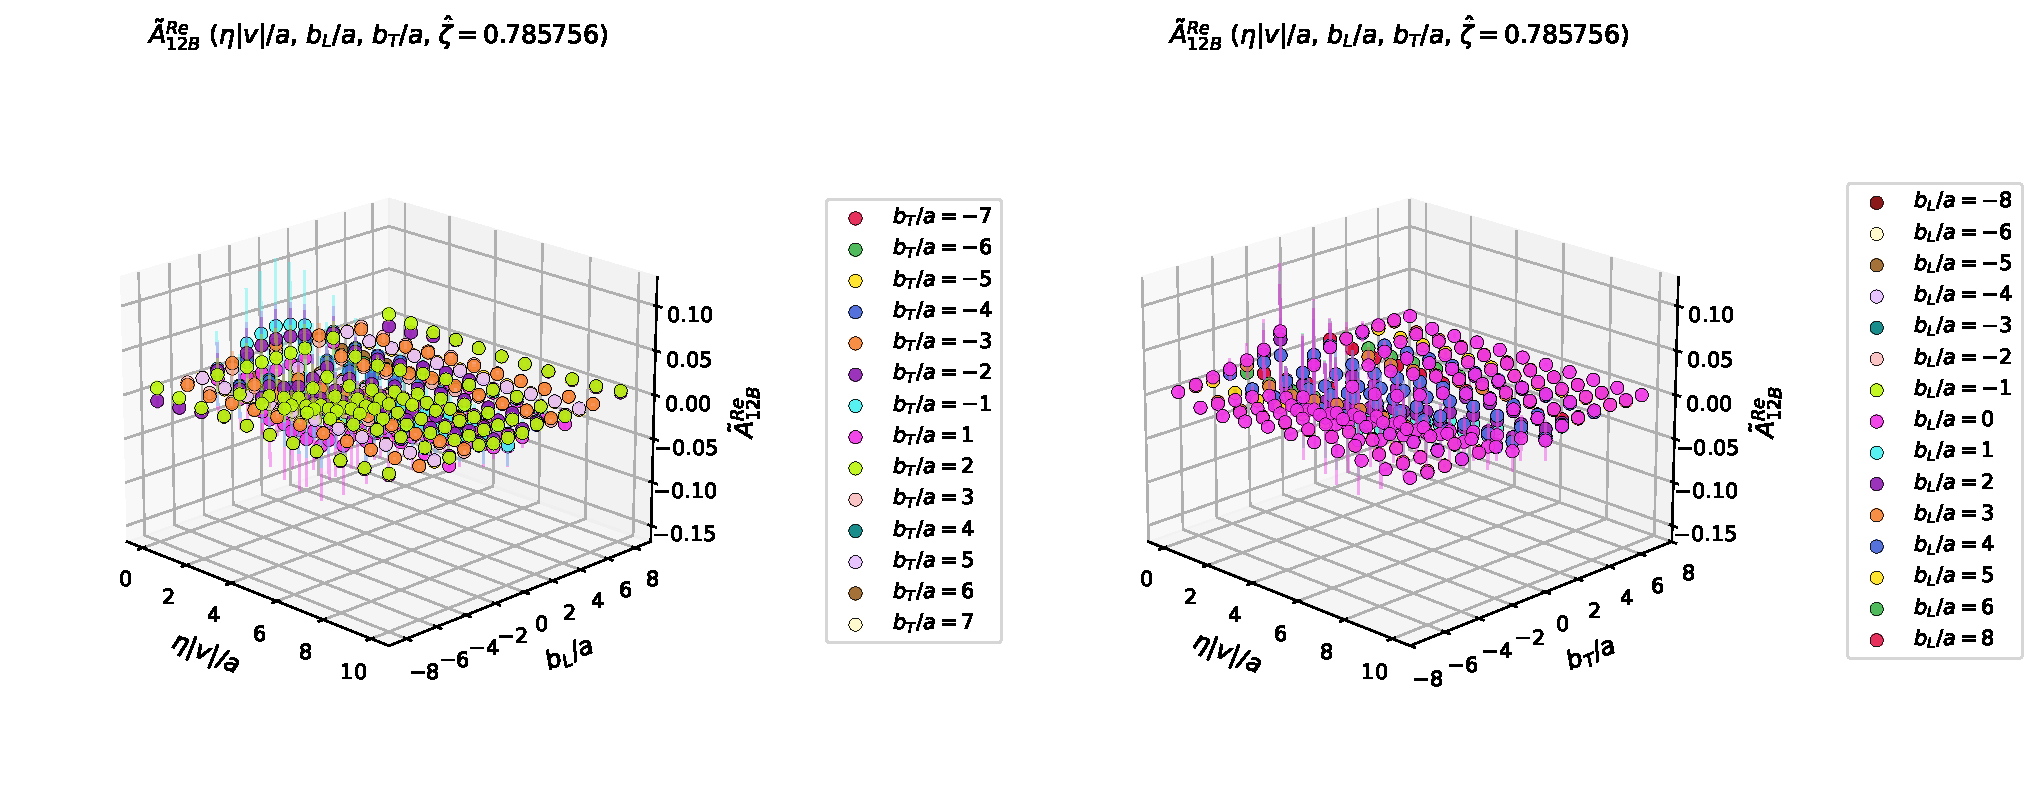
\includegraphics[width=0.98\linewidth,height=0.73\textheight,keepaspectratio]{ReA12B_PL-4_3D.pdf}\\[1mm]
{\small $\zetahat=0.785756$; $(b_L,b_T)$; staple-length dependence}
\figsrc{Thesis, Ch. 5: raw amplitude profiles; complete original panels.}
\end{frame}

\begin{frame}{$\tAmp_{12B}^{\mathrm{Re}}$ at $P_L=-4$: invariant coordinates}
\centering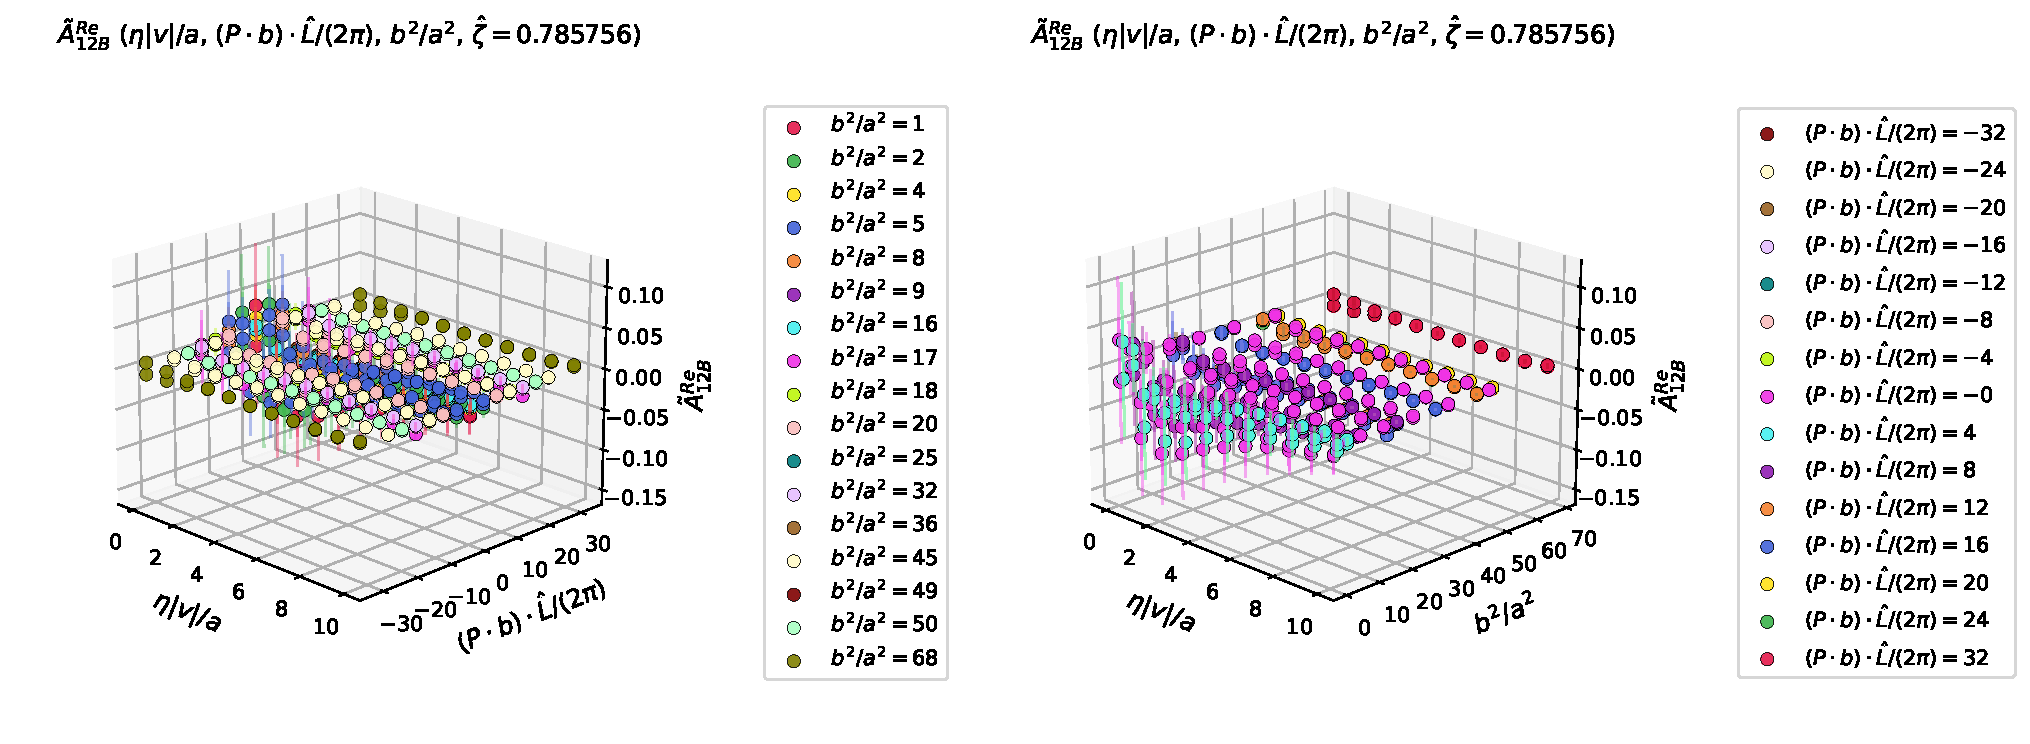
\includegraphics[width=0.98\linewidth,height=0.73\textheight,keepaspectratio]{ReA12B_Pb_bsq_PL-4_3D.pdf}\\[1mm]
{\small $\zetahat=0.785756$; $(\nu,s)$; staple-length dependence}
\figsrc{Thesis, Ch. 5: raw amplitude profiles; complete original panels.}
\end{frame}

\begin{frame}{$\tAmp_{12B}^{\mathrm{Im}}$ at $P_L=-4$: lattice coordinates}
\centering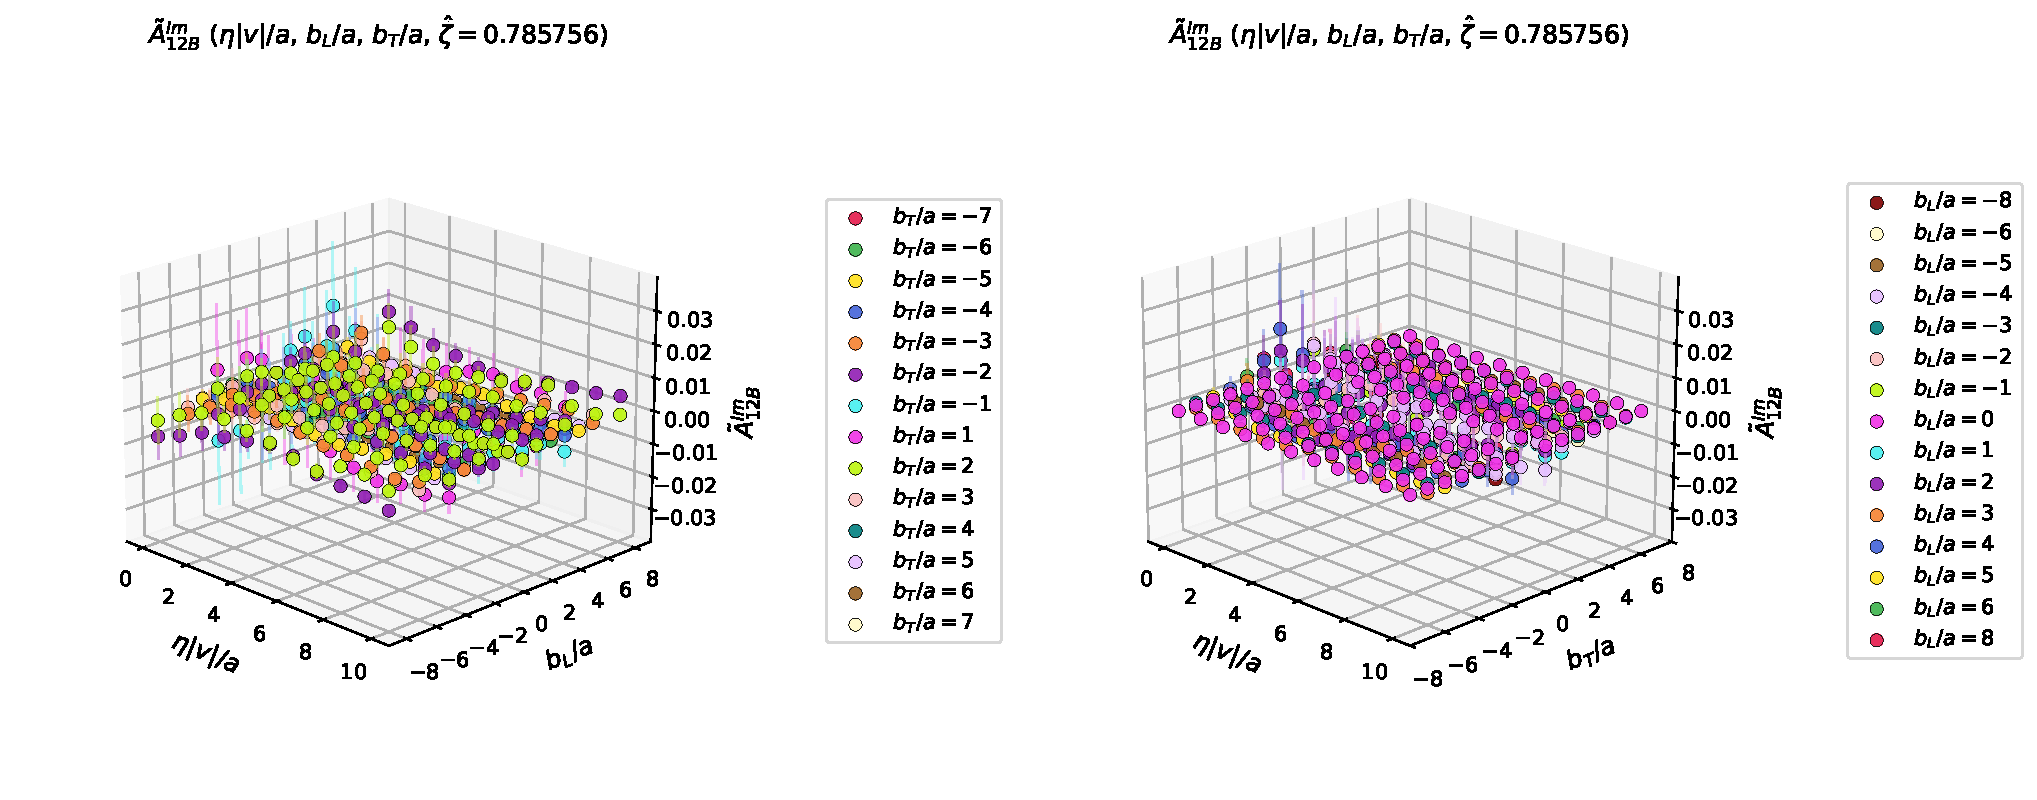
\includegraphics[width=0.98\linewidth,height=0.73\textheight,keepaspectratio]{ImA12B_PL-4_3D.pdf}\\[1mm]
{\small $\zetahat=0.785756$; $(b_L,b_T)$; staple-length dependence}
\figsrc{Thesis, Ch. 5: raw amplitude profiles; complete original panels.}
\end{frame}

\begin{frame}{$\tAmp_{12B}^{\mathrm{Im}}$ at $P_L=-4$: invariant coordinates}
\centering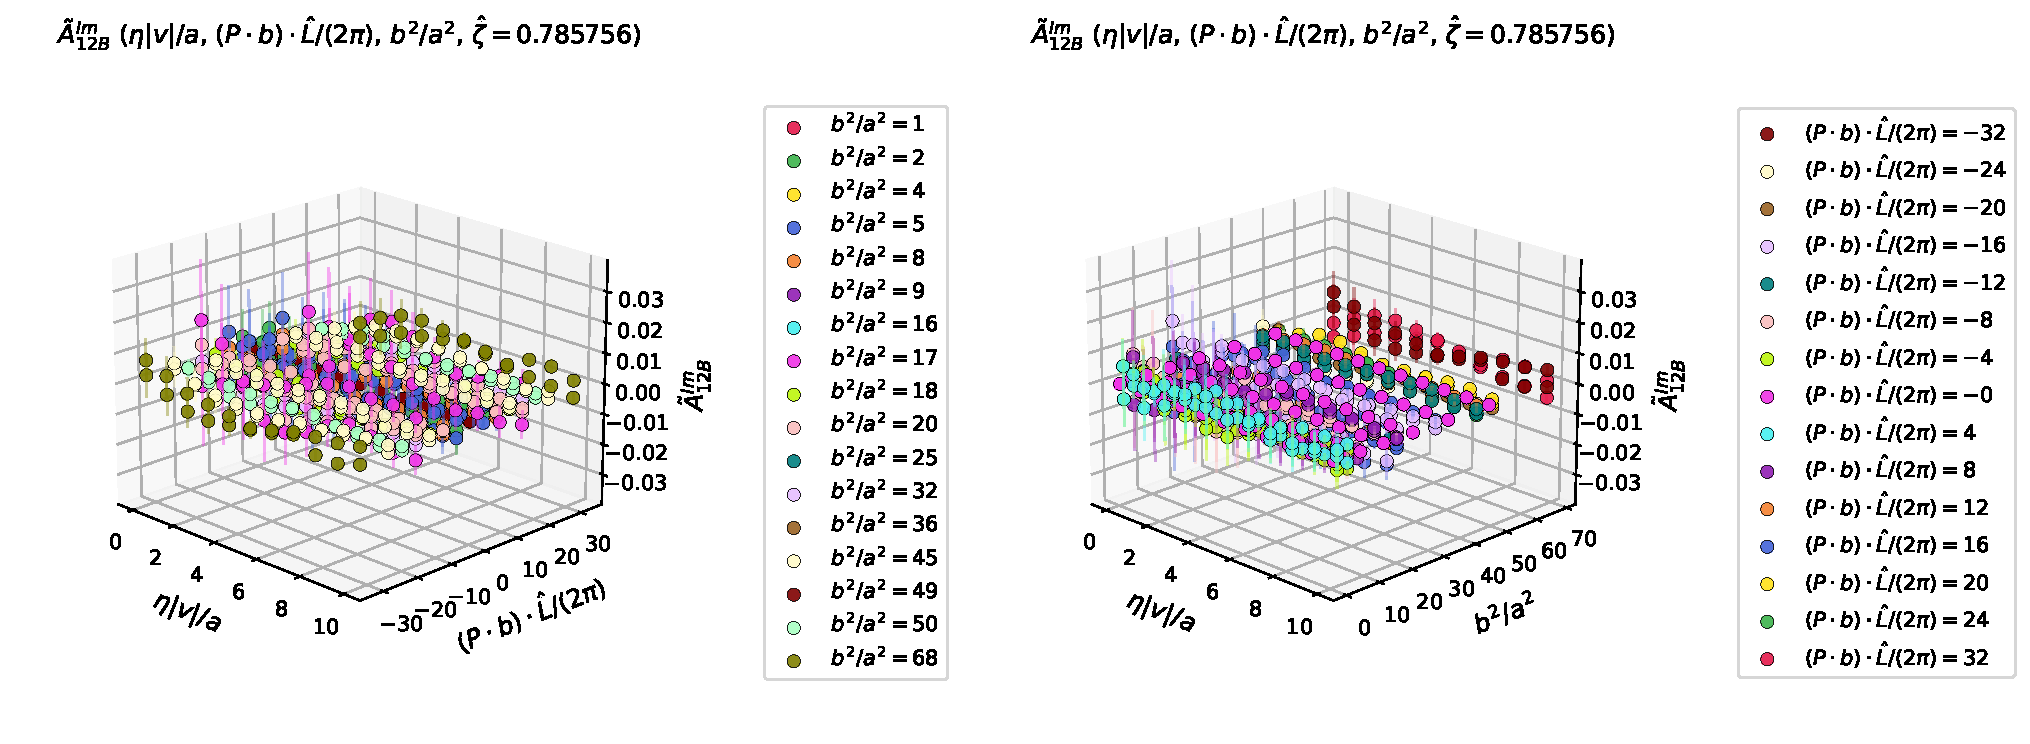
\includegraphics[width=0.98\linewidth,height=0.73\textheight,keepaspectratio]{ImA12B_Pb_bsq_PL-4_3D.pdf}\\[1mm]
{\small $\zetahat=0.785756$; $(\nu,s)$; staple-length dependence}
\figsrc{Thesis, Ch. 5: raw amplitude profiles; complete original panels.}
\end{frame}

\begin{frame}{$\tAmp_{2B}^{\mathrm{Re}}$ at $P_L=-4$: lattice coordinates}
\centering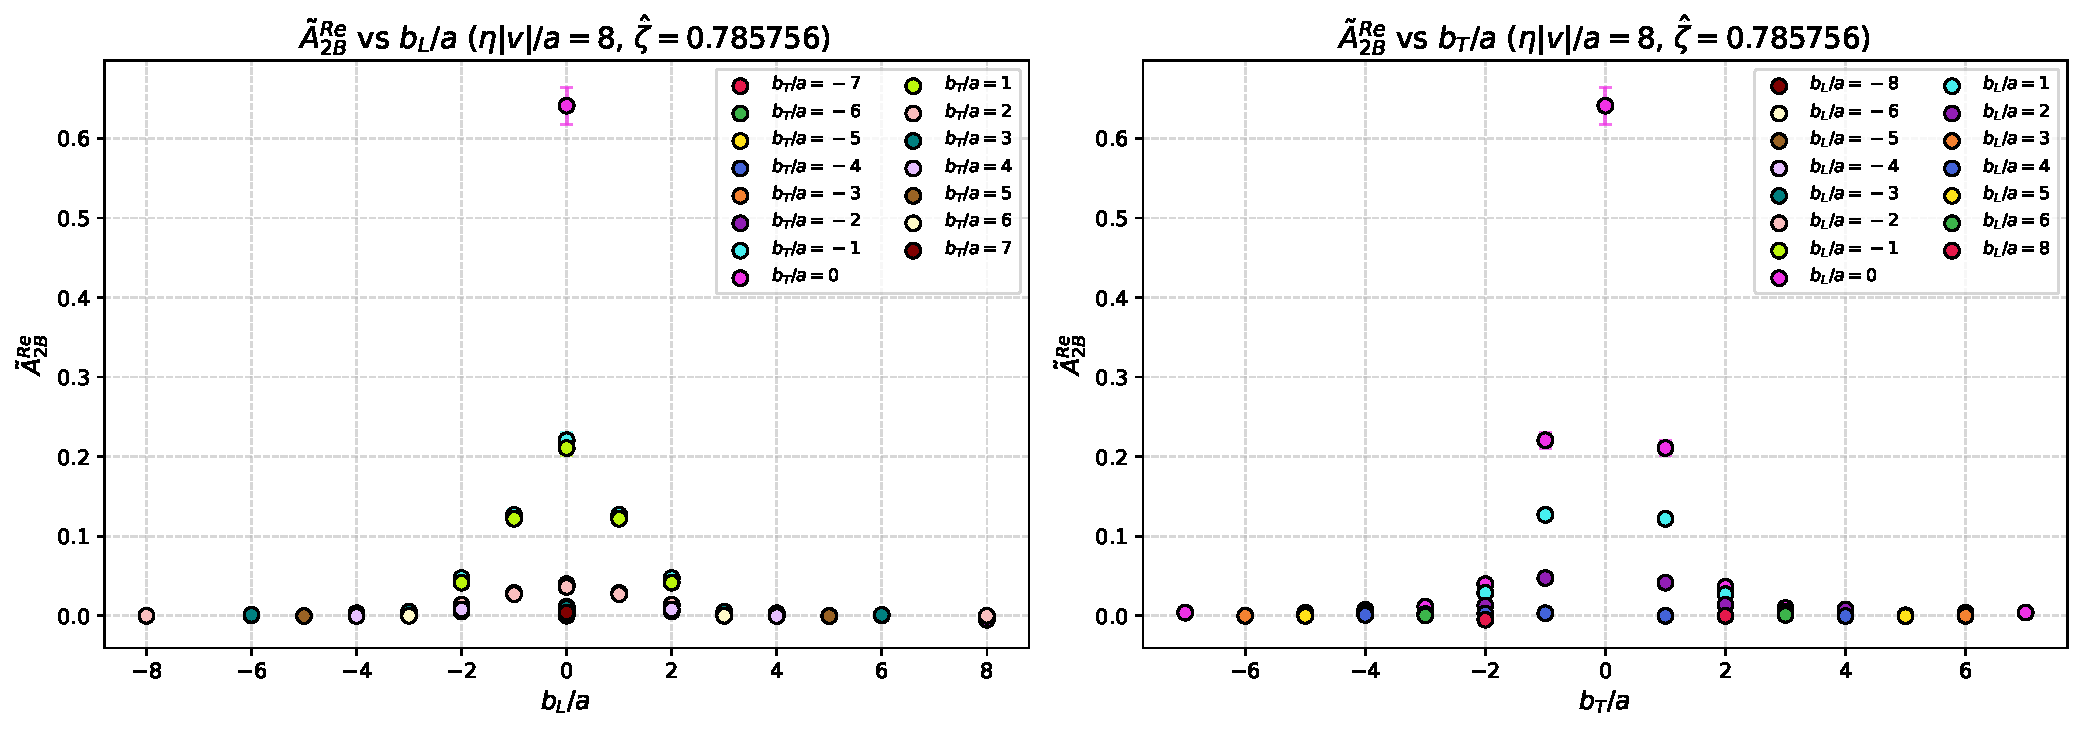
\includegraphics[width=0.98\linewidth,height=0.73\textheight,keepaspectratio]{ReA2B_eta8_PL-4_2D.pdf}\\[1mm]
{\small $\zetahat=0.785756$; $(b_L,b_T)$; $\eta|v|/a=8$ slices}
\figsrc{Thesis, Ch. 5: raw amplitude profiles; complete original panels.}
\end{frame}

\begin{frame}{$\tAmp_{2B}^{\mathrm{Re}}$ at $P_L=-4$: invariant coordinates}
\centering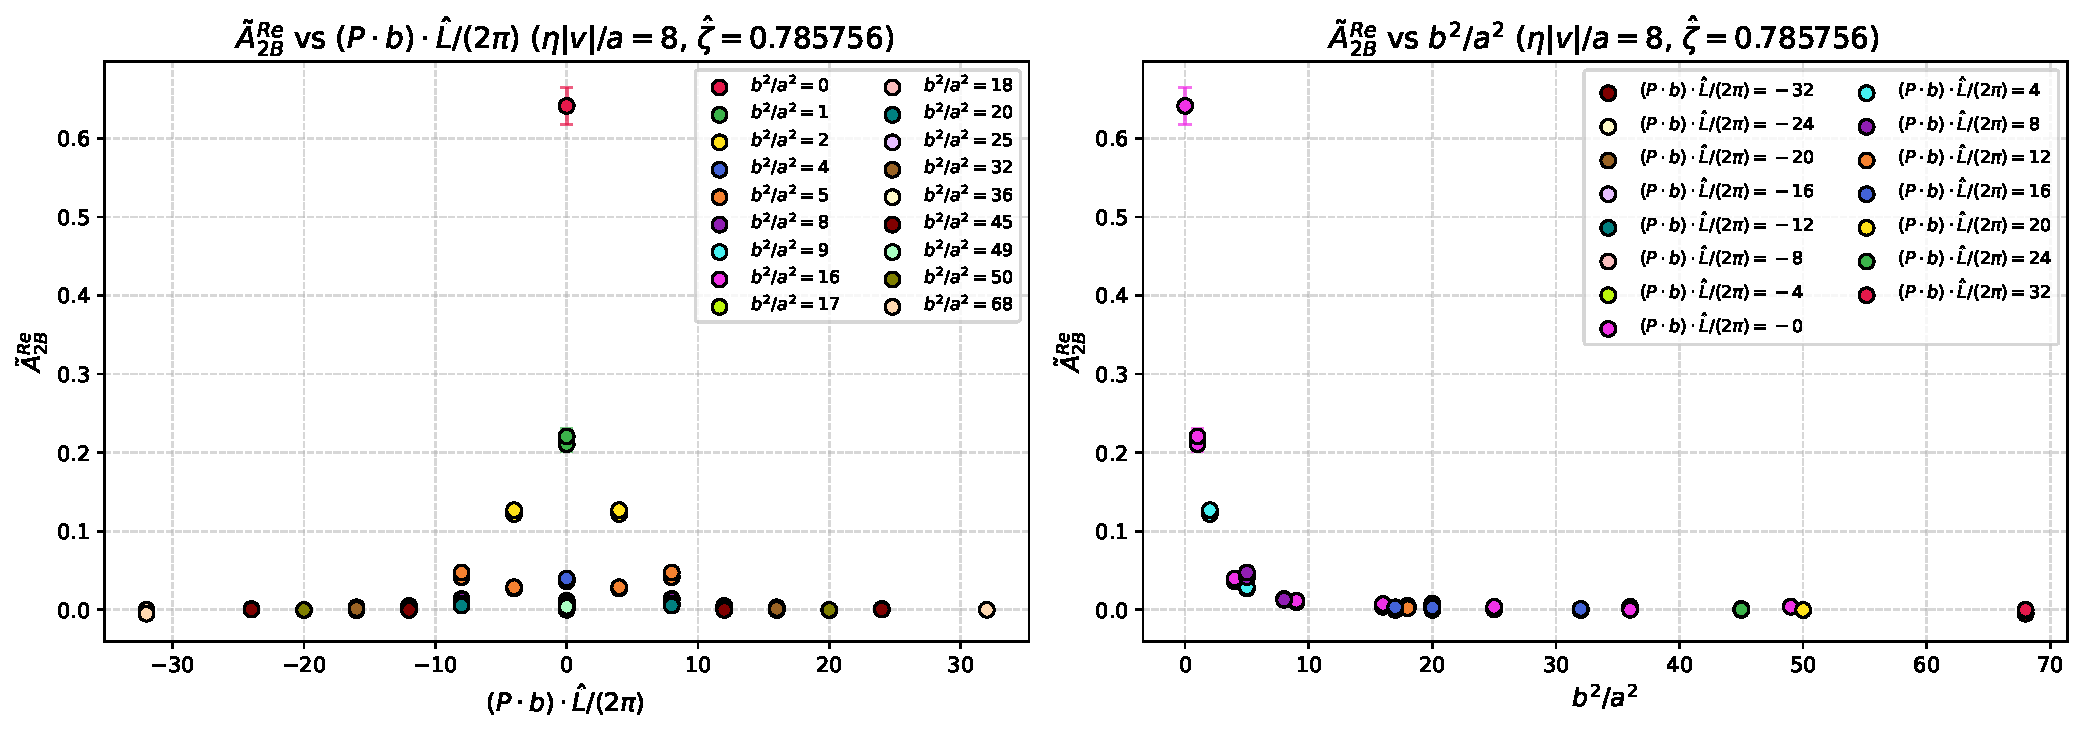
\includegraphics[width=0.98\linewidth,height=0.73\textheight,keepaspectratio]{ReA2B_Pb_bsq_eta8_PL-4_2D.pdf}\\[1mm]
{\small $\zetahat=0.785756$; $(\nu,s)$; $\eta|v|/a=8$ slices}
\figsrc{Thesis, Ch. 5: raw amplitude profiles; complete original panels.}
\end{frame}

\begin{frame}{$\tAmp_{2B}^{\mathrm{Im}}$ at $P_L=-4$: lattice coordinates}
\centering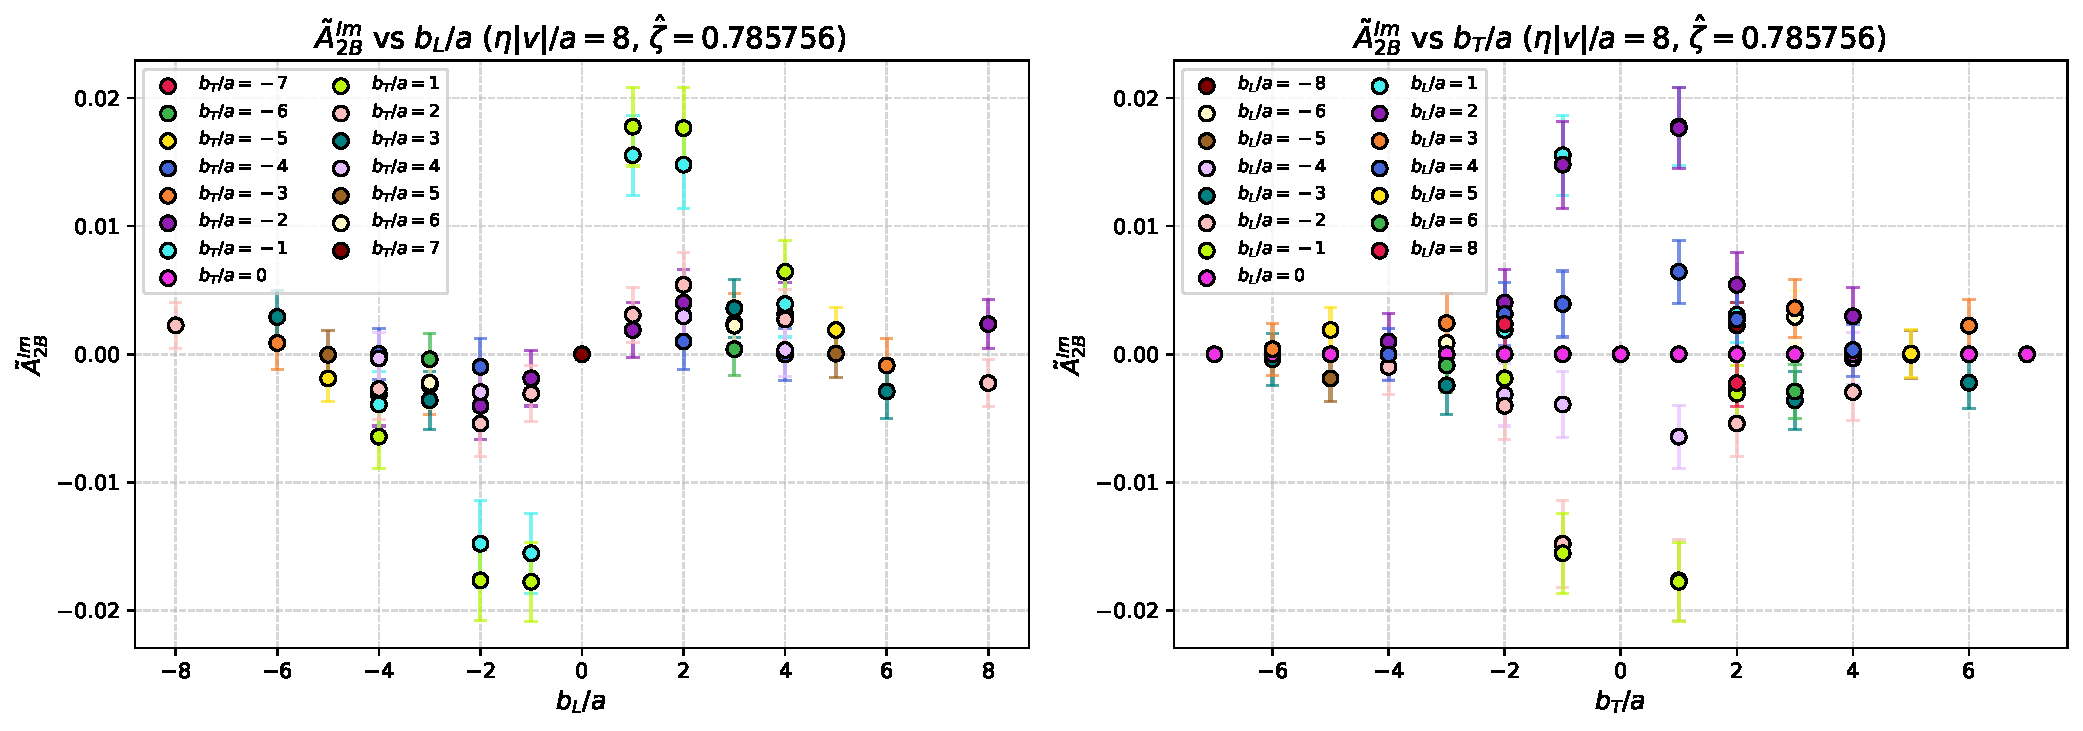
\includegraphics[width=0.98\linewidth,height=0.73\textheight,keepaspectratio]{ImA2B_eta8_PL-4_2D.pdf}\\[1mm]
{\small $\zetahat=0.785756$; $(b_L,b_T)$; $\eta|v|/a=8$ slices}
\figsrc{Thesis, Ch. 5: raw amplitude profiles; complete original panels.}
\end{frame}

\begin{frame}{$\tAmp_{2B}^{\mathrm{Im}}$ at $P_L=-4$: invariant coordinates}
\centering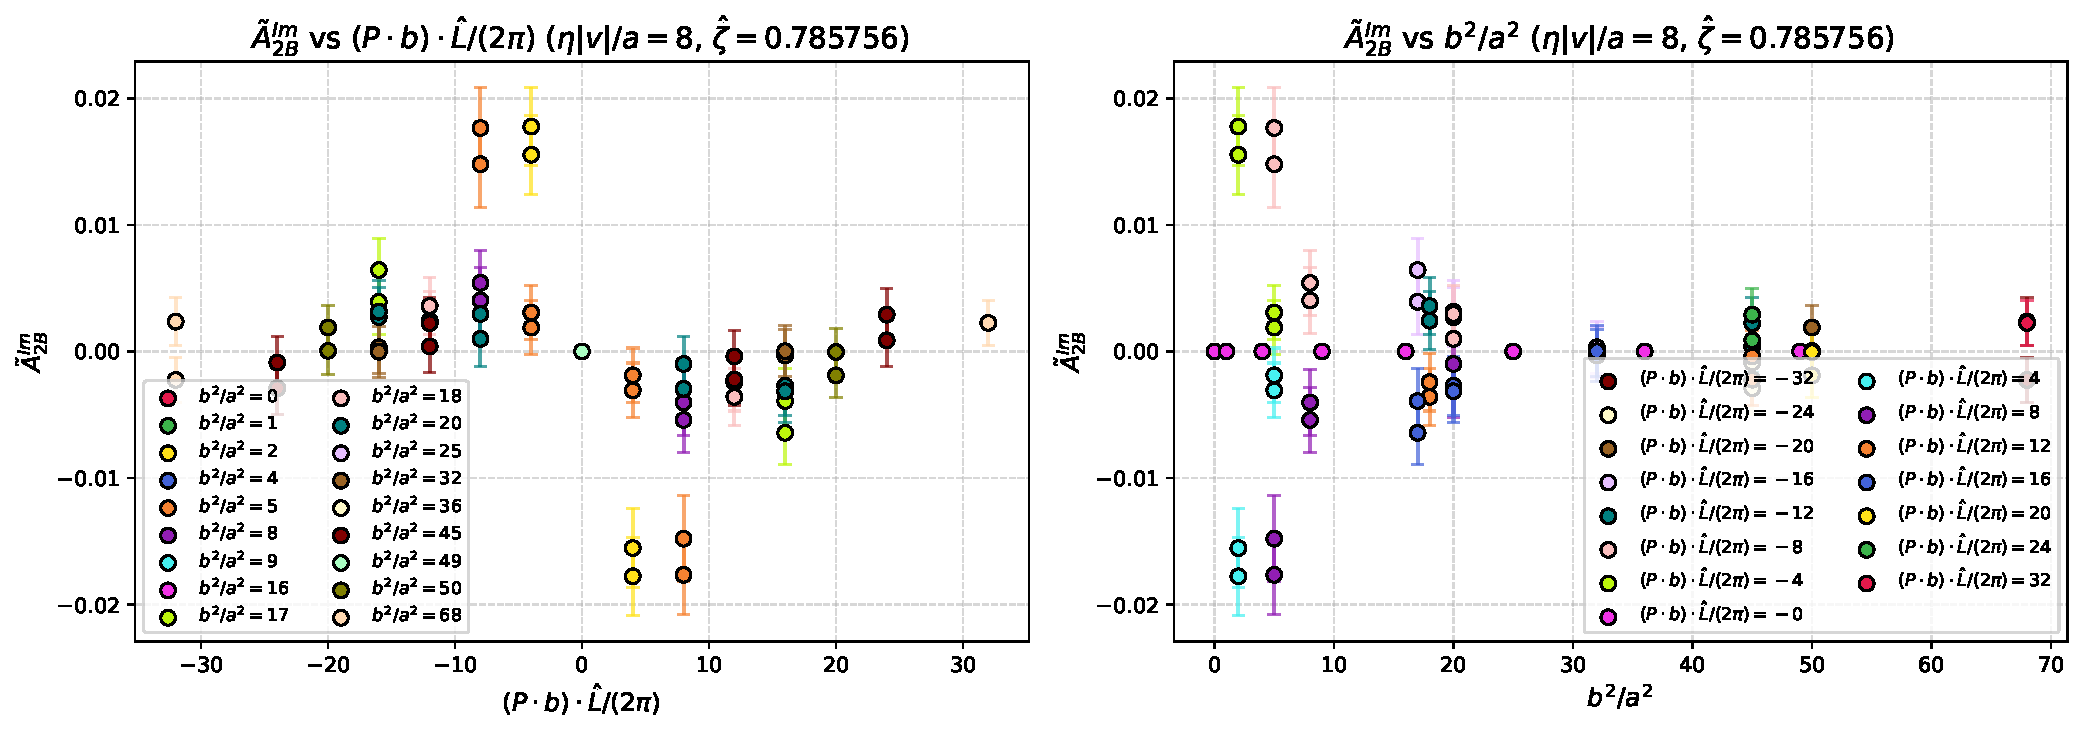
\includegraphics[width=0.98\linewidth,height=0.73\textheight,keepaspectratio]{ImA2B_Pb_bsq_eta8_PL-4_2D.pdf}\\[1mm]
{\small $\zetahat=0.785756$; $(\nu,s)$; $\eta|v|/a=8$ slices}
\figsrc{Thesis, Ch. 5: raw amplitude profiles; complete original panels.}
\end{frame}

\begin{frame}{$\tAmp_{12B}^{\mathrm{Re}}$ at $P_L=-4$: lattice coordinates}
\centering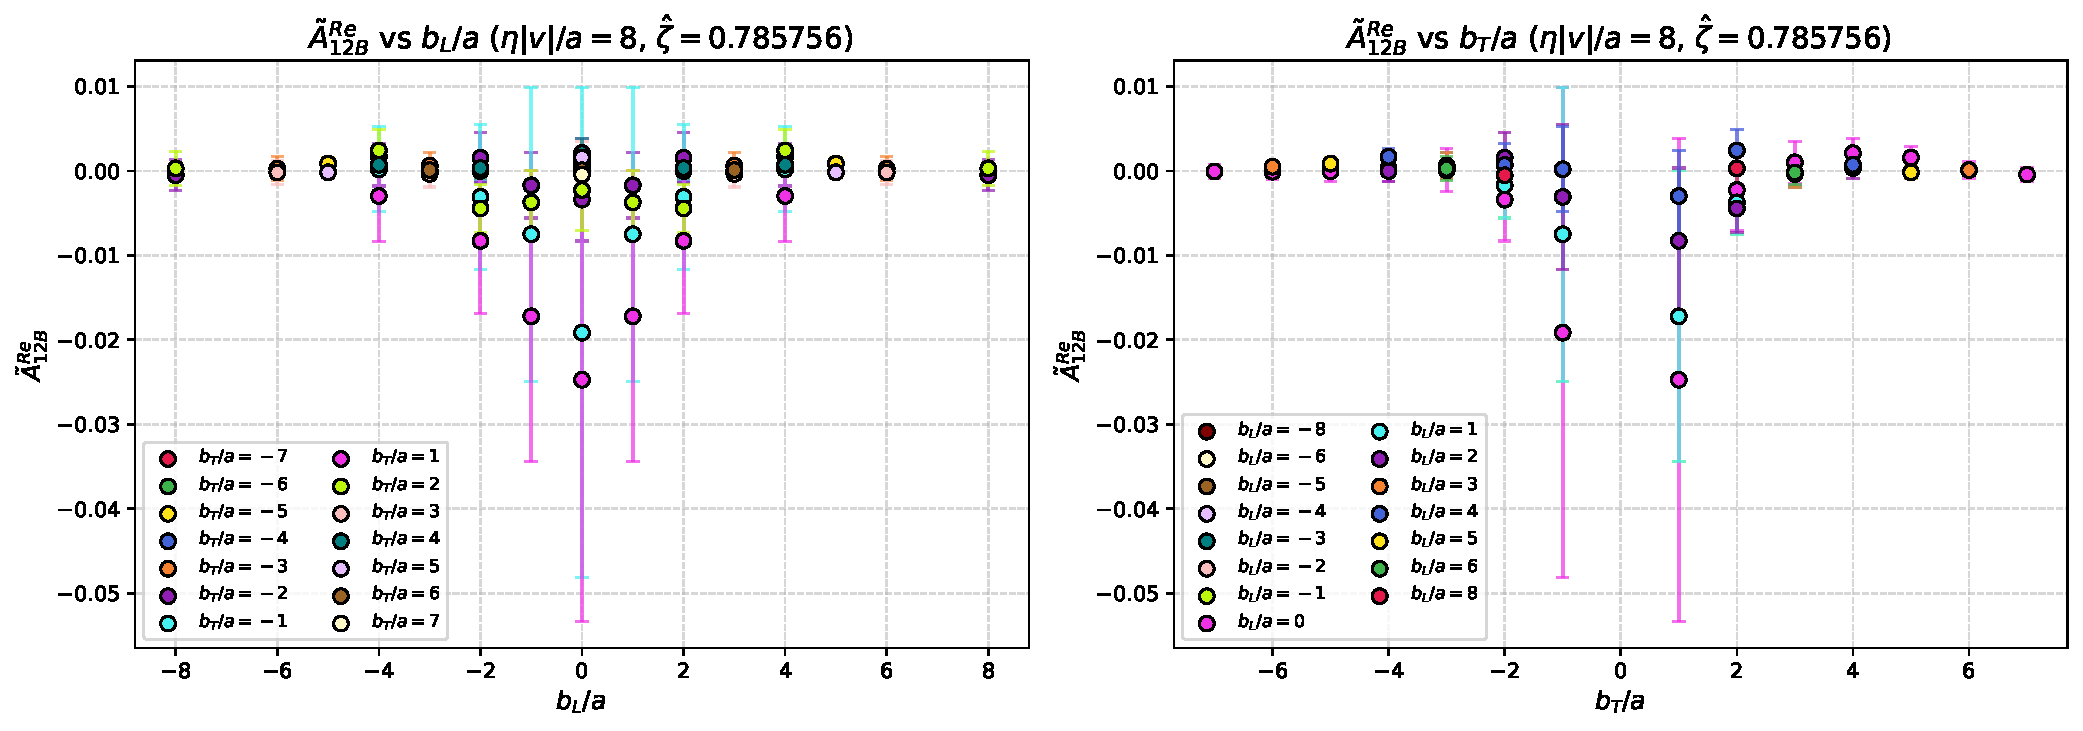
\includegraphics[width=0.98\linewidth,height=0.73\textheight,keepaspectratio]{ReA12B_eta8_PL-4_2D.pdf}\\[1mm]
{\small $\zetahat=0.785756$; $(b_L,b_T)$; $\eta|v|/a=8$ slices}
\figsrc{Thesis, Ch. 5: raw amplitude profiles; complete original panels.}
\end{frame}

\begin{frame}{$\tAmp_{12B}^{\mathrm{Re}}$ at $P_L=-4$: invariant coordinates}
\centering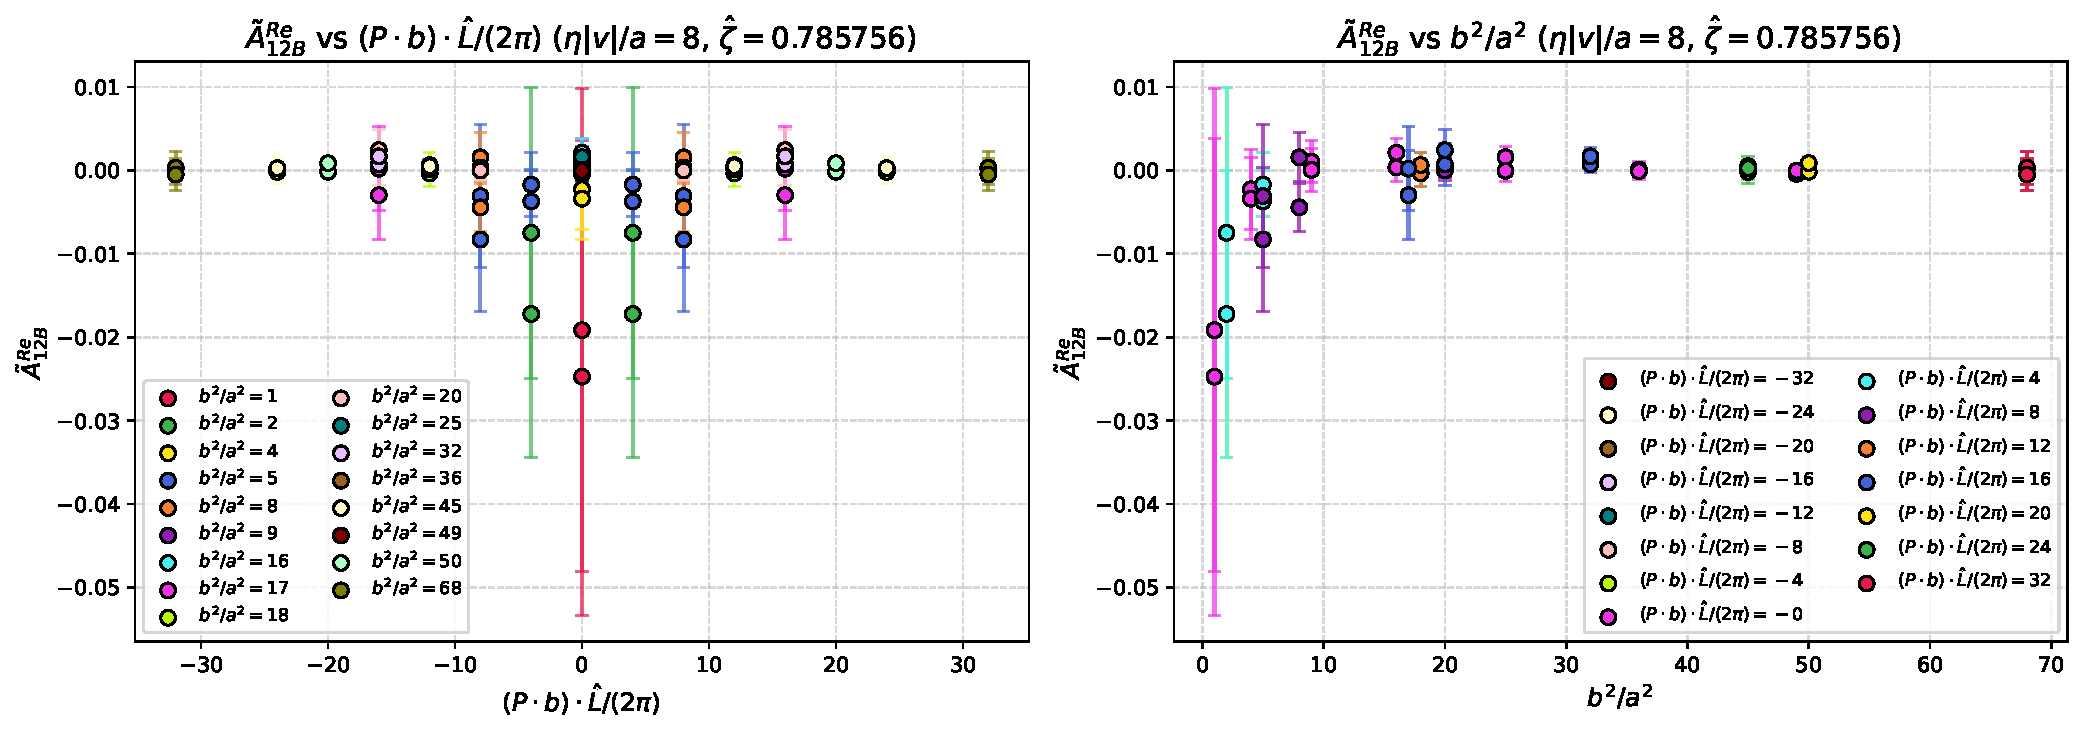
\includegraphics[width=0.98\linewidth,height=0.73\textheight,keepaspectratio]{ReA12B_Pb_bsq_eta8_PL-4_2D.pdf}\\[1mm]
{\small $\zetahat=0.785756$; $(\nu,s)$; $\eta|v|/a=8$ slices}
\figsrc{Thesis, Ch. 5: raw amplitude profiles; complete original panels.}
\end{frame}

\begin{frame}{$\tAmp_{12B}^{\mathrm{Im}}$ at $P_L=-4$: lattice coordinates}
\centering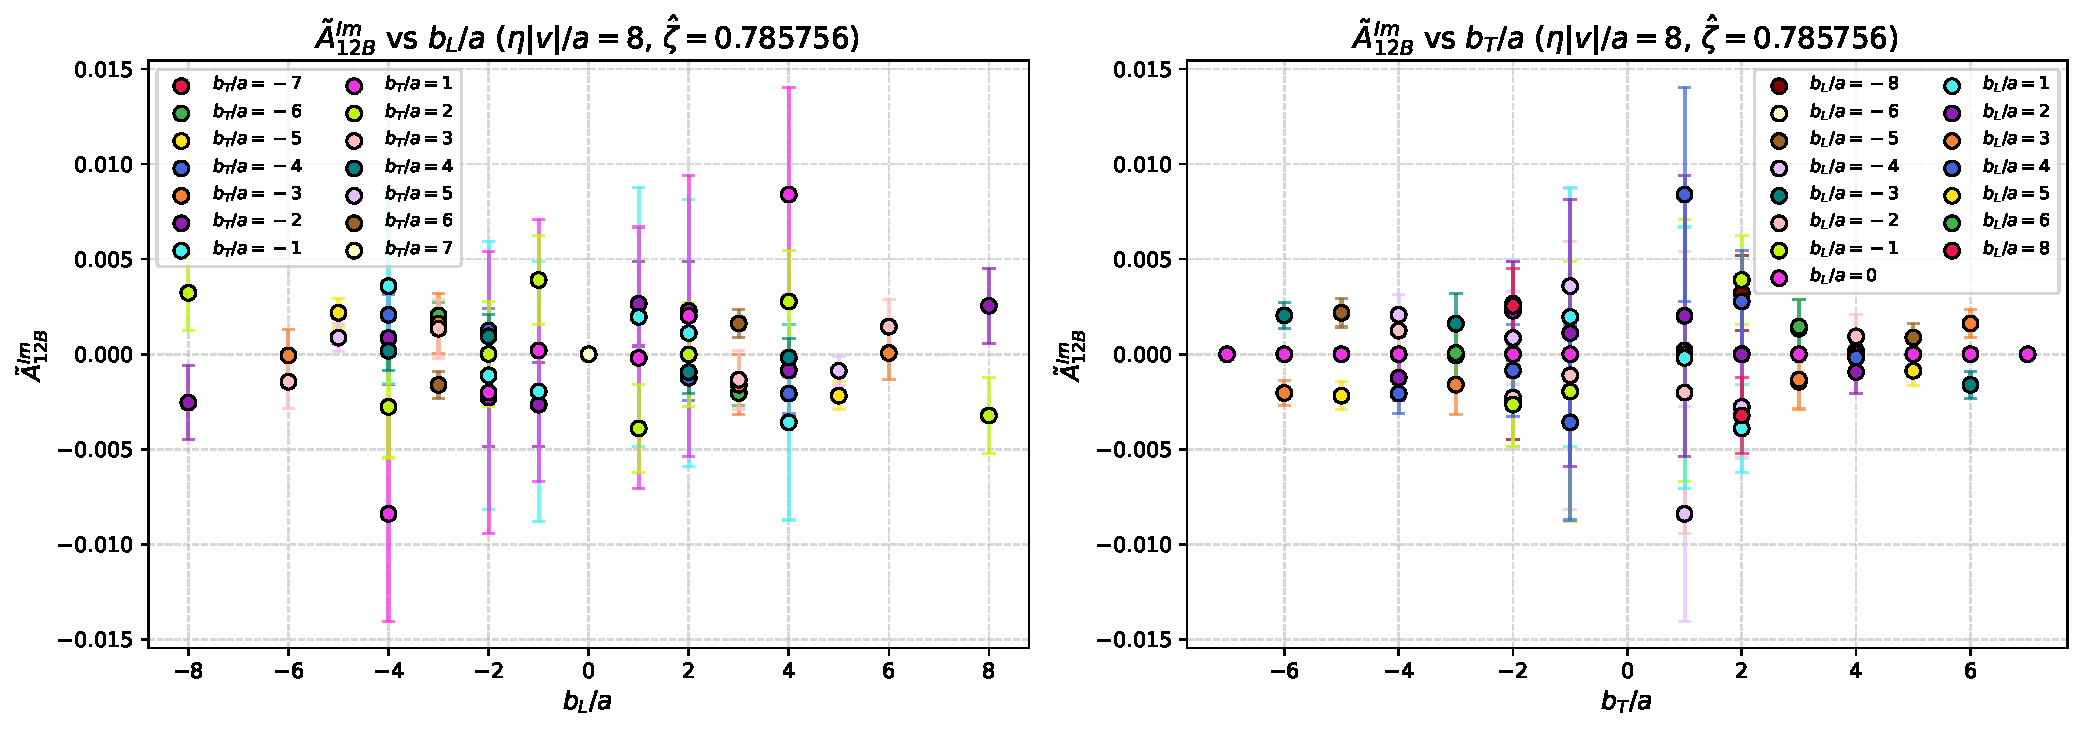
\includegraphics[width=0.98\linewidth,height=0.73\textheight,keepaspectratio]{ImA12B_eta8_PL-4_2D.pdf}\\[1mm]
{\small $\zetahat=0.785756$; $(b_L,b_T)$; $\eta|v|/a=8$ slices}
\figsrc{Thesis, Ch. 5: raw amplitude profiles; complete original panels.}
\end{frame}

\begin{frame}{$\tAmp_{12B}^{\mathrm{Im}}$ at $P_L=-4$: invariant coordinates}
\centering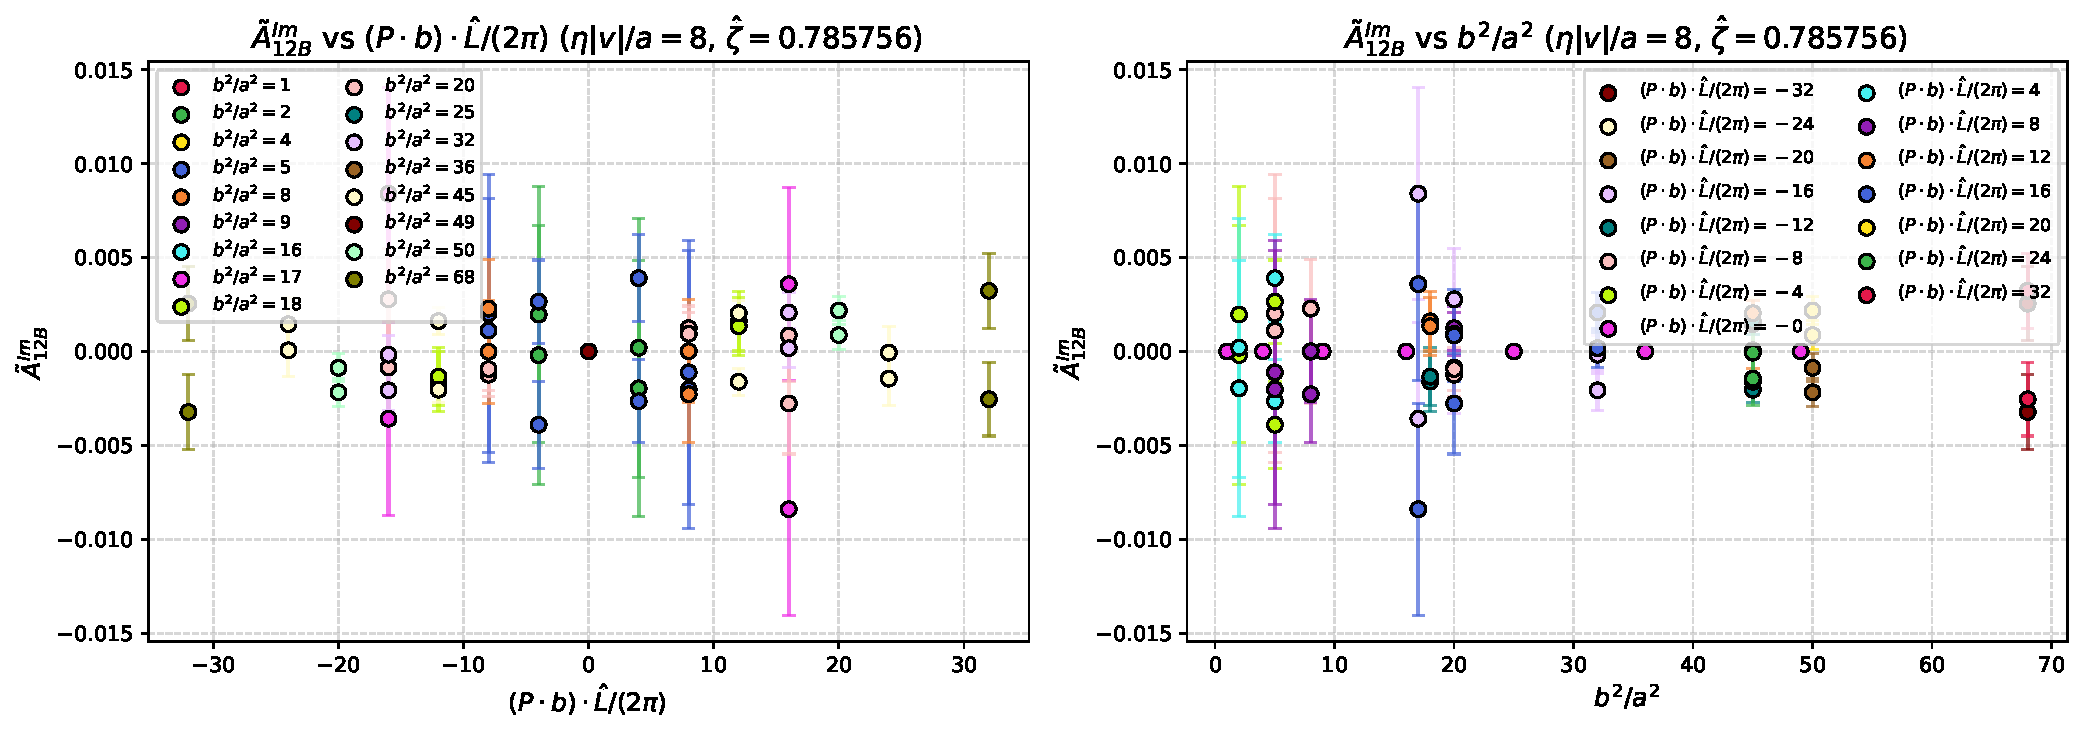
\includegraphics[width=0.98\linewidth,height=0.73\textheight,keepaspectratio]{ImA12B_Pb_bsq_eta8_PL-4_2D.pdf}\\[1mm]
{\small $\zetahat=0.785756$; $(\nu,s)$; $\eta|v|/a=8$ slices}
\figsrc{Thesis, Ch. 5: raw amplitude profiles; complete original panels.}
\end{frame}


\begin{frame}{Parity and the imaginary Sivers amplitude}
  \[
    \tAmp_{iB}^{\mathrm{Re}}(-\nu)=\tAmp_{iB}^{\mathrm{Re}}(\nu),\qquad
    \tAmp_{iB}^{\mathrm{Im}}(-\nu)=-\tAmp_{iB}^{\mathrm{Im}}(\nu).
  \]
  \begin{itemize}
    \item The profiles display the parity imposed by the amplitude projection; this is a consistency check of the extraction.
    \item The thesis finds no statistically resolved $\tAmp_{12B}^{\mathrm{Im}}$ signal and omits it from the subsequent fit. Compatibility with zero does not establish that it vanishes exactly.
    \item With this analysis choice, write $E=E_2$, $O=O_2$, $S=E_{12}$:
  \end{itemize}
  \[ \tilde f_1^{(0)}=2(E-O),\qquad
      \tilde f_{1T}^{\perp(1)}=-2S,\qquad
      \langle k_y\rangle_{TU}=-m_N\frac{S}{E-O}. \]
  \figsrc{Thesis, Ch. 5: numerical profiles and treatment of $\tAmp_{12B}^{\mathrm{Im}}$.}
\end{frame}
